%--------------------------------------
%ELECTROTECHNIQUE - SCHEMA DE LIAISON A LA TERRE
%--------------------------------------

%utiliser les environnement \begin{comment} \end{comment} pour mettre en commentaire le préambule une fois la programmation appelée dans le document maître (!ne pas oublier de mettre en commentaire \end{document}!)

\begin{comment}

\documentclass[a4paper, 11pt, twoside, fleqn]{memoir}

\usepackage{AOCDTF}

\marqueurchapitre
\decoupagechapitre{1} %juste pour éviter les erreurs lors de la compilation des sous-programmations (passera en commentaire)

%--------------------------------------
%corps du document
%--------------------------------------

\begin{document} %corps du document
	\openleft %début de chapitre à gauche

\end{comment}

\chapter{Schéma Impédant-Terre\label{chap:schema_it}}
\ChapFrame

\section{Caractéristiques générales}

\begin{definition}{Schéma IT}{}
Schéma de liaison à la terre dans lequel le prise de terre du neutre du transformateur et la prise de terre des masses métalliques sont raccordées à la terre selon quatre variantes différentes :
\begin{description}
\item [Neutre :] isolé du point neutre du transformateur HT/BT (complètement isolé ou via une \emph{impédance de limitation})\,;
\item [Masses :] reliées à la terre (interconnectées ou individuellement).
\end{description}
\end{definition}

\begin{table}[H]
\caption{Détail sur les variantes de branchement en schéma IT}
\begin{tabularx}{\linewidth}{XXXX}
\toprule
\multicolumn{2}{c}{\thead{Neutre transformateur HT/BT}} & \multicolumn{2}{c}{\thead{Masses conductrices}} \\
\cmidrule(lr){1-2} 	\cmidrule(lr){3-4}
\thead{Isolé ($Z_{res}$)}	& \thead{Impédant ($Z_{N}$)}	& \thead{Interconnectées}	& \thead{Individuelles} \\
\midrule
Neutre du transformateur pas raccordé du tout. Terme \og isolé \fg{} à nuancer car l'installation électrique en aval du transformateur HT/BT ne sera jamais complètement isolée par rapport à la terre. Il subsistera toujours un courant de défaut $I_d$ plus ou moins minime due à une impédance de fuite $Z_{res}$ présente dans tous les réseaux électriques (voir \superref{sec:isolation_installation_schema_it}).
& 
Neutre du transformateur raccordé à la prise de terre par une \emph{impédance de limitation} dont la valeur dépend de la fréquence de la tension :
\begin{compactitemize}
\item$F=\SI{50}{\hertz}$ : \SI{1500}{\ohm}\,;
\item$F=\SI{2,5}{\hertz}$ : \SI{2,5}{\ohm}.
\end{compactitemize}
Cette impédance fixe donc une différence de potentiel définie entre le neutre et la terre, elle est installée lorsque le réseau électrique est court et que l'impédance de fuite $Z_{res}$ est élevée.
&
Masses \emph{interconnectées} au moyen d'un conducteur PE et raccordées à la terre au niveau du transformateur HT/BT. Raccordement similaire au schéma TN, à la différence que le neutre du transformateur n'est pas raccordé au conducteur PE et à la terre.
&
Masses mise à la terre \emph{individuellement} ou par groupe à des prises de terre propres. Type de raccordement similaire au schéma TT avec installation de DDR en tête de chaque circuit. \\
\bottomrule
\end{tabularx}
\end{table}

Il s'agit d'un SLT un peu plus atypique ayant pour but d'assurer une \emph{continuité de service} à l'installation électrique malgré un \emph{premier défaut d'isolement} tout en assurant la protection des personnes contre les contacts indirects. Selon les quatre variantes de raccordement, le premier défaut entrainera un fonctionnement identique des protections mais à l'apparition d'un deuxième défaut entrainera un fonctionnement des protection différent.\\

Dans la pratique, le schéma IT présente les caractéristiques suivantes :
\begin{itemize}
\item continuité de service assurée après un premier défaut d'isolement\,;
\item contrôle permanent de l'isolement de l'installation par rapport à la terre avec signalisation de toute dépassement du seuil d'isolement défini à l'aide d'un Contrôleur Permanent d'Isolement (CPI)\,;
\item protection du neutre assurée\,;
\item raccordement possible d'un limiteur de tension (éclateur) entre la terre et le point neutre du transformateur HT/BT\,;
\item présence continue d'une équipe pour assurer rapidement la recherche du premier défaut d'isolement aussitôt signalé, facilitée avec du matériel de localisation automatique\,;
\item coupure automatique de l'installation dès l'apparition d'un second défaut d'isolement sur un conducteur actif différent de celui ou le premier défaut d'isolement est apparu.
\end{itemize}

Le courant de défaut du premier défaut d'isolement va dépendre de l'impédance de limitation du neutre et de l'état d'isolement de l'installation électrique. Pour toutefois protéger les personnes, il doit être suffisamment bas pour satisfaire la règle $I_{d} \times R_{A} \pm \SI{50}{\volt}$, de sorte à ce que la tension de défaut $U_d$ ne présente aucun danger.

\section{Isolation de l'installation électrique en schéma IT\label{sec:isolation_installation_schema_it}}

Dans le cas d'un schéma IT ou le neutre est isolé, l'isolement de l'installation de l'installation électrique n'est pas infini par rapport à la terre car les isolants ne présentent jamais une résistance infinie. Une résistance de fuite du de l'installation électrique apparaitra toujours et dépendra de plusieurs facteurs :
\begin{itemize}
\item nature des isolants (PVC, air\ldots)\,;
\item âge de l'installation
\item degré d'humidité\,;
\item longueur de l'installation.
\end{itemize}
Pour une installation neuve, on considère que la résistance de fuite est estimée à \SI{3,3}{\mega\ohm} pour \SI{1}{\kilo\meter} de réseau électrique.

\begin{formule}{Résistance de fuite du réseaux $R_{res}$ d'une installation neuve}{}
\begin{align*}
	R_{res} &= \frac{3,3}{n}
\end{align*} 
\begin{textvariables}
R_{res}						& résistance					& méga-ohm			& \mega\ohm							& 	Résistance de fuite du réseaux électrique \\
n								& 									& 							& /										& 	Nombre de \si{\kilo\meter} de réseaux électrique \\
\end{textvariables}
\end{formule}

%--------------------------------------
%ELECTROTECHNIQUE - SCHEMA DE LIAISON A LA TERRE
%--------------------------------------

%utiliser les environnement \begin{comment} \end{comment} pour mettre en commentaire le préambule une fois la programmation appelée dans le document maître (!ne pas oublier de mettre en commentaire \end{document}!)

\begin{comment}

\documentclass[a4paper, 11pt, twoside, fleqn]{memoir}

\usepackage{AOCDTF}

\marqueurchapitre
\decoupagechapitre{1} %juste pour éviter les erreurs lors de la compilation des sous-programmations (passera en commentaire)

%lien d'édition des figures Tikz sur le site mathcha.io (rajouter le lien d'une modification effectuée sur la figure tikz avec le nom du modificateur car il n'y a qu'un lien par compte)

%lien mathcha Bruno Douchy : https://www.mathcha.io/editor/Kxxn3cWBUm3T7ynYmWi4KY0P9H9d6v9qFLQyMEE

%--------------------------------------
%corps du document
%--------------------------------------

\begin{document} %corps du document
	\openleft %début de chapitre à gauche

\end{comment}


% Pattern Info
\begin{figure}[H]
\caption{Résistance de fuite $R_{res}$ d'un réseau électrique de plusieurs \si{\kilo\meter}}

% Pattern Info
 
\tikzset{
pattern size/.store in=\mcSize, 
pattern size = 5pt,
pattern thickness/.store in=\mcThickness, 
pattern thickness = 0.3pt,
pattern radius/.store in=\mcRadius, 
pattern radius = 1pt}
\makeatletter
\pgfutil@ifundefined{pgf@pattern@name@_sgw0g8yxt}{
\pgfdeclarepatternformonly[\mcThickness,\mcSize]{_sgw0g8yxt}
{\pgfqpoint{0pt}{0pt}}
{\pgfpoint{\mcSize+\mcThickness}{\mcSize+\mcThickness}}
{\pgfpoint{\mcSize}{\mcSize}}
{
\pgfsetcolor{\tikz@pattern@color}
\pgfsetlinewidth{\mcThickness}
\pgfpathmoveto{\pgfqpoint{0pt}{0pt}}
\pgfpathlineto{\pgfpoint{\mcSize+\mcThickness}{\mcSize+\mcThickness}}
\pgfusepath{stroke}
}}
\makeatother
\tikzset{every picture/.style={line width=0.75pt}} %set default line width to 0.75pt        

\begin{tikzpicture}[x=0.75pt,y=0.75pt,yscale=-1,xscale=1]
%uncomment if require: \path (0,327); %set diagram left start at 0, and has height of 327

%Straight Lines [id:da08009100326878149] 
\draw    (105,35) -- (210,35) ;
%Shape: Circle [id:dp3640107906362746] 
\draw   (2.5,35) .. controls (2.5,18.43) and (15.93,5) .. (32.5,5) .. controls (49.07,5) and (62.5,18.43) .. (62.5,35) .. controls (62.5,51.57) and (49.07,65) .. (32.5,65) .. controls (15.93,65) and (2.5,51.57) .. (2.5,35) -- cycle ;
%Straight Lines [id:da571377768464931] 
\draw    (30,232.5) -- (545,232.5) ;
%Straight Lines [id:da08045007432417306] 
\draw    (210,247.5) -- (210,262.5) ;
%Straight Lines [id:da4313577623259258] 
\draw    (200,262.5) -- (220,262.5) ;
%Straight Lines [id:da5912684771420953] 
\draw    (202.5,267.5) -- (217.5,267.5) ;
%Straight Lines [id:da13165123057200734] 
\draw    (205,272.5) -- (215,272.5) ;

%Straight Lines [id:da320941654963934] 
\draw    (210,217.5) -- (210,222.5) ;
%Shape: Rectangle [id:dp24059175551770873] 
\draw   (215,187.5) -- (215,217.5) -- (205,217.5) -- (205,187.5) -- cycle ;
%Straight Lines [id:da9352215304977288] 
\draw    (210,182.5) -- (210,187.5) ;

%Shape: Circle [id:dp5173960999636192] 
\draw   (45,35) .. controls (45,18.43) and (58.43,5) .. (75,5) .. controls (91.57,5) and (105,18.43) .. (105,35) .. controls (105,51.57) and (91.57,65) .. (75,65) .. controls (58.43,65) and (45,51.57) .. (45,35) -- cycle ;
%Straight Lines [id:da826385807465586] 
\draw    (140,45) -- (150,25) ;
\draw [shift={(150,25)}, rotate = 296.57] [color={rgb, 255:red, 0; green, 0; blue, 0 }  ][fill={rgb, 255:red, 0; green, 0; blue, 0 }  ][line width=0.75]      (0, 0) circle [x radius= 2.01, y radius= 2.01]   ;
%Straight Lines [id:da9637899679537502] 
\draw    (120,45) -- (130,25) ;
%Straight Lines [id:da6640472127950414] 
\draw    (115,45) -- (125,25) ;
%Straight Lines [id:da46557993038086076] 
\draw    (110,45) -- (120,25) ;

%Straight Lines [id:da33735776097392156] 
\draw    (210,222.5) -- (210,247.5) ;
%Straight Lines [id:da5122217943063542] 
\draw    (210,35) -- (210,182.5) ;
%Shape: Circle [id:dp05291492243843332] 
\draw  [fill={rgb, 255:red, 0; green, 0; blue, 0 }  ,fill opacity=1 ] (207.5,35) .. controls (207.5,33.62) and (208.62,32.5) .. (210,32.5) .. controls (211.38,32.5) and (212.5,33.62) .. (212.5,35) .. controls (212.5,36.38) and (211.38,37.5) .. (210,37.5) .. controls (208.62,37.5) and (207.5,36.38) .. (207.5,35) -- cycle ;
%Straight Lines [id:da6377337353392218] 
\draw    (212.5,35) -- (317.5,35) ;
%Straight Lines [id:da25115314727149973] 
\draw    (317.5,247.5) -- (317.5,262.5) ;
%Straight Lines [id:da901440360563758] 
\draw    (307.5,262.5) -- (327.5,262.5) ;
%Straight Lines [id:da7842646096579663] 
\draw    (310,267.5) -- (325,267.5) ;
%Straight Lines [id:da18808830899848483] 
\draw    (312.5,272.5) -- (322.5,272.5) ;

%Straight Lines [id:da49919296084643217] 
\draw    (317.5,217.5) -- (317.5,222.5) ;
%Shape: Rectangle [id:dp5156050966431545] 
\draw   (322.5,187.5) -- (322.5,217.5) -- (312.5,217.5) -- (312.5,187.5) -- cycle ;
%Straight Lines [id:da9531373030412352] 
\draw    (317.5,182.5) -- (317.5,187.5) ;

%Straight Lines [id:da8099985845539385] 
\draw    (247.5,45) -- (257.5,25) ;
\draw [shift={(257.5,25)}, rotate = 296.57] [color={rgb, 255:red, 0; green, 0; blue, 0 }  ][fill={rgb, 255:red, 0; green, 0; blue, 0 }  ][line width=0.75]      (0, 0) circle [x radius= 2.01, y radius= 2.01]   ;
%Straight Lines [id:da8087453766565224] 
\draw    (227.5,45) -- (237.5,25) ;
%Straight Lines [id:da3541011282357912] 
\draw    (222.5,45) -- (232.5,25) ;
%Straight Lines [id:da4838872480993197] 
\draw    (217.5,45) -- (227.5,25) ;

%Straight Lines [id:da6527379034333531] 
\draw    (317.5,222.5) -- (317.5,247.5) ;
%Straight Lines [id:da5530613085402983] 
\draw    (317.5,35) -- (317.5,182.5) ;
%Shape: Circle [id:dp25176527117973546] 
\draw  [fill={rgb, 255:red, 0; green, 0; blue, 0 }  ,fill opacity=1 ] (315,35) .. controls (315,33.62) and (316.12,32.5) .. (317.5,32.5) .. controls (318.88,32.5) and (320,33.62) .. (320,35) .. controls (320,36.38) and (318.88,37.5) .. (317.5,37.5) .. controls (316.12,37.5) and (315,36.38) .. (315,35) -- cycle ;
%Straight Lines [id:da18023630680839797] 
\draw    (320,35) -- (425,35) ;
%Straight Lines [id:da6476101136895756] 
\draw    (425,247.5) -- (425,262.5) ;
%Straight Lines [id:da4732182664219796] 
\draw    (415,262.5) -- (435,262.5) ;
%Straight Lines [id:da9789341071401707] 
\draw    (417.5,267.5) -- (432.5,267.5) ;
%Straight Lines [id:da9061441462289892] 
\draw    (420,272.5) -- (430,272.5) ;

%Straight Lines [id:da5168046359577328] 
\draw    (425,217.5) -- (425,222.5) ;
%Shape: Rectangle [id:dp6616267367458876] 
\draw   (430,187.5) -- (430,217.5) -- (420,217.5) -- (420,187.5) -- cycle ;
%Straight Lines [id:da5013364563135433] 
\draw    (425,182.5) -- (425,187.5) ;

%Straight Lines [id:da8467083023662558] 
\draw    (355,45) -- (365,25) ;
\draw [shift={(365,25)}, rotate = 296.57] [color={rgb, 255:red, 0; green, 0; blue, 0 }  ][fill={rgb, 255:red, 0; green, 0; blue, 0 }  ][line width=0.75]      (0, 0) circle [x radius= 2.01, y radius= 2.01]   ;
%Straight Lines [id:da8678289301466517] 
\draw    (335,45) -- (345,25) ;
%Straight Lines [id:da902125655347565] 
\draw    (330,45) -- (340,25) ;
%Straight Lines [id:da33092289865462876] 
\draw    (325,45) -- (335,25) ;

%Straight Lines [id:da6870106618089796] 
\draw    (425,222.5) -- (425,247.5) ;
%Straight Lines [id:da01716755816154636] 
\draw    (425,35) -- (425,182.5) ;
%Shape: Circle [id:dp22065699926749582] 
\draw  [fill={rgb, 255:red, 0; green, 0; blue, 0 }  ,fill opacity=1 ] (422.5,35) .. controls (422.5,33.62) and (423.62,32.5) .. (425,32.5) .. controls (426.38,32.5) and (427.5,33.62) .. (427.5,35) .. controls (427.5,36.38) and (426.38,37.5) .. (425,37.5) .. controls (423.62,37.5) and (422.5,36.38) .. (422.5,35) -- cycle ;
%Straight Lines [id:da8428146399476175] 
\draw    (427.5,35) -- (532.5,35) ;
%Straight Lines [id:da6165941111135154] 
\draw    (532.5,247.5) -- (532.5,262.5) ;
%Straight Lines [id:da22141601388795418] 
\draw    (522.5,262.5) -- (542.5,262.5) ;
%Straight Lines [id:da8768087653277724] 
\draw    (525,267.5) -- (540,267.5) ;
%Straight Lines [id:da8238869233080838] 
\draw    (527.5,272.5) -- (537.5,272.5) ;

%Straight Lines [id:da4119258117043978] 
\draw    (532.5,217.5) -- (532.5,222.5) ;
%Shape: Rectangle [id:dp20576670411827713] 
\draw   (537.5,187.5) -- (537.5,217.5) -- (527.5,217.5) -- (527.5,187.5) -- cycle ;
%Straight Lines [id:da2173028442784587] 
\draw    (532.5,182.5) -- (532.5,187.5) ;

%Straight Lines [id:da9355672330564798] 
\draw    (462.5,45) -- (472.5,25) ;
\draw [shift={(472.5,25)}, rotate = 296.57] [color={rgb, 255:red, 0; green, 0; blue, 0 }  ][fill={rgb, 255:red, 0; green, 0; blue, 0 }  ][line width=0.75]      (0, 0) circle [x radius= 2.01, y radius= 2.01]   ;
%Straight Lines [id:da16076902370326562] 
\draw    (442.5,45) -- (452.5,25) ;
%Straight Lines [id:da9307381027117236] 
\draw    (437.5,45) -- (447.5,25) ;
%Straight Lines [id:da4509037983599339] 
\draw    (432.5,45) -- (442.5,25) ;

%Straight Lines [id:da3857851833734479] 
\draw    (532.5,222.5) -- (532.5,247.5) ;
%Straight Lines [id:da6375117758137738] 
\draw    (532.5,35) -- (532.5,182.5) ;
%Shape: Circle [id:dp4200718497991244] 
\draw  [fill={rgb, 255:red, 0; green, 0; blue, 0 }  ,fill opacity=1 ] (530,35) .. controls (530,33.62) and (531.12,32.5) .. (532.5,32.5) .. controls (533.88,32.5) and (535,33.62) .. (535,35) .. controls (535,36.38) and (533.88,37.5) .. (532.5,37.5) .. controls (531.12,37.5) and (530,36.38) .. (530,35) -- cycle ;
%Straight Lines [id:da7951184635426344] 
\draw    (107,70) -- (208,70) ;
\draw [shift={(210,70)}, rotate = 180] [color={rgb, 255:red, 0; green, 0; blue, 0 }  ][line width=0.75]    (10.93,-3.29) .. controls (6.95,-1.4) and (3.31,-0.3) .. (0,0) .. controls (3.31,0.3) and (6.95,1.4) .. (10.93,3.29)   ;
\draw [shift={(105,70)}, rotate = 0] [color={rgb, 255:red, 0; green, 0; blue, 0 }  ][line width=0.75]    (10.93,-3.29) .. controls (6.95,-1.4) and (3.31,-0.3) .. (0,0) .. controls (3.31,0.3) and (6.95,1.4) .. (10.93,3.29)   ;
%Straight Lines [id:da8649629320055597] 
\draw  [dash pattern={on 4.5pt off 4.5pt}]  (105,70) -- (105,35) ;
%Straight Lines [id:da8409577043639814] 
\draw    (212,70) -- (315.5,70) ;
\draw [shift={(317.5,70)}, rotate = 180] [color={rgb, 255:red, 0; green, 0; blue, 0 }  ][line width=0.75]    (10.93,-3.29) .. controls (6.95,-1.4) and (3.31,-0.3) .. (0,0) .. controls (3.31,0.3) and (6.95,1.4) .. (10.93,3.29)   ;
\draw [shift={(210,70)}, rotate = 0] [color={rgb, 255:red, 0; green, 0; blue, 0 }  ][line width=0.75]    (10.93,-3.29) .. controls (6.95,-1.4) and (3.31,-0.3) .. (0,0) .. controls (3.31,0.3) and (6.95,1.4) .. (10.93,3.29)   ;
%Straight Lines [id:da9560686473702245] 
\draw    (319.5,70) -- (423,70) ;
\draw [shift={(425,70)}, rotate = 180] [color={rgb, 255:red, 0; green, 0; blue, 0 }  ][line width=0.75]    (10.93,-3.29) .. controls (6.95,-1.4) and (3.31,-0.3) .. (0,0) .. controls (3.31,0.3) and (6.95,1.4) .. (10.93,3.29)   ;
\draw [shift={(317.5,70)}, rotate = 0] [color={rgb, 255:red, 0; green, 0; blue, 0 }  ][line width=0.75]    (10.93,-3.29) .. controls (6.95,-1.4) and (3.31,-0.3) .. (0,0) .. controls (3.31,0.3) and (6.95,1.4) .. (10.93,3.29)   ;
%Straight Lines [id:da009892362184173997] 
\draw    (427,70) -- (530.5,70) ;
\draw [shift={(532.5,70)}, rotate = 180] [color={rgb, 255:red, 0; green, 0; blue, 0 }  ][line width=0.75]    (10.93,-3.29) .. controls (6.95,-1.4) and (3.31,-0.3) .. (0,0) .. controls (3.31,0.3) and (6.95,1.4) .. (10.93,3.29)   ;
\draw [shift={(425,70)}, rotate = 0] [color={rgb, 255:red, 0; green, 0; blue, 0 }  ][line width=0.75]    (10.93,-3.29) .. controls (6.95,-1.4) and (3.31,-0.3) .. (0,0) .. controls (3.31,0.3) and (6.95,1.4) .. (10.93,3.29)   ;
%Shape: Rectangle [id:dp8060214055879823] 
\draw  [draw opacity=0][pattern=_sgw0g8yxt,pattern size=6pt,pattern thickness=0.75pt,pattern radius=0pt, pattern color={rgb, 255:red, 0; green, 0; blue, 0}][line width=0.75]  (30,232.5) -- (545,232.5) -- (545,247.5) -- (30,247.5) -- cycle ;

% Text Node
\draw (155,191) node [anchor=north west][inner sep=0.75pt]   [align=left] {\SI{3,3}{\mega\ohm}};
% Text Node
\draw (262.5,191) node [anchor=north west][inner sep=0.75pt]   [align=left] {\SI{3,3}{\mega\ohm}};
% Text Node
\draw (371,191) node [anchor=north west][inner sep=0.75pt]   [align=left] {\SI{3,3}{\mega\ohm}};
% Text Node
\draw (477.5,191) node [anchor=north west][inner sep=0.75pt]   [align=left] {\SI{3,3}{\mega\ohm}};
% Text Node
\draw (141,52) node [anchor=north west][inner sep=0.75pt]   [align=left] {1km};
% Text Node
\draw (246,52) node [anchor=north west][inner sep=0.75pt]   [align=left] {1km};
% Text Node
\draw (353.5,52) node [anchor=north west][inner sep=0.75pt]   [align=left] {1km};
% Text Node
\draw (461,52) node [anchor=north west][inner sep=0.75pt]   [align=left] {1km};



\end{tikzpicture}



\end{figure}


%\end{document}


Un réseau électrique présente également une capacité de fuite de par sa constitution (conducteur sous tension + isolant + terre). Celle-ci est estimée à \SI{0,9}{\micro\farad} pour \SI{1}{\kilo\meter} de réseau électrique.

%--------------------------------------
%ELECTROTECHNIQUE - SCHEMA DE LIAISON A LA TERRE
%--------------------------------------

%utiliser les environnement \begin{comment} \end{comment} pour mettre en commentaire le préambule une fois la programmation appelée dans le document maître (!ne pas oublier de mettre en commentaire \end{document}!)

\begin{comment}

\documentclass[a4paper, 11pt, twoside, fleqn]{memoir}

\usepackage{AOCDTF}

\marqueurchapitre
\decoupagechapitre{1} %juste pour éviter les erreurs lors de la compilation des sous-programmations (passera en commentaire)

%lien d'édition des figures Tikz sur le site mathcha.io (rajouter le lien d'une modification effectuée sur la figure tikz avec le nom du modificateur car il n'y a qu'un lien par compte)

%lien mathcha Bruno Douchy : https://www.mathcha.io/editor/Kxxn3cWBUm3T7ynYmWi4KY0P9H9d6v9qFLQyMEE

%--------------------------------------
%corps du document
%--------------------------------------

\begin{document} %corps du document
	\openleft %début de chapitre à gauche

\end{comment}


\begin{figure}[H]
\caption{Capacité de fuite d'un réseau électrique de plusieurs \si{\kilo\meter}}





% Pattern Info
 
\tikzset{
pattern size/.store in=\mcSize, 
pattern size = 5pt,
pattern thickness/.store in=\mcThickness, 
pattern thickness = 0.3pt,
pattern radius/.store in=\mcRadius, 
pattern radius = 1pt}
\makeatletter
\pgfutil@ifundefined{pgf@pattern@name@_4aa6cgb2p}{
\pgfdeclarepatternformonly[\mcThickness,\mcSize]{_4aa6cgb2p}
{\pgfqpoint{0pt}{0pt}}
{\pgfpoint{\mcSize+\mcThickness}{\mcSize+\mcThickness}}
{\pgfpoint{\mcSize}{\mcSize}}
{
\pgfsetcolor{\tikz@pattern@color}
\pgfsetlinewidth{\mcThickness}
\pgfpathmoveto{\pgfqpoint{0pt}{0pt}}
\pgfpathlineto{\pgfpoint{\mcSize+\mcThickness}{\mcSize+\mcThickness}}
\pgfusepath{stroke}
}}
\makeatother
\tikzset{every picture/.style={line width=0.75pt}} %set default line width to 0.75pt        

\begin{tikzpicture}[x=0.75pt,y=0.75pt,yscale=-1,xscale=1]
%uncomment if require: \path (0,327); %set diagram left start at 0, and has height of 327

%Shape: Circle [id:dp3156082553196742] 
\draw   (2.5,35) .. controls (2.5,18.43) and (15.93,5) .. (32.5,5) .. controls (49.07,5) and (62.5,18.43) .. (62.5,35) .. controls (62.5,51.57) and (49.07,65) .. (32.5,65) .. controls (15.93,65) and (2.5,51.57) .. (2.5,35) -- cycle ;
%Straight Lines [id:da2978453875727042] 
\draw    (30,232.5) -- (545,232.5) ;
%Straight Lines [id:da5594579517006211] 
\draw    (107.5,217.5) -- (107.5,222.5) ;
%Shape: Rectangle [id:dp4497463722799835] 
\draw   (112.5,187.5) -- (112.5,217.5) -- (102.5,217.5) -- (102.5,187.5) -- cycle ;
%Straight Lines [id:da28146528386373426] 
\draw    (107.5,182.5) -- (107.5,187.5) ;

%Shape: Circle [id:dp3959900311735146] 
\draw   (45,35) .. controls (45,18.43) and (58.43,5) .. (75,5) .. controls (91.57,5) and (105,18.43) .. (105,35) .. controls (105,51.57) and (91.57,65) .. (75,65) .. controls (58.43,65) and (45,51.57) .. (45,35) -- cycle ;
%Straight Lines [id:da5858497170176017] 
\draw    (107.5,222.5) -- (107.5,247.5) ;
%Straight Lines [id:da4359131688015693] 
\draw    (107.5,35) -- (107.5,182.5) ;
%Shape: Circle [id:dp21959209459666662] 
\draw  [fill={rgb, 255:red, 0; green, 0; blue, 0 }  ,fill opacity=1 ] (105,35) .. controls (105,33.62) and (106.12,32.5) .. (107.5,32.5) .. controls (108.88,32.5) and (110,33.62) .. (110,35) .. controls (110,36.38) and (108.88,37.5) .. (107.5,37.5) .. controls (106.12,37.5) and (105,36.38) .. (105,35) -- cycle ;
%Straight Lines [id:da870601191409359] 
\draw    (107.5,247.5) -- (107.5,262.5) ;
%Straight Lines [id:da9637063102331614] 
\draw    (97.5,262.5) -- (117.5,262.5) ;
%Straight Lines [id:da18036415307261588] 
\draw    (100,267.5) -- (115,267.5) ;
%Straight Lines [id:da6851616785549992] 
\draw    (102.5,272.5) -- (112.5,272.5) ;

%Straight Lines [id:da40497358666920447] 
\draw    (200,200) -- (220,200) ;
%Straight Lines [id:da4859142499957466] 
\draw    (200,205) -- (220,205) ;
%Straight Lines [id:da9189892038440912] 
\draw    (210,182.5) -- (210,200) ;
%Straight Lines [id:da5262354621392892] 
\draw    (210,205) -- (210,222.5) ;

%Straight Lines [id:da5408063907719803] 
\draw    (105,35) -- (210,35) ;
%Straight Lines [id:da08398915946317043] 
\draw    (140,45) -- (150,25) ;
\draw [shift={(150,25)}, rotate = 296.57] [color={rgb, 255:red, 0; green, 0; blue, 0 }  ][fill={rgb, 255:red, 0; green, 0; blue, 0 }  ][line width=0.75]      (0, 0) circle [x radius= 2.01, y radius= 2.01]   ;
%Straight Lines [id:da289354823957507] 
\draw    (120,45) -- (130,25) ;
%Straight Lines [id:da22324735815220476] 
\draw    (115,45) -- (125,25) ;
%Straight Lines [id:da9122869648658237] 
\draw    (110,45) -- (120,25) ;

%Straight Lines [id:da13727753190050507] 
\draw    (210,35) -- (210,182.5) ;
%Shape: Circle [id:dp16579694567388414] 
\draw  [fill={rgb, 255:red, 0; green, 0; blue, 0 }  ,fill opacity=1 ] (207.5,35) .. controls (207.5,33.62) and (208.62,32.5) .. (210,32.5) .. controls (211.38,32.5) and (212.5,33.62) .. (212.5,35) .. controls (212.5,36.38) and (211.38,37.5) .. (210,37.5) .. controls (208.62,37.5) and (207.5,36.38) .. (207.5,35) -- cycle ;
%Straight Lines [id:da5540055075702591] 
\draw    (212.5,35) -- (276.5,35) -- (317.5,35) ;
%Straight Lines [id:da6723026139418021] 
\draw    (247.5,45) -- (257.5,25) ;
\draw [shift={(257.5,25)}, rotate = 296.57] [color={rgb, 255:red, 0; green, 0; blue, 0 }  ][fill={rgb, 255:red, 0; green, 0; blue, 0 }  ][line width=0.75]      (0, 0) circle [x radius= 2.01, y radius= 2.01]   ;
%Straight Lines [id:da6969454538282791] 
\draw    (227.5,45) -- (237.5,25) ;
%Straight Lines [id:da3608276051630286] 
\draw    (222.5,45) -- (232.5,25) ;
%Straight Lines [id:da8681915205158589] 
\draw    (217.5,45) -- (227.5,25) ;

%Straight Lines [id:da027476906041492777] 
\draw    (317.5,35) -- (317.5,182.5) ;
%Shape: Circle [id:dp4920206414546523] 
\draw  [fill={rgb, 255:red, 0; green, 0; blue, 0 }  ,fill opacity=1 ] (315,35) .. controls (315,33.62) and (316.12,32.5) .. (317.5,32.5) .. controls (318.88,32.5) and (320,33.62) .. (320,35) .. controls (320,36.38) and (318.88,37.5) .. (317.5,37.5) .. controls (316.12,37.5) and (315,36.38) .. (315,35) -- cycle ;
%Straight Lines [id:da3210207103005144] 
\draw    (320,35) -- (425,35) ;
%Straight Lines [id:da2516427173203354] 
\draw    (355,45) -- (365,25) ;
\draw [shift={(365,25)}, rotate = 296.57] [color={rgb, 255:red, 0; green, 0; blue, 0 }  ][fill={rgb, 255:red, 0; green, 0; blue, 0 }  ][line width=0.75]      (0, 0) circle [x radius= 2.01, y radius= 2.01]   ;
%Straight Lines [id:da42395814802359466] 
\draw    (335,45) -- (345,25) ;
%Straight Lines [id:da4475776821920303] 
\draw    (330,45) -- (340,25) ;
%Straight Lines [id:da3880233774571561] 
\draw    (325,45) -- (335,25) ;

%Straight Lines [id:da20209127100879187] 
\draw    (425,35) -- (425,182.5) ;
%Shape: Circle [id:dp9600408487527519] 
\draw  [fill={rgb, 255:red, 0; green, 0; blue, 0 }  ,fill opacity=1 ] (422.5,35) .. controls (422.5,33.62) and (423.62,32.5) .. (425,32.5) .. controls (426.38,32.5) and (427.5,33.62) .. (427.5,35) .. controls (427.5,36.38) and (426.38,37.5) .. (425,37.5) .. controls (423.62,37.5) and (422.5,36.38) .. (422.5,35) -- cycle ;
%Straight Lines [id:da2128912652489141] 
\draw    (427.5,35) -- (532.5,35) ;
%Straight Lines [id:da04743535081736594] 
\draw    (462.5,45) -- (472.5,25) ;
\draw [shift={(472.5,25)}, rotate = 296.57] [color={rgb, 255:red, 0; green, 0; blue, 0 }  ][fill={rgb, 255:red, 0; green, 0; blue, 0 }  ][line width=0.75]      (0, 0) circle [x radius= 2.01, y radius= 2.01]   ;
%Straight Lines [id:da5836853815784234] 
\draw    (442.5,45) -- (452.5,25) ;
%Straight Lines [id:da7237761059828238] 
\draw    (437.5,45) -- (447.5,25) ;
%Straight Lines [id:da9466131344064356] 
\draw    (432.5,45) -- (442.5,25) ;

%Straight Lines [id:da1219928209305906] 
\draw    (532.5,35) -- (532.5,182.5) ;
%Shape: Circle [id:dp8092038430296792] 
\draw  [fill={rgb, 255:red, 0; green, 0; blue, 0 }  ,fill opacity=1 ] (530,35) .. controls (530,33.62) and (531.12,32.5) .. (532.5,32.5) .. controls (533.88,32.5) and (535,33.62) .. (535,35) .. controls (535,36.38) and (533.88,37.5) .. (532.5,37.5) .. controls (531.12,37.5) and (530,36.38) .. (530,35) -- cycle ;
%Straight Lines [id:da6200679987955897] 
\draw    (210,222.5) -- (210,247.5) ;
%Straight Lines [id:da1840058642862682] 
\draw    (210,247.5) -- (210,262.5) ;
%Straight Lines [id:da011349038098189435] 
\draw    (200,262.5) -- (220,262.5) ;
%Straight Lines [id:da32864606667411866] 
\draw    (202.5,267.5) -- (217.5,267.5) ;
%Straight Lines [id:da15510198882622006] 
\draw    (205,272.5) -- (215,272.5) ;

%Straight Lines [id:da6029527913223321] 
\draw    (307.5,200) -- (327.5,200) ;
%Straight Lines [id:da44712503595544595] 
\draw    (307.5,205) -- (327.5,205) ;
%Straight Lines [id:da36795066352052264] 
\draw    (317.5,182.5) -- (317.5,200) ;
%Straight Lines [id:da5144715225827429] 
\draw    (317.5,205) -- (317.5,222.5) ;

%Straight Lines [id:da8703346203158678] 
\draw    (317.5,222.5) -- (317.5,247.5) ;
%Straight Lines [id:da9007586243542168] 
\draw    (317.5,247.5) -- (317.5,262.5) ;
%Straight Lines [id:da48656833955614553] 
\draw    (307.5,262.5) -- (327.5,262.5) ;
%Straight Lines [id:da5768659086077473] 
\draw    (310,267.5) -- (325,267.5) ;
%Straight Lines [id:da48048880074864164] 
\draw    (312.5,272.5) -- (322.5,272.5) ;

%Straight Lines [id:da9283831041041442] 
\draw    (415,200) -- (435,200) ;
%Straight Lines [id:da1972900670637049] 
\draw    (415,205) -- (435,205) ;
%Straight Lines [id:da20438819929076724] 
\draw    (425,182.5) -- (425,200) ;
%Straight Lines [id:da19064386905695585] 
\draw    (425,205) -- (425,222.5) ;

%Straight Lines [id:da6203923640645085] 
\draw    (425,222.5) -- (425,247.5) ;
%Straight Lines [id:da6677781023642791] 
\draw    (425,247.5) -- (425,262.5) ;
%Straight Lines [id:da2292981647679977] 
\draw    (415,262.5) -- (435,262.5) ;
%Straight Lines [id:da2776634727748648] 
\draw    (417.5,267.5) -- (432.5,267.5) ;
%Straight Lines [id:da018731805653087408] 
\draw    (420,272.5) -- (430,272.5) ;

%Straight Lines [id:da16606252753054696] 
\draw    (522.5,200) -- (542.5,200) ;
%Straight Lines [id:da5753643693508333] 
\draw    (522.5,205) -- (542.5,205) ;
%Straight Lines [id:da9591811732515921] 
\draw    (532.5,182.5) -- (532.5,200) ;
%Straight Lines [id:da2601600727575404] 
\draw    (532.5,205) -- (532.5,222.5) ;

%Straight Lines [id:da6436549522608284] 
\draw    (532.5,222.5) -- (532.5,247.5) ;
%Straight Lines [id:da8147640493101532] 
\draw    (532.5,247.5) -- (532.5,262.5) ;
%Straight Lines [id:da1488819068480035] 
\draw    (522.5,262.5) -- (542.5,262.5) ;
%Straight Lines [id:da38504727052164545] 
\draw    (525,267.5) -- (540,267.5) ;
%Straight Lines [id:da2794950232696004] 
\draw    (527.5,272.5) -- (537.5,272.5) ;

%Straight Lines [id:da941000555656774] 
\draw    (107,70) -- (208,70) ;
\draw [shift={(210,70)}, rotate = 180] [color={rgb, 255:red, 0; green, 0; blue, 0 }  ][line width=0.75]    (10.93,-3.29) .. controls (6.95,-1.4) and (3.31,-0.3) .. (0,0) .. controls (3.31,0.3) and (6.95,1.4) .. (10.93,3.29)   ;
\draw [shift={(105,70)}, rotate = 0] [color={rgb, 255:red, 0; green, 0; blue, 0 }  ][line width=0.75]    (10.93,-3.29) .. controls (6.95,-1.4) and (3.31,-0.3) .. (0,0) .. controls (3.31,0.3) and (6.95,1.4) .. (10.93,3.29)   ;
%Straight Lines [id:da5798288032128143] 
\draw    (212,70) -- (315.5,70) ;
\draw [shift={(317.5,70)}, rotate = 180] [color={rgb, 255:red, 0; green, 0; blue, 0 }  ][line width=0.75]    (10.93,-3.29) .. controls (6.95,-1.4) and (3.31,-0.3) .. (0,0) .. controls (3.31,0.3) and (6.95,1.4) .. (10.93,3.29)   ;
\draw [shift={(210,70)}, rotate = 0] [color={rgb, 255:red, 0; green, 0; blue, 0 }  ][line width=0.75]    (10.93,-3.29) .. controls (6.95,-1.4) and (3.31,-0.3) .. (0,0) .. controls (3.31,0.3) and (6.95,1.4) .. (10.93,3.29)   ;
%Straight Lines [id:da16845497859294567] 
\draw    (319.5,70) -- (423,70) ;
\draw [shift={(425,70)}, rotate = 180] [color={rgb, 255:red, 0; green, 0; blue, 0 }  ][line width=0.75]    (10.93,-3.29) .. controls (6.95,-1.4) and (3.31,-0.3) .. (0,0) .. controls (3.31,0.3) and (6.95,1.4) .. (10.93,3.29)   ;
\draw [shift={(317.5,70)}, rotate = 0] [color={rgb, 255:red, 0; green, 0; blue, 0 }  ][line width=0.75]    (10.93,-3.29) .. controls (6.95,-1.4) and (3.31,-0.3) .. (0,0) .. controls (3.31,0.3) and (6.95,1.4) .. (10.93,3.29)   ;
%Straight Lines [id:da5938371926250158] 
\draw    (427,70) -- (530.5,70) ;
\draw [shift={(532.5,70)}, rotate = 180] [color={rgb, 255:red, 0; green, 0; blue, 0 }  ][line width=0.75]    (10.93,-3.29) .. controls (6.95,-1.4) and (3.31,-0.3) .. (0,0) .. controls (3.31,0.3) and (6.95,1.4) .. (10.93,3.29)   ;
\draw [shift={(425,70)}, rotate = 0] [color={rgb, 255:red, 0; green, 0; blue, 0 }  ][line width=0.75]    (10.93,-3.29) .. controls (6.95,-1.4) and (3.31,-0.3) .. (0,0) .. controls (3.31,0.3) and (6.95,1.4) .. (10.93,3.29)   ;
%Shape: Rectangle [id:dp6282723436365667] 
\draw  [draw opacity=0][pattern=_4aa6cgb2p,pattern size=6pt,pattern thickness=0.75pt,pattern radius=0pt, pattern color={rgb, 255:red, 0; green, 0; blue, 0}][line width=0.75]  (30,232.5) -- (545,232.5) -- (545,247.5) -- (30,247.5) -- cycle ;
%Straight Lines [id:da6355273190471288] 
\draw  [dash pattern={on 4.5pt off 4.5pt}]  (105,70) -- (105,35) ;


% Text Node
\draw (114.5,190.5) node [anchor=north west][inner sep=0.75pt]   [align=left] {$R_{res}$};
% Text Node
\draw (143.5,52) node [anchor=north west][inner sep=0.75pt]   [align=left] {1km};
% Text Node
\draw (248.5,52) node [anchor=north west][inner sep=0.75pt]   [align=left] {1km};
% Text Node
\draw (356,52) node [anchor=north west][inner sep=0.75pt]   [align=left] {1km};
% Text Node
\draw (463.5,52) node [anchor=north west][inner sep=0.75pt]   [align=left] {1km};
% Text Node
\draw (155,191) node [anchor=north west][inner sep=0.75pt]   [align=left] {\SI{0,9}{\micro\farad}};
% Text Node
\draw (262.5,193.5) node [anchor=north west][inner sep=0.75pt]   [align=left] {\SI{0,9}{\micro\farad}};
% Text Node
\draw (371,193.5) node [anchor=north west][inner sep=0.75pt]   [align=left] {\SI{0,9}{\micro\farad}};
% Text Node
\draw (477,193.5) node [anchor=north west][inner sep=0.75pt]   [align=left] {\SI{0,9}{\micro\farad}};


\end{tikzpicture}


\end{figure}


%\end{document}


Une capacité de \SI{0,9}{\micro\farad} par \si{\kilo\meter} de réseau électrique équivaut, à une fréquence de \SI{50}{\hertz}, à une \emph{réactance de fuite} $X_{res}$ de \SI{3500}{\kilo\ohm} par \si{\kilo\meter} de réseau électrique neuf.

\begin{formule}{Réactance de fuite du réseaux $X_{res}$ d'une installation neuve}{}
\begin{align*}
	X_{res} &= \frac{3,5}{n}
\end{align*} 
\begin{textvariables}
X_{res}						& résistance					& kilo-ohm			& \kilo\ohm								& 	Réactance de fuite du réseaux électrique \\
n								& 									& 							& /										& 	Nombre de \si{\kilo\meter} de réseaux électrique \\
\end{textvariables}
\end{formule}

%--------------------------------------
%ELECTROTECHNIQUE - SCHEMA DE LIAISON A LA TERRE
%--------------------------------------

%utiliser les environnement \begin{comment} \end{comment} pour mettre en commentaire le préambule une fois la programmation appelée dans le document maître (!ne pas oublier de mettre en commentaire \end{document}!)

\begin{comment}

\documentclass[a4paper, 11pt, twoside, fleqn]{memoir}

\usepackage{AOCDTF}

\marqueurchapitre
\decoupagechapitre{1} %juste pour éviter les erreurs lors de la compilation des sous-programmations (passera en commentaire)

%lien d'édition des figures Tikz sur le site mathcha.io (rajouter le lien d'une modification effectuée sur la figure tikz avec le nom du modificateur car il n'y a qu'un lien par compte)

%lien mathcha Bruno Douchy : https://www.mathcha.io/editor/Kxxn3cWBUm3T7ynYmWi4KY0P9H9d6v9qFLQyMEE

%--------------------------------------
%corps du document
%--------------------------------------

\begin{document} %corps du document
	\openleft %début de chapitre à gauche

\end{comment}


% Pattern Info
\begin{figure}[H]
\caption{Réactance de fuite $X_{res}$ d'un réseau électrique de plusieurs \si{\kilo\meter}}





% Pattern Info
 
\tikzset{
pattern size/.store in=\mcSize, 
pattern size = 5pt,
pattern thickness/.store in=\mcThickness, 
pattern thickness = 0.3pt,
pattern radius/.store in=\mcRadius, 
pattern radius = 1pt}
\makeatletter
\pgfutil@ifundefined{pgf@pattern@name@_lr0ojab7u}{
\pgfdeclarepatternformonly[\mcThickness,\mcSize]{_lr0ojab7u}
{\pgfqpoint{0pt}{0pt}}
{\pgfpoint{\mcSize+\mcThickness}{\mcSize+\mcThickness}}
{\pgfpoint{\mcSize}{\mcSize}}
{
\pgfsetcolor{\tikz@pattern@color}
\pgfsetlinewidth{\mcThickness}
\pgfpathmoveto{\pgfqpoint{0pt}{0pt}}
\pgfpathlineto{\pgfpoint{\mcSize+\mcThickness}{\mcSize+\mcThickness}}
\pgfusepath{stroke}
}}
\makeatother
\tikzset{every picture/.style={line width=0.75pt}} %set default line width to 0.75pt        

\begin{tikzpicture}[x=0.75pt,y=0.75pt,yscale=-1,xscale=1]
%uncomment if require: \path (0,327); %set diagram left start at 0, and has height of 327

%Straight Lines [id:da986190061051607] 
\draw    (105,35) -- (210,35) ;
%Shape: Circle [id:dp9163531802203366] 
\draw   (2.5,35) .. controls (2.5,18.43) and (15.93,5) .. (32.5,5) .. controls (49.07,5) and (62.5,18.43) .. (62.5,35) .. controls (62.5,51.57) and (49.07,65) .. (32.5,65) .. controls (15.93,65) and (2.5,51.57) .. (2.5,35) -- cycle ;
%Straight Lines [id:da011613076896837216] 
\draw    (30,232.5) -- (545,232.5) ;
%Shape: Rectangle [id:dp23343043913477135] 
\draw  [draw opacity=0][pattern=_lr0ojab7u,pattern size=6pt,pattern thickness=0.75pt,pattern radius=0pt, pattern color={rgb, 255:red, 0; green, 0; blue, 0}][line width=0.75]  (30,232.5) -- (545,232.5) -- (545,247.5) -- (30,247.5) -- cycle ;
%Straight Lines [id:da36592705159451244] 
\draw    (210,247.5) -- (210,262.5) ;
%Straight Lines [id:da6422230515923055] 
\draw    (200,262.5) -- (220,262.5) ;
%Straight Lines [id:da7578642497880362] 
\draw    (202.5,267.5) -- (217.5,267.5) ;
%Straight Lines [id:da6873862203396117] 
\draw    (205,272.5) -- (215,272.5) ;

%Straight Lines [id:da5578757286653777] 
\draw    (210,217.5) -- (210,222.5) ;
%Shape: Rectangle [id:dp7538856406085725] 
\draw   (215,187.5) -- (215,217.5) -- (205,217.5) -- (205,187.5) -- cycle ;
%Straight Lines [id:da8168007190646236] 
\draw    (210,182.5) -- (210,187.5) ;

%Shape: Circle [id:dp12590847303458375] 
\draw   (45,35) .. controls (45,18.43) and (58.43,5) .. (75,5) .. controls (91.57,5) and (105,18.43) .. (105,35) .. controls (105,51.57) and (91.57,65) .. (75,65) .. controls (58.43,65) and (45,51.57) .. (45,35) -- cycle ;
%Straight Lines [id:da4816478359009707] 
\draw    (140,45) -- (150,25) ;
\draw [shift={(150,25)}, rotate = 296.57] [color={rgb, 255:red, 0; green, 0; blue, 0 }  ][fill={rgb, 255:red, 0; green, 0; blue, 0 }  ][line width=0.75]      (0, 0) circle [x radius= 2.01, y radius= 2.01]   ;
%Straight Lines [id:da6803042711455709] 
\draw    (120,45) -- (130,25) ;
%Straight Lines [id:da8059361817682087] 
\draw    (115,45) -- (125,25) ;
%Straight Lines [id:da8503116903887281] 
\draw    (110,45) -- (120,25) ;

%Straight Lines [id:da4274854362394861] 
\draw    (210,222.5) -- (210,247.5) ;
%Straight Lines [id:da46123297181471123] 
\draw    (210,35) -- (210,182.5) ;
%Shape: Circle [id:dp992174305580932] 
\draw  [fill={rgb, 255:red, 0; green, 0; blue, 0 }  ,fill opacity=1 ] (207.5,35) .. controls (207.5,33.62) and (208.62,32.5) .. (210,32.5) .. controls (211.38,32.5) and (212.5,33.62) .. (212.5,35) .. controls (212.5,36.38) and (211.38,37.5) .. (210,37.5) .. controls (208.62,37.5) and (207.5,36.38) .. (207.5,35) -- cycle ;
%Straight Lines [id:da584737914593799] 
\draw    (212.5,35) -- (317.5,35) ;
%Straight Lines [id:da7688425462693561] 
\draw    (317.5,247.5) -- (317.5,262.5) ;
%Straight Lines [id:da31918157148634496] 
\draw    (307.5,262.5) -- (327.5,262.5) ;
%Straight Lines [id:da30875228904841323] 
\draw    (310,267.5) -- (325,267.5) ;
%Straight Lines [id:da3357661879781887] 
\draw    (312.5,272.5) -- (322.5,272.5) ;

%Straight Lines [id:da7744266046886463] 
\draw    (317.5,217.5) -- (317.5,222.5) ;
%Shape: Rectangle [id:dp8402187262718337] 
\draw   (322.5,187.5) -- (322.5,217.5) -- (312.5,217.5) -- (312.5,187.5) -- cycle ;
%Straight Lines [id:da6315466217232626] 
\draw    (317.5,182.5) -- (317.5,187.5) ;

%Straight Lines [id:da33875378169542014] 
\draw    (247.5,45) -- (257.5,25) ;
\draw [shift={(257.5,25)}, rotate = 296.57] [color={rgb, 255:red, 0; green, 0; blue, 0 }  ][fill={rgb, 255:red, 0; green, 0; blue, 0 }  ][line width=0.75]      (0, 0) circle [x radius= 2.01, y radius= 2.01]   ;
%Straight Lines [id:da9388942958807072] 
\draw    (227.5,45) -- (237.5,25) ;
%Straight Lines [id:da9113906949634977] 
\draw    (222.5,45) -- (232.5,25) ;
%Straight Lines [id:da8628333702396501] 
\draw    (217.5,45) -- (227.5,25) ;

%Straight Lines [id:da1412892310703966] 
\draw    (317.5,222.5) -- (317.5,247.5) ;
%Straight Lines [id:da6948691207319574] 
\draw    (317.5,35) -- (317.5,182.5) ;
%Shape: Circle [id:dp9624902655780744] 
\draw  [fill={rgb, 255:red, 0; green, 0; blue, 0 }  ,fill opacity=1 ] (315,35) .. controls (315,33.62) and (316.12,32.5) .. (317.5,32.5) .. controls (318.88,32.5) and (320,33.62) .. (320,35) .. controls (320,36.38) and (318.88,37.5) .. (317.5,37.5) .. controls (316.12,37.5) and (315,36.38) .. (315,35) -- cycle ;
%Straight Lines [id:da06087099807848506] 
\draw    (320,35) -- (425,35) ;
%Straight Lines [id:da30621501711928867] 
\draw    (425,247.5) -- (425,262.5) ;
%Straight Lines [id:da3865562178754922] 
\draw    (415,262.5) -- (435,262.5) ;
%Straight Lines [id:da44006245071231087] 
\draw    (417.5,267.5) -- (432.5,267.5) ;
%Straight Lines [id:da3438593075789783] 
\draw    (420,272.5) -- (430,272.5) ;

%Straight Lines [id:da9868662397409044] 
\draw    (425,217.5) -- (425,222.5) ;
%Shape: Rectangle [id:dp9109208635410395] 
\draw   (430,187.5) -- (430,217.5) -- (420,217.5) -- (420,187.5) -- cycle ;
%Straight Lines [id:da9564321623728801] 
\draw    (425,182.5) -- (425,187.5) ;

%Straight Lines [id:da500301184861107] 
\draw    (355,45) -- (365,25) ;
\draw [shift={(365,25)}, rotate = 296.57] [color={rgb, 255:red, 0; green, 0; blue, 0 }  ][fill={rgb, 255:red, 0; green, 0; blue, 0 }  ][line width=0.75]      (0, 0) circle [x radius= 2.01, y radius= 2.01]   ;
%Straight Lines [id:da70925632704671] 
\draw    (335,45) -- (345,25) ;
%Straight Lines [id:da10313321739945658] 
\draw    (330,45) -- (340,25) ;
%Straight Lines [id:da7172450039296967] 
\draw    (325,45) -- (335,25) ;

%Straight Lines [id:da9855710713213734] 
\draw    (425,222.5) -- (425,247.5) ;
%Straight Lines [id:da8643836377793915] 
\draw    (425,35) -- (425,182.5) ;
%Shape: Circle [id:dp30536109673725575] 
\draw  [fill={rgb, 255:red, 0; green, 0; blue, 0 }  ,fill opacity=1 ] (422.5,35) .. controls (422.5,33.62) and (423.62,32.5) .. (425,32.5) .. controls (426.38,32.5) and (427.5,33.62) .. (427.5,35) .. controls (427.5,36.38) and (426.38,37.5) .. (425,37.5) .. controls (423.62,37.5) and (422.5,36.38) .. (422.5,35) -- cycle ;
%Straight Lines [id:da9424089390060828] 
\draw    (427.5,35) -- (532.5,35) ;
%Straight Lines [id:da7322039496777532] 
\draw    (532.5,247.5) -- (532.5,262.5) ;
%Straight Lines [id:da45848094897347047] 
\draw    (522.5,262.5) -- (542.5,262.5) ;
%Straight Lines [id:da6362740634138424] 
\draw    (525,267.5) -- (540,267.5) ;
%Straight Lines [id:da8318696541649346] 
\draw    (527.5,272.5) -- (537.5,272.5) ;

%Straight Lines [id:da35638021258806696] 
\draw    (532.5,217.5) -- (532.5,222.5) ;
%Shape: Rectangle [id:dp28738736923418406] 
\draw   (537.5,187.5) -- (537.5,217.5) -- (527.5,217.5) -- (527.5,187.5) -- cycle ;
%Straight Lines [id:da4969204401018441] 
\draw    (532.5,182.5) -- (532.5,187.5) ;

%Straight Lines [id:da5342345409409724] 
\draw    (462.5,45) -- (472.5,25) ;
\draw [shift={(472.5,25)}, rotate = 296.57] [color={rgb, 255:red, 0; green, 0; blue, 0 }  ][fill={rgb, 255:red, 0; green, 0; blue, 0 }  ][line width=0.75]      (0, 0) circle [x radius= 2.01, y radius= 2.01]   ;
%Straight Lines [id:da9431216551542351] 
\draw    (442.5,45) -- (452.5,25) ;
%Straight Lines [id:da6800094250669648] 
\draw    (437.5,45) -- (447.5,25) ;
%Straight Lines [id:da29065236588705545] 
\draw    (432.5,45) -- (442.5,25) ;

%Straight Lines [id:da10806072986665316] 
\draw    (532.5,222.5) -- (532.5,247.5) ;
%Straight Lines [id:da03987631021685545] 
\draw    (532.5,35) -- (532.5,182.5) ;
%Shape: Circle [id:dp8192748213348339] 
\draw  [fill={rgb, 255:red, 0; green, 0; blue, 0 }  ,fill opacity=1 ] (530,35) .. controls (530,33.62) and (531.12,32.5) .. (532.5,32.5) .. controls (533.88,32.5) and (535,33.62) .. (535,35) .. controls (535,36.38) and (533.88,37.5) .. (532.5,37.5) .. controls (531.12,37.5) and (530,36.38) .. (530,35) -- cycle ;
%Straight Lines [id:da9775675289160755] 
\draw    (107,70) -- (208,70) ;
\draw [shift={(210,70)}, rotate = 180] [color={rgb, 255:red, 0; green, 0; blue, 0 }  ][line width=0.75]    (10.93,-3.29) .. controls (6.95,-1.4) and (3.31,-0.3) .. (0,0) .. controls (3.31,0.3) and (6.95,1.4) .. (10.93,3.29)   ;
\draw [shift={(105,70)}, rotate = 0] [color={rgb, 255:red, 0; green, 0; blue, 0 }  ][line width=0.75]    (10.93,-3.29) .. controls (6.95,-1.4) and (3.31,-0.3) .. (0,0) .. controls (3.31,0.3) and (6.95,1.4) .. (10.93,3.29)   ;
%Straight Lines [id:da7981817457597973] 
\draw    (212,70) -- (315.5,70) ;
\draw [shift={(317.5,70)}, rotate = 180] [color={rgb, 255:red, 0; green, 0; blue, 0 }  ][line width=0.75]    (10.93,-3.29) .. controls (6.95,-1.4) and (3.31,-0.3) .. (0,0) .. controls (3.31,0.3) and (6.95,1.4) .. (10.93,3.29)   ;
\draw [shift={(210,70)}, rotate = 0] [color={rgb, 255:red, 0; green, 0; blue, 0 }  ][line width=0.75]    (10.93,-3.29) .. controls (6.95,-1.4) and (3.31,-0.3) .. (0,0) .. controls (3.31,0.3) and (6.95,1.4) .. (10.93,3.29)   ;
%Straight Lines [id:da7954434883068178] 
\draw    (319.5,70) -- (423,70) ;
\draw [shift={(425,70)}, rotate = 180] [color={rgb, 255:red, 0; green, 0; blue, 0 }  ][line width=0.75]    (10.93,-3.29) .. controls (6.95,-1.4) and (3.31,-0.3) .. (0,0) .. controls (3.31,0.3) and (6.95,1.4) .. (10.93,3.29)   ;
\draw [shift={(317.5,70)}, rotate = 0] [color={rgb, 255:red, 0; green, 0; blue, 0 }  ][line width=0.75]    (10.93,-3.29) .. controls (6.95,-1.4) and (3.31,-0.3) .. (0,0) .. controls (3.31,0.3) and (6.95,1.4) .. (10.93,3.29)   ;
%Straight Lines [id:da33684812707802003] 
\draw    (427,70) -- (530.5,70) ;
\draw [shift={(532.5,70)}, rotate = 180] [color={rgb, 255:red, 0; green, 0; blue, 0 }  ][line width=0.75]    (10.93,-3.29) .. controls (6.95,-1.4) and (3.31,-0.3) .. (0,0) .. controls (3.31,0.3) and (6.95,1.4) .. (10.93,3.29)   ;
\draw [shift={(425,70)}, rotate = 0] [color={rgb, 255:red, 0; green, 0; blue, 0 }  ][line width=0.75]    (10.93,-3.29) .. controls (6.95,-1.4) and (3.31,-0.3) .. (0,0) .. controls (3.31,0.3) and (6.95,1.4) .. (10.93,3.29)   ;
%Straight Lines [id:da5940359524799602] 
\draw    (107.5,217.5) -- (107.5,222.5) ;
%Shape: Rectangle [id:dp3665796251123883] 
\draw   (112.5,187.5) -- (112.5,217.5) -- (102.5,217.5) -- (102.5,187.5) -- cycle ;
%Straight Lines [id:da030785770615790464] 
\draw    (107.5,182.5) -- (107.5,187.5) ;

%Straight Lines [id:da38504015817985426] 
\draw    (107.5,222.5) -- (107.5,247.5) ;
%Straight Lines [id:da015976770795018136] 
\draw    (107.5,35) -- (107.5,182.5) ;
%Straight Lines [id:da9678017309194876] 
\draw    (107.5,247.5) -- (107.5,262.5) ;
%Straight Lines [id:da9904565436563971] 
\draw    (97.5,262.5) -- (117.5,262.5) ;
%Straight Lines [id:da2658825884729197] 
\draw    (100,267.5) -- (115,267.5) ;
%Straight Lines [id:da1299236720551875] 
\draw    (102.5,272.5) -- (112.5,272.5) ;

%Shape: Circle [id:dp6420672997320572] 
\draw  [fill={rgb, 255:red, 0; green, 0; blue, 0 }  ,fill opacity=1 ] (105,35) .. controls (105,33.62) and (106.12,32.5) .. (107.5,32.5) .. controls (108.88,32.5) and (110,33.62) .. (110,35) .. controls (110,36.38) and (108.88,37.5) .. (107.5,37.5) .. controls (106.12,37.5) and (105,36.38) .. (105,35) -- cycle ;
%Straight Lines [id:da37906335310316364] 
\draw  [dash pattern={on 4.5pt off 4.5pt}]  (105,70) -- (105,35) ;

% Text Node
\draw (114.5,190.5) node [anchor=north west][inner sep=0.75pt]   [align=left] {$R_{res}$};
% Text Node
\draw (155,191) node [anchor=north west][inner sep=0.75pt]   [align=left] {\SI{3,5}{\kilo\ohm}};
% Text Node
\draw (262.5,191) node [anchor=north west][inner sep=0.75pt]   [align=left] {\SI{3,5}{\kilo\ohm}};
% Text Node
\draw (371,191) node [anchor=north west][inner sep=0.75pt]   [align=left] {\SI{3,5}{\kilo\ohm}};
% Text Node
\draw (477.5,191) node [anchor=north west][inner sep=0.75pt]   [align=left] {\SI{3,5}{\kilo\ohm}};
% Text Node
\draw (141,52) node [anchor=north west][inner sep=0.75pt]   [align=left] {1km};
% Text Node
\draw (246,52) node [anchor=north west][inner sep=0.75pt]   [align=left] {1km};
% Text Node
\draw (353.5,52) node [anchor=north west][inner sep=0.75pt]   [align=left] {1km};
% Text Node
\draw (461,52) node [anchor=north west][inner sep=0.75pt]   [align=left] {1km};


\end{tikzpicture}


\end{figure}


%\end{document}


La valeur de la réactance de fuite $X_{res}$ et bien plus faible que celle de la résistance de fuite $Z_{res}$ de l'installation. C'est donc la réactance qui va être le facteur limitant dans le calcul de l'impédance de réseau $Z_{res}$.

\begin{figure}[H]
\caption{Impédance de fuite $Z_{res}$ d'un réseau électrique de plusieurs \si{\kilo\meter}}
\begin{subfigure}[t]{0.49\linewidth}
%--------------------------------------
%ELECTROTECHNIQUE - SCHEMA DE LIAISON A LA TERRE
%--------------------------------------

%utiliser les environnement \begin{comment} \end{comment} pour mettre en commentaire le préambule une fois la programmation appelée dans le document maître (!ne pas oublier de mettre en commentaire \end{document}!)

\begin{comment}

\documentclass[a4paper, 11pt, twoside, fleqn]{memoir}

\usepackage{AOCDTF}

\marqueurchapitre
\decoupagechapitre{1} %juste pour éviter les erreurs lors de la compilation des sous-programmations (passera en commentaire)

%lien d'édition des figures Tikz sur le site mathcha.io (rajouter le lien d'une modification effectuée sur la figure tikz avec le nom du modificateur car il n'y a qu'un lien par compte)

%lien mathcha Bruno Douchy : https://www.mathcha.io/editor/Kxxn3cWBUm3T7ynYmWi4KY0P9H9d6v9qFLQyMEE

%--------------------------------------
%corps du document
%--------------------------------------

\begin{document} %corps du document
	\openleft %début de chapitre à gauche

\end{comment}
% Pattern Info
 
\tikzset{
pattern size/.store in=\mcSize, 
pattern size = 5pt,
pattern thickness/.store in=\mcThickness, 
pattern thickness = 0.3pt,
pattern radius/.store in=\mcRadius, 
pattern radius = 1pt}
\makeatletter
\pgfutil@ifundefined{pgf@pattern@name@_cdr2kccro}{
\pgfdeclarepatternformonly[\mcThickness,\mcSize]{_cdr2kccro}
{\pgfqpoint{0pt}{0pt}}
{\pgfpoint{\mcSize+\mcThickness}{\mcSize+\mcThickness}}
{\pgfpoint{\mcSize}{\mcSize}}
{
\pgfsetcolor{\tikz@pattern@color}
\pgfsetlinewidth{\mcThickness}
\pgfpathmoveto{\pgfqpoint{0pt}{0pt}}
\pgfpathlineto{\pgfpoint{\mcSize+\mcThickness}{\mcSize+\mcThickness}}
\pgfusepath{stroke}
}}
\makeatother
\tikzset{every picture/.style={line width=0.75pt}} %set default line width to 0.75pt        

\begin{tikzpicture}[x=0.75pt,y=0.75pt,yscale=-1,xscale=1]
%uncomment if require: \path (0,253); %set diagram left start at 0, and has height of 253

%Shape: Circle [id:dp4631301178614825] 
\draw   (2.5,35) .. controls (2.5,18.43) and (15.93,5) .. (32.5,5) .. controls (49.07,5) and (62.5,18.43) .. (62.5,35) .. controls (62.5,51.57) and (49.07,65) .. (32.5,65) .. controls (15.93,65) and (2.5,51.57) .. (2.5,35) -- cycle ;
%Straight Lines [id:da4030629307919008] 
\draw    (30,192.5) -- (220,192.5) ;
%Shape: Rectangle [id:dp013146133953266248] 
\draw  [draw opacity=0][pattern=_cdr2kccro,pattern size=6pt,pattern thickness=0.75pt,pattern radius=0pt, pattern color={rgb, 255:red, 0; green, 0; blue, 0}][line width=0.75]  (30,192.5) -- (220,192.5) -- (220,207.5) -- (30,207.5) -- cycle ;
%Straight Lines [id:da510786338344652] 
\draw    (210,127.5) -- (210,132.5) ;
%Shape: Rectangle [id:dp13923371806815632] 
\draw   (215,97.5) -- (215,127.5) -- (205,127.5) -- (205,97.5) -- cycle ;
%Straight Lines [id:da24086929717129035] 
\draw    (210,92.5) -- (210,97.5) ;

%Shape: Circle [id:dp9493131313256871] 
\draw   (45,35) .. controls (45,18.43) and (58.43,5) .. (75,5) .. controls (91.57,5) and (105,18.43) .. (105,35) .. controls (105,51.57) and (91.57,65) .. (75,65) .. controls (58.43,65) and (45,51.57) .. (45,35) -- cycle ;
%Straight Lines [id:da35903132790879544] 
\draw    (140,45) -- (150,25) ;
\draw [shift={(150,25)}, rotate = 296.57] [color={rgb, 255:red, 0; green, 0; blue, 0 }  ][fill={rgb, 255:red, 0; green, 0; blue, 0 }  ][line width=0.75]      (0, 0) circle [x radius= 2.01, y radius= 2.01]   ;
%Straight Lines [id:da40244210042132145] 
\draw    (120,45) -- (130,25) ;
%Straight Lines [id:da7243647823514209] 
\draw    (115,45) -- (125,25) ;
%Straight Lines [id:da8656189444179911] 
\draw    (110,45) -- (120,25) ;

%Straight Lines [id:da39294940588920735] 
\draw    (210,132.5) -- (210,150) -- (107.5,150) ;
%Straight Lines [id:da7420964500970311] 
\draw    (210,35) -- (210,92.5) ;
%Shape: Circle [id:dp37821179986279263] 
\draw  [fill={rgb, 255:red, 0; green, 0; blue, 0 }  ,fill opacity=1 ] (207.5,35) .. controls (207.5,33.62) and (208.62,32.5) .. (210,32.5) .. controls (211.38,32.5) and (212.5,33.62) .. (212.5,35) .. controls (212.5,36.38) and (211.38,37.5) .. (210,37.5) .. controls (208.62,37.5) and (207.5,36.38) .. (207.5,35) -- cycle ;
%Straight Lines [id:da8248774692538422] 
\draw    (107.5,127.5) -- (107.5,132.5) ;
%Shape: Rectangle [id:dp7203141961486239] 
\draw   (112.5,97.5) -- (112.5,127.5) -- (102.5,127.5) -- (102.5,97.5) -- cycle ;
%Straight Lines [id:da15615019490463689] 
\draw    (107.5,92.5) -- (107.5,97.5) ;

%Straight Lines [id:da00885420635340306] 
\draw    (107.5,132.5) -- (107.5,207.5) ;
%Straight Lines [id:da08610395309839525] 
\draw    (107.5,35) -- (107.5,92.5) ;
%Straight Lines [id:da6154326463938341] 
\draw    (107.5,207.5) -- (107.5,222.5) ;
%Straight Lines [id:da7287082276806942] 
\draw    (97.5,222.5) -- (117.5,222.5) ;
%Straight Lines [id:da39978743290273266] 
\draw    (100,227.5) -- (115,227.5) ;
%Straight Lines [id:da08773099517227267] 
\draw    (102.5,232.5) -- (112.5,232.5) ;

%Shape: Circle [id:dp6207449573929726] 
\draw  [fill={rgb, 255:red, 0; green, 0; blue, 0 }  ,fill opacity=1 ] (105,35) .. controls (105,33.62) and (106.12,32.5) .. (107.5,32.5) .. controls (108.88,32.5) and (110,33.62) .. (110,35) .. controls (110,36.38) and (108.88,37.5) .. (107.5,37.5) .. controls (106.12,37.5) and (105,36.38) .. (105,35) -- cycle ;
%Straight Lines [id:da869498931989022] 
\draw    (105,35) -- (210,35) ;
%Shape: Circle [id:dp7333081836204424] 
\draw  [fill={rgb, 255:red, 0; green, 0; blue, 0 }  ,fill opacity=1 ] (105,150) .. controls (105,148.62) and (106.12,147.5) .. (107.5,147.5) .. controls (108.88,147.5) and (110,148.62) .. (110,150) .. controls (110,151.38) and (108.88,152.5) .. (107.5,152.5) .. controls (106.12,152.5) and (105,151.38) .. (105,150) -- cycle ;
%Straight Lines [id:da9512754067057897] 
\draw  [dash pattern={on 4.5pt off 4.5pt}]  (212.5,35) -- (255,35) ;

% Text Node
\draw (114.5,100.5) node [anchor=north west][inner sep=0.75pt]   [align=left] {$R_{res}$};
% Text Node
\draw (217,100.5) node [anchor=north west][inner sep=0.75pt]   [align=left] {$X_{res}$};


\end{tikzpicture}

%\end{document}

\subcaption{Impédance de fuite équivalente}
\end{subfigure}
\begin{subfigure}[t]{0.49\linewidth}
%--------------------------------------
%ELECTROTECHNIQUE - SCHEMA DE LIAISON A LA TERRE
%--------------------------------------

%utiliser les environnement \begin{comment} \end{comment} pour mettre en commentaire le préambule une fois la programmation appelée dans le document maître (!ne pas oublier de mettre en commentaire \end{document}!)

\begin{comment}

\documentclass[a4paper, 11pt, twoside, fleqn]{memoir}

\usepackage{AOCDTF}

\marqueurchapitre
\decoupagechapitre{1} %juste pour éviter les erreurs lors de la compilation des sous-programmations (passera en commentaire)

%lien d'édition des figures Tikz sur le site mathcha.io (rajouter le lien d'une modification effectuée sur la figure tikz avec le nom du modificateur car il n'y a qu'un lien par compte)

%lien mathcha Bruno Douchy : https://www.mathcha.io/editor/Kxxn3cWBUm3T7ynYmWi4KY0P9H9d6v9qFLQyMEE

%--------------------------------------
%corps du document
%--------------------------------------

\begin{document} %corps du document
	\openleft %début de chapitre à gauche

\end{comment}


% Pattern Info
 
\tikzset{
pattern size/.store in=\mcSize, 
pattern size = 5pt,
pattern thickness/.store in=\mcThickness, 
pattern thickness = 0.3pt,
pattern radius/.store in=\mcRadius, 
pattern radius = 1pt}
\makeatletter
\pgfutil@ifundefined{pgf@pattern@name@_mapwe9h2a}{
\pgfdeclarepatternformonly[\mcThickness,\mcSize]{_mapwe9h2a}
{\pgfqpoint{0pt}{0pt}}
{\pgfpoint{\mcSize+\mcThickness}{\mcSize+\mcThickness}}
{\pgfpoint{\mcSize}{\mcSize}}
{
\pgfsetcolor{\tikz@pattern@color}
\pgfsetlinewidth{\mcThickness}
\pgfpathmoveto{\pgfqpoint{0pt}{0pt}}
\pgfpathlineto{\pgfpoint{\mcSize+\mcThickness}{\mcSize+\mcThickness}}
\pgfusepath{stroke}
}}
\makeatother
\tikzset{every picture/.style={line width=0.75pt}} %set default line width to 0.75pt        

\begin{tikzpicture}[x=0.75pt,y=0.75pt,yscale=-1,xscale=1]
%uncomment if require: \path (0,255); %set diagram left start at 0, and has height of 255

%Shape: Circle [id:dp5798472281121134] 
\draw   (6,35) .. controls (6,18.43) and (19.43,5) .. (36,5) .. controls (52.57,5) and (66,18.43) .. (66,35) .. controls (66,51.57) and (52.57,65) .. (36,65) .. controls (19.43,65) and (6,51.57) .. (6,35) -- cycle ;
%Straight Lines [id:da3615148482630621] 
\draw    (33.5,192.5) -- (223.5,192.5) ;
%Shape: Rectangle [id:dp3610308425690396] 
\draw  [draw opacity=0][pattern=_mapwe9h2a,pattern size=6pt,pattern thickness=0.75pt,pattern radius=0pt, pattern color={rgb, 255:red, 0; green, 0; blue, 0}][line width=0.75]  (33.5,192.5) -- (223.5,192.5) -- (223.5,207.5) -- (33.5,207.5) -- cycle ;
%Shape: Circle [id:dp29492494106175504] 
\draw   (48.5,35) .. controls (48.5,18.43) and (61.93,5) .. (78.5,5) .. controls (95.07,5) and (108.5,18.43) .. (108.5,35) .. controls (108.5,51.57) and (95.07,65) .. (78.5,65) .. controls (61.93,65) and (48.5,51.57) .. (48.5,35) -- cycle ;
%Straight Lines [id:da5864869759773715] 
\draw    (143.5,45) -- (153.5,25) ;
\draw [shift={(153.5,25)}, rotate = 296.57] [color={rgb, 255:red, 0; green, 0; blue, 0 }  ][fill={rgb, 255:red, 0; green, 0; blue, 0 }  ][line width=0.75]      (0, 0) circle [x radius= 2.01, y radius= 2.01]   ;
%Straight Lines [id:da590516619145185] 
\draw    (123.5,45) -- (133.5,25) ;
%Straight Lines [id:da6583043188110688] 
\draw    (118.5,45) -- (128.5,25) ;
%Straight Lines [id:da30825691931695154] 
\draw    (113.5,45) -- (123.5,25) ;

%Straight Lines [id:da1737554447276327] 
\draw    (111,127.5) -- (111,132.5) ;
%Shape: Rectangle [id:dp748463406215852] 
\draw   (116,97.5) -- (116,127.5) -- (106,127.5) -- (106,97.5) -- cycle ;
%Straight Lines [id:da8876597368461879] 
\draw    (111,92.5) -- (111,97.5) ;

%Straight Lines [id:da503925874694277] 
\draw    (111,132.5) -- (111,207.5) ;
%Straight Lines [id:da6747215753993356] 
\draw    (111,35) -- (111,92.5) ;
%Straight Lines [id:da8063011305299009] 
\draw    (111,207.5) -- (111,222.5) ;
%Straight Lines [id:da6592255893720647] 
\draw    (101,222.5) -- (121,222.5) ;
%Straight Lines [id:da7136111013794798] 
\draw    (103.5,227.5) -- (118.5,227.5) ;
%Straight Lines [id:da3480313518683734] 
\draw    (106,232.5) -- (116,232.5) ;

%Shape: Circle [id:dp2159345798203055] 
\draw  [fill={rgb, 255:red, 0; green, 0; blue, 0 }  ,fill opacity=1 ] (108.5,35) .. controls (108.5,33.62) and (109.62,32.5) .. (111,32.5) .. controls (112.38,32.5) and (113.5,33.62) .. (113.5,35) .. controls (113.5,36.38) and (112.38,37.5) .. (111,37.5) .. controls (109.62,37.5) and (108.5,36.38) .. (108.5,35) -- cycle ;
%Straight Lines [id:da29125439892383587] 
\draw    (108.5,35) -- (213.5,35) ;
%Straight Lines [id:da8502339793911636] 
\draw  [dash pattern={on 4.5pt off 4.5pt}]  (213.5,35) -- (256,35) ;

% Text Node
\draw (118,100.5) node [anchor=north west][inner sep=0.75pt]   [align=left] {$Z_{res}$};


\end{tikzpicture}


%\end{document}

\subcaption{Impédance de fuite $Z_{res}$}
\end{subfigure}
\end{figure}

L'impédance de réseau $Z_{res}$ (appelée aussi impédance \emph{capacitivite} $Z_C$) dépend donc de la longueur du réseau électrique et va en s'abaissant au fur et à mesure que celle-ci augmente.

\begin{table}[h]
\caption{Valeur de l'impédance de réseau $Z_{res}$ en fonction de la longueur du réseau électrique}
\begin{tabular}{l c c c c c c}
\toprule
{\small \textbf{Longueur $L$ (\si{\kilo\meter})}} & 1 & 2 & 3 & 4 & 5 & 6 \\
\midrule
{\small \textbf{Impédance $Z_{res}$  (\si{\ohm})}} & 3538 & 1770 & 1180 & 884 & 707 & 590 \\
\bottomrule
\end{tabular}
\end{table}

\section{Schémas de principe}

\subsection{Neutre isolé et masses mises à la terre individuellement}

Le neutre du transformateur HT/BT est isolé de la prise de terre, mais protégé par un limiteur de surtension \Circled{1} contre les surtensions à fréquence industrielle, et les masses conductrices sont reliées à la terre par des prises de terre propres à chaque masse. Il subsiste néanmoins une impédance de fuite $Z_{res}$ présente dans toutes les installations électriques (voir \superref{sec:isolation_installation_schema_it}).  \\
\begin{figure}[H]
\caption{Installation Isolé-Individuelle}
\begin{subfigure}[t]{0.49\linewidth}
%--------------------------------------
%ELECTROTECHNIQUE - SCHEMA DE LIAISON A LA TERRE
%--------------------------------------

%utiliser les environnement \begin{comment} \end{comment} pour mettre en commentaire le préambule une fois la programmation appelée dans le document maître (!ne pas oublier de mettre en commentaire \end{document}!)

\begin{comment}

\documentclass[a4paper, 11pt, twoside, fleqn]{memoir}

\usepackage{AOCDTF}

\marqueurchapitre
\decoupagechapitre{1} %juste pour éviter les erreurs lors de la compilation des sous-programmations (passera en commentaire)

%lien d'édition des figures Tikz sur le site mathcha.io (rajouter le lien d'une modification effectuée sur la figure tikz avec le nom du modificateur car il n'y a qu'un lien par compte)

%lien mathcha Bruno Douchy : https://www.mathcha.io/editor/NXXM3IYwiOphgYY5LKSVg8MmZUL4lDW7U82QN4X

%--------------------------------------
%corps du document
%--------------------------------------

\begin{document} %corps du document
	\openleft %début de chapitre à gauche

\end{comment}






% Pattern Info
 
\tikzset{
pattern size/.store in=\mcSize, 
pattern size = 5pt,
pattern thickness/.store in=\mcThickness, 
pattern thickness = 0.3pt,
pattern radius/.store in=\mcRadius, 
pattern radius = 1pt}
\makeatletter
\pgfutil@ifundefined{pgf@pattern@name@_uckg6esso}{
\pgfdeclarepatternformonly[\mcThickness,\mcSize]{_uckg6esso}
{\pgfqpoint{0pt}{0pt}}
{\pgfpoint{\mcSize+\mcThickness}{\mcSize+\mcThickness}}
{\pgfpoint{\mcSize}{\mcSize}}
{
\pgfsetcolor{\tikz@pattern@color}
\pgfsetlinewidth{\mcThickness}
\pgfpathmoveto{\pgfqpoint{0pt}{0pt}}
\pgfpathlineto{\pgfpoint{\mcSize+\mcThickness}{\mcSize+\mcThickness}}
\pgfusepath{stroke}
}}
\makeatother
\tikzset{every picture/.style={line width=0.5pt}} %set default line width to 0.75pt        

\begin{tikzpicture}[x=0.75pt,y=0.75pt,yscale=-0.6,xscale=0.6]
%uncomment if require: \path (0,293); %set diagram left start at 0, and has height of 293

%Straight Lines [id:da0037358975110223236] 
\draw [color={rgb, 255:red, 74; green, 144; blue, 226 }  ,draw opacity=1 ]   (87.5,75) -- (160,75) ;
%Straight Lines [id:da9377991189837251] 
\draw [color={rgb, 255:red, 248; green, 231; blue, 28 }  ,draw opacity=1 ]   (87.5,75) -- (27.5,75) -- (27.5,182.5) ;
%Straight Lines [id:da9034378012067971] 
\draw [color={rgb, 255:red, 248; green, 231; blue, 28 }  ,draw opacity=1 ]   (95.5,35) -- (87.5,75) -- (87.5,107.5) ;
%Straight Lines [id:da6517711681566489] 
\draw [color={rgb, 255:red, 126; green, 211; blue, 33 }  ,draw opacity=1 ] [dash pattern={on 2.25pt off 2.25pt}]  (95.5,35) -- (87.5,75) -- (87.5,107.5) ;
%Straight Lines [id:da11382716633869672] 
\draw [color={rgb, 255:red, 248; green, 231; blue, 28 }  ,draw opacity=1 ]   (240,135) -- (225,135) -- (225,182.5) ;
%Straight Lines [id:da8547578474790537] 
\draw    (200,35) -- (462.5,35) ;
%Straight Lines [id:da21427643379576644] 
\draw [color={rgb, 255:red, 139; green, 87; blue, 42 }  ,draw opacity=1 ]   (200,15) -- (462.5,15) ;
%Straight Lines [id:da24099469339779145] 
\draw [color={rgb, 255:red, 155; green, 155; blue, 155 }  ,draw opacity=1 ]   (200,55) -- (462.5,55) ;
%Shape: Path Data [id:dp7991201955875923] 
\draw   (112.5,55) .. controls (112.5,56.38) and (111.38,57.5) .. (110,57.5) .. controls (109.29,57.5) and (108.65,57.2) .. (108.19,56.72) .. controls (102.81,61.85) and (95.52,65) .. (87.5,65) .. controls (70.93,65) and (57.5,51.57) .. (57.5,35) .. controls (57.5,18.43) and (70.93,5) .. (87.5,5) .. controls (95.52,5) and (102.81,8.15) .. (108.19,13.28) .. controls (108.65,12.8) and (109.29,12.5) .. (110,12.5) .. controls (111.38,12.5) and (112.5,13.62) .. (112.5,15) .. controls (112.5,15.82) and (112.11,16.54) .. (111.5,17) .. controls (114.8,21.39) and (116.92,26.71) .. (117.4,32.5) .. controls (117.43,32.5) and (117.47,32.5) .. (117.5,32.5) .. controls (118.88,32.5) and (120,33.62) .. (120,35) .. controls (120,36.38) and (118.88,37.5) .. (117.5,37.5) .. controls (117.47,37.5) and (117.43,37.5) .. (117.4,37.5) .. controls (116.92,43.29) and (114.8,48.61) .. (111.5,53) .. controls (112.11,53.46) and (112.5,54.18) .. (112.5,55) -- cycle ;
%Shape: Circle [id:dp6254533276598108] 
\draw   (17.5,35) .. controls (17.5,18.43) and (30.93,5) .. (47.5,5) .. controls (64.07,5) and (77.5,18.43) .. (77.5,35) .. controls (77.5,51.57) and (64.07,65) .. (47.5,65) .. controls (30.93,65) and (17.5,51.57) .. (17.5,35) -- cycle ;
%Shape: Triangle [id:dp6407975020158605] 
\draw   (40,25) -- (30,42.5) -- (50,42.5) -- cycle ;
%Shape: Star [id:dp8096434002205588] 
\draw   (106.75,35) -- (95.5,35) -- (89.88,44.81) -- (95.5,35) -- (89.88,25.19) -- (95.5,35) -- cycle ;
%Shape: Circle [id:dp24410952984436785] 
\draw   (107.5,15) .. controls (107.5,13.62) and (108.62,12.5) .. (110,12.5) .. controls (111.38,12.5) and (112.5,13.62) .. (112.5,15) .. controls (112.5,16.38) and (111.38,17.5) .. (110,17.5) .. controls (108.62,17.5) and (107.5,16.38) .. (107.5,15) -- cycle ;
%Shape: Circle [id:dp6388821889107298] 
\draw   (114.9,35) .. controls (114.9,33.62) and (116.02,32.5) .. (117.4,32.5) .. controls (118.78,32.5) and (119.9,33.62) .. (119.9,35) .. controls (119.9,36.38) and (118.78,37.5) .. (117.4,37.5) .. controls (116.02,37.5) and (114.9,36.38) .. (114.9,35) -- cycle ;
%Shape: Circle [id:dp5512135773030401] 
\draw   (107.5,55) .. controls (107.5,53.62) and (108.62,52.5) .. (110,52.5) .. controls (111.38,52.5) and (112.5,53.62) .. (112.5,55) .. controls (112.5,56.38) and (111.38,57.5) .. (110,57.5) .. controls (108.62,57.5) and (107.5,56.38) .. (107.5,55) -- cycle ;

%Straight Lines [id:da15520812764669345] 
\draw [color={rgb, 255:red, 74; green, 144; blue, 226 }  ,draw opacity=1 ]   (292.5,112.5) -- (292.5,77.5) ;
%Straight Lines [id:da23030908333520084] 
\draw [color={rgb, 255:red, 139; green, 87; blue, 42 }  ,draw opacity=1 ]   (252.5,112.5) -- (252.5,17.5) ;
%Straight Lines [id:da7453169099552549] 
\draw [color={rgb, 255:red, 139; green, 87; blue, 42 }  ,draw opacity=1 ]   (252.5,130) -- (252.5,117.5) ;
%Straight Lines [id:da6271348917387448] 
\draw [color={rgb, 255:red, 74; green, 144; blue, 226 }  ,draw opacity=1 ]   (292.5,130.5) -- (292.5,117.5) ;
%Straight Lines [id:da18039883890802522] 
\draw    (17.5,232.5) -- (460,232.5) ;
%Shape: Rectangle [id:dp25903096824885186] 
\draw  [draw opacity=0][pattern=_uckg6esso,pattern size=6pt,pattern thickness=0.75pt,pattern radius=0pt, pattern color={rgb, 255:red, 0; green, 0; blue, 0}][line width=0.75]  (17.5,232.5) -- (460,232.5) -- (460,247.5) -- (17.5,247.5) -- cycle ;
%Straight Lines [id:da9686110329562209] 
\draw [color={rgb, 255:red, 126; green, 211; blue, 33 }  ,draw opacity=1 ] [dash pattern={on 2.25pt off 2.25pt}]  (240,135) -- (225,135) -- (225,182.5) ;
%Straight Lines [id:da5935399363799589] 
\draw [color={rgb, 255:red, 248; green, 231; blue, 28 }  ,draw opacity=1 ]   (225,222.5) -- (225,247.5) ;
%Straight Lines [id:da13539563223243645] 
\draw    (225,247.5) -- (225,262.5) ;
%Straight Lines [id:da6521312757428901] 
\draw    (215,262.5) -- (235,262.5) ;
%Straight Lines [id:da13448367074271617] 
\draw    (217.5,267.5) -- (232.5,267.5) ;
%Straight Lines [id:da61729485752636] 
\draw    (220,272.5) -- (230,272.5) ;

%Straight Lines [id:da5308665845630414] 
\draw [color={rgb, 255:red, 126; green, 211; blue, 33 }  ,draw opacity=1 ] [dash pattern={on 2.25pt off 2.25pt}]  (225,222.5) -- (225,247.5) ;
%Straight Lines [id:da9109170605847468] 
\draw    (287.5,130) -- (292.5,130) ;
%Shape: Rectangle [id:dp11742436602338302] 
\draw   (257.5,125) -- (287.5,125) -- (287.5,135) -- (257.5,135) -- cycle ;
%Straight Lines [id:da711618175051853] 
\draw    (252.5,130) -- (257.5,130) ;

%Straight Lines [id:da16606323277010893] 
\draw    (225,217.5) -- (225,222.5) ;
%Shape: Rectangle [id:dp5350256847532399] 
\draw   (230,187.5) -- (230,217.5) -- (220,217.5) -- (220,187.5) -- cycle ;
%Straight Lines [id:da8663315024196186] 
\draw    (225,182.5) -- (225,187.5) ;

%Straight Lines [id:da5747534950786334] 
\draw [color={rgb, 255:red, 74; green, 144; blue, 226 }  ,draw opacity=1 ]   (377.5,112.5) -- (377.5,77.5) ;
%Straight Lines [id:da0802087776342073] 
\draw [color={rgb, 255:red, 0; green, 0; blue, 0 }  ,draw opacity=1 ]   (337.5,112.5) -- (337.5,35) ;
%Straight Lines [id:da7833433890842226] 
\draw [color={rgb, 255:red, 139; green, 87; blue, 42 }  ,draw opacity=1 ]   (337.5,130) -- (337.5,117.5) ;
%Straight Lines [id:da6994577601181402] 
\draw [color={rgb, 255:red, 74; green, 144; blue, 226 }  ,draw opacity=1 ]   (377.5,130.5) -- (377.5,117.5) ;
%Straight Lines [id:da9032121134679343] 
\draw    (372.5,130) -- (377.5,130) ;
%Shape: Rectangle [id:dp9410752158765346] 
\draw   (342.5,125) -- (372.5,125) -- (372.5,135) -- (342.5,135) -- cycle ;
%Straight Lines [id:da39701890428412234] 
\draw    (337.5,130) -- (342.5,130) ;

%Straight Lines [id:da619188776663179] 
\draw [color={rgb, 255:red, 74; green, 144; blue, 226 }  ,draw opacity=1 ]   (462.5,112.5) -- (462.5,77.5) ;
%Straight Lines [id:da17472492910489967] 
\draw [color={rgb, 255:red, 155; green, 155; blue, 155 }  ,draw opacity=1 ]   (422.5,112.5) -- (422.5,55) ;
%Straight Lines [id:da6329821564762634] 
\draw [color={rgb, 255:red, 139; green, 87; blue, 42 }  ,draw opacity=1 ]   (422.5,130) -- (422.5,117.5) ;
%Straight Lines [id:da00994531948922217] 
\draw [color={rgb, 255:red, 74; green, 144; blue, 226 }  ,draw opacity=1 ]   (462.5,130.5) -- (462.5,117.5) ;
%Straight Lines [id:da6685101395295973] 
\draw    (457.5,130) -- (462.5,130) ;
%Shape: Rectangle [id:dp720955866400283] 
\draw   (427.5,125) -- (457.5,125) -- (457.5,135) -- (427.5,135) -- cycle ;
%Straight Lines [id:da4314756452978534] 
\draw    (422.5,130) -- (427.5,130) ;

%Shape: Circle [id:dp19444699003492827] 
\draw  [fill={rgb, 255:red, 0; green, 0; blue, 0 }  ,fill opacity=1 ] (375,75) .. controls (375,73.62) and (376.12,72.5) .. (377.5,72.5) .. controls (378.88,72.5) and (380,73.62) .. (380,75) .. controls (380,76.38) and (378.88,77.5) .. (377.5,77.5) .. controls (376.12,77.5) and (375,76.38) .. (375,75) -- cycle ;
%Shape: Circle [id:dp68680179555413] 
\draw  [fill={rgb, 255:red, 0; green, 0; blue, 0 }  ,fill opacity=1 ] (460,75) .. controls (460,73.62) and (461.12,72.5) .. (462.5,72.5) .. controls (463.88,72.5) and (465,73.62) .. (465,75) .. controls (465,76.38) and (463.88,77.5) .. (462.5,77.5) .. controls (461.12,77.5) and (460,76.38) .. (460,75) -- cycle ;
%Shape: Circle [id:dp9471434444894469] 
\draw  [fill={rgb, 255:red, 0; green, 0; blue, 0 }  ,fill opacity=1 ] (335,35) .. controls (335,33.62) and (336.12,32.5) .. (337.5,32.5) .. controls (338.88,32.5) and (340,33.62) .. (340,35) .. controls (340,36.38) and (338.88,37.5) .. (337.5,37.5) .. controls (336.12,37.5) and (335,36.38) .. (335,35) -- cycle ;
%Shape: Circle [id:dp8178921759323734] 
\draw  [fill={rgb, 255:red, 0; green, 0; blue, 0 }  ,fill opacity=1 ] (420,55) .. controls (420,53.62) and (421.12,52.5) .. (422.5,52.5) .. controls (423.88,52.5) and (425,53.62) .. (425,55) .. controls (425,56.38) and (423.88,57.5) .. (422.5,57.5) .. controls (421.12,57.5) and (420,56.38) .. (420,55) -- cycle ;
%Shape: Circle [id:dp9542721677379152] 
\draw  [fill={rgb, 255:red, 0; green, 0; blue, 0 }  ,fill opacity=1 ] (290,75) .. controls (290,73.62) and (291.12,72.5) .. (292.5,72.5) .. controls (293.88,72.5) and (295,73.62) .. (295,75) .. controls (295,76.38) and (293.88,77.5) .. (292.5,77.5) .. controls (291.12,77.5) and (290,76.38) .. (290,75) -- cycle ;
%Shape: Circle [id:dp08707051898449003] 
\draw  [fill={rgb, 255:red, 0; green, 0; blue, 0 }  ,fill opacity=1 ] (250,15) .. controls (250,13.62) and (251.12,12.5) .. (252.5,12.5) .. controls (253.88,12.5) and (255,13.62) .. (255,15) .. controls (255,16.38) and (253.88,17.5) .. (252.5,17.5) .. controls (251.12,17.5) and (250,16.38) .. (250,15) -- cycle ;
%Shape: Rectangle [id:dp9253078980374572] 
\draw  [dash pattern={on 2.25pt off 2.25pt on 1pt off 2.25pt}] (242.5,115) -- (302.5,115) -- (302.5,145) -- (242.5,145) -- cycle ;
%Shape: Circle [id:dp3920121587307053] 
\draw  [fill={rgb, 255:red, 255; green, 255; blue, 255 }  ,fill opacity=1 ] (240,135) .. controls (240,133.62) and (241.12,132.5) .. (242.5,132.5) .. controls (243.88,132.5) and (245,133.62) .. (245,135) .. controls (245,136.38) and (243.88,137.5) .. (242.5,137.5) .. controls (241.12,137.5) and (240,136.38) .. (240,135) -- cycle ;
%Shape: Circle [id:dp006230187964849199] 
\draw  [fill={rgb, 255:red, 255; green, 255; blue, 255 }  ,fill opacity=1 ] (250,115) .. controls (250,113.62) and (251.12,112.5) .. (252.5,112.5) .. controls (253.88,112.5) and (255,113.62) .. (255,115) .. controls (255,116.38) and (253.88,117.5) .. (252.5,117.5) .. controls (251.12,117.5) and (250,116.38) .. (250,115) -- cycle ;
%Shape: Circle [id:dp9942121732636942] 
\draw  [fill={rgb, 255:red, 255; green, 255; blue, 255 }  ,fill opacity=1 ] (290,115) .. controls (290,113.62) and (291.12,112.5) .. (292.5,112.5) .. controls (293.88,112.5) and (295,113.62) .. (295,115) .. controls (295,116.38) and (293.88,117.5) .. (292.5,117.5) .. controls (291.12,117.5) and (290,116.38) .. (290,115) -- cycle ;
%Shape: Rectangle [id:dp580787076257193] 
\draw  [dash pattern={on 2.25pt off 2.25pt on 1pt off 2.25pt}] (327.5,115) -- (387.5,115) -- (387.5,145) -- (327.5,145) -- cycle ;
%Shape: Circle [id:dp7967133337001951] 
\draw  [fill={rgb, 255:red, 255; green, 255; blue, 255 }  ,fill opacity=1 ] (335,115) .. controls (335,113.62) and (336.12,112.5) .. (337.5,112.5) .. controls (338.88,112.5) and (340,113.62) .. (340,115) .. controls (340,116.38) and (338.88,117.5) .. (337.5,117.5) .. controls (336.12,117.5) and (335,116.38) .. (335,115) -- cycle ;
%Shape: Circle [id:dp04585692485590309] 
\draw  [fill={rgb, 255:red, 255; green, 255; blue, 255 }  ,fill opacity=1 ] (375,115) .. controls (375,113.62) and (376.12,112.5) .. (377.5,112.5) .. controls (378.88,112.5) and (380,113.62) .. (380,115) .. controls (380,116.38) and (378.88,117.5) .. (377.5,117.5) .. controls (376.12,117.5) and (375,116.38) .. (375,115) -- cycle ;
%Shape: Rectangle [id:dp1986309377892812] 
\draw  [dash pattern={on 2.25pt off 2.25pt on 1pt off 2.25pt}] (412.5,115) -- (472.5,115) -- (472.5,145) -- (412.5,145) -- cycle ;
%Shape: Circle [id:dp5707801924983802] 
\draw  [fill={rgb, 255:red, 255; green, 255; blue, 255 }  ,fill opacity=1 ] (420,115) .. controls (420,113.62) and (421.12,112.5) .. (422.5,112.5) .. controls (423.88,112.5) and (425,113.62) .. (425,115) .. controls (425,116.38) and (423.88,117.5) .. (422.5,117.5) .. controls (421.12,117.5) and (420,116.38) .. (420,115) -- cycle ;
%Shape: Circle [id:dp23968530926547993] 
\draw  [fill={rgb, 255:red, 255; green, 255; blue, 255 }  ,fill opacity=1 ] (460,115) .. controls (460,113.62) and (461.12,112.5) .. (462.5,112.5) .. controls (463.88,112.5) and (465,113.62) .. (465,115) .. controls (465,116.38) and (463.88,117.5) .. (462.5,117.5) .. controls (461.12,117.5) and (460,116.38) .. (460,115) -- cycle ;
%Straight Lines [id:da34304608070171927] 
\draw [color={rgb, 255:red, 139; green, 87; blue, 42 }  ,draw opacity=1 ]   (112.5,15) -- (162.5,15) ;
%Straight Lines [id:da3151762496781989] 
\draw [color={rgb, 255:red, 155; green, 155; blue, 155 }  ,draw opacity=1 ]   (112.5,55) -- (162.5,55) ;
%Straight Lines [id:da4800199767834057] 
\draw    (120,35) -- (162.5,35) ;
%Straight Lines [id:da5873610887994326] 
\draw    (87.5,217.5) -- (87.5,222.5) ;
%Shape: Rectangle [id:dp706089368919404] 
\draw   (92.5,187.5) -- (92.5,217.5) -- (82.5,217.5) -- (82.5,187.5) -- cycle ;
%Straight Lines [id:da9983694235252789] 
\draw    (87.5,182.5) -- (87.5,187.5) ;

%Straight Lines [id:da666802032758506] 
\draw [color={rgb, 255:red, 248; green, 231; blue, 28 }  ,draw opacity=1 ]   (87.5,222.5) -- (87.5,247.5) ;
%Straight Lines [id:da9044804569560478] 
\draw    (87.5,247.5) -- (87.5,262.5) ;
%Straight Lines [id:da8187559041911613] 
\draw    (77.5,262.5) -- (97.5,262.5) ;
%Straight Lines [id:da6500173354461591] 
\draw    (80,267.5) -- (95,267.5) ;
%Straight Lines [id:da008398700145843097] 
\draw    (82.5,272.5) -- (92.5,272.5) ;

%Straight Lines [id:da7196813450499995] 
\draw [color={rgb, 255:red, 126; green, 211; blue, 33 }  ,draw opacity=1 ] [dash pattern={on 2.25pt off 2.25pt}]  (87.5,222.5) -- (87.5,247.5) ;
%Straight Lines [id:da8211943005465453] 
\draw [color={rgb, 255:red, 248; green, 231; blue, 28 }  ,draw opacity=1 ]   (325,135) -- (310,135) -- (310,182.5) ;
%Straight Lines [id:da2841038652567124] 
\draw [color={rgb, 255:red, 126; green, 211; blue, 33 }  ,draw opacity=1 ] [dash pattern={on 2.25pt off 2.25pt}]  (325,135) -- (310,135) -- (310,182.5) ;
%Straight Lines [id:da8006721807053557] 
\draw    (310,217.5) -- (310,222.5) ;
%Shape: Rectangle [id:dp5246760387105581] 
\draw   (315,187.5) -- (315,217.5) -- (305,217.5) -- (305,187.5) -- cycle ;
%Straight Lines [id:da77413847806854] 
\draw    (310,182.5) -- (310,187.5) ;

%Shape: Circle [id:dp30614997382172904] 
\draw  [fill={rgb, 255:red, 255; green, 255; blue, 255 }  ,fill opacity=1 ] (325,135) .. controls (325,133.62) and (326.12,132.5) .. (327.5,132.5) .. controls (328.88,132.5) and (330,133.62) .. (330,135) .. controls (330,136.38) and (328.88,137.5) .. (327.5,137.5) .. controls (326.12,137.5) and (325,136.38) .. (325,135) -- cycle ;
%Straight Lines [id:da986365899485825] 
\draw [color={rgb, 255:red, 248; green, 231; blue, 28 }  ,draw opacity=1 ]   (410,135) -- (395,135) -- (395,182.5) ;
%Straight Lines [id:da9632179926290051] 
\draw [color={rgb, 255:red, 126; green, 211; blue, 33 }  ,draw opacity=1 ] [dash pattern={on 2.25pt off 2.25pt}]  (410,135) -- (395,135) -- (395,182.5) ;
%Straight Lines [id:da39307919028528426] 
\draw    (395,217.5) -- (395,222.5) ;
%Shape: Rectangle [id:dp48737183282653185] 
\draw   (400,187.5) -- (400,217.5) -- (390,217.5) -- (390,187.5) -- cycle ;
%Straight Lines [id:da21999093001267545] 
\draw    (395,182.5) -- (395,187.5) ;

%Straight Lines [id:da7801552019146752] 
\draw [color={rgb, 255:red, 248; green, 231; blue, 28 }  ,draw opacity=1 ]   (310,222.5) -- (310,247.5) ;
%Straight Lines [id:da5412146851540832] 
\draw    (310,247.5) -- (310,262.5) ;
%Straight Lines [id:da019127300562599148] 
\draw    (300,262.5) -- (320,262.5) ;
%Straight Lines [id:da2622641205535262] 
\draw    (302.5,267.5) -- (317.5,267.5) ;
%Straight Lines [id:da6723500779278447] 
\draw    (305,272.5) -- (315,272.5) ;

%Straight Lines [id:da5051510621770016] 
\draw [color={rgb, 255:red, 126; green, 211; blue, 33 }  ,draw opacity=1 ] [dash pattern={on 2.25pt off 2.25pt}]  (310,222.5) -- (310,247.5) ;
%Straight Lines [id:da38971630634238685] 
\draw [color={rgb, 255:red, 248; green, 231; blue, 28 }  ,draw opacity=1 ]   (395,222.5) -- (395,247.5) ;
%Straight Lines [id:da3471104778317077] 
\draw    (395,247.5) -- (395,262.5) ;
%Straight Lines [id:da13694460382379647] 
\draw    (385,262.5) -- (405,262.5) ;
%Straight Lines [id:da9889680246540398] 
\draw    (387.5,267.5) -- (402.5,267.5) ;
%Straight Lines [id:da8457647166097574] 
\draw    (390,272.5) -- (400,272.5) ;

%Straight Lines [id:da36919658068369465] 
\draw [color={rgb, 255:red, 126; green, 211; blue, 33 }  ,draw opacity=1 ] [dash pattern={on 2.25pt off 2.25pt}]  (395,222.5) -- (395,247.5) ;
%Shape: Circle [id:dp6658274883512603] 
\draw  [fill={rgb, 255:red, 255; green, 255; blue, 255 }  ,fill opacity=1 ] (410,135) .. controls (410,133.62) and (411.12,132.5) .. (412.5,132.5) .. controls (413.88,132.5) and (415,133.62) .. (415,135) .. controls (415,136.38) and (413.88,137.5) .. (412.5,137.5) .. controls (411.12,137.5) and (410,136.38) .. (410,135) -- cycle ;
%Straight Lines [id:da16234946569387276] 
\draw [color={rgb, 255:red, 126; green, 211; blue, 33 }  ,draw opacity=1 ] [dash pattern={on 2.25pt off 2.25pt}]  (87.5,75) -- (27.5,75) -- (27.5,182.5) ;
%Straight Lines [id:da6479056995482471] 
\draw    (27.5,217.5) -- (27.5,222.5) ;
%Shape: Rectangle [id:dp5669477910179608] 
\draw   (32.5,187.5) -- (32.5,217.5) -- (22.5,217.5) -- (22.5,187.5) -- cycle ;
%Straight Lines [id:da167520445142317] 
\draw    (27.5,182.5) -- (27.5,187.5) ;

%Straight Lines [id:da44273004991687437] 
\draw [color={rgb, 255:red, 248; green, 231; blue, 28 }  ,draw opacity=1 ]   (27.5,222.5) -- (27.5,247.5) ;
%Straight Lines [id:da7931026649917488] 
\draw [color={rgb, 255:red, 126; green, 211; blue, 33 }  ,draw opacity=1 ] [dash pattern={on 2.25pt off 2.25pt}]  (27.5,222.5) -- (27.5,247.5) ;
%Straight Lines [id:da9315626566253048] 
\draw    (27.5,247.5) -- (27.5,262.5) ;
%Straight Lines [id:da7090079853624393] 
\draw    (17.5,262.5) -- (37.5,262.5) ;
%Straight Lines [id:da07120225525073764] 
\draw    (20,267.5) -- (35,267.5) ;
%Straight Lines [id:da02759037239951212] 
\draw    (22.5,272.5) -- (32.5,272.5) ;

%Straight Lines [id:da7731136598842132] 
\draw    (87.5,107.5) -- (87.5,132) ;
\draw [shift={(87.5,135)}, rotate = 270] [fill={rgb, 255:red, 0; green, 0; blue, 0 }  ][line width=0.08]  [draw opacity=0] (5.36,-2.57) -- (0,0) -- (5.36,2.57) -- cycle    ;
%Straight Lines [id:da6084151087991646] 
\draw    (87.5,167.5) -- (87.5,143) ;
\draw [shift={(87.5,140)}, rotate = 450] [fill={rgb, 255:red, 0; green, 0; blue, 0 }  ][line width=0.08]  [draw opacity=0] (5.36,-2.57) -- (0,0) -- (5.36,2.57) -- cycle    ;

%Straight Lines [id:da9866119282423379] 
\draw [color={rgb, 255:red, 248; green, 231; blue, 28 }  ,draw opacity=1 ]   (87.5,167.5) -- (87.5,182.5) ;
%Straight Lines [id:da4925155312365248] 
\draw [color={rgb, 255:red, 126; green, 211; blue, 33 }  ,draw opacity=1 ] [dash pattern={on 2.25pt off 2.25pt}]  (87.5,167.5) -- (87.5,182.5) ;
%Shape: Circle [id:dp49382473409630956] 
\draw  [fill={rgb, 255:red, 0; green, 0; blue, 0 }  ,fill opacity=1 ] (85,75) .. controls (85,73.62) and (86.12,72.5) .. (87.5,72.5) .. controls (88.88,72.5) and (90,73.62) .. (90,75) .. controls (90,76.38) and (88.88,77.5) .. (87.5,77.5) .. controls (86.12,77.5) and (85,76.38) .. (85,75) -- cycle ;
%Straight Lines [id:da5589221798113111] 
\draw [color={rgb, 255:red, 74; green, 144; blue, 226 }  ,draw opacity=1 ]   (200,74.5) -- (460,75) ;
%Straight Lines [id:da22829514501424342] 
\draw    (167.5,87) -- (190,74.5) -- (200,74.5) ;
%Straight Lines [id:da32856226168319225] 
\draw    (167.5,67.5) -- (190,55) -- (200,55) ;
%Straight Lines [id:da11567911963473065] 
\draw  [dash pattern={on 2.25pt off 2.25pt}]  (178.75,80.75) -- (178.75,20.75) ;
%Straight Lines [id:da5797244766656747] 
\draw    (167.5,47.5) -- (190,35) -- (200,35) ;
%Straight Lines [id:da21051631110852664] 
\draw    (167.5,27.5) -- (190,15) -- (200,15) ;
%Straight Lines [id:da2671036533325024] 
\draw    (170,75) -- (160,75) ;
\draw [shift={(170,75)}, rotate = 225] [color={rgb, 255:red, 0; green, 0; blue, 0 }  ][line width=0.75]    (-3.35,0) -- (3.35,0)(0,3.35) -- (0,-3.35)   ;
%Straight Lines [id:da1701895152679096] 
\draw    (170,55) -- (160,55) ;
\draw [shift={(170,55)}, rotate = 225] [color={rgb, 255:red, 0; green, 0; blue, 0 }  ][line width=0.75]    (-3.35,0) -- (3.35,0)(0,3.35) -- (0,-3.35)   ;
%Straight Lines [id:da8658534796906118] 
\draw    (170,35) -- (160,35) ;
\draw [shift={(170,35)}, rotate = 225] [color={rgb, 255:red, 0; green, 0; blue, 0 }  ][line width=0.75]    (-3.35,0) -- (3.35,0)(0,3.35) -- (0,-3.35)   ;
%Straight Lines [id:da8231025170654399] 
\draw    (170,15) -- (160,15) ;
\draw [shift={(170,15)}, rotate = 225] [color={rgb, 255:red, 0; green, 0; blue, 0 }  ][line width=0.75]    (-3.35,0) -- (3.35,0)(0,3.35) -- (0,-3.35)   ;
%Shape: Circle [id:dp19444699003492827] 
\draw  [fill={rgb, 255:red, 0; green, 0; blue, 0 }  ,fill opacity=1 ] (375,75) .. controls (375,73.62) and (376.12,72.5) .. (377.5,72.5) .. controls (378.88,72.5) and (380,73.62) .. (380,75) .. controls (380,76.38) and (378.88,77.5) .. (377.5,77.5) .. controls (376.12,77.5) and (375,76.38) .. (375,75) -- cycle ;
%Shape: Circle [id:dp9542721677379152] 
\draw  [fill={rgb, 255:red, 0; green, 0; blue, 0 }  ,fill opacity=1 ] (290,75) .. controls (290,73.62) and (291.12,72.5) .. (292.5,72.5) .. controls (293.88,72.5) and (295,73.62) .. (295,75) .. controls (295,76.38) and (293.88,77.5) .. (292.5,77.5) .. controls (291.12,77.5) and (290,76.38) .. (290,75) -- cycle ;


% Text Node
\draw (293.5,94.5) node [anchor=north west][inner sep=0.75pt]   [align=left] {1};
% Text Node
\draw (378.5,94.5) node [anchor=north west][inner sep=0.75pt]   [align=left] {2};
% Text Node
\draw (463.5,94.5) node [anchor=north west][inner sep=0.75pt]   [align=left] {3};
% Text Node
\draw (464,7) node [anchor=north west][inner sep=0.75pt]   [align=left] {L1};
% Text Node
\draw (464,27) node [anchor=north west][inner sep=0.75pt]   [align=left] {L2};
% Text Node
\draw (465,47) node [anchor=north west][inner sep=0.75pt]   [align=left] {L3};
% Text Node
\draw (466.5,67) node [anchor=north west][inner sep=0.75pt]   [align=left] {N};
% Text Node
\draw (94.5,190.5) node [anchor=north west][inner sep=0.75pt]   [align=left] {$R_B$};
% Text Node
\draw (232,190.5) node [anchor=north west][inner sep=0.75pt]   [align=left] {$R_{A1}$};
% Text Node
\draw (317,190.5) node [anchor=north west][inner sep=0.75pt]   [align=left] {$R_{A2}$};
% Text Node
\draw (402,190.5) node [anchor=north west][inner sep=0.75pt]   [align=left] {$R_{A3}$};
% Text Node
\draw (34.5,190.5) node [anchor=north west][inner sep=0.75pt]   [align=left] {$Z_{res}$};
% Text Node
\draw (89.5,124.25) node [anchor=north west][inner sep=0.75pt]   [align=left] {\Circled{1}};


\end{tikzpicture}

%\end{document}

\subcaption{Sans défaut d'isolement}
\end{subfigure}
\begin{subfigure}[t]{0.49\linewidth}
%--------------------------------------
%ELECTROTECHNIQUE - SCHEMA DE LIAISON A LA TERRE
%--------------------------------------

%utiliser les environnement \begin{comment} \end{comment} pour mettre en commentaire le préambule une fois la programmation appelée dans le document maître (!ne pas oublier de mettre en commentaire \end{document}!)

\begin{comment}

\documentclass[a4paper, 11pt, twoside, fleqn]{memoir}

\usepackage{AOCDTF}

\marqueurchapitre
\decoupagechapitre{1} %juste pour éviter les erreurs lors de la compilation des sous-programmations (passera en commentaire)

%lien d'édition des figures Tikz sur le site mathcha.io (rajouter le lien d'une modification effectuée sur la figure tikz avec le nom du modificateur car il n'y a qu'un lien par compte)

%lien mathcha Bruno Douchy : https://www.mathcha.io/editor/DXXG1FgjiNJCe0yo2ZTqzEeM8hlg57ygtvk5Mpy

%--------------------------------------
%corps du document
%--------------------------------------

\begin{document} %corps du document
	\openleft %début de chapitre à gauche

\end{comment}


% Pattern Info
 
\tikzset{
pattern size/.store in=\mcSize, 
pattern size = 5pt,
pattern thickness/.store in=\mcThickness, 
pattern thickness = 0.3pt,
pattern radius/.store in=\mcRadius, 
pattern radius = 1pt}
\makeatletter
\pgfutil@ifundefined{pgf@pattern@name@_ynwbix4sg}{
\pgfdeclarepatternformonly[\mcThickness,\mcSize]{_ynwbix4sg}
{\pgfqpoint{0pt}{0pt}}
{\pgfpoint{\mcSize+\mcThickness}{\mcSize+\mcThickness}}
{\pgfpoint{\mcSize}{\mcSize}}
{
\pgfsetcolor{\tikz@pattern@color}
\pgfsetlinewidth{\mcThickness}
\pgfpathmoveto{\pgfqpoint{0pt}{0pt}}
\pgfpathlineto{\pgfpoint{\mcSize+\mcThickness}{\mcSize+\mcThickness}}
\pgfusepath{stroke}
}}
\makeatother
\tikzset{every picture/.style={line width=0.5pt}} %set default line width to 0.75pt        

\begin{tikzpicture}[x=0.75pt,y=0.75pt,yscale=-0.6,xscale=0.6]
%uncomment if require: \path (0,293); %set diagram left start at 0, and has height of 293

%Shape: Rectangle [id:dp7263765394963575] 
\draw  [dash pattern={on 2.25pt off 2.25pt on 1pt off 2.25pt}] (242.5,115) -- (302.5,115) -- (302.5,145) -- (242.5,145) -- cycle ;
%Shape: Rectangle [id:dp35881098160444513] 
\draw  [dash pattern={on 2.25pt off 2.25pt on 1pt off 2.25pt}] (327.5,115) -- (387.5,115) -- (387.5,145) -- (327.5,145) -- cycle ;
%Shape: Rectangle [id:dp6695507085328443] 
\draw  [dash pattern={on 2.25pt off 2.25pt on 1pt off 2.25pt}] (412.5,115) -- (472.5,115) -- (472.5,145) -- (412.5,145) -- cycle ;
%Straight Lines [id:da8040415491242667] 
\draw [color={rgb, 255:red, 74; green, 144; blue, 226 }  ,draw opacity=1 ]   (90,75) -- (162.5,75) ;
%Straight Lines [id:da39577632473002744] 
\draw [color={rgb, 255:red, 74; green, 144; blue, 226 }  ,draw opacity=1 ]   (202.5,75.5) -- (460,75) ;
%Straight Lines [id:da25678520536510285] 
\draw [color={rgb, 255:red, 248; green, 231; blue, 28 }  ,draw opacity=1 ]   (87.5,75) -- (27.5,75) -- (27.5,182.5) ;
%Straight Lines [id:da5402140347093166] 
\draw [color={rgb, 255:red, 248; green, 231; blue, 28 }  ,draw opacity=1 ]   (95.5,35) -- (87.5,75) -- (87.5,107.5) ;
%Straight Lines [id:da6572902402425455] 
\draw [color={rgb, 255:red, 126; green, 211; blue, 33 }  ,draw opacity=1 ] [dash pattern={on 2.25pt off 2.25pt}]  (95.5,35) -- (87.5,75) -- (87.5,107.5) ;
%Straight Lines [id:da06818694087843613] 
\draw [color={rgb, 255:red, 248; green, 231; blue, 28 }  ,draw opacity=1 ]   (240,135) -- (225,135) -- (225,182.5) ;
%Straight Lines [id:da43234765426393074] 
\draw    (202.5,35) -- (462.5,35) ;
%Straight Lines [id:da8191173199817187] 
\draw [color={rgb, 255:red, 139; green, 87; blue, 42 }  ,draw opacity=1 ]   (202.5,15) -- (462.5,15) ;
%Straight Lines [id:da3978846646736923] 
\draw [color={rgb, 255:red, 155; green, 155; blue, 155 }  ,draw opacity=1 ]   (202.5,55) -- (462.5,55) ;
%Shape: Path Data [id:dp12879159047606914] 
\draw   (112.5,55) .. controls (112.5,56.38) and (111.38,57.5) .. (110,57.5) .. controls (109.29,57.5) and (108.65,57.2) .. (108.19,56.72) .. controls (102.81,61.85) and (95.52,65) .. (87.5,65) .. controls (70.93,65) and (57.5,51.57) .. (57.5,35) .. controls (57.5,18.43) and (70.93,5) .. (87.5,5) .. controls (95.52,5) and (102.81,8.15) .. (108.19,13.28) .. controls (108.65,12.8) and (109.29,12.5) .. (110,12.5) .. controls (111.38,12.5) and (112.5,13.62) .. (112.5,15) .. controls (112.5,15.82) and (112.11,16.54) .. (111.5,17) .. controls (114.8,21.39) and (116.92,26.71) .. (117.4,32.5) .. controls (117.43,32.5) and (117.47,32.5) .. (117.5,32.5) .. controls (118.88,32.5) and (120,33.62) .. (120,35) .. controls (120,36.38) and (118.88,37.5) .. (117.5,37.5) .. controls (117.47,37.5) and (117.43,37.5) .. (117.4,37.5) .. controls (116.92,43.29) and (114.8,48.61) .. (111.5,53) .. controls (112.11,53.46) and (112.5,54.18) .. (112.5,55) -- cycle ;
%Shape: Circle [id:dp3480809900403856] 
\draw   (17.5,35) .. controls (17.5,18.43) and (30.93,5) .. (47.5,5) .. controls (64.07,5) and (77.5,18.43) .. (77.5,35) .. controls (77.5,51.57) and (64.07,65) .. (47.5,65) .. controls (30.93,65) and (17.5,51.57) .. (17.5,35) -- cycle ;
%Shape: Triangle [id:dp8604762228071411] 
\draw   (40,25) -- (30,42.5) -- (50,42.5) -- cycle ;
%Shape: Star [id:dp8212895262481444] 
\draw   (106.75,35) -- (95.5,35) -- (89.88,44.81) -- (95.5,35) -- (89.88,25.19) -- (95.5,35) -- cycle ;
%Shape: Circle [id:dp6479761831984828] 
\draw   (107.5,15) .. controls (107.5,13.62) and (108.62,12.5) .. (110,12.5) .. controls (111.38,12.5) and (112.5,13.62) .. (112.5,15) .. controls (112.5,16.38) and (111.38,17.5) .. (110,17.5) .. controls (108.62,17.5) and (107.5,16.38) .. (107.5,15) -- cycle ;
%Shape: Circle [id:dp9340435311488099] 
\draw   (114.9,35) .. controls (114.9,33.62) and (116.02,32.5) .. (117.4,32.5) .. controls (118.78,32.5) and (119.9,33.62) .. (119.9,35) .. controls (119.9,36.38) and (118.78,37.5) .. (117.4,37.5) .. controls (116.02,37.5) and (114.9,36.38) .. (114.9,35) -- cycle ;
%Shape: Circle [id:dp10166063766932587] 
\draw   (107.5,55) .. controls (107.5,53.62) and (108.62,52.5) .. (110,52.5) .. controls (111.38,52.5) and (112.5,53.62) .. (112.5,55) .. controls (112.5,56.38) and (111.38,57.5) .. (110,57.5) .. controls (108.62,57.5) and (107.5,56.38) .. (107.5,55) -- cycle ;

%Straight Lines [id:da06376724385214627] 
\draw [color={rgb, 255:red, 74; green, 144; blue, 226 }  ,draw opacity=1 ]   (292.5,127.5) -- (292.5,77.5) ;
%Straight Lines [id:da722018804938358] 
\draw [color={rgb, 255:red, 139; green, 87; blue, 42 }  ,draw opacity=1 ]   (252.5,127.5) -- (252.5,17.5) ;
%Straight Lines [id:da04125979948539271] 
\draw [color={rgb, 255:red, 139; green, 87; blue, 42 }  ,draw opacity=1 ]   (252.5,130) -- (252.5,117.5) ;
%Straight Lines [id:da12167383062526271] 
\draw [color={rgb, 255:red, 74; green, 144; blue, 226 }  ,draw opacity=1 ]   (292.5,130.5) -- (292.5,117.5) ;
%Straight Lines [id:da4439455248375477] 
\draw    (17.5,232.5) -- (460,232.5) ;
%Shape: Rectangle [id:dp26004049605098345] 
\draw  [draw opacity=0][pattern=_ynwbix4sg,pattern size=6pt,pattern thickness=0.75pt,pattern radius=0pt, pattern color={rgb, 255:red, 0; green, 0; blue, 0}][line width=0.75]  (17.5,232.5) -- (460,232.5) -- (460,247.5) -- (17.5,247.5) -- cycle ;
%Straight Lines [id:da8060373055516235] 
\draw [color={rgb, 255:red, 126; green, 211; blue, 33 }  ,draw opacity=1 ] [dash pattern={on 2.25pt off 2.25pt}]  (240,135) -- (225,135) -- (225,182.5) ;
%Straight Lines [id:da4749821159228028] 
\draw [color={rgb, 255:red, 248; green, 231; blue, 28 }  ,draw opacity=1 ]   (225,222.5) -- (225,247.5) ;
%Straight Lines [id:da062203575977509695] 
\draw    (225,247.5) -- (225,262.5) ;
%Straight Lines [id:da6853805401356492] 
\draw    (215,262.5) -- (235,262.5) ;
%Straight Lines [id:da9659418909077957] 
\draw    (217.5,267.5) -- (232.5,267.5) ;
%Straight Lines [id:da3426588435166359] 
\draw    (220,272.5) -- (230,272.5) ;

%Straight Lines [id:da5066053579270585] 
\draw [color={rgb, 255:red, 126; green, 211; blue, 33 }  ,draw opacity=1 ] [dash pattern={on 2.25pt off 2.25pt}]  (225,222.5) -- (225,247.5) ;
%Straight Lines [id:da8048473053801423] 
\draw    (287.5,130) -- (292.5,130) ;
%Shape: Rectangle [id:dp6961402768131659] 
\draw   (257.5,125) -- (287.5,125) -- (287.5,135) -- (257.5,135) -- cycle ;
%Straight Lines [id:da31174793777370724] 
\draw    (252.5,130) -- (257.5,130) ;

%Straight Lines [id:da16092896219567276] 
\draw    (225,217.5) -- (225,222.5) ;
%Shape: Rectangle [id:dp6821599487691122] 
\draw   (230,187.5) -- (230,217.5) -- (220,217.5) -- (220,187.5) -- cycle ;
%Straight Lines [id:da5392367850767137] 
\draw    (225,182.5) -- (225,187.5) ;

%Straight Lines [id:da6284193535082088] 
\draw [color={rgb, 255:red, 74; green, 144; blue, 226 }  ,draw opacity=1 ]   (377.5,127.5) -- (377.5,77.5) ;
%Straight Lines [id:da8589416903630054] 
\draw [color={rgb, 255:red, 0; green, 0; blue, 0 }  ,draw opacity=1 ]   (337.5,127.5) -- (337.5,37.5) ;
%Straight Lines [id:da44587915586028104] 
\draw [color={rgb, 255:red, 74; green, 144; blue, 226 }  ,draw opacity=1 ]   (377.5,130.5) -- (377.5,117.5) ;
%Straight Lines [id:da3274388544893425] 
\draw    (372.5,130) -- (377.5,130) ;
%Shape: Rectangle [id:dp9931264333767675] 
\draw   (342.5,125) -- (372.5,125) -- (372.5,135) -- (342.5,135) -- cycle ;
%Straight Lines [id:da8755914870239264] 
\draw    (337.5,130) -- (342.5,130) ;

%Straight Lines [id:da8894812319992117] 
\draw [color={rgb, 255:red, 74; green, 144; blue, 226 }  ,draw opacity=1 ]   (462.5,127.5) -- (462.5,77.5) ;
%Straight Lines [id:da5005850248955692] 
\draw [color={rgb, 255:red, 155; green, 155; blue, 155 }  ,draw opacity=1 ]   (422.5,127.5) -- (422.5,57.5) ;
%Straight Lines [id:da038928722701050855] 
\draw    (457.5,130) -- (462.5,130) ;
%Shape: Rectangle [id:dp5585432093179454] 
\draw   (427.5,125) -- (457.5,125) -- (457.5,135) -- (427.5,135) -- cycle ;
%Straight Lines [id:da8424365637612955] 
\draw    (422.5,130) -- (427.5,130) ;

%Shape: Circle [id:dp14823533970252467] 
\draw  [fill={rgb, 255:red, 0; green, 0; blue, 0 }  ,fill opacity=1 ] (375,75) .. controls (375,73.62) and (376.12,72.5) .. (377.5,72.5) .. controls (378.88,72.5) and (380,73.62) .. (380,75) .. controls (380,76.38) and (378.88,77.5) .. (377.5,77.5) .. controls (376.12,77.5) and (375,76.38) .. (375,75) -- cycle ;
%Shape: Circle [id:dp6322328925993169] 
\draw  [fill={rgb, 255:red, 0; green, 0; blue, 0 }  ,fill opacity=1 ] (460,75) .. controls (460,73.62) and (461.12,72.5) .. (462.5,72.5) .. controls (463.88,72.5) and (465,73.62) .. (465,75) .. controls (465,76.38) and (463.88,77.5) .. (462.5,77.5) .. controls (461.12,77.5) and (460,76.38) .. (460,75) -- cycle ;
%Shape: Circle [id:dp32239076860248317] 
\draw  [fill={rgb, 255:red, 0; green, 0; blue, 0 }  ,fill opacity=1 ] (335,35) .. controls (335,33.62) and (336.12,32.5) .. (337.5,32.5) .. controls (338.88,32.5) and (340,33.62) .. (340,35) .. controls (340,36.38) and (338.88,37.5) .. (337.5,37.5) .. controls (336.12,37.5) and (335,36.38) .. (335,35) -- cycle ;
%Shape: Circle [id:dp6708414620268955] 
\draw  [fill={rgb, 255:red, 0; green, 0; blue, 0 }  ,fill opacity=1 ] (420,55) .. controls (420,53.62) and (421.12,52.5) .. (422.5,52.5) .. controls (423.88,52.5) and (425,53.62) .. (425,55) .. controls (425,56.38) and (423.88,57.5) .. (422.5,57.5) .. controls (421.12,57.5) and (420,56.38) .. (420,55) -- cycle ;
%Shape: Circle [id:dp8643034628255263] 
\draw  [fill={rgb, 255:red, 0; green, 0; blue, 0 }  ,fill opacity=1 ] (290,75) .. controls (290,73.62) and (291.12,72.5) .. (292.5,72.5) .. controls (293.88,72.5) and (295,73.62) .. (295,75) .. controls (295,76.38) and (293.88,77.5) .. (292.5,77.5) .. controls (291.12,77.5) and (290,76.38) .. (290,75) -- cycle ;
%Shape: Circle [id:dp7955527433360213] 
\draw  [fill={rgb, 255:red, 0; green, 0; blue, 0 }  ,fill opacity=1 ] (250,15) .. controls (250,13.62) and (251.12,12.5) .. (252.5,12.5) .. controls (253.88,12.5) and (255,13.62) .. (255,15) .. controls (255,16.38) and (253.88,17.5) .. (252.5,17.5) .. controls (251.12,17.5) and (250,16.38) .. (250,15) -- cycle ;
%Shape: Circle [id:dp6449711443981407] 
\draw  [fill={rgb, 255:red, 255; green, 255; blue, 255 }  ,fill opacity=1 ] (240,135) .. controls (240,133.62) and (241.12,132.5) .. (242.5,132.5) .. controls (243.88,132.5) and (245,133.62) .. (245,135) .. controls (245,136.38) and (243.88,137.5) .. (242.5,137.5) .. controls (241.12,137.5) and (240,136.38) .. (240,135) -- cycle ;
%Shape: Circle [id:dp32730684513313224] 
\draw  [fill={rgb, 255:red, 255; green, 255; blue, 255 }  ,fill opacity=1 ] (250,130) .. controls (250,128.62) and (251.12,127.5) .. (252.5,127.5) .. controls (253.88,127.5) and (255,128.62) .. (255,130) .. controls (255,131.38) and (253.88,132.5) .. (252.5,132.5) .. controls (251.12,132.5) and (250,131.38) .. (250,130) -- cycle ;
%Shape: Circle [id:dp8025835944793215] 
\draw  [fill={rgb, 255:red, 255; green, 255; blue, 255 }  ,fill opacity=1 ] (290,130) .. controls (290,128.62) and (291.12,127.5) .. (292.5,127.5) .. controls (293.88,127.5) and (295,128.62) .. (295,130) .. controls (295,131.38) and (293.88,132.5) .. (292.5,132.5) .. controls (291.12,132.5) and (290,131.38) .. (290,130) -- cycle ;
%Shape: Circle [id:dp7967341570408816] 
\draw  [fill={rgb, 255:red, 255; green, 255; blue, 255 }  ,fill opacity=1 ] (335,130) .. controls (335,128.62) and (336.12,127.5) .. (337.5,127.5) .. controls (338.88,127.5) and (340,128.62) .. (340,130) .. controls (340,131.38) and (338.88,132.5) .. (337.5,132.5) .. controls (336.12,132.5) and (335,131.38) .. (335,130) -- cycle ;
%Shape: Circle [id:dp6994394361391816] 
\draw  [fill={rgb, 255:red, 255; green, 255; blue, 255 }  ,fill opacity=1 ] (375,130) .. controls (375,128.62) and (376.12,127.5) .. (377.5,127.5) .. controls (378.88,127.5) and (380,128.62) .. (380,130) .. controls (380,131.38) and (378.88,132.5) .. (377.5,132.5) .. controls (376.12,132.5) and (375,131.38) .. (375,130) -- cycle ;
%Shape: Circle [id:dp9313233529006438] 
\draw  [fill={rgb, 255:red, 255; green, 255; blue, 255 }  ,fill opacity=1 ] (420,130) .. controls (420,128.62) and (421.12,127.5) .. (422.5,127.5) .. controls (423.88,127.5) and (425,128.62) .. (425,130) .. controls (425,131.38) and (423.88,132.5) .. (422.5,132.5) .. controls (421.12,132.5) and (420,131.38) .. (420,130) -- cycle ;
%Shape: Circle [id:dp1941533236842522] 
\draw  [fill={rgb, 255:red, 255; green, 255; blue, 255 }  ,fill opacity=1 ] (460,130) .. controls (460,128.62) and (461.12,127.5) .. (462.5,127.5) .. controls (463.88,127.5) and (465,128.62) .. (465,130) .. controls (465,131.38) and (463.88,132.5) .. (462.5,132.5) .. controls (461.12,132.5) and (460,131.38) .. (460,130) -- cycle ;
%Straight Lines [id:da02448450169237293] 
\draw [color={rgb, 255:red, 139; green, 87; blue, 42 }  ,draw opacity=1 ]   (112.5,15) -- (162.5,15) ;
%Straight Lines [id:da7983364018155046] 
\draw [color={rgb, 255:red, 155; green, 155; blue, 155 }  ,draw opacity=1 ]   (112.5,55) -- (162.5,55) ;
%Straight Lines [id:da9127424856316808] 
\draw    (120,35) -- (162.5,35) ;
%Straight Lines [id:da8430578242765207] 
\draw    (87.5,217.5) -- (87.5,222.5) ;
%Shape: Rectangle [id:dp08913573235524452] 
\draw   (92.5,187.5) -- (92.5,217.5) -- (82.5,217.5) -- (82.5,187.5) -- cycle ;
%Straight Lines [id:da78281553615018] 
\draw    (87.5,182.5) -- (87.5,187.5) ;

%Straight Lines [id:da26138925949293823] 
\draw [color={rgb, 255:red, 248; green, 231; blue, 28 }  ,draw opacity=1 ]   (87.5,222.5) -- (87.5,247.5) ;
%Straight Lines [id:da8837609044006866] 
\draw    (87.5,247.5) -- (87.5,262.5) ;
%Straight Lines [id:da29329352028446576] 
\draw    (77.5,262.5) -- (97.5,262.5) ;
%Straight Lines [id:da9972614490686534] 
\draw    (80,267.5) -- (95,267.5) ;
%Straight Lines [id:da08211065871062606] 
\draw    (82.5,272.5) -- (92.5,272.5) ;

%Straight Lines [id:da16985377470499796] 
\draw [color={rgb, 255:red, 126; green, 211; blue, 33 }  ,draw opacity=1 ] [dash pattern={on 2.25pt off 2.25pt}]  (87.5,222.5) -- (87.5,247.5) ;
%Straight Lines [id:da8156059752586569] 
\draw [color={rgb, 255:red, 248; green, 231; blue, 28 }  ,draw opacity=1 ]   (325,135) -- (310,135) -- (310,182.5) ;
%Straight Lines [id:da7470189372755982] 
\draw [color={rgb, 255:red, 126; green, 211; blue, 33 }  ,draw opacity=1 ] [dash pattern={on 2.25pt off 2.25pt}]  (325,135) -- (310,135) -- (310,182.5) ;
%Straight Lines [id:da6436187408406852] 
\draw    (310,217.5) -- (310,222.5) ;
%Shape: Rectangle [id:dp11374717572467397] 
\draw   (315,187.5) -- (315,217.5) -- (305,217.5) -- (305,187.5) -- cycle ;
%Straight Lines [id:da021765581120948396] 
\draw    (310,182.5) -- (310,187.5) ;

%Shape: Circle [id:dp6056581093620603] 
\draw  [fill={rgb, 255:red, 255; green, 255; blue, 255 }  ,fill opacity=1 ] (325,135) .. controls (325,133.62) and (326.12,132.5) .. (327.5,132.5) .. controls (328.88,132.5) and (330,133.62) .. (330,135) .. controls (330,136.38) and (328.88,137.5) .. (327.5,137.5) .. controls (326.12,137.5) and (325,136.38) .. (325,135) -- cycle ;
%Straight Lines [id:da1545594315393315] 
\draw [color={rgb, 255:red, 248; green, 231; blue, 28 }  ,draw opacity=1 ]   (410,135) -- (395,135) -- (395,182.5) ;
%Straight Lines [id:da3277894153506322] 
\draw [color={rgb, 255:red, 126; green, 211; blue, 33 }  ,draw opacity=1 ] [dash pattern={on 2.25pt off 2.25pt}]  (410,135) -- (395,135) -- (395,182.5) ;
%Straight Lines [id:da20182217599164787] 
\draw    (395,217.5) -- (395,222.5) ;
%Shape: Rectangle [id:dp25239707649523146] 
\draw   (400,187.5) -- (400,217.5) -- (390,217.5) -- (390,187.5) -- cycle ;
%Straight Lines [id:da17633288053399365] 
\draw    (395,182.5) -- (395,187.5) ;

%Straight Lines [id:da7934202134476488] 
\draw [color={rgb, 255:red, 248; green, 231; blue, 28 }  ,draw opacity=1 ]   (310,222.5) -- (310,247.5) ;
%Straight Lines [id:da34690546585883764] 
\draw    (310,247.5) -- (310,262.5) ;
%Straight Lines [id:da659543431064007] 
\draw    (300,262.5) -- (320,262.5) ;
%Straight Lines [id:da6826978413674224] 
\draw    (302.5,267.5) -- (317.5,267.5) ;
%Straight Lines [id:da5999461370212519] 
\draw    (305,272.5) -- (315,272.5) ;

%Straight Lines [id:da015592396607316927] 
\draw [color={rgb, 255:red, 126; green, 211; blue, 33 }  ,draw opacity=1 ] [dash pattern={on 2.25pt off 2.25pt}]  (310,222.5) -- (310,247.5) ;
%Straight Lines [id:da7021085750736374] 
\draw [color={rgb, 255:red, 248; green, 231; blue, 28 }  ,draw opacity=1 ]   (395,222.5) -- (395,247.5) ;
%Straight Lines [id:da4533219447447313] 
\draw    (395,247.5) -- (395,262.5) ;
%Straight Lines [id:da463580607766234] 
\draw    (385,262.5) -- (405,262.5) ;
%Straight Lines [id:da16529678177456542] 
\draw    (387.5,267.5) -- (402.5,267.5) ;
%Straight Lines [id:da6945628767908754] 
\draw    (390,272.5) -- (400,272.5) ;

%Straight Lines [id:da5693716237698533] 
\draw [color={rgb, 255:red, 126; green, 211; blue, 33 }  ,draw opacity=1 ] [dash pattern={on 2.25pt off 2.25pt}]  (395,222.5) -- (395,247.5) ;
%Shape: Circle [id:dp5477631020899999] 
\draw  [fill={rgb, 255:red, 255; green, 255; blue, 255 }  ,fill opacity=1 ] (410,135) .. controls (410,133.62) and (411.12,132.5) .. (412.5,132.5) .. controls (413.88,132.5) and (415,133.62) .. (415,135) .. controls (415,136.38) and (413.88,137.5) .. (412.5,137.5) .. controls (411.12,137.5) and (410,136.38) .. (410,135) -- cycle ;
%Straight Lines [id:da34774989287350444] 
\draw [color={rgb, 255:red, 126; green, 211; blue, 33 }  ,draw opacity=1 ] [dash pattern={on 2.25pt off 2.25pt}]  (87.5,75) -- (27.5,75) -- (27.5,182.5) ;
%Straight Lines [id:da45289589037030364] 
\draw    (27.5,217.5) -- (27.5,222.5) ;
%Shape: Rectangle [id:dp8552212789316834] 
\draw   (32.5,187.5) -- (32.5,217.5) -- (22.5,217.5) -- (22.5,187.5) -- cycle ;
%Straight Lines [id:da483364836309499] 
\draw    (27.5,182.5) -- (27.5,187.5) ;

%Straight Lines [id:da41420619579366846] 
\draw [color={rgb, 255:red, 248; green, 231; blue, 28 }  ,draw opacity=1 ]   (27.5,222.5) -- (27.5,247.5) ;
%Straight Lines [id:da3844524558356436] 
\draw [color={rgb, 255:red, 126; green, 211; blue, 33 }  ,draw opacity=1 ] [dash pattern={on 2.25pt off 2.25pt}]  (27.5,222.5) -- (27.5,247.5) ;
%Straight Lines [id:da37595074263402395] 
\draw    (27.5,247.5) -- (27.5,262.5) ;
%Straight Lines [id:da03832973167378062] 
\draw    (17.5,262.5) -- (37.5,262.5) ;
%Straight Lines [id:da14044745642913725] 
\draw    (20,267.5) -- (35,267.5) ;
%Straight Lines [id:da9415177178802908] 
\draw    (22.5,272.5) -- (32.5,272.5) ;

%Straight Lines [id:da15657527379880054] 
\draw    (87.5,107.5) -- (87.5,132) ;
\draw [shift={(87.5,135)}, rotate = 270] [fill={rgb, 255:red, 0; green, 0; blue, 0 }  ][line width=0.08]  [draw opacity=0] (5.36,-2.57) -- (0,0) -- (5.36,2.57) -- cycle    ;
%Straight Lines [id:da6308314638383888] 
\draw    (87.5,167.5) -- (87.5,143) ;
\draw [shift={(87.5,140)}, rotate = 450] [fill={rgb, 255:red, 0; green, 0; blue, 0 }  ][line width=0.08]  [draw opacity=0] (5.36,-2.57) -- (0,0) -- (5.36,2.57) -- cycle    ;

%Straight Lines [id:da17185228206419523] 
\draw [color={rgb, 255:red, 248; green, 231; blue, 28 }  ,draw opacity=1 ]   (87.5,167.5) -- (87.5,182.5) ;
%Straight Lines [id:da7595915210249679] 
\draw [color={rgb, 255:red, 126; green, 211; blue, 33 }  ,draw opacity=1 ] [dash pattern={on 2.25pt off 2.25pt}]  (87.5,167.5) -- (87.5,182.5) ;
%Shape: Circle [id:dp17476588373669] 
\draw  [fill={rgb, 255:red, 0; green, 0; blue, 0 }  ,fill opacity=1 ] (85,75) .. controls (85,73.62) and (86.12,72.5) .. (87.5,72.5) .. controls (88.88,72.5) and (90,73.62) .. (90,75) .. controls (90,76.38) and (88.88,77.5) .. (87.5,77.5) .. controls (86.12,77.5) and (85,76.38) .. (85,75) -- cycle ;
%Straight Lines [id:da05208918056860501] 
\draw [color={rgb, 255:red, 208; green, 2; blue, 27 }  ,draw opacity=1 ] [dash pattern={on 0.75pt off 0.75pt}]  (110,15) .. controls (111.67,13.33) and (113.33,13.33) .. (115,15) .. controls (116.67,16.67) and (118.33,16.67) .. (120,15) .. controls (121.67,13.33) and (123.33,13.33) .. (125,15) .. controls (126.67,16.67) and (128.33,16.67) .. (130,15) .. controls (131.67,13.33) and (133.33,13.33) .. (135,15) .. controls (136.67,16.67) and (138.33,16.67) .. (140,15) .. controls (141.67,13.33) and (143.33,13.33) .. (145,15) .. controls (146.67,16.67) and (148.33,16.67) .. (150,15) .. controls (151.67,13.33) and (153.33,13.33) .. (155,15) .. controls (156.67,16.67) and (158.33,16.67) .. (160,15) .. controls (161.67,13.33) and (163.33,13.33) .. (165,15) .. controls (166.67,16.67) and (168.33,16.67) .. (170,15) .. controls (171.67,13.33) and (173.33,13.33) .. (175,15) .. controls (176.67,16.67) and (178.33,16.67) .. (180,15) .. controls (181.67,13.33) and (183.33,13.33) .. (185,15) .. controls (186.67,16.67) and (188.33,16.67) .. (190,15) .. controls (191.67,13.33) and (193.33,13.33) .. (195,15) .. controls (196.67,16.67) and (198.33,16.67) .. (200,15) .. controls (201.67,13.33) and (203.33,13.33) .. (205,15) .. controls (206.67,16.67) and (208.33,16.67) .. (210,15) .. controls (211.67,13.33) and (213.33,13.33) .. (215,15) .. controls (216.67,16.67) and (218.33,16.67) .. (220,15) .. controls (221.67,13.33) and (223.33,13.33) .. (225,15) .. controls (226.67,16.67) and (228.33,16.67) .. (230,15) .. controls (231.67,13.33) and (233.33,13.33) .. (235,15) .. controls (236.67,16.67) and (238.33,16.67) .. (240,15) .. controls (241.67,13.33) and (243.33,13.33) .. (245,15) .. controls (246.67,16.67) and (248.33,16.67) .. (250,15) -- (252.5,15) -- (252.5,15) .. controls (254.17,16.67) and (254.17,18.33) .. (252.5,20) .. controls (250.83,21.67) and (250.83,23.33) .. (252.5,25) .. controls (254.17,26.67) and (254.17,28.33) .. (252.5,30) .. controls (250.83,31.67) and (250.83,33.33) .. (252.5,35) .. controls (254.17,36.67) and (254.17,38.33) .. (252.5,40) .. controls (250.83,41.67) and (250.83,43.33) .. (252.5,45) .. controls (254.17,46.67) and (254.17,48.33) .. (252.5,50) .. controls (250.83,51.67) and (250.83,53.33) .. (252.5,55) .. controls (254.17,56.67) and (254.17,58.33) .. (252.5,60) .. controls (250.83,61.67) and (250.83,63.33) .. (252.5,65) .. controls (254.17,66.67) and (254.17,68.33) .. (252.5,70) .. controls (250.83,71.67) and (250.83,73.33) .. (252.5,75) .. controls (254.17,76.67) and (254.17,78.33) .. (252.5,80) .. controls (250.83,81.67) and (250.83,83.33) .. (252.5,85) .. controls (254.17,86.67) and (254.17,88.33) .. (252.5,90) .. controls (250.83,91.67) and (250.83,93.33) .. (252.5,95) .. controls (254.17,96.67) and (254.17,98.33) .. (252.5,100) .. controls (250.83,101.67) and (250.83,103.33) .. (252.5,105) .. controls (254.17,106.67) and (254.17,108.33) .. (252.5,110) .. controls (250.83,111.67) and (250.83,113.33) .. (252.5,115) -- (252.5,115) .. controls (250.83,116.67) and (249.17,116.67) .. (247.5,115) .. controls (245.83,113.33) and (244.17,113.33) .. (242.5,115) -- (242.5,115) .. controls (244.17,116.67) and (244.17,118.33) .. (242.5,120) .. controls (240.83,121.67) and (240.83,123.33) .. (242.5,125) .. controls (244.17,126.67) and (244.17,128.33) .. (242.5,130) .. controls (240.83,131.67) and (240.83,133.33) .. (242.5,135) -- (242.5,135) .. controls (240.83,136.67) and (239.17,136.67) .. (237.5,135) .. controls (235.83,133.33) and (234.17,133.33) .. (232.5,135) .. controls (230.83,136.67) and (229.17,136.67) .. (227.5,135) -- (225,135) -- (225,135) .. controls (226.67,136.67) and (226.67,138.33) .. (225,140) .. controls (223.33,141.67) and (223.33,143.33) .. (225,145) .. controls (226.67,146.67) and (226.67,148.33) .. (225,150) .. controls (223.33,151.67) and (223.33,153.33) .. (225,155) .. controls (226.67,156.67) and (226.67,158.33) .. (225,160) .. controls (223.33,161.67) and (223.33,163.33) .. (225,165) .. controls (226.67,166.67) and (226.67,168.33) .. (225,170) .. controls (223.33,171.67) and (223.33,173.33) .. (225,175) .. controls (226.67,176.67) and (226.67,178.33) .. (225,180) .. controls (223.33,181.67) and (223.33,183.33) .. (225,185) .. controls (226.67,186.67) and (226.67,188.33) .. (225,190) .. controls (223.33,191.67) and (223.33,193.33) .. (225,195) .. controls (226.67,196.67) and (226.67,198.33) .. (225,200) .. controls (223.33,201.67) and (223.33,203.33) .. (225,205) .. controls (226.67,206.67) and (226.67,208.33) .. (225,210) .. controls (223.33,211.67) and (223.33,213.33) .. (225,215) .. controls (226.67,216.67) and (226.67,218.33) .. (225,220) .. controls (223.33,221.67) and (223.33,223.33) .. (225,225) .. controls (226.67,226.67) and (226.67,228.33) .. (225,230) .. controls (223.33,231.67) and (223.33,233.33) .. (225,235) .. controls (226.67,236.67) and (226.67,238.33) .. (225,240) .. controls (223.33,241.67) and (223.33,243.33) .. (225,245) .. controls (226.67,246.67) and (226.67,248.33) .. (225,250) .. controls (223.33,251.67) and (223.33,253.33) .. (225,255) .. controls (226.67,256.67) and (226.67,258.33) .. (225,260) .. controls (223.33,261.67) and (223.33,263.33) .. (225,265) .. controls (226.67,266.67) and (226.67,268.33) .. (225,270) .. controls (223.33,271.67) and (223.33,273.33) .. (225,275) -- (225,275) .. controls (223.35,276.69) and (221.69,276.71) .. (220,275.06) .. controls (218.31,273.42) and (216.65,273.44) .. (215,275.13) .. controls (213.35,276.82) and (211.69,276.84) .. (210,275.19) .. controls (208.31,273.54) and (206.65,273.56) .. (205,275.25) .. controls (203.35,276.94) and (201.69,276.96) .. (200,275.32) .. controls (198.31,273.67) and (196.65,273.69) .. (195,275.38) .. controls (193.35,277.07) and (191.69,277.09) .. (190,275.44) .. controls (188.31,273.8) and (186.65,273.82) .. (185,275.51) .. controls (183.35,277.2) and (181.69,277.22) .. (180,275.57) .. controls (178.31,273.92) and (176.65,273.94) .. (175,275.63) .. controls (173.35,277.32) and (171.69,277.34) .. (170,275.7) .. controls (168.31,274.05) and (166.65,274.07) .. (165,275.76) .. controls (163.36,277.45) and (161.7,277.47) .. (160.01,275.82) .. controls (158.32,274.18) and (156.66,274.2) .. (155.01,275.89) .. controls (153.36,277.58) and (151.7,277.6) .. (150.01,275.95) .. controls (148.32,274.3) and (146.66,274.32) .. (145.01,276.01) .. controls (143.36,277.7) and (141.7,277.72) .. (140.01,276.08) .. controls (138.32,274.43) and (136.66,274.45) .. (135.01,276.14) .. controls (133.36,277.83) and (131.7,277.85) .. (130.01,276.2) .. controls (128.32,274.56) and (126.66,274.58) .. (125.01,276.27) .. controls (123.36,277.96) and (121.7,277.98) .. (120.01,276.33) .. controls (118.32,274.68) and (116.66,274.7) .. (115.01,276.39) .. controls (113.36,278.08) and (111.7,278.1) .. (110.01,276.46) .. controls (108.32,274.81) and (106.66,274.83) .. (105.01,276.52) .. controls (103.36,278.21) and (101.7,278.23) .. (100.01,276.58) .. controls (98.32,274.94) and (96.66,274.96) .. (95.01,276.65) .. controls (93.36,278.34) and (91.7,278.36) .. (90.01,276.71) .. controls (88.32,275.06) and (86.66,275.08) .. (85.01,276.77) .. controls (83.36,278.46) and (81.7,278.48) .. (80.01,276.84) .. controls (78.32,275.19) and (76.66,275.21) .. (75.01,276.9) .. controls (73.36,278.59) and (71.7,278.61) .. (70.01,276.96) .. controls (68.32,275.32) and (66.66,275.34) .. (65.01,277.03) .. controls (63.36,278.72) and (61.7,278.74) .. (60.01,277.09) .. controls (58.32,275.44) and (56.66,275.46) .. (55.01,277.15) .. controls (53.36,278.84) and (51.7,278.86) .. (50.01,277.22) .. controls (48.32,275.57) and (46.66,275.59) .. (45.01,277.28) .. controls (43.36,278.97) and (41.7,278.99) .. (40.01,277.34) .. controls (38.32,275.69) and (36.66,275.71) .. (35.02,277.4) .. controls (33.37,279.09) and (31.71,279.11) .. (30.02,277.47) -- (27.5,277.5) -- (27.5,277.5) .. controls (25.83,275.83) and (25.83,274.17) .. (27.5,272.5) .. controls (29.17,270.83) and (29.17,269.17) .. (27.5,267.5) .. controls (25.83,265.83) and (25.83,264.17) .. (27.5,262.5) .. controls (29.17,260.83) and (29.17,259.17) .. (27.5,257.5) .. controls (25.83,255.83) and (25.83,254.17) .. (27.5,252.5) .. controls (29.17,250.83) and (29.17,249.17) .. (27.5,247.5) .. controls (25.83,245.83) and (25.83,244.17) .. (27.5,242.5) .. controls (29.17,240.83) and (29.17,239.17) .. (27.5,237.5) .. controls (25.83,235.83) and (25.83,234.17) .. (27.5,232.5) .. controls (29.17,230.83) and (29.17,229.17) .. (27.5,227.5) .. controls (25.83,225.83) and (25.83,224.17) .. (27.5,222.5) .. controls (29.17,220.83) and (29.17,219.17) .. (27.5,217.5) .. controls (25.83,215.83) and (25.83,214.17) .. (27.5,212.5) .. controls (29.17,210.83) and (29.17,209.17) .. (27.5,207.5) .. controls (25.83,205.83) and (25.83,204.17) .. (27.5,202.5) .. controls (29.17,200.83) and (29.17,199.17) .. (27.5,197.5) .. controls (25.83,195.83) and (25.83,194.17) .. (27.5,192.5) .. controls (29.17,190.83) and (29.17,189.17) .. (27.5,187.5) .. controls (25.83,185.83) and (25.83,184.17) .. (27.5,182.5) .. controls (29.17,180.83) and (29.17,179.17) .. (27.5,177.5) .. controls (25.83,175.83) and (25.83,174.17) .. (27.5,172.5) .. controls (29.17,170.83) and (29.17,169.17) .. (27.5,167.5) .. controls (25.83,165.83) and (25.83,164.17) .. (27.5,162.5) .. controls (29.17,160.83) and (29.17,159.17) .. (27.5,157.5) .. controls (25.83,155.83) and (25.83,154.17) .. (27.5,152.5) .. controls (29.17,150.83) and (29.17,149.17) .. (27.5,147.5) .. controls (25.83,145.83) and (25.83,144.17) .. (27.5,142.5) .. controls (29.17,140.83) and (29.17,139.17) .. (27.5,137.5) .. controls (25.83,135.83) and (25.83,134.17) .. (27.5,132.5) .. controls (29.17,130.83) and (29.17,129.17) .. (27.5,127.5) .. controls (25.83,125.83) and (25.83,124.17) .. (27.5,122.5) .. controls (29.17,120.83) and (29.17,119.17) .. (27.5,117.5) .. controls (25.83,115.83) and (25.83,114.17) .. (27.5,112.5) .. controls (29.17,110.83) and (29.17,109.17) .. (27.5,107.5) .. controls (25.83,105.83) and (25.83,104.17) .. (27.5,102.5) .. controls (29.17,100.83) and (29.17,99.17) .. (27.5,97.5) .. controls (25.83,95.83) and (25.83,94.17) .. (27.5,92.5) .. controls (29.17,90.83) and (29.17,89.17) .. (27.5,87.5) .. controls (25.83,85.83) and (25.83,84.17) .. (27.5,82.5) .. controls (29.17,80.83) and (29.17,79.17) .. (27.5,77.5) -- (27.5,75) -- (27.5,75) .. controls (29.17,73.33) and (30.83,73.33) .. (32.5,75) .. controls (34.17,76.67) and (35.83,76.67) .. (37.5,75) .. controls (39.17,73.33) and (40.83,73.33) .. (42.5,75) .. controls (44.17,76.67) and (45.83,76.67) .. (47.5,75) .. controls (49.17,73.33) and (50.83,73.33) .. (52.5,75) .. controls (54.17,76.67) and (55.83,76.67) .. (57.5,75) .. controls (59.17,73.33) and (60.83,73.33) .. (62.5,75) .. controls (64.17,76.67) and (65.83,76.67) .. (67.5,75) .. controls (69.17,73.33) and (70.83,73.33) .. (72.5,75) .. controls (74.17,76.67) and (75.83,76.67) .. (77.5,75) .. controls (79.17,73.33) and (80.83,73.33) .. (82.5,75) .. controls (84.17,76.67) and (85.83,76.67) .. (87.5,75) -- (87.5,75) .. controls (86.19,73.04) and (86.52,71.41) .. (88.48,70.1) .. controls (90.44,68.79) and (90.77,67.15) .. (89.46,65.19) .. controls (88.15,63.23) and (88.48,61.6) .. (90.44,60.29) .. controls (92.4,58.98) and (92.73,57.35) .. (91.42,55.39) .. controls (90.11,53.43) and (90.44,51.8) .. (92.4,50.49) .. controls (94.36,49.18) and (94.69,47.54) .. (93.38,45.58) .. controls (92.07,43.62) and (92.4,41.99) .. (94.36,40.68) .. controls (96.32,39.37) and (96.65,37.74) .. (95.34,35.78) -- (95.5,35) -- (95.5,35) ;
\draw [shift={(181.25,15)}, rotate = 180] [fill={rgb, 255:red, 208; green, 2; blue, 27 }  ,fill opacity=1 ][line width=0.08]  [draw opacity=0] (5.36,-2.57) -- (0,0) -- (5.36,2.57) -- cycle    ;
\draw [shift={(252.5,65)}, rotate = 270] [fill={rgb, 255:red, 208; green, 2; blue, 27 }  ,fill opacity=1 ][line width=0.08]  [draw opacity=0] (5.36,-2.57) -- (0,0) -- (5.36,2.57) -- cycle    ;
\draw [shift={(247.5,115)}, rotate = 360] [fill={rgb, 255:red, 208; green, 2; blue, 27 }  ,fill opacity=1 ][line width=0.08]  [draw opacity=0] (5.36,-2.57) -- (0,0) -- (5.36,2.57) -- cycle    ;
\draw [shift={(242.5,125)}, rotate = 270] [fill={rgb, 255:red, 208; green, 2; blue, 27 }  ,fill opacity=1 ][line width=0.08]  [draw opacity=0] (5.36,-2.57) -- (0,0) -- (5.36,2.57) -- cycle    ;
\draw [shift={(233.75,135)}, rotate = 360] [fill={rgb, 255:red, 208; green, 2; blue, 27 }  ,fill opacity=1 ][line width=0.08]  [draw opacity=0] (5.36,-2.57) -- (0,0) -- (5.36,2.57) -- cycle    ;
\draw [shift={(225,205)}, rotate = 270] [fill={rgb, 255:red, 208; green, 2; blue, 27 }  ,fill opacity=1 ][line width=0.08]  [draw opacity=0] (5.36,-2.57) -- (0,0) -- (5.36,2.57) -- cycle    ;
\draw [shift={(126.25,276.25)}, rotate = 359.27] [fill={rgb, 255:red, 208; green, 2; blue, 27 }  ,fill opacity=1 ][line width=0.08]  [draw opacity=0] (5.36,-2.57) -- (0,0) -- (5.36,2.57) -- cycle    ;
\draw [shift={(27.5,176.25)}, rotate = 450] [fill={rgb, 255:red, 208; green, 2; blue, 27 }  ,fill opacity=1 ][line width=0.08]  [draw opacity=0] (5.36,-2.57) -- (0,0) -- (5.36,2.57) -- cycle    ;
\draw [shift={(57.5,75)}, rotate = 180] [fill={rgb, 255:red, 208; green, 2; blue, 27 }  ,fill opacity=1 ][line width=0.08]  [draw opacity=0] (5.36,-2.57) -- (0,0) -- (5.36,2.57) -- cycle    ;
\draw [shift={(91.5,55)}, rotate = 461.31] [fill={rgb, 255:red, 208; green, 2; blue, 27 }  ,fill opacity=1 ][line width=0.08]  [draw opacity=0] (5.36,-2.57) -- (0,0) -- (5.36,2.57) -- cycle    ;
%Shape: Boxed Line [id:dp47365300090457163] 
\draw    (274.27,88.83) -- (258.39,101.97) -- (270.89,101.86) -- (257.31,113.09) ;
\draw [shift={(255,115)}, rotate = 320.40999999999997] [fill={rgb, 255:red, 0; green, 0; blue, 0 }  ][line width=0.08]  [draw opacity=0] (5.36,-2.57) -- (0,0) -- (5.36,2.57) -- cycle    ;
%Straight Lines [id:da27646401405732346] 
\draw    (170.5,77.5) -- (192.5,75.5) -- (202.5,75.5) ;
%Straight Lines [id:da22293072310822404] 
\draw    (172.5,75) -- (162.5,75) ;
\draw [shift={(172.5,75)}, rotate = 225] [color={rgb, 255:red, 0; green, 0; blue, 0 }  ][line width=0.75]    (-3.35,0) -- (3.35,0)(0,3.35) -- (0,-3.35)   ;
%Straight Lines [id:da7509648113266358] 
\draw    (170.5,57) -- (192.5,55) -- (202.5,55) ;
%Straight Lines [id:da5125409461361482] 
\draw  [dash pattern={on 2.25pt off 2.25pt}]  (181.5,76.5) -- (181.5,16) ;
%Straight Lines [id:da7212063369657509] 
\draw    (170.5,37) -- (192.5,35) -- (202.5,35) ;
%Straight Lines [id:da3730033406931824] 
\draw    (172.5,55) -- (162.5,55) ;
\draw [shift={(172.5,55)}, rotate = 225] [color={rgb, 255:red, 0; green, 0; blue, 0 }  ][line width=0.75]    (-3.35,0) -- (3.35,0)(0,3.35) -- (0,-3.35)   ;
%Straight Lines [id:da9361677055905583] 
\draw    (172.5,35) -- (162.5,35) ;
\draw [shift={(172.5,35)}, rotate = 225] [color={rgb, 255:red, 0; green, 0; blue, 0 }  ][line width=0.75]    (-3.35,0) -- (3.35,0)(0,3.35) -- (0,-3.35)   ;
%Straight Lines [id:da6557552660562851] 
\draw    (170.5,17) -- (192.5,15) -- (202.5,15) ;
%Straight Lines [id:da7085070876545125] 
\draw    (172.5,15) -- (162.5,15) ;
\draw [shift={(172.5,15)}, rotate = 225] [color={rgb, 255:red, 0; green, 0; blue, 0 }  ][line width=0.75]    (-3.35,0) -- (3.35,0)(0,3.35) -- (0,-3.35)   ;


% Text Node
\draw (293.5,94.5) node [anchor=north west][inner sep=0.75pt]   [align=left] {1};
% Text Node
\draw (378.5,94.5) node [anchor=north west][inner sep=0.75pt]   [align=left] {2};
% Text Node
\draw (463.5,94.5) node [anchor=north west][inner sep=0.75pt]   [align=left] {3};
% Text Node
\draw (464,7) node [anchor=north west][inner sep=0.75pt]   [align=left] {L1};
% Text Node
\draw (464,27) node [anchor=north west][inner sep=0.75pt]   [align=left] {L2};
% Text Node
\draw (465,47) node [anchor=north west][inner sep=0.75pt]   [align=left] {L3};
% Text Node
\draw (466.5,67) node [anchor=north west][inner sep=0.75pt]   [align=left] {N};
% Text Node
\draw (94.5,190.5) node [anchor=north west][inner sep=0.75pt]   [align=left] {$R_B$};
% Text Node
\draw (232,190.5) node [anchor=north west][inner sep=0.75pt]   [align=left] {$R_{A1}$};
% Text Node
\draw (317,190.5) node [anchor=north west][inner sep=0.75pt]   [align=left] {$R_{A2}$};
% Text Node
\draw (402,190.5) node [anchor=north west][inner sep=0.75pt]   [align=left] {$R_{A3}$};
% Text Node
\draw (34.5,190.5) node [anchor=north west][inner sep=0.75pt]   [align=left] {$Z_{res}$};
% Text Node
\draw (134,250) node [anchor=north west][inner sep=0.75pt]  [color={rgb, 255:red, 208; green, 2; blue, 27 }  ,opacity=1 ] [align=left] {$I_{d1}$};


\end{tikzpicture}

%\end{document}

\subcaption{avec un premier défaut d'isolement}
\end{subfigure}
\end{figure}
En cas de premier défaut d'isolement de la phase 1 sur les masses métalliques, un premier courant de défaut $I_{d1}$ dispose d'un chemin, via la terre, pour revenir au poste de transformateur HT/BT. Cela forme la \emph{boucle de défaut}.\\
Dans les calculs, il faut tenir compte de la \emph{résistance de défaut} $R_d$ qui prend en compte la nature du défaut d'isolement (franc ou non-franc) et la résistance de la carcasse métallique de l'appareil 1.\\

%--------------------------------------
%ELECTROTECHNIQUE - SCHEMA DE LIAISON A LA TERRE
%--------------------------------------

%utiliser les environnement \begin{comment} \end{comment} pour mettre en commentaire le préambule une fois la programmation appelée dans le document maître (!ne pas oublier de mettre en commentaire \end{document}!)


\documentclass[a4paper, 11pt, twoside, fleqn]{memoir}

\usepackage{AOCDTF}

\marqueurchapitre
\decoupagechapitre{1} %juste pour éviter les erreurs lors de la compilation des sous-programmations (passera en commentaire)

%lien d'édition des figures Tikz sur le site mathcha.io (rajouter le lien d'une modification effectuée sur la figure tikz avec le nom du modificateur car il n'y a qu'un lien par compte)

%lien mathcha Bruno Douchy : https://www.mathcha.io/editor/NXXM3IYwiOphgYY5LKSVg8MmZUL4lDW7U82QN4X

%--------------------------------------
%corps du document
%--------------------------------------

\begin{document} %corps du document
	\openleft %début de chapitre à gauche



\begin{figure}[H]
\caption{Boucle de courant de défaut $I_{d1}$ du premier défaut d'isolement sur L1}

\tikzset{every picture/.style={line width=0.75pt}} %set default line width to 0.75pt        

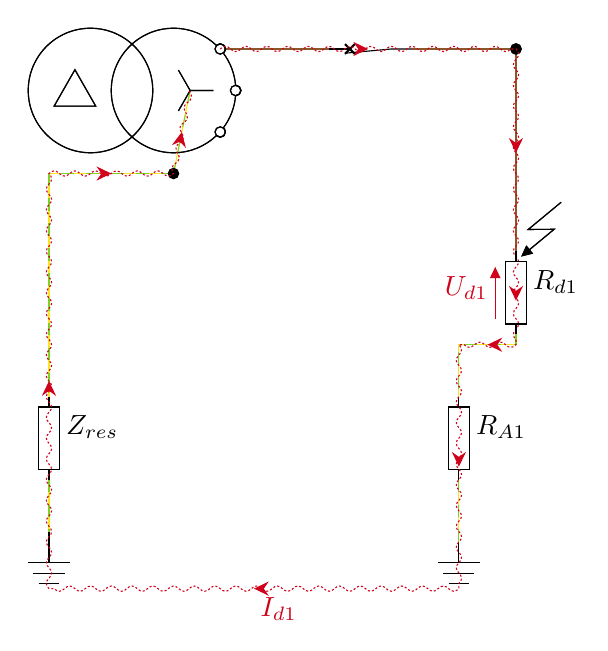
\begin{tikzpicture}[x=0.75pt,y=0.75pt,yscale=-1,xscale=1]
%uncomment if require: \path (0,313); %set diagram left start at 0, and has height of 313

%Straight Lines [id:da40140774002563195] 
\draw [color={rgb, 255:red, 248; green, 231; blue, 28 }  ,draw opacity=1 ]   (87.5,75) -- (27.5,75) -- (27.5,182.5) ;
%Straight Lines [id:da7768656062968136] 
\draw [color={rgb, 255:red, 248; green, 231; blue, 28 }  ,draw opacity=1 ]   (95.5,35) -- (87.5,75) ;
%Straight Lines [id:da0702550211386399] 
\draw [color={rgb, 255:red, 126; green, 211; blue, 33 }  ,draw opacity=1 ] [dash pattern={on 4.5pt off 4.5pt}]  (95.5,35) -- (87.5,75) ;
%Shape: Path Data [id:dp6564394705196642] 
\draw   (112.5,55) .. controls (112.5,56.38) and (111.38,57.5) .. (110,57.5) .. controls (109.29,57.5) and (108.65,57.2) .. (108.19,56.72) .. controls (102.81,61.85) and (95.52,65) .. (87.5,65) .. controls (70.93,65) and (57.5,51.57) .. (57.5,35) .. controls (57.5,18.43) and (70.93,5) .. (87.5,5) .. controls (95.52,5) and (102.81,8.15) .. (108.19,13.28) .. controls (108.65,12.8) and (109.29,12.5) .. (110,12.5) .. controls (111.38,12.5) and (112.5,13.62) .. (112.5,15) .. controls (112.5,15.82) and (112.11,16.54) .. (111.5,17) .. controls (114.8,21.39) and (116.92,26.71) .. (117.4,32.5) .. controls (117.43,32.5) and (117.47,32.5) .. (117.5,32.5) .. controls (118.88,32.5) and (120,33.62) .. (120,35) .. controls (120,36.38) and (118.88,37.5) .. (117.5,37.5) .. controls (117.47,37.5) and (117.43,37.5) .. (117.4,37.5) .. controls (116.92,43.29) and (114.8,48.61) .. (111.5,53) .. controls (112.11,53.46) and (112.5,54.18) .. (112.5,55) -- cycle ;
%Shape: Circle [id:dp6837865910950578] 
\draw   (17.5,35) .. controls (17.5,18.43) and (30.93,5) .. (47.5,5) .. controls (64.07,5) and (77.5,18.43) .. (77.5,35) .. controls (77.5,51.57) and (64.07,65) .. (47.5,65) .. controls (30.93,65) and (17.5,51.57) .. (17.5,35) -- cycle ;
%Shape: Triangle [id:dp4328019700995849] 
\draw   (40,25) -- (30,42.5) -- (50,42.5) -- cycle ;
%Shape: Star [id:dp9996543744584487] 
\draw   (106.75,35) -- (95.5,35) -- (89.88,44.81) -- (95.5,35) -- (89.88,25.19) -- (95.5,35) -- cycle ;
%Shape: Circle [id:dp4765432529475536] 
\draw   (107.5,15) .. controls (107.5,13.62) and (108.62,12.5) .. (110,12.5) .. controls (111.38,12.5) and (112.5,13.62) .. (112.5,15) .. controls (112.5,16.38) and (111.38,17.5) .. (110,17.5) .. controls (108.62,17.5) and (107.5,16.38) .. (107.5,15) -- cycle ;
%Shape: Circle [id:dp7950957606894842] 
\draw   (114.9,35) .. controls (114.9,33.62) and (116.02,32.5) .. (117.4,32.5) .. controls (118.78,32.5) and (119.9,33.62) .. (119.9,35) .. controls (119.9,36.38) and (118.78,37.5) .. (117.4,37.5) .. controls (116.02,37.5) and (114.9,36.38) .. (114.9,35) -- cycle ;
%Shape: Circle [id:dp47024921818209997] 
\draw   (107.5,55) .. controls (107.5,53.62) and (108.62,52.5) .. (110,52.5) .. controls (111.38,52.5) and (112.5,53.62) .. (112.5,55) .. controls (112.5,56.38) and (111.38,57.5) .. (110,57.5) .. controls (108.62,57.5) and (107.5,56.38) .. (107.5,55) -- cycle ;

%Straight Lines [id:da21818556641513764] 
\draw [color={rgb, 255:red, 139; green, 87; blue, 42 }  ,draw opacity=1 ]   (252.5,112.5) -- (252.5,17.5) ;
%Straight Lines [id:da8686907197740312] 
\draw [color={rgb, 255:red, 248; green, 231; blue, 28 }  ,draw opacity=1 ]   (225,222.5) -- (225,247.5) ;
%Straight Lines [id:da4369452606894554] 
\draw    (225,247.5) -- (225,262.5) ;
%Straight Lines [id:da41347797921121543] 
\draw    (215,262.5) -- (235,262.5) ;
%Straight Lines [id:da39005220989882616] 
\draw    (217.5,267.5) -- (232.5,267.5) ;
%Straight Lines [id:da04530437508662333] 
\draw    (220,272.5) -- (230,272.5) ;

%Straight Lines [id:da758878567860916] 
\draw [color={rgb, 255:red, 126; green, 211; blue, 33 }  ,draw opacity=1 ] [dash pattern={on 4.5pt off 4.5pt}]  (225,222.5) -- (225,247.5) ;
%Straight Lines [id:da7282446695874194] 
\draw    (225,217.5) -- (225,222.5) ;
%Shape: Rectangle [id:dp5377265306575283] 
\draw   (230,187.5) -- (230,217.5) -- (220,217.5) -- (220,187.5) -- cycle ;
%Straight Lines [id:da6172743564243196] 
\draw    (225,182.5) -- (225,187.5) ;

%Shape: Circle [id:dp9518184334454515] 
\draw  [fill={rgb, 255:red, 0; green, 0; blue, 0 }  ,fill opacity=1 ] (250,15) .. controls (250,13.62) and (251.12,12.5) .. (252.5,12.5) .. controls (253.88,12.5) and (255,13.62) .. (255,15) .. controls (255,16.38) and (253.88,17.5) .. (252.5,17.5) .. controls (251.12,17.5) and (250,16.38) .. (250,15) -- cycle ;
%Straight Lines [id:da698344453228456] 
\draw [color={rgb, 255:red, 139; green, 87; blue, 42 }  ,draw opacity=1 ]   (112.5,15) -- (162.5,15) ;
%Straight Lines [id:da3888199822065723] 
\draw [color={rgb, 255:red, 126; green, 211; blue, 33 }  ,draw opacity=1 ] [dash pattern={on 4.5pt off 4.5pt}]  (87.5,75) -- (27.5,75) -- (27.5,182.5) ;
%Straight Lines [id:da9929118367256647] 
\draw    (27.5,217.5) -- (27.5,222.5) ;
%Shape: Rectangle [id:dp5522927597315069] 
\draw   (32.5,187.5) -- (32.5,217.5) -- (22.5,217.5) -- (22.5,187.5) -- cycle ;
%Straight Lines [id:da51565112690186] 
\draw    (27.5,182.5) -- (27.5,187.5) ;

%Straight Lines [id:da20200008374801148] 
\draw [color={rgb, 255:red, 248; green, 231; blue, 28 }  ,draw opacity=1 ]   (27.5,222.5) -- (27.5,247.5) ;
%Straight Lines [id:da246860902568655] 
\draw [color={rgb, 255:red, 126; green, 211; blue, 33 }  ,draw opacity=1 ] [dash pattern={on 4.5pt off 4.5pt}]  (27.5,222.5) -- (27.5,247.5) ;
%Straight Lines [id:da8847595831515674] 
\draw    (27.5,247.5) -- (27.5,262.5) ;
%Straight Lines [id:da388525152974063] 
\draw    (17.5,262.5) -- (37.5,262.5) ;
%Straight Lines [id:da5307482611563814] 
\draw    (20,267.5) -- (35,267.5) ;
%Straight Lines [id:da879280977386573] 
\draw    (22.5,272.5) -- (32.5,272.5) ;

%Shape: Circle [id:dp23726887554171172] 
\draw  [fill={rgb, 255:red, 0; green, 0; blue, 0 }  ,fill opacity=1 ] (85,75) .. controls (85,73.62) and (86.12,72.5) .. (87.5,72.5) .. controls (88.88,72.5) and (90,73.62) .. (90,75) .. controls (90,76.38) and (88.88,77.5) .. (87.5,77.5) .. controls (86.12,77.5) and (85,76.38) .. (85,75) -- cycle ;
%Shape: Boxed Line [id:dp0646171917121674] 
\draw    (274.27,88.83) -- (258.39,101.97) -- (270.89,101.86) -- (257.31,113.09) ;
\draw [shift={(255,115)}, rotate = 320.40999999999997] [fill={rgb, 255:red, 0; green, 0; blue, 0 }  ][line width=0.08]  [draw opacity=0] (5.36,-2.57) -- (0,0) -- (5.36,2.57) -- cycle    ;
%Straight Lines [id:da0893199801246688] 
\draw    (170.5,17) -- (192.5,15) -- (202.5,15) ;
%Straight Lines [id:da4465712907894863] 
\draw    (172.5,15) -- (162.5,15) ;
\draw [shift={(172.5,15)}, rotate = 225] [color={rgb, 255:red, 0; green, 0; blue, 0 }  ][line width=0.75]    (-3.35,0) -- (3.35,0)(0,3.35) -- (0,-3.35)   ;

%Straight Lines [id:da6575503286927553] 
\draw [color={rgb, 255:red, 248; green, 231; blue, 28 }  ,draw opacity=1 ]   (252.5,152.5) -- (252.5,157.5) -- (225,157.5) -- (225,182.5) ;
%Straight Lines [id:da4804418012067295] 
\draw [color={rgb, 255:red, 139; green, 87; blue, 42 }  ,draw opacity=1 ]   (112.5,15) -- (162.5,15) ;
%Straight Lines [id:da7896587451085693] 
\draw [color={rgb, 255:red, 139; green, 87; blue, 42 }  ,draw opacity=1 ]   (202.5,15) -- (252.5,15) ;
%Shape: Path Data [id:dp195065302202169] 
\draw   (112.5,55) .. controls (112.5,56.38) and (111.38,57.5) .. (110,57.5) .. controls (109.29,57.5) and (108.65,57.2) .. (108.19,56.72) .. controls (102.81,61.85) and (95.52,65) .. (87.5,65) .. controls (70.93,65) and (57.5,51.57) .. (57.5,35) .. controls (57.5,18.43) and (70.93,5) .. (87.5,5) .. controls (95.52,5) and (102.81,8.15) .. (108.19,13.28) .. controls (108.65,12.8) and (109.29,12.5) .. (110,12.5) .. controls (111.38,12.5) and (112.5,13.62) .. (112.5,15) .. controls (112.5,15.82) and (112.11,16.54) .. (111.5,17) .. controls (114.8,21.39) and (116.92,26.71) .. (117.4,32.5) .. controls (117.43,32.5) and (117.47,32.5) .. (117.5,32.5) .. controls (118.88,32.5) and (120,33.62) .. (120,35) .. controls (120,36.38) and (118.88,37.5) .. (117.5,37.5) .. controls (117.47,37.5) and (117.43,37.5) .. (117.4,37.5) .. controls (116.92,43.29) and (114.8,48.61) .. (111.5,53) .. controls (112.11,53.46) and (112.5,54.18) .. (112.5,55) -- cycle ;
%Shape: Circle [id:dp10449815547230978] 
\draw   (17.5,35) .. controls (17.5,18.43) and (30.93,5) .. (47.5,5) .. controls (64.07,5) and (77.5,18.43) .. (77.5,35) .. controls (77.5,51.57) and (64.07,65) .. (47.5,65) .. controls (30.93,65) and (17.5,51.57) .. (17.5,35) -- cycle ;
%Shape: Triangle [id:dp13602835689186588] 
\draw   (40,25) -- (30,42.5) -- (50,42.5) -- cycle ;
%Shape: Star [id:dp5246434088790826] 
\draw   (106.75,35) -- (95.5,35) -- (89.88,44.81) -- (95.5,35) -- (89.88,25.19) -- (95.5,35) -- cycle ;
%Shape: Circle [id:dp3622486105745091] 
\draw   (107.5,15) .. controls (107.5,13.62) and (108.62,12.5) .. (110,12.5) .. controls (111.38,12.5) and (112.5,13.62) .. (112.5,15) .. controls (112.5,16.38) and (111.38,17.5) .. (110,17.5) .. controls (108.62,17.5) and (107.5,16.38) .. (107.5,15) -- cycle ;
%Shape: Circle [id:dp7116693252528491] 
\draw   (114.9,35) .. controls (114.9,33.62) and (116.02,32.5) .. (117.4,32.5) .. controls (118.78,32.5) and (119.9,33.62) .. (119.9,35) .. controls (119.9,36.38) and (118.78,37.5) .. (117.4,37.5) .. controls (116.02,37.5) and (114.9,36.38) .. (114.9,35) -- cycle ;
%Shape: Circle [id:dp18972999107641209] 
\draw   (107.5,55) .. controls (107.5,53.62) and (108.62,52.5) .. (110,52.5) .. controls (111.38,52.5) and (112.5,53.62) .. (112.5,55) .. controls (112.5,56.38) and (111.38,57.5) .. (110,57.5) .. controls (108.62,57.5) and (107.5,56.38) .. (107.5,55) -- cycle ;

%Straight Lines [id:da014549812099070136] 
\draw [color={rgb, 255:red, 139; green, 87; blue, 42 }  ,draw opacity=1 ]   (252.5,112.5) -- (252.5,17.5) ;
%Straight Lines [id:da26084750256284417] 
\draw [color={rgb, 255:red, 126; green, 211; blue, 33 }  ,draw opacity=1 ] [dash pattern={on 4.5pt off 4.5pt}]  (252.5,152.5) -- (252.5,157.5) -- (225,157.5) -- (225,182.5) ;
%Straight Lines [id:da3030992302203893] 
\draw [color={rgb, 255:red, 248; green, 231; blue, 28 }  ,draw opacity=1 ]   (225,222.5) -- (225,252.5) ;
%Straight Lines [id:da15920917753755837] 
\draw [color={rgb, 255:red, 126; green, 211; blue, 33 }  ,draw opacity=1 ] [dash pattern={on 4.5pt off 4.5pt}]  (225,222.5) -- (225,252.5) ;
%Shape: Circle [id:dp17133751283477605] 
\draw  [fill={rgb, 255:red, 0; green, 0; blue, 0 }  ,fill opacity=1 ] (250,15) .. controls (250,13.62) and (251.12,12.5) .. (252.5,12.5) .. controls (253.88,12.5) and (255,13.62) .. (255,15) .. controls (255,16.38) and (253.88,17.5) .. (252.5,17.5) .. controls (251.12,17.5) and (250,16.38) .. (250,15) -- cycle ;
%Shape: Boxed Line [id:dp8068084114642486] 
\draw    (274.27,88.83) -- (258.39,101.97) -- (270.89,101.86) -- (257.31,113.09) ;
\draw [shift={(255,115)}, rotate = 320.40999999999997] [fill={rgb, 255:red, 0; green, 0; blue, 0 }  ][line width=0.08]  [draw opacity=0] (5.36,-2.57) -- (0,0) -- (5.36,2.57) -- cycle    ;
%Straight Lines [id:da21551575051470273] 
\draw [color={rgb, 255:red, 208; green, 2; blue, 27 }  ,draw opacity=1 ] [dash pattern={on 0.75pt off 0.75pt}]  (110,15) .. controls (111.67,13.33) and (113.33,13.33) .. (115,15) .. controls (116.67,16.67) and (118.33,16.67) .. (120,15) .. controls (121.67,13.33) and (123.33,13.33) .. (125,15) .. controls (126.67,16.67) and (128.33,16.67) .. (130,15) .. controls (131.67,13.33) and (133.33,13.33) .. (135,15) .. controls (136.67,16.67) and (138.33,16.67) .. (140,15) .. controls (141.67,13.33) and (143.33,13.33) .. (145,15) .. controls (146.67,16.67) and (148.33,16.67) .. (150,15) .. controls (151.67,13.33) and (153.33,13.33) .. (155,15) .. controls (156.67,16.67) and (158.33,16.67) .. (160,15) .. controls (161.67,13.33) and (163.33,13.33) .. (165,15) .. controls (166.67,16.67) and (168.33,16.67) .. (170,15) .. controls (171.67,13.33) and (173.33,13.33) .. (175,15) .. controls (176.67,16.67) and (178.33,16.67) .. (180,15) .. controls (181.67,13.33) and (183.33,13.33) .. (185,15) .. controls (186.67,16.67) and (188.33,16.67) .. (190,15) .. controls (191.67,13.33) and (193.33,13.33) .. (195,15) .. controls (196.67,16.67) and (198.33,16.67) .. (200,15) .. controls (201.67,13.33) and (203.33,13.33) .. (205,15) .. controls (206.67,16.67) and (208.33,16.67) .. (210,15) .. controls (211.67,13.33) and (213.33,13.33) .. (215,15) .. controls (216.67,16.67) and (218.33,16.67) .. (220,15) .. controls (221.67,13.33) and (223.33,13.33) .. (225,15) .. controls (226.67,16.67) and (228.33,16.67) .. (230,15) .. controls (231.67,13.33) and (233.33,13.33) .. (235,15) .. controls (236.67,16.67) and (238.33,16.67) .. (240,15) .. controls (241.67,13.33) and (243.33,13.33) .. (245,15) .. controls (246.67,16.67) and (248.33,16.67) .. (250,15) -- (252.5,15) -- (252.5,15) .. controls (254.17,16.67) and (254.17,18.33) .. (252.5,20) .. controls (250.83,21.67) and (250.83,23.33) .. (252.5,25) .. controls (254.17,26.67) and (254.17,28.33) .. (252.5,30) .. controls (250.83,31.67) and (250.83,33.33) .. (252.5,35) .. controls (254.17,36.67) and (254.17,38.33) .. (252.5,40) .. controls (250.83,41.67) and (250.83,43.33) .. (252.5,45) .. controls (254.17,46.67) and (254.17,48.33) .. (252.5,50) .. controls (250.83,51.67) and (250.83,53.33) .. (252.5,55) .. controls (254.17,56.67) and (254.17,58.33) .. (252.5,60) .. controls (250.83,61.67) and (250.83,63.33) .. (252.5,65) .. controls (254.17,66.67) and (254.17,68.33) .. (252.5,70) .. controls (250.83,71.67) and (250.83,73.33) .. (252.5,75) .. controls (254.17,76.67) and (254.17,78.33) .. (252.5,80) .. controls (250.83,81.67) and (250.83,83.33) .. (252.5,85) .. controls (254.17,86.67) and (254.17,88.33) .. (252.5,90) .. controls (250.83,91.67) and (250.83,93.33) .. (252.5,95) .. controls (254.17,96.67) and (254.17,98.33) .. (252.5,100) .. controls (250.83,101.67) and (250.83,103.33) .. (252.5,105) .. controls (254.17,106.67) and (254.17,108.33) .. (252.5,110) .. controls (250.83,111.67) and (250.83,113.33) .. (252.5,115) -- (252.5,115) .. controls (254.17,116.67) and (254.17,118.33) .. (252.5,120) .. controls (250.83,121.67) and (250.83,123.33) .. (252.5,125) .. controls (254.17,126.67) and (254.17,128.33) .. (252.5,130) .. controls (250.83,131.67) and (250.83,133.33) .. (252.5,135) .. controls (254.17,136.67) and (254.17,138.33) .. (252.5,140) .. controls (250.83,141.67) and (250.83,143.33) .. (252.5,145) .. controls (254.17,146.67) and (254.17,148.33) .. (252.5,150) .. controls (250.83,151.67) and (250.83,153.33) .. (252.5,155) -- (252.5,157.5) -- (252.5,157.5) .. controls (250.83,159.17) and (249.17,159.17) .. (247.5,157.5) .. controls (245.83,155.83) and (244.17,155.83) .. (242.5,157.5) .. controls (240.83,159.17) and (239.17,159.17) .. (237.5,157.5) .. controls (235.83,155.83) and (234.17,155.83) .. (232.5,157.5) .. controls (230.83,159.17) and (229.17,159.17) .. (227.5,157.5) -- (225,157.5) -- (225,157.5) .. controls (226.67,159.17) and (226.67,160.83) .. (225,162.5) .. controls (223.33,164.17) and (223.33,165.83) .. (225,167.5) .. controls (226.67,169.17) and (226.67,170.83) .. (225,172.5) .. controls (223.33,174.17) and (223.33,175.83) .. (225,177.5) .. controls (226.67,179.17) and (226.67,180.83) .. (225,182.5) .. controls (223.33,184.17) and (223.33,185.83) .. (225,187.5) .. controls (226.67,189.17) and (226.67,190.83) .. (225,192.5) .. controls (223.33,194.17) and (223.33,195.83) .. (225,197.5) .. controls (226.67,199.17) and (226.67,200.83) .. (225,202.5) .. controls (223.33,204.17) and (223.33,205.83) .. (225,207.5) .. controls (226.67,209.17) and (226.67,210.83) .. (225,212.5) .. controls (223.33,214.17) and (223.33,215.83) .. (225,217.5) .. controls (226.67,219.17) and (226.67,220.83) .. (225,222.5) .. controls (223.33,224.17) and (223.33,225.83) .. (225,227.5) .. controls (226.67,229.17) and (226.67,230.83) .. (225,232.5) .. controls (223.33,234.17) and (223.33,235.83) .. (225,237.5) .. controls (226.67,239.17) and (226.67,240.83) .. (225,242.5) .. controls (223.33,244.17) and (223.33,245.83) .. (225,247.5) .. controls (226.67,249.17) and (226.67,250.83) .. (225,252.5) .. controls (223.33,254.17) and (223.33,255.83) .. (225,257.5) .. controls (226.67,259.17) and (226.67,260.83) .. (225,262.5) .. controls (223.33,264.17) and (223.33,265.83) .. (225,267.5) .. controls (226.67,269.17) and (226.67,270.83) .. (225,272.5) -- (225,275) -- (225,275) .. controls (223.33,276.67) and (221.67,276.67) .. (220,275) .. controls (218.33,273.33) and (216.67,273.33) .. (215,275) .. controls (213.33,276.67) and (211.67,276.67) .. (210,275) .. controls (208.33,273.33) and (206.67,273.33) .. (205,275) .. controls (203.33,276.67) and (201.67,276.67) .. (200,275) .. controls (198.33,273.33) and (196.67,273.33) .. (195,275) .. controls (193.33,276.67) and (191.67,276.67) .. (190,275) .. controls (188.33,273.33) and (186.67,273.33) .. (185,275) .. controls (183.33,276.67) and (181.67,276.67) .. (180,275) .. controls (178.33,273.33) and (176.67,273.33) .. (175,275) .. controls (173.33,276.67) and (171.67,276.67) .. (170,275) .. controls (168.33,273.33) and (166.67,273.33) .. (165,275) .. controls (163.33,276.67) and (161.67,276.67) .. (160,275) .. controls (158.33,273.33) and (156.67,273.33) .. (155,275) .. controls (153.33,276.67) and (151.67,276.67) .. (150,275) .. controls (148.33,273.33) and (146.67,273.33) .. (145,275) .. controls (143.33,276.67) and (141.67,276.67) .. (140,275) .. controls (138.33,273.33) and (136.67,273.33) .. (135,275) .. controls (133.33,276.67) and (131.67,276.67) .. (130,275) .. controls (128.33,273.33) and (126.67,273.33) .. (125,275) .. controls (123.33,276.67) and (121.67,276.67) .. (120,275) .. controls (118.33,273.33) and (116.67,273.33) .. (115,275) .. controls (113.33,276.67) and (111.67,276.67) .. (110,275) .. controls (108.33,273.33) and (106.67,273.33) .. (105,275) .. controls (103.33,276.67) and (101.67,276.67) .. (100,275) .. controls (98.33,273.33) and (96.67,273.33) .. (95,275) .. controls (93.33,276.67) and (91.67,276.67) .. (90,275) .. controls (88.33,273.33) and (86.67,273.33) .. (85,275) .. controls (83.33,276.67) and (81.67,276.67) .. (80,275) .. controls (78.33,273.33) and (76.67,273.33) .. (75,275) .. controls (73.33,276.67) and (71.67,276.67) .. (70,275) .. controls (68.33,273.33) and (66.67,273.33) .. (65,275) .. controls (63.33,276.67) and (61.67,276.67) .. (60,275) .. controls (58.33,273.33) and (56.67,273.33) .. (55,275) .. controls (53.33,276.67) and (51.67,276.67) .. (50,275) .. controls (48.33,273.33) and (46.67,273.33) .. (45,275) .. controls (43.33,276.67) and (41.67,276.67) .. (40,275) .. controls (38.33,273.33) and (36.67,273.33) .. (35,275) .. controls (33.33,276.67) and (31.67,276.67) .. (30,275) -- (27.5,275) -- (27.5,275) .. controls (25.83,273.33) and (25.83,271.67) .. (27.5,270) .. controls (29.17,268.33) and (29.17,266.67) .. (27.5,265) .. controls (25.83,263.33) and (25.83,261.67) .. (27.5,260) .. controls (29.17,258.33) and (29.17,256.67) .. (27.5,255) .. controls (25.83,253.33) and (25.83,251.67) .. (27.5,250) .. controls (29.17,248.33) and (29.17,246.67) .. (27.5,245) .. controls (25.83,243.33) and (25.83,241.67) .. (27.5,240) .. controls (29.17,238.33) and (29.17,236.67) .. (27.5,235) .. controls (25.83,233.33) and (25.83,231.67) .. (27.5,230) .. controls (29.17,228.33) and (29.17,226.67) .. (27.5,225) .. controls (25.83,223.33) and (25.83,221.67) .. (27.5,220) .. controls (29.17,218.33) and (29.17,216.67) .. (27.5,215) .. controls (25.83,213.33) and (25.83,211.67) .. (27.5,210) .. controls (29.17,208.33) and (29.17,206.67) .. (27.5,205) .. controls (25.83,203.33) and (25.83,201.67) .. (27.5,200) .. controls (29.17,198.33) and (29.17,196.67) .. (27.5,195) .. controls (25.83,193.33) and (25.83,191.67) .. (27.5,190) .. controls (29.17,188.33) and (29.17,186.67) .. (27.5,185) .. controls (25.83,183.33) and (25.83,181.67) .. (27.5,180) .. controls (29.17,178.33) and (29.17,176.67) .. (27.5,175) .. controls (25.83,173.33) and (25.83,171.67) .. (27.5,170) .. controls (29.17,168.33) and (29.17,166.67) .. (27.5,165) .. controls (25.83,163.33) and (25.83,161.67) .. (27.5,160) .. controls (29.17,158.33) and (29.17,156.67) .. (27.5,155) .. controls (25.83,153.33) and (25.83,151.67) .. (27.5,150) .. controls (29.17,148.33) and (29.17,146.67) .. (27.5,145) .. controls (25.83,143.33) and (25.83,141.67) .. (27.5,140) .. controls (29.17,138.33) and (29.17,136.67) .. (27.5,135) .. controls (25.83,133.33) and (25.83,131.67) .. (27.5,130) .. controls (29.17,128.33) and (29.17,126.67) .. (27.5,125) .. controls (25.83,123.33) and (25.83,121.67) .. (27.5,120) .. controls (29.17,118.33) and (29.17,116.67) .. (27.5,115) .. controls (25.83,113.33) and (25.83,111.67) .. (27.5,110) .. controls (29.17,108.33) and (29.17,106.67) .. (27.5,105) .. controls (25.83,103.33) and (25.83,101.67) .. (27.5,100) .. controls (29.17,98.33) and (29.17,96.67) .. (27.5,95) .. controls (25.83,93.33) and (25.83,91.67) .. (27.5,90) .. controls (29.17,88.33) and (29.17,86.67) .. (27.5,85) .. controls (25.83,83.33) and (25.83,81.67) .. (27.5,80) .. controls (29.17,78.33) and (29.17,76.67) .. (27.5,75) -- (27.5,75) .. controls (29.17,73.33) and (30.83,73.33) .. (32.5,75) .. controls (34.17,76.67) and (35.83,76.67) .. (37.5,75) .. controls (39.17,73.33) and (40.83,73.33) .. (42.5,75) .. controls (44.17,76.67) and (45.83,76.67) .. (47.5,75) .. controls (49.17,73.33) and (50.83,73.33) .. (52.5,75) .. controls (54.17,76.67) and (55.83,76.67) .. (57.5,75) .. controls (59.17,73.33) and (60.83,73.33) .. (62.5,75) .. controls (64.17,76.67) and (65.83,76.67) .. (67.5,75) .. controls (69.17,73.33) and (70.83,73.33) .. (72.5,75) .. controls (74.17,76.67) and (75.83,76.67) .. (77.5,75) .. controls (79.17,73.33) and (80.83,73.33) .. (82.5,75) .. controls (84.17,76.67) and (85.83,76.67) .. (87.5,75) -- (87.5,75) .. controls (86.19,73.04) and (86.52,71.41) .. (88.48,70.1) .. controls (90.44,68.79) and (90.77,67.15) .. (89.46,65.19) .. controls (88.15,63.23) and (88.48,61.6) .. (90.44,60.29) .. controls (92.4,58.98) and (92.73,57.35) .. (91.42,55.39) .. controls (90.11,53.43) and (90.44,51.8) .. (92.4,50.49) .. controls (94.36,49.18) and (94.69,47.54) .. (93.38,45.58) .. controls (92.07,43.62) and (92.4,41.99) .. (94.36,40.68) .. controls (96.32,39.37) and (96.65,37.74) .. (95.34,35.78) -- (95.5,35) -- (95.5,35) ;
\draw [shift={(181.25,15)}, rotate = 180] [fill={rgb, 255:red, 208; green, 2; blue, 27 }  ,fill opacity=1 ][line width=0.08]  [draw opacity=0] (7.14,-3.43) -- (0,0) -- (7.14,3.43) -- (4.74,0) -- cycle    ;
\draw [shift={(252.5,65)}, rotate = 270] [fill={rgb, 255:red, 208; green, 2; blue, 27 }  ,fill opacity=1 ][line width=0.08]  [draw opacity=0] (7.14,-3.43) -- (0,0) -- (7.14,3.43) -- (4.74,0) -- cycle    ;
\draw [shift={(252.5,136.25)}, rotate = 270] [fill={rgb, 255:red, 208; green, 2; blue, 27 }  ,fill opacity=1 ][line width=0.08]  [draw opacity=0] (7.14,-3.43) -- (0,0) -- (7.14,3.43) -- (4.74,0) -- cycle    ;
\draw [shift={(238.75,157.5)}, rotate = 360] [fill={rgb, 255:red, 208; green, 2; blue, 27 }  ,fill opacity=1 ][line width=0.08]  [draw opacity=0] (7.14,-3.43) -- (0,0) -- (7.14,3.43) -- (4.74,0) -- cycle    ;
\draw [shift={(225,216.25)}, rotate = 270] [fill={rgb, 255:red, 208; green, 2; blue, 27 }  ,fill opacity=1 ][line width=0.08]  [draw opacity=0] (7.14,-3.43) -- (0,0) -- (7.14,3.43) -- (4.74,0) -- cycle    ;
\draw [shift={(126.25,275)}, rotate = 360] [fill={rgb, 255:red, 208; green, 2; blue, 27 }  ,fill opacity=1 ][line width=0.08]  [draw opacity=0] (7.14,-3.43) -- (0,0) -- (7.14,3.43) -- (4.74,0) -- cycle    ;
\draw [shift={(27.5,175)}, rotate = 450] [fill={rgb, 255:red, 208; green, 2; blue, 27 }  ,fill opacity=1 ][line width=0.08]  [draw opacity=0] (7.14,-3.43) -- (0,0) -- (7.14,3.43) -- (4.74,0) -- cycle    ;
\draw [shift={(57.5,75)}, rotate = 180] [fill={rgb, 255:red, 208; green, 2; blue, 27 }  ,fill opacity=1 ][line width=0.08]  [draw opacity=0] (7.14,-3.43) -- (0,0) -- (7.14,3.43) -- (4.74,0) -- cycle    ;
\draw [shift={(91.5,55)}, rotate = 461.31] [fill={rgb, 255:red, 208; green, 2; blue, 27 }  ,fill opacity=1 ][line width=0.08]  [draw opacity=0] (7.14,-3.43) -- (0,0) -- (7.14,3.43) -- (4.74,0) -- cycle    ;
%Straight Lines [id:da5878987587379367] 
\draw    (252.5,147.5) -- (252.5,152.5) ;
%Shape: Rectangle [id:dp5233395725568003] 
\draw   (257.5,117.5) -- (257.5,147.5) -- (247.5,147.5) -- (247.5,117.5) -- cycle ;
%Straight Lines [id:da6884797067797518] 
\draw    (252.5,112.5) -- (252.5,117.5) ;

%Straight Lines [id:da07071854927031873] 
\draw [color={rgb, 255:red, 208; green, 2; blue, 27 }  ,draw opacity=1 ]   (242.5,123) -- (242.5,145) ;
\draw [shift={(242.5,120)}, rotate = 90] [fill={rgb, 255:red, 208; green, 2; blue, 27 }  ,fill opacity=1 ][line width=0.08]  [draw opacity=0] (5.36,-2.57) -- (0,0) -- (5.36,2.57) -- cycle    ;

% Text Node
\draw (232,190.5) node [anchor=north west][inner sep=0.75pt]   [align=left] {$R_{A1}$};
% Text Node
\draw (34.5,190.5) node [anchor=north west][inner sep=0.75pt]   [align=left] {$Z_{res}$};
% Text Node
\draw (128.25,278) node [anchor=north west][inner sep=0.75pt]  [color={rgb, 255:red, 208; green, 2; blue, 27 }  ,opacity=1 ] [align=left] {$I_{d1}$};
% Text Node
\draw (217,123.5) node [anchor=north west][inner sep=0.75pt]  [color={rgb, 255:red, 208; green, 2; blue, 27 }  ,opacity=1 ] [align=left] {$U_{d1}$};
% Text Node
\draw (259.5,120.5) node [anchor=north west][inner sep=0.75pt]   [align=left] {$R_{d1}$};


\end{tikzpicture}
\end{figure}

%\end{document}


L'intensité de courant $I_d1$ vaut alors :
\begin{formule}{Courant du premier défaut $I_d1$ en schéma Isolé-Individuel}{}
\begin{align*}
		I_d &= \frac{U_{0}}{Z_{res}+R_{A1}+R_{d1}}
\end{align*}

\begin{textvariables}
U_{0}						& tension nominale simple						& volt			& \volt					& 	Différence de potentiel entre les masses métalliques et la terre 	\\
Z_{res}						& impédance											& ohm			& \ohm					& 	Impédance de fuite $Z_res$ du réseau électrique 	\\
R_{A1}						& résistance											& ohm			& \ohm					& 	Résistance de la prise de terre de l'appareil 1 	\\
R_{d1}						& résistance											& ohm			& \ohm					& 	Résistance de défaut 	d'isolement de l'appareil 1\\
\end{textvariables}
\end{formule}

Le courant de défaut $I_{d1}$ fera alors apparaître une \emph{tension de défaut} $U_{d1}$ entre la masse métallique de l'appareil 1 et la terre. Cette tension, limitée par l'impédance de fuite, sera très largement inférieure à  $U_L$ et ne sera donc pas dangereuse. La situation sera similaire avec un schéma Impédant-Individuel $Z_N$, ou l'impédance de limitation limitera également le courant de défaut :

\begin{formule}{Tension de défaut $U_{d1}$ en schéma Isolé-Individuel}{}
\begin{align*}
		U_{d1} &= R_{A1} \times I_{d1} \\
			   &\ll	 U_L
\end{align*}

\begin{textvariables}
R_{A1}						& résistance											& ohm			& \ohm					& 	Résistance de la prise de terre de l'appareil 1 	\\
I_{d1}							& intensité							& ampère		& \ampere				& 	Courant de défaut de l'appareil 1\\
U_{L}						& tension							& volt			& \volt					& 	Tension de sécurité du local avec :
\begin{description}[nosep, leftmargin=*]
\item[Local sec :] $U_{L}=\SI{50}{\volt}$
\item[Local humide :] $U_{L}=\SI{25}{\volt}$
\end{description} \\
\end{textvariables}
\end{formule}

Le fonctionnement d'un schéma IT sera également identique au premier défaut, que les masses soient interconnectées ou individuellement raccordées à la terre.

\begin{exemple}{Tension de défaut $U_{d1}$ en schéma Isolé-Individuel au premier défaut}{}
Si on considère que le transformateur est un transformateur $\SI{20}{\kilo\volt}/\SI{400}{\volt}$, que $Z_{res}=\SI{3500}{\ohm}$, $R_{A1}=\SI{40}{\ohm}$ et que $R_d = \SI{2}{\ohm}$, on peut déduire que le courant de défaut $I_d$ vaut :
\begin{align*}
		I_{d1} &= \frac{U_{0}}{Z_{res}+R_{A1}+R_{d1}} \\
				&=\frac{400}{3500+40+2} \\
				&= \SI{64,9}{\milli\ampere} \\
\end{align*}
Si une personne touche à la masse du récepteur 1, elle sera soumise à une tension de défaut $U_{d1}$ :
\begin{align*}
		U_{d1} &= R_{A1} \times I_{d1} \\
				&=40 \times 0,0649 \\
				&= \SI{2,6}{\volt}
\end{align*}
\end{exemple}

Lors de l'apparition d'un deuxième défaut d'isolement sur un autre conducteur actif, un courant de défaut $I_{d2}$ va apparaitre. Celui-ci va s'apparenter à un court-circuit et de ce fait, $I_{d1}$ sera négligé. \\
Dans les calculs, il faut encore tenir compte de la \emph{résistance de défaut} $R_d$ qui prend en compte la nature du défaut d'isolement (franc ou non-franc) et les résistances des carcasses métalliques des appareils 1 et 2.\\

\begin{figure}[H]
\caption{Installation Isolé-Individuelle}
\begin{subfigure}[t]{0.49\linewidth}
%--------------------------------------
%ELECTROTECHNIQUE - SCHEMA DE LIAISON A LA TERRE
%--------------------------------------

%utiliser les environnement \begin{comment} \end{comment} pour mettre en commentaire le préambule une fois la programmation appelée dans le document maître (!ne pas oublier de mettre en commentaire \end{document}!)

\begin{comment}

\documentclass[a4paper, 11pt, twoside, fleqn]{memoir}

\usepackage{AOCDTF}

\marqueurchapitre
\decoupagechapitre{1} %juste pour éviter les erreurs lors de la compilation des sous-programmations (passera en commentaire)

%lien d'édition des figures Tikz sur le site mathcha.io (rajouter le lien d'une modification effectuée sur la figure tikz avec le nom du modificateur car il n'y a qu'un lien par compte)

%lien mathcha Bruno Douchy : https://www.mathcha.io/editor/DXXG1FgjiNJCe0yo2ZTqzEeM8hlg57ygtvk5Mpy

%--------------------------------------
%corps du document
%--------------------------------------

\begin{document} %corps du document
	\openleft %début de chapitre à gauche

\end{comment}


% Pattern Info
 
\tikzset{
pattern size/.store in=\mcSize, 
pattern size = 5pt,
pattern thickness/.store in=\mcThickness, 
pattern thickness = 0.3pt,
pattern radius/.store in=\mcRadius, 
pattern radius = 1pt}
\makeatletter
\pgfutil@ifundefined{pgf@pattern@name@_ynwbix4sg}{
\pgfdeclarepatternformonly[\mcThickness,\mcSize]{_ynwbix4sg}
{\pgfqpoint{0pt}{0pt}}
{\pgfpoint{\mcSize+\mcThickness}{\mcSize+\mcThickness}}
{\pgfpoint{\mcSize}{\mcSize}}
{
\pgfsetcolor{\tikz@pattern@color}
\pgfsetlinewidth{\mcThickness}
\pgfpathmoveto{\pgfqpoint{0pt}{0pt}}
\pgfpathlineto{\pgfpoint{\mcSize+\mcThickness}{\mcSize+\mcThickness}}
\pgfusepath{stroke}
}}
\makeatother
\tikzset{every picture/.style={line width=0.5pt}} %set default line width to 0.75pt        

\begin{tikzpicture}[x=0.75pt,y=0.75pt,yscale=-0.6,xscale=0.6]
%uncomment if require: \path (0,293); %set diagram left start at 0, and has height of 293

%Shape: Rectangle [id:dp7263765394963575] 
\draw  [dash pattern={on 2.25pt off 2.25pt on 1pt off 2.25pt}] (242.5,115) -- (302.5,115) -- (302.5,145) -- (242.5,145) -- cycle ;
%Shape: Rectangle [id:dp35881098160444513] 
\draw  [dash pattern={on 2.25pt off 2.25pt on 1pt off 2.25pt}] (327.5,115) -- (387.5,115) -- (387.5,145) -- (327.5,145) -- cycle ;
%Shape: Rectangle [id:dp6695507085328443] 
\draw  [dash pattern={on 2.25pt off 2.25pt on 1pt off 2.25pt}] (412.5,115) -- (472.5,115) -- (472.5,145) -- (412.5,145) -- cycle ;
%Straight Lines [id:da8040415491242667] 
\draw [color={rgb, 255:red, 74; green, 144; blue, 226 }  ,draw opacity=1 ]   (90,75) -- (162.5,75) ;
%Straight Lines [id:da39577632473002744] 
\draw [color={rgb, 255:red, 74; green, 144; blue, 226 }  ,draw opacity=1 ]   (202.5,75.5) -- (460,75) ;
%Straight Lines [id:da25678520536510285] 
\draw [color={rgb, 255:red, 248; green, 231; blue, 28 }  ,draw opacity=1 ]   (87.5,75) -- (27.5,75) -- (27.5,182.5) ;
%Straight Lines [id:da5402140347093166] 
\draw [color={rgb, 255:red, 248; green, 231; blue, 28 }  ,draw opacity=1 ]   (95.5,35) -- (87.5,75) -- (87.5,107.5) ;
%Straight Lines [id:da6572902402425455] 
\draw [color={rgb, 255:red, 126; green, 211; blue, 33 }  ,draw opacity=1 ] [dash pattern={on 2.25pt off 2.25pt}]  (95.5,35) -- (87.5,75) -- (87.5,107.5) ;
%Straight Lines [id:da06818694087843613] 
\draw [color={rgb, 255:red, 248; green, 231; blue, 28 }  ,draw opacity=1 ]   (240,135) -- (225,135) -- (225,182.5) ;
%Straight Lines [id:da43234765426393074] 
\draw    (202.5,35) -- (462.5,35) ;
%Straight Lines [id:da8191173199817187] 
\draw [color={rgb, 255:red, 139; green, 87; blue, 42 }  ,draw opacity=1 ]   (202.5,15) -- (462.5,15) ;
%Straight Lines [id:da3978846646736923] 
\draw [color={rgb, 255:red, 155; green, 155; blue, 155 }  ,draw opacity=1 ]   (202.5,55) -- (462.5,55) ;
%Shape: Path Data [id:dp12879159047606914] 
\draw   (112.5,55) .. controls (112.5,56.38) and (111.38,57.5) .. (110,57.5) .. controls (109.29,57.5) and (108.65,57.2) .. (108.19,56.72) .. controls (102.81,61.85) and (95.52,65) .. (87.5,65) .. controls (70.93,65) and (57.5,51.57) .. (57.5,35) .. controls (57.5,18.43) and (70.93,5) .. (87.5,5) .. controls (95.52,5) and (102.81,8.15) .. (108.19,13.28) .. controls (108.65,12.8) and (109.29,12.5) .. (110,12.5) .. controls (111.38,12.5) and (112.5,13.62) .. (112.5,15) .. controls (112.5,15.82) and (112.11,16.54) .. (111.5,17) .. controls (114.8,21.39) and (116.92,26.71) .. (117.4,32.5) .. controls (117.43,32.5) and (117.47,32.5) .. (117.5,32.5) .. controls (118.88,32.5) and (120,33.62) .. (120,35) .. controls (120,36.38) and (118.88,37.5) .. (117.5,37.5) .. controls (117.47,37.5) and (117.43,37.5) .. (117.4,37.5) .. controls (116.92,43.29) and (114.8,48.61) .. (111.5,53) .. controls (112.11,53.46) and (112.5,54.18) .. (112.5,55) -- cycle ;
%Shape: Circle [id:dp3480809900403856] 
\draw   (17.5,35) .. controls (17.5,18.43) and (30.93,5) .. (47.5,5) .. controls (64.07,5) and (77.5,18.43) .. (77.5,35) .. controls (77.5,51.57) and (64.07,65) .. (47.5,65) .. controls (30.93,65) and (17.5,51.57) .. (17.5,35) -- cycle ;
%Shape: Triangle [id:dp8604762228071411] 
\draw   (40,25) -- (30,42.5) -- (50,42.5) -- cycle ;
%Shape: Star [id:dp8212895262481444] 
\draw   (106.75,35) -- (95.5,35) -- (89.88,44.81) -- (95.5,35) -- (89.88,25.19) -- (95.5,35) -- cycle ;
%Shape: Circle [id:dp6479761831984828] 
\draw   (107.5,15) .. controls (107.5,13.62) and (108.62,12.5) .. (110,12.5) .. controls (111.38,12.5) and (112.5,13.62) .. (112.5,15) .. controls (112.5,16.38) and (111.38,17.5) .. (110,17.5) .. controls (108.62,17.5) and (107.5,16.38) .. (107.5,15) -- cycle ;
%Shape: Circle [id:dp9340435311488099] 
\draw   (114.9,35) .. controls (114.9,33.62) and (116.02,32.5) .. (117.4,32.5) .. controls (118.78,32.5) and (119.9,33.62) .. (119.9,35) .. controls (119.9,36.38) and (118.78,37.5) .. (117.4,37.5) .. controls (116.02,37.5) and (114.9,36.38) .. (114.9,35) -- cycle ;
%Shape: Circle [id:dp10166063766932587] 
\draw   (107.5,55) .. controls (107.5,53.62) and (108.62,52.5) .. (110,52.5) .. controls (111.38,52.5) and (112.5,53.62) .. (112.5,55) .. controls (112.5,56.38) and (111.38,57.5) .. (110,57.5) .. controls (108.62,57.5) and (107.5,56.38) .. (107.5,55) -- cycle ;

%Straight Lines [id:da06376724385214627] 
\draw [color={rgb, 255:red, 74; green, 144; blue, 226 }  ,draw opacity=1 ]   (292.5,127.5) -- (292.5,77.5) ;
%Straight Lines [id:da722018804938358] 
\draw [color={rgb, 255:red, 139; green, 87; blue, 42 }  ,draw opacity=1 ]   (252.5,127.5) -- (252.5,17.5) ;
%Straight Lines [id:da04125979948539271] 
\draw [color={rgb, 255:red, 139; green, 87; blue, 42 }  ,draw opacity=1 ]   (252.5,130) -- (252.5,117.5) ;
%Straight Lines [id:da12167383062526271] 
\draw [color={rgb, 255:red, 74; green, 144; blue, 226 }  ,draw opacity=1 ]   (292.5,130.5) -- (292.5,117.5) ;
%Straight Lines [id:da4439455248375477] 
\draw    (17.5,232.5) -- (460,232.5) ;
%Shape: Rectangle [id:dp26004049605098345] 
\draw  [draw opacity=0][pattern=_ynwbix4sg,pattern size=6pt,pattern thickness=0.75pt,pattern radius=0pt, pattern color={rgb, 255:red, 0; green, 0; blue, 0}][line width=0.75]  (17.5,232.5) -- (460,232.5) -- (460,247.5) -- (17.5,247.5) -- cycle ;
%Straight Lines [id:da8060373055516235] 
\draw [color={rgb, 255:red, 126; green, 211; blue, 33 }  ,draw opacity=1 ] [dash pattern={on 2.25pt off 2.25pt}]  (240,135) -- (225,135) -- (225,182.5) ;
%Straight Lines [id:da4749821159228028] 
\draw [color={rgb, 255:red, 248; green, 231; blue, 28 }  ,draw opacity=1 ]   (225,222.5) -- (225,247.5) ;
%Straight Lines [id:da062203575977509695] 
\draw    (225,247.5) -- (225,262.5) ;
%Straight Lines [id:da6853805401356492] 
\draw    (215,262.5) -- (235,262.5) ;
%Straight Lines [id:da9659418909077957] 
\draw    (217.5,267.5) -- (232.5,267.5) ;
%Straight Lines [id:da3426588435166359] 
\draw    (220,272.5) -- (230,272.5) ;

%Straight Lines [id:da5066053579270585] 
\draw [color={rgb, 255:red, 126; green, 211; blue, 33 }  ,draw opacity=1 ] [dash pattern={on 2.25pt off 2.25pt}]  (225,222.5) -- (225,247.5) ;
%Straight Lines [id:da8048473053801423] 
\draw    (287.5,130) -- (292.5,130) ;
%Shape: Rectangle [id:dp6961402768131659] 
\draw   (257.5,125) -- (287.5,125) -- (287.5,135) -- (257.5,135) -- cycle ;
%Straight Lines [id:da31174793777370724] 
\draw    (252.5,130) -- (257.5,130) ;

%Straight Lines [id:da16092896219567276] 
\draw    (225,217.5) -- (225,222.5) ;
%Shape: Rectangle [id:dp6821599487691122] 
\draw   (230,187.5) -- (230,217.5) -- (220,217.5) -- (220,187.5) -- cycle ;
%Straight Lines [id:da5392367850767137] 
\draw    (225,182.5) -- (225,187.5) ;

%Straight Lines [id:da6284193535082088] 
\draw [color={rgb, 255:red, 74; green, 144; blue, 226 }  ,draw opacity=1 ]   (377.5,127.5) -- (377.5,77.5) ;
%Straight Lines [id:da8589416903630054] 
\draw [color={rgb, 255:red, 0; green, 0; blue, 0 }  ,draw opacity=1 ]   (337.5,127.5) -- (337.5,37.5) ;
%Straight Lines [id:da44587915586028104] 
\draw [color={rgb, 255:red, 74; green, 144; blue, 226 }  ,draw opacity=1 ]   (377.5,130.5) -- (377.5,117.5) ;
%Straight Lines [id:da3274388544893425] 
\draw    (372.5,130) -- (377.5,130) ;
%Shape: Rectangle [id:dp9931264333767675] 
\draw   (342.5,125) -- (372.5,125) -- (372.5,135) -- (342.5,135) -- cycle ;
%Straight Lines [id:da8755914870239264] 
\draw    (337.5,130) -- (342.5,130) ;

%Straight Lines [id:da8894812319992117] 
\draw [color={rgb, 255:red, 74; green, 144; blue, 226 }  ,draw opacity=1 ]   (462.5,127.5) -- (462.5,77.5) ;
%Straight Lines [id:da5005850248955692] 
\draw [color={rgb, 255:red, 155; green, 155; blue, 155 }  ,draw opacity=1 ]   (422.5,127.5) -- (422.5,57.5) ;
%Straight Lines [id:da038928722701050855] 
\draw    (457.5,130) -- (462.5,130) ;
%Shape: Rectangle [id:dp5585432093179454] 
\draw   (427.5,125) -- (457.5,125) -- (457.5,135) -- (427.5,135) -- cycle ;
%Straight Lines [id:da8424365637612955] 
\draw    (422.5,130) -- (427.5,130) ;

%Shape: Circle [id:dp14823533970252467] 
\draw  [fill={rgb, 255:red, 0; green, 0; blue, 0 }  ,fill opacity=1 ] (375,75) .. controls (375,73.62) and (376.12,72.5) .. (377.5,72.5) .. controls (378.88,72.5) and (380,73.62) .. (380,75) .. controls (380,76.38) and (378.88,77.5) .. (377.5,77.5) .. controls (376.12,77.5) and (375,76.38) .. (375,75) -- cycle ;
%Shape: Circle [id:dp6322328925993169] 
\draw  [fill={rgb, 255:red, 0; green, 0; blue, 0 }  ,fill opacity=1 ] (460,75) .. controls (460,73.62) and (461.12,72.5) .. (462.5,72.5) .. controls (463.88,72.5) and (465,73.62) .. (465,75) .. controls (465,76.38) and (463.88,77.5) .. (462.5,77.5) .. controls (461.12,77.5) and (460,76.38) .. (460,75) -- cycle ;
%Shape: Circle [id:dp32239076860248317] 
\draw  [fill={rgb, 255:red, 0; green, 0; blue, 0 }  ,fill opacity=1 ] (335,35) .. controls (335,33.62) and (336.12,32.5) .. (337.5,32.5) .. controls (338.88,32.5) and (340,33.62) .. (340,35) .. controls (340,36.38) and (338.88,37.5) .. (337.5,37.5) .. controls (336.12,37.5) and (335,36.38) .. (335,35) -- cycle ;
%Shape: Circle [id:dp6708414620268955] 
\draw  [fill={rgb, 255:red, 0; green, 0; blue, 0 }  ,fill opacity=1 ] (420,55) .. controls (420,53.62) and (421.12,52.5) .. (422.5,52.5) .. controls (423.88,52.5) and (425,53.62) .. (425,55) .. controls (425,56.38) and (423.88,57.5) .. (422.5,57.5) .. controls (421.12,57.5) and (420,56.38) .. (420,55) -- cycle ;
%Shape: Circle [id:dp8643034628255263] 
\draw  [fill={rgb, 255:red, 0; green, 0; blue, 0 }  ,fill opacity=1 ] (290,75) .. controls (290,73.62) and (291.12,72.5) .. (292.5,72.5) .. controls (293.88,72.5) and (295,73.62) .. (295,75) .. controls (295,76.38) and (293.88,77.5) .. (292.5,77.5) .. controls (291.12,77.5) and (290,76.38) .. (290,75) -- cycle ;
%Shape: Circle [id:dp7955527433360213] 
\draw  [fill={rgb, 255:red, 0; green, 0; blue, 0 }  ,fill opacity=1 ] (250,15) .. controls (250,13.62) and (251.12,12.5) .. (252.5,12.5) .. controls (253.88,12.5) and (255,13.62) .. (255,15) .. controls (255,16.38) and (253.88,17.5) .. (252.5,17.5) .. controls (251.12,17.5) and (250,16.38) .. (250,15) -- cycle ;
%Shape: Circle [id:dp6449711443981407] 
\draw  [fill={rgb, 255:red, 255; green, 255; blue, 255 }  ,fill opacity=1 ] (240,135) .. controls (240,133.62) and (241.12,132.5) .. (242.5,132.5) .. controls (243.88,132.5) and (245,133.62) .. (245,135) .. controls (245,136.38) and (243.88,137.5) .. (242.5,137.5) .. controls (241.12,137.5) and (240,136.38) .. (240,135) -- cycle ;
%Shape: Circle [id:dp32730684513313224] 
\draw  [fill={rgb, 255:red, 255; green, 255; blue, 255 }  ,fill opacity=1 ] (250,130) .. controls (250,128.62) and (251.12,127.5) .. (252.5,127.5) .. controls (253.88,127.5) and (255,128.62) .. (255,130) .. controls (255,131.38) and (253.88,132.5) .. (252.5,132.5) .. controls (251.12,132.5) and (250,131.38) .. (250,130) -- cycle ;
%Shape: Circle [id:dp8025835944793215] 
\draw  [fill={rgb, 255:red, 255; green, 255; blue, 255 }  ,fill opacity=1 ] (290,130) .. controls (290,128.62) and (291.12,127.5) .. (292.5,127.5) .. controls (293.88,127.5) and (295,128.62) .. (295,130) .. controls (295,131.38) and (293.88,132.5) .. (292.5,132.5) .. controls (291.12,132.5) and (290,131.38) .. (290,130) -- cycle ;
%Shape: Circle [id:dp7967341570408816] 
\draw  [fill={rgb, 255:red, 255; green, 255; blue, 255 }  ,fill opacity=1 ] (335,130) .. controls (335,128.62) and (336.12,127.5) .. (337.5,127.5) .. controls (338.88,127.5) and (340,128.62) .. (340,130) .. controls (340,131.38) and (338.88,132.5) .. (337.5,132.5) .. controls (336.12,132.5) and (335,131.38) .. (335,130) -- cycle ;
%Shape: Circle [id:dp6994394361391816] 
\draw  [fill={rgb, 255:red, 255; green, 255; blue, 255 }  ,fill opacity=1 ] (375,130) .. controls (375,128.62) and (376.12,127.5) .. (377.5,127.5) .. controls (378.88,127.5) and (380,128.62) .. (380,130) .. controls (380,131.38) and (378.88,132.5) .. (377.5,132.5) .. controls (376.12,132.5) and (375,131.38) .. (375,130) -- cycle ;
%Shape: Circle [id:dp9313233529006438] 
\draw  [fill={rgb, 255:red, 255; green, 255; blue, 255 }  ,fill opacity=1 ] (420,130) .. controls (420,128.62) and (421.12,127.5) .. (422.5,127.5) .. controls (423.88,127.5) and (425,128.62) .. (425,130) .. controls (425,131.38) and (423.88,132.5) .. (422.5,132.5) .. controls (421.12,132.5) and (420,131.38) .. (420,130) -- cycle ;
%Shape: Circle [id:dp1941533236842522] 
\draw  [fill={rgb, 255:red, 255; green, 255; blue, 255 }  ,fill opacity=1 ] (460,130) .. controls (460,128.62) and (461.12,127.5) .. (462.5,127.5) .. controls (463.88,127.5) and (465,128.62) .. (465,130) .. controls (465,131.38) and (463.88,132.5) .. (462.5,132.5) .. controls (461.12,132.5) and (460,131.38) .. (460,130) -- cycle ;
%Straight Lines [id:da02448450169237293] 
\draw [color={rgb, 255:red, 139; green, 87; blue, 42 }  ,draw opacity=1 ]   (112.5,15) -- (162.5,15) ;
%Straight Lines [id:da7983364018155046] 
\draw [color={rgb, 255:red, 155; green, 155; blue, 155 }  ,draw opacity=1 ]   (112.5,55) -- (162.5,55) ;
%Straight Lines [id:da9127424856316808] 
\draw    (120,35) -- (162.5,35) ;
%Straight Lines [id:da8430578242765207] 
\draw    (87.5,217.5) -- (87.5,222.5) ;
%Shape: Rectangle [id:dp08913573235524452] 
\draw   (92.5,187.5) -- (92.5,217.5) -- (82.5,217.5) -- (82.5,187.5) -- cycle ;
%Straight Lines [id:da78281553615018] 
\draw    (87.5,182.5) -- (87.5,187.5) ;

%Straight Lines [id:da26138925949293823] 
\draw [color={rgb, 255:red, 248; green, 231; blue, 28 }  ,draw opacity=1 ]   (87.5,222.5) -- (87.5,247.5) ;
%Straight Lines [id:da8837609044006866] 
\draw    (87.5,247.5) -- (87.5,262.5) ;
%Straight Lines [id:da29329352028446576] 
\draw    (77.5,262.5) -- (97.5,262.5) ;
%Straight Lines [id:da9972614490686534] 
\draw    (80,267.5) -- (95,267.5) ;
%Straight Lines [id:da08211065871062606] 
\draw    (82.5,272.5) -- (92.5,272.5) ;

%Straight Lines [id:da16985377470499796] 
\draw [color={rgb, 255:red, 126; green, 211; blue, 33 }  ,draw opacity=1 ] [dash pattern={on 2.25pt off 2.25pt}]  (87.5,222.5) -- (87.5,247.5) ;
%Straight Lines [id:da8156059752586569] 
\draw [color={rgb, 255:red, 248; green, 231; blue, 28 }  ,draw opacity=1 ]   (325,135) -- (310,135) -- (310,182.5) ;
%Straight Lines [id:da7470189372755982] 
\draw [color={rgb, 255:red, 126; green, 211; blue, 33 }  ,draw opacity=1 ] [dash pattern={on 2.25pt off 2.25pt}]  (325,135) -- (310,135) -- (310,182.5) ;
%Straight Lines [id:da6436187408406852] 
\draw    (310,217.5) -- (310,222.5) ;
%Shape: Rectangle [id:dp11374717572467397] 
\draw   (315,187.5) -- (315,217.5) -- (305,217.5) -- (305,187.5) -- cycle ;
%Straight Lines [id:da021765581120948396] 
\draw    (310,182.5) -- (310,187.5) ;

%Shape: Circle [id:dp6056581093620603] 
\draw  [fill={rgb, 255:red, 255; green, 255; blue, 255 }  ,fill opacity=1 ] (325,135) .. controls (325,133.62) and (326.12,132.5) .. (327.5,132.5) .. controls (328.88,132.5) and (330,133.62) .. (330,135) .. controls (330,136.38) and (328.88,137.5) .. (327.5,137.5) .. controls (326.12,137.5) and (325,136.38) .. (325,135) -- cycle ;
%Straight Lines [id:da1545594315393315] 
\draw [color={rgb, 255:red, 248; green, 231; blue, 28 }  ,draw opacity=1 ]   (410,135) -- (395,135) -- (395,182.5) ;
%Straight Lines [id:da3277894153506322] 
\draw [color={rgb, 255:red, 126; green, 211; blue, 33 }  ,draw opacity=1 ] [dash pattern={on 2.25pt off 2.25pt}]  (410,135) -- (395,135) -- (395,182.5) ;
%Straight Lines [id:da20182217599164787] 
\draw    (395,217.5) -- (395,222.5) ;
%Shape: Rectangle [id:dp25239707649523146] 
\draw   (400,187.5) -- (400,217.5) -- (390,217.5) -- (390,187.5) -- cycle ;
%Straight Lines [id:da17633288053399365] 
\draw    (395,182.5) -- (395,187.5) ;

%Straight Lines [id:da7934202134476488] 
\draw [color={rgb, 255:red, 248; green, 231; blue, 28 }  ,draw opacity=1 ]   (310,222.5) -- (310,247.5) ;
%Straight Lines [id:da34690546585883764] 
\draw    (310,247.5) -- (310,262.5) ;
%Straight Lines [id:da659543431064007] 
\draw    (300,262.5) -- (320,262.5) ;
%Straight Lines [id:da6826978413674224] 
\draw    (302.5,267.5) -- (317.5,267.5) ;
%Straight Lines [id:da5999461370212519] 
\draw    (305,272.5) -- (315,272.5) ;

%Straight Lines [id:da015592396607316927] 
\draw [color={rgb, 255:red, 126; green, 211; blue, 33 }  ,draw opacity=1 ] [dash pattern={on 2.25pt off 2.25pt}]  (310,222.5) -- (310,247.5) ;
%Straight Lines [id:da7021085750736374] 
\draw [color={rgb, 255:red, 248; green, 231; blue, 28 }  ,draw opacity=1 ]   (395,222.5) -- (395,247.5) ;
%Straight Lines [id:da4533219447447313] 
\draw    (395,247.5) -- (395,262.5) ;
%Straight Lines [id:da463580607766234] 
\draw    (385,262.5) -- (405,262.5) ;
%Straight Lines [id:da16529678177456542] 
\draw    (387.5,267.5) -- (402.5,267.5) ;
%Straight Lines [id:da6945628767908754] 
\draw    (390,272.5) -- (400,272.5) ;

%Straight Lines [id:da5693716237698533] 
\draw [color={rgb, 255:red, 126; green, 211; blue, 33 }  ,draw opacity=1 ] [dash pattern={on 2.25pt off 2.25pt}]  (395,222.5) -- (395,247.5) ;
%Shape: Circle [id:dp5477631020899999] 
\draw  [fill={rgb, 255:red, 255; green, 255; blue, 255 }  ,fill opacity=1 ] (410,135) .. controls (410,133.62) and (411.12,132.5) .. (412.5,132.5) .. controls (413.88,132.5) and (415,133.62) .. (415,135) .. controls (415,136.38) and (413.88,137.5) .. (412.5,137.5) .. controls (411.12,137.5) and (410,136.38) .. (410,135) -- cycle ;
%Straight Lines [id:da34774989287350444] 
\draw [color={rgb, 255:red, 126; green, 211; blue, 33 }  ,draw opacity=1 ] [dash pattern={on 2.25pt off 2.25pt}]  (87.5,75) -- (27.5,75) -- (27.5,182.5) ;
%Straight Lines [id:da45289589037030364] 
\draw    (27.5,217.5) -- (27.5,222.5) ;
%Shape: Rectangle [id:dp8552212789316834] 
\draw   (32.5,187.5) -- (32.5,217.5) -- (22.5,217.5) -- (22.5,187.5) -- cycle ;
%Straight Lines [id:da483364836309499] 
\draw    (27.5,182.5) -- (27.5,187.5) ;

%Straight Lines [id:da41420619579366846] 
\draw [color={rgb, 255:red, 248; green, 231; blue, 28 }  ,draw opacity=1 ]   (27.5,222.5) -- (27.5,247.5) ;
%Straight Lines [id:da3844524558356436] 
\draw [color={rgb, 255:red, 126; green, 211; blue, 33 }  ,draw opacity=1 ] [dash pattern={on 2.25pt off 2.25pt}]  (27.5,222.5) -- (27.5,247.5) ;
%Straight Lines [id:da37595074263402395] 
\draw    (27.5,247.5) -- (27.5,262.5) ;
%Straight Lines [id:da03832973167378062] 
\draw    (17.5,262.5) -- (37.5,262.5) ;
%Straight Lines [id:da14044745642913725] 
\draw    (20,267.5) -- (35,267.5) ;
%Straight Lines [id:da9415177178802908] 
\draw    (22.5,272.5) -- (32.5,272.5) ;

%Straight Lines [id:da15657527379880054] 
\draw    (87.5,107.5) -- (87.5,132) ;
\draw [shift={(87.5,135)}, rotate = 270] [fill={rgb, 255:red, 0; green, 0; blue, 0 }  ][line width=0.08]  [draw opacity=0] (5.36,-2.57) -- (0,0) -- (5.36,2.57) -- cycle    ;
%Straight Lines [id:da6308314638383888] 
\draw    (87.5,167.5) -- (87.5,143) ;
\draw [shift={(87.5,140)}, rotate = 450] [fill={rgb, 255:red, 0; green, 0; blue, 0 }  ][line width=0.08]  [draw opacity=0] (5.36,-2.57) -- (0,0) -- (5.36,2.57) -- cycle    ;

%Straight Lines [id:da17185228206419523] 
\draw [color={rgb, 255:red, 248; green, 231; blue, 28 }  ,draw opacity=1 ]   (87.5,167.5) -- (87.5,182.5) ;
%Straight Lines [id:da7595915210249679] 
\draw [color={rgb, 255:red, 126; green, 211; blue, 33 }  ,draw opacity=1 ] [dash pattern={on 2.25pt off 2.25pt}]  (87.5,167.5) -- (87.5,182.5) ;
%Shape: Circle [id:dp17476588373669] 
\draw  [fill={rgb, 255:red, 0; green, 0; blue, 0 }  ,fill opacity=1 ] (85,75) .. controls (85,73.62) and (86.12,72.5) .. (87.5,72.5) .. controls (88.88,72.5) and (90,73.62) .. (90,75) .. controls (90,76.38) and (88.88,77.5) .. (87.5,77.5) .. controls (86.12,77.5) and (85,76.38) .. (85,75) -- cycle ;
%Straight Lines [id:da05208918056860501] 
\draw [color={rgb, 255:red, 208; green, 2; blue, 27 }  ,draw opacity=1 ] [dash pattern={on 0.75pt off 0.75pt}]  (110,15) .. controls (111.67,13.33) and (113.33,13.33) .. (115,15) .. controls (116.67,16.67) and (118.33,16.67) .. (120,15) .. controls (121.67,13.33) and (123.33,13.33) .. (125,15) .. controls (126.67,16.67) and (128.33,16.67) .. (130,15) .. controls (131.67,13.33) and (133.33,13.33) .. (135,15) .. controls (136.67,16.67) and (138.33,16.67) .. (140,15) .. controls (141.67,13.33) and (143.33,13.33) .. (145,15) .. controls (146.67,16.67) and (148.33,16.67) .. (150,15) .. controls (151.67,13.33) and (153.33,13.33) .. (155,15) .. controls (156.67,16.67) and (158.33,16.67) .. (160,15) .. controls (161.67,13.33) and (163.33,13.33) .. (165,15) .. controls (166.67,16.67) and (168.33,16.67) .. (170,15) .. controls (171.67,13.33) and (173.33,13.33) .. (175,15) .. controls (176.67,16.67) and (178.33,16.67) .. (180,15) .. controls (181.67,13.33) and (183.33,13.33) .. (185,15) .. controls (186.67,16.67) and (188.33,16.67) .. (190,15) .. controls (191.67,13.33) and (193.33,13.33) .. (195,15) .. controls (196.67,16.67) and (198.33,16.67) .. (200,15) .. controls (201.67,13.33) and (203.33,13.33) .. (205,15) .. controls (206.67,16.67) and (208.33,16.67) .. (210,15) .. controls (211.67,13.33) and (213.33,13.33) .. (215,15) .. controls (216.67,16.67) and (218.33,16.67) .. (220,15) .. controls (221.67,13.33) and (223.33,13.33) .. (225,15) .. controls (226.67,16.67) and (228.33,16.67) .. (230,15) .. controls (231.67,13.33) and (233.33,13.33) .. (235,15) .. controls (236.67,16.67) and (238.33,16.67) .. (240,15) .. controls (241.67,13.33) and (243.33,13.33) .. (245,15) .. controls (246.67,16.67) and (248.33,16.67) .. (250,15) -- (252.5,15) -- (252.5,15) .. controls (254.17,16.67) and (254.17,18.33) .. (252.5,20) .. controls (250.83,21.67) and (250.83,23.33) .. (252.5,25) .. controls (254.17,26.67) and (254.17,28.33) .. (252.5,30) .. controls (250.83,31.67) and (250.83,33.33) .. (252.5,35) .. controls (254.17,36.67) and (254.17,38.33) .. (252.5,40) .. controls (250.83,41.67) and (250.83,43.33) .. (252.5,45) .. controls (254.17,46.67) and (254.17,48.33) .. (252.5,50) .. controls (250.83,51.67) and (250.83,53.33) .. (252.5,55) .. controls (254.17,56.67) and (254.17,58.33) .. (252.5,60) .. controls (250.83,61.67) and (250.83,63.33) .. (252.5,65) .. controls (254.17,66.67) and (254.17,68.33) .. (252.5,70) .. controls (250.83,71.67) and (250.83,73.33) .. (252.5,75) .. controls (254.17,76.67) and (254.17,78.33) .. (252.5,80) .. controls (250.83,81.67) and (250.83,83.33) .. (252.5,85) .. controls (254.17,86.67) and (254.17,88.33) .. (252.5,90) .. controls (250.83,91.67) and (250.83,93.33) .. (252.5,95) .. controls (254.17,96.67) and (254.17,98.33) .. (252.5,100) .. controls (250.83,101.67) and (250.83,103.33) .. (252.5,105) .. controls (254.17,106.67) and (254.17,108.33) .. (252.5,110) .. controls (250.83,111.67) and (250.83,113.33) .. (252.5,115) -- (252.5,115) .. controls (250.83,116.67) and (249.17,116.67) .. (247.5,115) .. controls (245.83,113.33) and (244.17,113.33) .. (242.5,115) -- (242.5,115) .. controls (244.17,116.67) and (244.17,118.33) .. (242.5,120) .. controls (240.83,121.67) and (240.83,123.33) .. (242.5,125) .. controls (244.17,126.67) and (244.17,128.33) .. (242.5,130) .. controls (240.83,131.67) and (240.83,133.33) .. (242.5,135) -- (242.5,135) .. controls (240.83,136.67) and (239.17,136.67) .. (237.5,135) .. controls (235.83,133.33) and (234.17,133.33) .. (232.5,135) .. controls (230.83,136.67) and (229.17,136.67) .. (227.5,135) -- (225,135) -- (225,135) .. controls (226.67,136.67) and (226.67,138.33) .. (225,140) .. controls (223.33,141.67) and (223.33,143.33) .. (225,145) .. controls (226.67,146.67) and (226.67,148.33) .. (225,150) .. controls (223.33,151.67) and (223.33,153.33) .. (225,155) .. controls (226.67,156.67) and (226.67,158.33) .. (225,160) .. controls (223.33,161.67) and (223.33,163.33) .. (225,165) .. controls (226.67,166.67) and (226.67,168.33) .. (225,170) .. controls (223.33,171.67) and (223.33,173.33) .. (225,175) .. controls (226.67,176.67) and (226.67,178.33) .. (225,180) .. controls (223.33,181.67) and (223.33,183.33) .. (225,185) .. controls (226.67,186.67) and (226.67,188.33) .. (225,190) .. controls (223.33,191.67) and (223.33,193.33) .. (225,195) .. controls (226.67,196.67) and (226.67,198.33) .. (225,200) .. controls (223.33,201.67) and (223.33,203.33) .. (225,205) .. controls (226.67,206.67) and (226.67,208.33) .. (225,210) .. controls (223.33,211.67) and (223.33,213.33) .. (225,215) .. controls (226.67,216.67) and (226.67,218.33) .. (225,220) .. controls (223.33,221.67) and (223.33,223.33) .. (225,225) .. controls (226.67,226.67) and (226.67,228.33) .. (225,230) .. controls (223.33,231.67) and (223.33,233.33) .. (225,235) .. controls (226.67,236.67) and (226.67,238.33) .. (225,240) .. controls (223.33,241.67) and (223.33,243.33) .. (225,245) .. controls (226.67,246.67) and (226.67,248.33) .. (225,250) .. controls (223.33,251.67) and (223.33,253.33) .. (225,255) .. controls (226.67,256.67) and (226.67,258.33) .. (225,260) .. controls (223.33,261.67) and (223.33,263.33) .. (225,265) .. controls (226.67,266.67) and (226.67,268.33) .. (225,270) .. controls (223.33,271.67) and (223.33,273.33) .. (225,275) -- (225,275) .. controls (223.35,276.69) and (221.69,276.71) .. (220,275.06) .. controls (218.31,273.42) and (216.65,273.44) .. (215,275.13) .. controls (213.35,276.82) and (211.69,276.84) .. (210,275.19) .. controls (208.31,273.54) and (206.65,273.56) .. (205,275.25) .. controls (203.35,276.94) and (201.69,276.96) .. (200,275.32) .. controls (198.31,273.67) and (196.65,273.69) .. (195,275.38) .. controls (193.35,277.07) and (191.69,277.09) .. (190,275.44) .. controls (188.31,273.8) and (186.65,273.82) .. (185,275.51) .. controls (183.35,277.2) and (181.69,277.22) .. (180,275.57) .. controls (178.31,273.92) and (176.65,273.94) .. (175,275.63) .. controls (173.35,277.32) and (171.69,277.34) .. (170,275.7) .. controls (168.31,274.05) and (166.65,274.07) .. (165,275.76) .. controls (163.36,277.45) and (161.7,277.47) .. (160.01,275.82) .. controls (158.32,274.18) and (156.66,274.2) .. (155.01,275.89) .. controls (153.36,277.58) and (151.7,277.6) .. (150.01,275.95) .. controls (148.32,274.3) and (146.66,274.32) .. (145.01,276.01) .. controls (143.36,277.7) and (141.7,277.72) .. (140.01,276.08) .. controls (138.32,274.43) and (136.66,274.45) .. (135.01,276.14) .. controls (133.36,277.83) and (131.7,277.85) .. (130.01,276.2) .. controls (128.32,274.56) and (126.66,274.58) .. (125.01,276.27) .. controls (123.36,277.96) and (121.7,277.98) .. (120.01,276.33) .. controls (118.32,274.68) and (116.66,274.7) .. (115.01,276.39) .. controls (113.36,278.08) and (111.7,278.1) .. (110.01,276.46) .. controls (108.32,274.81) and (106.66,274.83) .. (105.01,276.52) .. controls (103.36,278.21) and (101.7,278.23) .. (100.01,276.58) .. controls (98.32,274.94) and (96.66,274.96) .. (95.01,276.65) .. controls (93.36,278.34) and (91.7,278.36) .. (90.01,276.71) .. controls (88.32,275.06) and (86.66,275.08) .. (85.01,276.77) .. controls (83.36,278.46) and (81.7,278.48) .. (80.01,276.84) .. controls (78.32,275.19) and (76.66,275.21) .. (75.01,276.9) .. controls (73.36,278.59) and (71.7,278.61) .. (70.01,276.96) .. controls (68.32,275.32) and (66.66,275.34) .. (65.01,277.03) .. controls (63.36,278.72) and (61.7,278.74) .. (60.01,277.09) .. controls (58.32,275.44) and (56.66,275.46) .. (55.01,277.15) .. controls (53.36,278.84) and (51.7,278.86) .. (50.01,277.22) .. controls (48.32,275.57) and (46.66,275.59) .. (45.01,277.28) .. controls (43.36,278.97) and (41.7,278.99) .. (40.01,277.34) .. controls (38.32,275.69) and (36.66,275.71) .. (35.02,277.4) .. controls (33.37,279.09) and (31.71,279.11) .. (30.02,277.47) -- (27.5,277.5) -- (27.5,277.5) .. controls (25.83,275.83) and (25.83,274.17) .. (27.5,272.5) .. controls (29.17,270.83) and (29.17,269.17) .. (27.5,267.5) .. controls (25.83,265.83) and (25.83,264.17) .. (27.5,262.5) .. controls (29.17,260.83) and (29.17,259.17) .. (27.5,257.5) .. controls (25.83,255.83) and (25.83,254.17) .. (27.5,252.5) .. controls (29.17,250.83) and (29.17,249.17) .. (27.5,247.5) .. controls (25.83,245.83) and (25.83,244.17) .. (27.5,242.5) .. controls (29.17,240.83) and (29.17,239.17) .. (27.5,237.5) .. controls (25.83,235.83) and (25.83,234.17) .. (27.5,232.5) .. controls (29.17,230.83) and (29.17,229.17) .. (27.5,227.5) .. controls (25.83,225.83) and (25.83,224.17) .. (27.5,222.5) .. controls (29.17,220.83) and (29.17,219.17) .. (27.5,217.5) .. controls (25.83,215.83) and (25.83,214.17) .. (27.5,212.5) .. controls (29.17,210.83) and (29.17,209.17) .. (27.5,207.5) .. controls (25.83,205.83) and (25.83,204.17) .. (27.5,202.5) .. controls (29.17,200.83) and (29.17,199.17) .. (27.5,197.5) .. controls (25.83,195.83) and (25.83,194.17) .. (27.5,192.5) .. controls (29.17,190.83) and (29.17,189.17) .. (27.5,187.5) .. controls (25.83,185.83) and (25.83,184.17) .. (27.5,182.5) .. controls (29.17,180.83) and (29.17,179.17) .. (27.5,177.5) .. controls (25.83,175.83) and (25.83,174.17) .. (27.5,172.5) .. controls (29.17,170.83) and (29.17,169.17) .. (27.5,167.5) .. controls (25.83,165.83) and (25.83,164.17) .. (27.5,162.5) .. controls (29.17,160.83) and (29.17,159.17) .. (27.5,157.5) .. controls (25.83,155.83) and (25.83,154.17) .. (27.5,152.5) .. controls (29.17,150.83) and (29.17,149.17) .. (27.5,147.5) .. controls (25.83,145.83) and (25.83,144.17) .. (27.5,142.5) .. controls (29.17,140.83) and (29.17,139.17) .. (27.5,137.5) .. controls (25.83,135.83) and (25.83,134.17) .. (27.5,132.5) .. controls (29.17,130.83) and (29.17,129.17) .. (27.5,127.5) .. controls (25.83,125.83) and (25.83,124.17) .. (27.5,122.5) .. controls (29.17,120.83) and (29.17,119.17) .. (27.5,117.5) .. controls (25.83,115.83) and (25.83,114.17) .. (27.5,112.5) .. controls (29.17,110.83) and (29.17,109.17) .. (27.5,107.5) .. controls (25.83,105.83) and (25.83,104.17) .. (27.5,102.5) .. controls (29.17,100.83) and (29.17,99.17) .. (27.5,97.5) .. controls (25.83,95.83) and (25.83,94.17) .. (27.5,92.5) .. controls (29.17,90.83) and (29.17,89.17) .. (27.5,87.5) .. controls (25.83,85.83) and (25.83,84.17) .. (27.5,82.5) .. controls (29.17,80.83) and (29.17,79.17) .. (27.5,77.5) -- (27.5,75) -- (27.5,75) .. controls (29.17,73.33) and (30.83,73.33) .. (32.5,75) .. controls (34.17,76.67) and (35.83,76.67) .. (37.5,75) .. controls (39.17,73.33) and (40.83,73.33) .. (42.5,75) .. controls (44.17,76.67) and (45.83,76.67) .. (47.5,75) .. controls (49.17,73.33) and (50.83,73.33) .. (52.5,75) .. controls (54.17,76.67) and (55.83,76.67) .. (57.5,75) .. controls (59.17,73.33) and (60.83,73.33) .. (62.5,75) .. controls (64.17,76.67) and (65.83,76.67) .. (67.5,75) .. controls (69.17,73.33) and (70.83,73.33) .. (72.5,75) .. controls (74.17,76.67) and (75.83,76.67) .. (77.5,75) .. controls (79.17,73.33) and (80.83,73.33) .. (82.5,75) .. controls (84.17,76.67) and (85.83,76.67) .. (87.5,75) -- (87.5,75) .. controls (86.19,73.04) and (86.52,71.41) .. (88.48,70.1) .. controls (90.44,68.79) and (90.77,67.15) .. (89.46,65.19) .. controls (88.15,63.23) and (88.48,61.6) .. (90.44,60.29) .. controls (92.4,58.98) and (92.73,57.35) .. (91.42,55.39) .. controls (90.11,53.43) and (90.44,51.8) .. (92.4,50.49) .. controls (94.36,49.18) and (94.69,47.54) .. (93.38,45.58) .. controls (92.07,43.62) and (92.4,41.99) .. (94.36,40.68) .. controls (96.32,39.37) and (96.65,37.74) .. (95.34,35.78) -- (95.5,35) -- (95.5,35) ;
\draw [shift={(181.25,15)}, rotate = 180] [fill={rgb, 255:red, 208; green, 2; blue, 27 }  ,fill opacity=1 ][line width=0.08]  [draw opacity=0] (5.36,-2.57) -- (0,0) -- (5.36,2.57) -- cycle    ;
\draw [shift={(252.5,65)}, rotate = 270] [fill={rgb, 255:red, 208; green, 2; blue, 27 }  ,fill opacity=1 ][line width=0.08]  [draw opacity=0] (5.36,-2.57) -- (0,0) -- (5.36,2.57) -- cycle    ;
\draw [shift={(247.5,115)}, rotate = 360] [fill={rgb, 255:red, 208; green, 2; blue, 27 }  ,fill opacity=1 ][line width=0.08]  [draw opacity=0] (5.36,-2.57) -- (0,0) -- (5.36,2.57) -- cycle    ;
\draw [shift={(242.5,125)}, rotate = 270] [fill={rgb, 255:red, 208; green, 2; blue, 27 }  ,fill opacity=1 ][line width=0.08]  [draw opacity=0] (5.36,-2.57) -- (0,0) -- (5.36,2.57) -- cycle    ;
\draw [shift={(233.75,135)}, rotate = 360] [fill={rgb, 255:red, 208; green, 2; blue, 27 }  ,fill opacity=1 ][line width=0.08]  [draw opacity=0] (5.36,-2.57) -- (0,0) -- (5.36,2.57) -- cycle    ;
\draw [shift={(225,205)}, rotate = 270] [fill={rgb, 255:red, 208; green, 2; blue, 27 }  ,fill opacity=1 ][line width=0.08]  [draw opacity=0] (5.36,-2.57) -- (0,0) -- (5.36,2.57) -- cycle    ;
\draw [shift={(126.25,276.25)}, rotate = 359.27] [fill={rgb, 255:red, 208; green, 2; blue, 27 }  ,fill opacity=1 ][line width=0.08]  [draw opacity=0] (5.36,-2.57) -- (0,0) -- (5.36,2.57) -- cycle    ;
\draw [shift={(27.5,176.25)}, rotate = 450] [fill={rgb, 255:red, 208; green, 2; blue, 27 }  ,fill opacity=1 ][line width=0.08]  [draw opacity=0] (5.36,-2.57) -- (0,0) -- (5.36,2.57) -- cycle    ;
\draw [shift={(57.5,75)}, rotate = 180] [fill={rgb, 255:red, 208; green, 2; blue, 27 }  ,fill opacity=1 ][line width=0.08]  [draw opacity=0] (5.36,-2.57) -- (0,0) -- (5.36,2.57) -- cycle    ;
\draw [shift={(91.5,55)}, rotate = 461.31] [fill={rgb, 255:red, 208; green, 2; blue, 27 }  ,fill opacity=1 ][line width=0.08]  [draw opacity=0] (5.36,-2.57) -- (0,0) -- (5.36,2.57) -- cycle    ;
%Shape: Boxed Line [id:dp47365300090457163] 
\draw    (274.27,88.83) -- (258.39,101.97) -- (270.89,101.86) -- (257.31,113.09) ;
\draw [shift={(255,115)}, rotate = 320.40999999999997] [fill={rgb, 255:red, 0; green, 0; blue, 0 }  ][line width=0.08]  [draw opacity=0] (5.36,-2.57) -- (0,0) -- (5.36,2.57) -- cycle    ;
%Straight Lines [id:da27646401405732346] 
\draw    (170.5,77.5) -- (192.5,75.5) -- (202.5,75.5) ;
%Straight Lines [id:da22293072310822404] 
\draw    (172.5,75) -- (162.5,75) ;
\draw [shift={(172.5,75)}, rotate = 225] [color={rgb, 255:red, 0; green, 0; blue, 0 }  ][line width=0.75]    (-3.35,0) -- (3.35,0)(0,3.35) -- (0,-3.35)   ;
%Straight Lines [id:da7509648113266358] 
\draw    (170.5,57) -- (192.5,55) -- (202.5,55) ;
%Straight Lines [id:da5125409461361482] 
\draw  [dash pattern={on 2.25pt off 2.25pt}]  (181.5,76.5) -- (181.5,16) ;
%Straight Lines [id:da7212063369657509] 
\draw    (170.5,37) -- (192.5,35) -- (202.5,35) ;
%Straight Lines [id:da3730033406931824] 
\draw    (172.5,55) -- (162.5,55) ;
\draw [shift={(172.5,55)}, rotate = 225] [color={rgb, 255:red, 0; green, 0; blue, 0 }  ][line width=0.75]    (-3.35,0) -- (3.35,0)(0,3.35) -- (0,-3.35)   ;
%Straight Lines [id:da9361677055905583] 
\draw    (172.5,35) -- (162.5,35) ;
\draw [shift={(172.5,35)}, rotate = 225] [color={rgb, 255:red, 0; green, 0; blue, 0 }  ][line width=0.75]    (-3.35,0) -- (3.35,0)(0,3.35) -- (0,-3.35)   ;
%Straight Lines [id:da6557552660562851] 
\draw    (170.5,17) -- (192.5,15) -- (202.5,15) ;
%Straight Lines [id:da7085070876545125] 
\draw    (172.5,15) -- (162.5,15) ;
\draw [shift={(172.5,15)}, rotate = 225] [color={rgb, 255:red, 0; green, 0; blue, 0 }  ][line width=0.75]    (-3.35,0) -- (3.35,0)(0,3.35) -- (0,-3.35)   ;


% Text Node
\draw (293.5,94.5) node [anchor=north west][inner sep=0.75pt]   [align=left] {1};
% Text Node
\draw (378.5,94.5) node [anchor=north west][inner sep=0.75pt]   [align=left] {2};
% Text Node
\draw (463.5,94.5) node [anchor=north west][inner sep=0.75pt]   [align=left] {3};
% Text Node
\draw (464,7) node [anchor=north west][inner sep=0.75pt]   [align=left] {L1};
% Text Node
\draw (464,27) node [anchor=north west][inner sep=0.75pt]   [align=left] {L2};
% Text Node
\draw (465,47) node [anchor=north west][inner sep=0.75pt]   [align=left] {L3};
% Text Node
\draw (466.5,67) node [anchor=north west][inner sep=0.75pt]   [align=left] {N};
% Text Node
\draw (94.5,190.5) node [anchor=north west][inner sep=0.75pt]   [align=left] {$R_B$};
% Text Node
\draw (232,190.5) node [anchor=north west][inner sep=0.75pt]   [align=left] {$R_{A1}$};
% Text Node
\draw (317,190.5) node [anchor=north west][inner sep=0.75pt]   [align=left] {$R_{A2}$};
% Text Node
\draw (402,190.5) node [anchor=north west][inner sep=0.75pt]   [align=left] {$R_{A3}$};
% Text Node
\draw (34.5,190.5) node [anchor=north west][inner sep=0.75pt]   [align=left] {$Z_{res}$};
% Text Node
\draw (134,250) node [anchor=north west][inner sep=0.75pt]  [color={rgb, 255:red, 208; green, 2; blue, 27 }  ,opacity=1 ] [align=left] {$I_{d1}$};


\end{tikzpicture}

%\end{document}

\subcaption{avec un premier défaut d'isolement}
\end{subfigure}
\begin{subfigure}[t]{0.49\linewidth}
%--------------------------------------
%ELECTROTECHNIQUE - SCHEMA DE LIAISON A LA TERRE
%--------------------------------------

%utiliser les environnement \begin{comment} \end{comment} pour mettre en commentaire le préambule une fois la programmation appelée dans le document maître (!ne pas oublier de mettre en commentaire \end{document}!)

\begin{comment}

\documentclass[a4paper, 11pt, twoside, fleqn]{memoir}

\usepackage{AOCDTF}

\marqueurchapitre
\decoupagechapitre{1} %juste pour éviter les erreurs lors de la compilation des sous-programmations (passera en commentaire)

%lien d'édition des figures Tikz sur le site mathcha.io (rajouter le lien d'une modification effectuée sur la figure tikz avec le nom du modificateur car il n'y a qu'un lien par compte)

%lien mathcha Bruno Douchy : https://www.mathcha.io/editor/NXXM3IYwiOphgYY5LKSVg8MmZUL4lDW7U82QN4X
%--------------------------------------
%corps du document
%--------------------------------------

\begin{document} %corps du document
	\openleft %début de chapitre à gauche

\end{comment}

% Pattern Info
 
\tikzset{
pattern size/.store in=\mcSize, 
pattern size = 5pt,
pattern thickness/.store in=\mcThickness, 
pattern thickness = 0.3pt,
pattern radius/.store in=\mcRadius, 
pattern radius = 1pt}
\makeatletter
\pgfutil@ifundefined{pgf@pattern@name@_gdj4mcfzz}{
\pgfdeclarepatternformonly[\mcThickness,\mcSize]{_gdj4mcfzz}
{\pgfqpoint{0pt}{0pt}}
{\pgfpoint{\mcSize+\mcThickness}{\mcSize+\mcThickness}}
{\pgfpoint{\mcSize}{\mcSize}}
{
\pgfsetcolor{\tikz@pattern@color}
\pgfsetlinewidth{\mcThickness}
\pgfpathmoveto{\pgfqpoint{0pt}{0pt}}
\pgfpathlineto{\pgfpoint{\mcSize+\mcThickness}{\mcSize+\mcThickness}}
\pgfusepath{stroke}
}}
\makeatother
\tikzset{every picture/.style={line width=0.5pt}} %set default line width to 0.75pt        

\begin{tikzpicture}[x=0.75pt,y=0.75pt,yscale=-0.6,xscale=0.6]
%uncomment if require: \path (0,307); %set diagram left start at 0, and has height of 307

%Shape: Rectangle [id:dp1298168181340862] 
\draw  [dash pattern={on 2.25pt off 2.25pt on 1pt off 2.25pt}] (242.5,115) -- (302.5,115) -- (302.5,145) -- (242.5,145) -- cycle ;
%Shape: Rectangle [id:dp04247364766634942] 
\draw  [dash pattern={on 2.25pt off 2.25pt on 1pt off 2.25pt}] (327.5,115) -- (387.5,115) -- (387.5,145) -- (327.5,145) -- cycle ;
%Shape: Rectangle [id:dp9010279669063036] 
\draw  [dash pattern={on 2.25pt off 2.25pt on 1pt off 2.25pt}] (412.5,115) -- (472.5,115) -- (472.5,145) -- (412.5,145) -- cycle ;
%Straight Lines [id:da9907164471857192] 
\draw [color={rgb, 255:red, 74; green, 144; blue, 226 }  ,draw opacity=1 ]   (202.5,75.5) -- (460,75) ;
%Straight Lines [id:da40844004567261616] 
\draw [color={rgb, 255:red, 74; green, 144; blue, 226 }  ,draw opacity=1 ]   (90,75) -- (162.5,75) ;
%Straight Lines [id:da9715785705662535] 
\draw [color={rgb, 255:red, 0; green, 0; blue, 0 }  ,draw opacity=1 ]   (337.5,127.5) -- (337.5,35) ;
%Straight Lines [id:da903605680995588] 
\draw [color={rgb, 255:red, 248; green, 231; blue, 28 }  ,draw opacity=1 ]   (87.5,75) -- (27.5,75) -- (27.5,182.5) ;
%Straight Lines [id:da11049690321224381] 
\draw [color={rgb, 255:red, 248; green, 231; blue, 28 }  ,draw opacity=1 ]   (95.5,35) -- (87.5,75) -- (87.5,107.5) ;
%Straight Lines [id:da09069282708777138] 
\draw [color={rgb, 255:red, 126; green, 211; blue, 33 }  ,draw opacity=1 ] [dash pattern={on 2.25pt off 2.25pt}]  (95.5,35) -- (87.5,75) -- (87.5,107.5) ;
%Straight Lines [id:da4812171789648675] 
\draw [color={rgb, 255:red, 248; green, 231; blue, 28 }  ,draw opacity=1 ]   (240,135) -- (225,135) -- (225,182.5) ;
%Straight Lines [id:da27220559972880587] 
\draw    (202.5,35) -- (462.5,35) ;
%Straight Lines [id:da8886664427121329] 
\draw [color={rgb, 255:red, 139; green, 87; blue, 42 }  ,draw opacity=1 ]   (202.5,15) -- (462.5,15) ;
%Straight Lines [id:da27737594028696044] 
\draw [color={rgb, 255:red, 155; green, 155; blue, 155 }  ,draw opacity=1 ]   (202.5,55) -- (462.5,55) ;
%Shape: Path Data [id:dp24580395060945093] 
\draw   (112.5,55) .. controls (112.5,56.38) and (111.38,57.5) .. (110,57.5) .. controls (109.29,57.5) and (108.65,57.2) .. (108.19,56.72) .. controls (102.81,61.85) and (95.52,65) .. (87.5,65) .. controls (70.93,65) and (57.5,51.57) .. (57.5,35) .. controls (57.5,18.43) and (70.93,5) .. (87.5,5) .. controls (95.52,5) and (102.81,8.15) .. (108.19,13.28) .. controls (108.65,12.8) and (109.29,12.5) .. (110,12.5) .. controls (111.38,12.5) and (112.5,13.62) .. (112.5,15) .. controls (112.5,15.82) and (112.11,16.54) .. (111.5,17) .. controls (114.8,21.39) and (116.92,26.71) .. (117.4,32.5) .. controls (117.43,32.5) and (117.47,32.5) .. (117.5,32.5) .. controls (118.88,32.5) and (120,33.62) .. (120,35) .. controls (120,36.38) and (118.88,37.5) .. (117.5,37.5) .. controls (117.47,37.5) and (117.43,37.5) .. (117.4,37.5) .. controls (116.92,43.29) and (114.8,48.61) .. (111.5,53) .. controls (112.11,53.46) and (112.5,54.18) .. (112.5,55) -- cycle ;
%Shape: Circle [id:dp4722646651856428] 
\draw   (17.5,35) .. controls (17.5,18.43) and (30.93,5) .. (47.5,5) .. controls (64.07,5) and (77.5,18.43) .. (77.5,35) .. controls (77.5,51.57) and (64.07,65) .. (47.5,65) .. controls (30.93,65) and (17.5,51.57) .. (17.5,35) -- cycle ;
%Shape: Triangle [id:dp9515299903416653] 
\draw   (40,25) -- (30,42.5) -- (50,42.5) -- cycle ;
%Shape: Star [id:dp5831136446675644] 
\draw   (106.75,35) -- (95.5,35) -- (89.88,44.81) -- (95.5,35) -- (89.88,25.19) -- (95.5,35) -- cycle ;
%Shape: Circle [id:dp6639448467782403] 
\draw   (107.5,15) .. controls (107.5,13.62) and (108.62,12.5) .. (110,12.5) .. controls (111.38,12.5) and (112.5,13.62) .. (112.5,15) .. controls (112.5,16.38) and (111.38,17.5) .. (110,17.5) .. controls (108.62,17.5) and (107.5,16.38) .. (107.5,15) -- cycle ;
%Shape: Circle [id:dp37061706623584223] 
\draw   (114.9,35) .. controls (114.9,33.62) and (116.02,32.5) .. (117.4,32.5) .. controls (118.78,32.5) and (119.9,33.62) .. (119.9,35) .. controls (119.9,36.38) and (118.78,37.5) .. (117.4,37.5) .. controls (116.02,37.5) and (114.9,36.38) .. (114.9,35) -- cycle ;
%Shape: Circle [id:dp7008030049555284] 
\draw   (107.5,55) .. controls (107.5,53.62) and (108.62,52.5) .. (110,52.5) .. controls (111.38,52.5) and (112.5,53.62) .. (112.5,55) .. controls (112.5,56.38) and (111.38,57.5) .. (110,57.5) .. controls (108.62,57.5) and (107.5,56.38) .. (107.5,55) -- cycle ;

%Straight Lines [id:da004910158926702657] 
\draw [color={rgb, 255:red, 74; green, 144; blue, 226 }  ,draw opacity=1 ]   (292.5,127.5) -- (292.5,77.5) ;
%Straight Lines [id:da0021966233626342646] 
\draw [color={rgb, 255:red, 139; green, 87; blue, 42 }  ,draw opacity=1 ]   (252.5,127.5) -- (252.5,17.5) ;
%Straight Lines [id:da6550657167443291] 
\draw    (17.5,232.5) -- (460,232.5) ;
%Shape: Rectangle [id:dp16682658263581007] 
\draw  [draw opacity=0][pattern=_gdj4mcfzz,pattern size=6pt,pattern thickness=0.75pt,pattern radius=0pt, pattern color={rgb, 255:red, 0; green, 0; blue, 0}][line width=0.75]  (17.5,232.5) -- (460,232.5) -- (460,247.5) -- (17.5,247.5) -- cycle ;
%Straight Lines [id:da3972580279109911] 
\draw [color={rgb, 255:red, 126; green, 211; blue, 33 }  ,draw opacity=1 ] [dash pattern={on 2.25pt off 2.25pt}]  (240,135) -- (225,135) -- (225,182.5) ;
%Straight Lines [id:da5576815057647135] 
\draw [color={rgb, 255:red, 248; green, 231; blue, 28 }  ,draw opacity=1 ]   (225,222.5) -- (225,247.5) ;
%Straight Lines [id:da8408340993687696] 
\draw    (225,247.5) -- (225,262.5) ;
%Straight Lines [id:da08491706593814996] 
\draw    (215,262.5) -- (235,262.5) ;
%Straight Lines [id:da40853922407904675] 
\draw    (217.5,267.5) -- (232.5,267.5) ;
%Straight Lines [id:da4099259003713388] 
\draw    (220,272.5) -- (230,272.5) ;

%Straight Lines [id:da2873264325855449] 
\draw [color={rgb, 255:red, 126; green, 211; blue, 33 }  ,draw opacity=1 ] [dash pattern={on 2.25pt off 2.25pt}]  (225,222.5) -- (225,247.5) ;
%Straight Lines [id:da718369443464352] 
\draw    (287.5,130) -- (292.5,130) ;
%Shape: Rectangle [id:dp42665307050095225] 
\draw   (257.5,125) -- (287.5,125) -- (287.5,135) -- (257.5,135) -- cycle ;
%Straight Lines [id:da300882912040374] 
\draw    (252.5,130) -- (257.5,130) ;

%Straight Lines [id:da018013767461438013] 
\draw    (225,217.5) -- (225,222.5) ;
%Shape: Rectangle [id:dp5017588153798677] 
\draw   (230,187.5) -- (230,217.5) -- (220,217.5) -- (220,187.5) -- cycle ;
%Straight Lines [id:da018966660133280744] 
\draw    (225,182.5) -- (225,187.5) ;

%Straight Lines [id:da6302273795448172] 
\draw [color={rgb, 255:red, 74; green, 144; blue, 226 }  ,draw opacity=1 ]   (377.5,127.5) -- (377.5,77.5) ;
%Straight Lines [id:da6743093091008994] 
\draw [color={rgb, 255:red, 74; green, 144; blue, 226 }  ,draw opacity=1 ]   (377.5,130.5) -- (377.5,117.5) ;
%Straight Lines [id:da20480942924469947] 
\draw    (372.5,130) -- (377.5,130) ;
%Shape: Rectangle [id:dp43662006999603187] 
\draw   (342.5,125) -- (372.5,125) -- (372.5,135) -- (342.5,135) -- cycle ;
%Straight Lines [id:da6644328429925641] 
\draw    (337.5,130) -- (342.5,130) ;

%Straight Lines [id:da8378080997106458] 
\draw [color={rgb, 255:red, 74; green, 144; blue, 226 }  ,draw opacity=1 ]   (462.5,127.5) -- (462.5,77.5) ;
%Straight Lines [id:da9901246303869479] 
\draw [color={rgb, 255:red, 155; green, 155; blue, 155 }  ,draw opacity=1 ]   (422.5,127.5) -- (422.5,57.5) ;
%Straight Lines [id:da19100554787802348] 
\draw [color={rgb, 255:red, 74; green, 144; blue, 226 }  ,draw opacity=1 ]   (462.5,130.5) -- (462.5,117.5) ;
%Straight Lines [id:da5973352280516421] 
\draw    (457.5,130) -- (462.5,130) ;
%Shape: Rectangle [id:dp09331741033590135] 
\draw   (427.5,125) -- (457.5,125) -- (457.5,135) -- (427.5,135) -- cycle ;
%Straight Lines [id:da2871967306373775] 
\draw    (422.5,130) -- (427.5,130) ;

%Shape: Circle [id:dp33362722189788063] 
\draw  [fill={rgb, 255:red, 0; green, 0; blue, 0 }  ,fill opacity=1 ] (375,75) .. controls (375,73.62) and (376.12,72.5) .. (377.5,72.5) .. controls (378.88,72.5) and (380,73.62) .. (380,75) .. controls (380,76.38) and (378.88,77.5) .. (377.5,77.5) .. controls (376.12,77.5) and (375,76.38) .. (375,75) -- cycle ;
%Shape: Circle [id:dp5839796072640333] 
\draw  [fill={rgb, 255:red, 0; green, 0; blue, 0 }  ,fill opacity=1 ] (460,75) .. controls (460,73.62) and (461.12,72.5) .. (462.5,72.5) .. controls (463.88,72.5) and (465,73.62) .. (465,75) .. controls (465,76.38) and (463.88,77.5) .. (462.5,77.5) .. controls (461.12,77.5) and (460,76.38) .. (460,75) -- cycle ;
%Shape: Circle [id:dp2274245105876712] 
\draw  [fill={rgb, 255:red, 0; green, 0; blue, 0 }  ,fill opacity=1 ] (335,35) .. controls (335,33.62) and (336.12,32.5) .. (337.5,32.5) .. controls (338.88,32.5) and (340,33.62) .. (340,35) .. controls (340,36.38) and (338.88,37.5) .. (337.5,37.5) .. controls (336.12,37.5) and (335,36.38) .. (335,35) -- cycle ;
%Shape: Circle [id:dp5231221055030463] 
\draw  [fill={rgb, 255:red, 0; green, 0; blue, 0 }  ,fill opacity=1 ] (420,55) .. controls (420,53.62) and (421.12,52.5) .. (422.5,52.5) .. controls (423.88,52.5) and (425,53.62) .. (425,55) .. controls (425,56.38) and (423.88,57.5) .. (422.5,57.5) .. controls (421.12,57.5) and (420,56.38) .. (420,55) -- cycle ;
%Shape: Circle [id:dp4433256096136242] 
\draw  [fill={rgb, 255:red, 0; green, 0; blue, 0 }  ,fill opacity=1 ] (290,75) .. controls (290,73.62) and (291.12,72.5) .. (292.5,72.5) .. controls (293.88,72.5) and (295,73.62) .. (295,75) .. controls (295,76.38) and (293.88,77.5) .. (292.5,77.5) .. controls (291.12,77.5) and (290,76.38) .. (290,75) -- cycle ;
%Shape: Circle [id:dp3967824434038518] 
\draw  [fill={rgb, 255:red, 0; green, 0; blue, 0 }  ,fill opacity=1 ] (250,15) .. controls (250,13.62) and (251.12,12.5) .. (252.5,12.5) .. controls (253.88,12.5) and (255,13.62) .. (255,15) .. controls (255,16.38) and (253.88,17.5) .. (252.5,17.5) .. controls (251.12,17.5) and (250,16.38) .. (250,15) -- cycle ;
%Shape: Circle [id:dp068690852468827] 
\draw  [fill={rgb, 255:red, 255; green, 255; blue, 255 }  ,fill opacity=1 ] (240,135) .. controls (240,133.62) and (241.12,132.5) .. (242.5,132.5) .. controls (243.88,132.5) and (245,133.62) .. (245,135) .. controls (245,136.38) and (243.88,137.5) .. (242.5,137.5) .. controls (241.12,137.5) and (240,136.38) .. (240,135) -- cycle ;
%Shape: Circle [id:dp4037726916208927] 
\draw  [fill={rgb, 255:red, 255; green, 255; blue, 255 }  ,fill opacity=1 ] (250,130) .. controls (250,128.62) and (251.12,127.5) .. (252.5,127.5) .. controls (253.88,127.5) and (255,128.62) .. (255,130) .. controls (255,131.38) and (253.88,132.5) .. (252.5,132.5) .. controls (251.12,132.5) and (250,131.38) .. (250,130) -- cycle ;
%Shape: Circle [id:dp6339534518880071] 
\draw  [fill={rgb, 255:red, 255; green, 255; blue, 255 }  ,fill opacity=1 ] (290,130) .. controls (290,128.62) and (291.12,127.5) .. (292.5,127.5) .. controls (293.88,127.5) and (295,128.62) .. (295,130) .. controls (295,131.38) and (293.88,132.5) .. (292.5,132.5) .. controls (291.12,132.5) and (290,131.38) .. (290,130) -- cycle ;
%Shape: Circle [id:dp41066607297766966] 
\draw  [fill={rgb, 255:red, 255; green, 255; blue, 255 }  ,fill opacity=1 ] (335,130) .. controls (335,128.62) and (336.12,127.5) .. (337.5,127.5) .. controls (338.88,127.5) and (340,128.62) .. (340,130) .. controls (340,131.38) and (338.88,132.5) .. (337.5,132.5) .. controls (336.12,132.5) and (335,131.38) .. (335,130) -- cycle ;
%Shape: Circle [id:dp31435086575926596] 
\draw  [fill={rgb, 255:red, 255; green, 255; blue, 255 }  ,fill opacity=1 ] (375,130) .. controls (375,128.62) and (376.12,127.5) .. (377.5,127.5) .. controls (378.88,127.5) and (380,128.62) .. (380,130) .. controls (380,131.38) and (378.88,132.5) .. (377.5,132.5) .. controls (376.12,132.5) and (375,131.38) .. (375,130) -- cycle ;
%Shape: Circle [id:dp029726752710129478] 
\draw  [fill={rgb, 255:red, 255; green, 255; blue, 255 }  ,fill opacity=1 ] (420,130) .. controls (420,128.62) and (421.12,127.5) .. (422.5,127.5) .. controls (423.88,127.5) and (425,128.62) .. (425,130) .. controls (425,131.38) and (423.88,132.5) .. (422.5,132.5) .. controls (421.12,132.5) and (420,131.38) .. (420,130) -- cycle ;
%Shape: Circle [id:dp39217467353138835] 
\draw  [fill={rgb, 255:red, 255; green, 255; blue, 255 }  ,fill opacity=1 ] (460,130) .. controls (460,128.62) and (461.12,127.5) .. (462.5,127.5) .. controls (463.88,127.5) and (465,128.62) .. (465,130) .. controls (465,131.38) and (463.88,132.5) .. (462.5,132.5) .. controls (461.12,132.5) and (460,131.38) .. (460,130) -- cycle ;
%Straight Lines [id:da2943648668486205] 
\draw [color={rgb, 255:red, 139; green, 87; blue, 42 }  ,draw opacity=1 ]   (112.5,15) -- (162.5,15) ;
%Straight Lines [id:da3002593284135957] 
\draw [color={rgb, 255:red, 155; green, 155; blue, 155 }  ,draw opacity=1 ]   (112.5,55) -- (162.5,55) ;
%Straight Lines [id:da2707031924625537] 
\draw    (120,35) -- (162.5,35) ;
%Straight Lines [id:da6447533687533612] 
\draw    (87.5,217.5) -- (87.5,222.5) ;
%Shape: Rectangle [id:dp9691254683115478] 
\draw   (92.5,187.5) -- (92.5,217.5) -- (82.5,217.5) -- (82.5,187.5) -- cycle ;
%Straight Lines [id:da560578424728571] 
\draw    (87.5,182.5) -- (87.5,187.5) ;

%Straight Lines [id:da057520168421948736] 
\draw [color={rgb, 255:red, 248; green, 231; blue, 28 }  ,draw opacity=1 ]   (87.5,222.5) -- (87.5,247.5) ;
%Straight Lines [id:da946376269703634] 
\draw    (87.5,247.5) -- (87.5,262.5) ;
%Straight Lines [id:da970679839731206] 
\draw    (77.5,262.5) -- (97.5,262.5) ;
%Straight Lines [id:da5677267925952397] 
\draw    (80,267.5) -- (95,267.5) ;
%Straight Lines [id:da8951909557657656] 
\draw    (82.5,272.5) -- (92.5,272.5) ;

%Straight Lines [id:da8401626672121572] 
\draw [color={rgb, 255:red, 126; green, 211; blue, 33 }  ,draw opacity=1 ] [dash pattern={on 2.25pt off 2.25pt}]  (87.5,222.5) -- (87.5,247.5) ;
%Straight Lines [id:da9564683024561343] 
\draw [color={rgb, 255:red, 248; green, 231; blue, 28 }  ,draw opacity=1 ]   (325,135) -- (310,135) -- (310,182.5) ;
%Straight Lines [id:da08282637880573496] 
\draw [color={rgb, 255:red, 126; green, 211; blue, 33 }  ,draw opacity=1 ] [dash pattern={on 2.25pt off 2.25pt}]  (325,135) -- (310,135) -- (310,182.5) ;
%Straight Lines [id:da5400286050842007] 
\draw    (310,217.5) -- (310,222.5) ;
%Shape: Rectangle [id:dp784623561526999] 
\draw   (315,187.5) -- (315,217.5) -- (305,217.5) -- (305,187.5) -- cycle ;
%Straight Lines [id:da9152803419188997] 
\draw    (310,182.5) -- (310,187.5) ;

%Shape: Circle [id:dp7944518754920155] 
\draw  [fill={rgb, 255:red, 255; green, 255; blue, 255 }  ,fill opacity=1 ] (325,135) .. controls (325,133.62) and (326.12,132.5) .. (327.5,132.5) .. controls (328.88,132.5) and (330,133.62) .. (330,135) .. controls (330,136.38) and (328.88,137.5) .. (327.5,137.5) .. controls (326.12,137.5) and (325,136.38) .. (325,135) -- cycle ;
%Straight Lines [id:da30619105300597693] 
\draw [color={rgb, 255:red, 248; green, 231; blue, 28 }  ,draw opacity=1 ]   (410,135) -- (395,135) -- (395,182.5) ;
%Straight Lines [id:da018349467670682795] 
\draw [color={rgb, 255:red, 126; green, 211; blue, 33 }  ,draw opacity=1 ] [dash pattern={on 2.25pt off 2.25pt}]  (410,135) -- (395,135) -- (395,182.5) ;
%Straight Lines [id:da4806796287170527] 
\draw    (395,217.5) -- (395,222.5) ;
%Shape: Rectangle [id:dp33975298443800306] 
\draw   (400,187.5) -- (400,217.5) -- (390,217.5) -- (390,187.5) -- cycle ;
%Straight Lines [id:da2551086869744136] 
\draw    (395,182.5) -- (395,187.5) ;

%Straight Lines [id:da1432971631869474] 
\draw [color={rgb, 255:red, 248; green, 231; blue, 28 }  ,draw opacity=1 ]   (310,222.5) -- (310,247.5) ;
%Straight Lines [id:da5672480185071859] 
\draw    (310,247.5) -- (310,262.5) ;
%Straight Lines [id:da7532336388662321] 
\draw    (300,262.5) -- (320,262.5) ;
%Straight Lines [id:da4154170303888085] 
\draw    (302.5,267.5) -- (317.5,267.5) ;
%Straight Lines [id:da5117849406100847] 
\draw    (305,272.5) -- (315,272.5) ;

%Straight Lines [id:da7257013851139973] 
\draw [color={rgb, 255:red, 126; green, 211; blue, 33 }  ,draw opacity=1 ] [dash pattern={on 2.25pt off 2.25pt}]  (310,222.5) -- (310,247.5) ;
%Straight Lines [id:da9987236088215653] 
\draw [color={rgb, 255:red, 248; green, 231; blue, 28 }  ,draw opacity=1 ]   (395,222.5) -- (395,247.5) ;
%Straight Lines [id:da07522188026066046] 
\draw    (395,247.5) -- (395,262.5) ;
%Straight Lines [id:da43050721038980744] 
\draw    (385,262.5) -- (405,262.5) ;
%Straight Lines [id:da023588175627073493] 
\draw    (387.5,267.5) -- (402.5,267.5) ;
%Straight Lines [id:da31682460433208304] 
\draw    (390,272.5) -- (400,272.5) ;

%Straight Lines [id:da7399399357681377] 
\draw [color={rgb, 255:red, 126; green, 211; blue, 33 }  ,draw opacity=1 ] [dash pattern={on 2.25pt off 2.25pt}]  (395,222.5) -- (395,247.5) ;
%Shape: Circle [id:dp5540204196427045] 
\draw  [fill={rgb, 255:red, 255; green, 255; blue, 255 }  ,fill opacity=1 ] (410,135) .. controls (410,133.62) and (411.12,132.5) .. (412.5,132.5) .. controls (413.88,132.5) and (415,133.62) .. (415,135) .. controls (415,136.38) and (413.88,137.5) .. (412.5,137.5) .. controls (411.12,137.5) and (410,136.38) .. (410,135) -- cycle ;
%Straight Lines [id:da09550804360680443] 
\draw [color={rgb, 255:red, 126; green, 211; blue, 33 }  ,draw opacity=1 ] [dash pattern={on 2.25pt off 2.25pt}]  (87.5,75) -- (27.5,75) -- (27.5,182.5) ;
%Straight Lines [id:da15823896927510284] 
\draw    (27.5,217.5) -- (27.5,222.5) ;
%Shape: Rectangle [id:dp8199109325868812] 
\draw   (32.5,187.5) -- (32.5,217.5) -- (22.5,217.5) -- (22.5,187.5) -- cycle ;
%Straight Lines [id:da9279294922295434] 
\draw    (27.5,182.5) -- (27.5,187.5) ;

%Straight Lines [id:da6131496487245067] 
\draw [color={rgb, 255:red, 248; green, 231; blue, 28 }  ,draw opacity=1 ]   (27.5,222.5) -- (27.5,247.5) ;
%Straight Lines [id:da9302603359016383] 
\draw [color={rgb, 255:red, 126; green, 211; blue, 33 }  ,draw opacity=1 ] [dash pattern={on 2.25pt off 2.25pt}]  (27.5,222.5) -- (27.5,247.5) ;
%Straight Lines [id:da8848323178194031] 
\draw    (27.5,247.5) -- (27.5,262.5) ;
%Straight Lines [id:da5684093628475714] 
\draw    (17.5,262.5) -- (37.5,262.5) ;
%Straight Lines [id:da1119024879329249] 
\draw    (20,267.5) -- (35,267.5) ;
%Straight Lines [id:da7472938808270254] 
\draw    (22.5,272.5) -- (32.5,272.5) ;

%Straight Lines [id:da5988205109135863] 
\draw    (87.5,107.5) -- (87.5,132) ;
\draw [shift={(87.5,135)}, rotate = 270] [fill={rgb, 255:red, 0; green, 0; blue, 0 }  ][line width=0.08]  [draw opacity=0] (5.36,-2.57) -- (0,0) -- (5.36,2.57) -- cycle    ;
%Straight Lines [id:da030382572366912552] 
\draw    (87.5,167.5) -- (87.5,143) ;
\draw [shift={(87.5,140)}, rotate = 450] [fill={rgb, 255:red, 0; green, 0; blue, 0 }  ][line width=0.08]  [draw opacity=0] (5.36,-2.57) -- (0,0) -- (5.36,2.57) -- cycle    ;

%Straight Lines [id:da921193001536391] 
\draw [color={rgb, 255:red, 248; green, 231; blue, 28 }  ,draw opacity=1 ]   (87.5,167.5) -- (87.5,182.5) ;
%Straight Lines [id:da4103369141947103] 
\draw [color={rgb, 255:red, 126; green, 211; blue, 33 }  ,draw opacity=1 ] [dash pattern={on 2.25pt off 2.25pt}]  (87.5,167.5) -- (87.5,182.5) ;
%Shape: Circle [id:dp13738934534234815] 
\draw  [fill={rgb, 255:red, 0; green, 0; blue, 0 }  ,fill opacity=1 ] (85,75) .. controls (85,73.62) and (86.12,72.5) .. (87.5,72.5) .. controls (88.88,72.5) and (90,73.62) .. (90,75) .. controls (90,76.38) and (88.88,77.5) .. (87.5,77.5) .. controls (86.12,77.5) and (85,76.38) .. (85,75) -- cycle ;
%Straight Lines [id:da6621597923865926] 
\draw [color={rgb, 255:red, 208; green, 2; blue, 27 }  ,draw opacity=1 ] [dash pattern={on 0.75pt off 0.75pt}]  (110,15) .. controls (111.67,13.33) and (113.33,13.33) .. (115,15) .. controls (116.67,16.67) and (118.33,16.67) .. (120,15) .. controls (121.67,13.33) and (123.33,13.33) .. (125,15) .. controls (126.67,16.67) and (128.33,16.67) .. (130,15) .. controls (131.67,13.33) and (133.33,13.33) .. (135,15) .. controls (136.67,16.67) and (138.33,16.67) .. (140,15) .. controls (141.67,13.33) and (143.33,13.33) .. (145,15) .. controls (146.67,16.67) and (148.33,16.67) .. (150,15) .. controls (151.67,13.33) and (153.33,13.33) .. (155,15) .. controls (156.67,16.67) and (158.33,16.67) .. (160,15) .. controls (161.67,13.33) and (163.33,13.33) .. (165,15) .. controls (166.67,16.67) and (168.33,16.67) .. (170,15) .. controls (171.67,13.33) and (173.33,13.33) .. (175,15) .. controls (176.67,16.67) and (178.33,16.67) .. (180,15) .. controls (181.67,13.33) and (183.33,13.33) .. (185,15) .. controls (186.67,16.67) and (188.33,16.67) .. (190,15) .. controls (191.67,13.33) and (193.33,13.33) .. (195,15) .. controls (196.67,16.67) and (198.33,16.67) .. (200,15) .. controls (201.67,13.33) and (203.33,13.33) .. (205,15) .. controls (206.67,16.67) and (208.33,16.67) .. (210,15) .. controls (211.67,13.33) and (213.33,13.33) .. (215,15) .. controls (216.67,16.67) and (218.33,16.67) .. (220,15) .. controls (221.67,13.33) and (223.33,13.33) .. (225,15) .. controls (226.67,16.67) and (228.33,16.67) .. (230,15) .. controls (231.67,13.33) and (233.33,13.33) .. (235,15) .. controls (236.67,16.67) and (238.33,16.67) .. (240,15) .. controls (241.67,13.33) and (243.33,13.33) .. (245,15) .. controls (246.67,16.67) and (248.33,16.67) .. (250,15) -- (252.5,15) -- (252.5,15) .. controls (254.17,16.67) and (254.17,18.33) .. (252.5,20) .. controls (250.83,21.67) and (250.83,23.33) .. (252.5,25) .. controls (254.17,26.67) and (254.17,28.33) .. (252.5,30) .. controls (250.83,31.67) and (250.83,33.33) .. (252.5,35) .. controls (254.17,36.67) and (254.17,38.33) .. (252.5,40) .. controls (250.83,41.67) and (250.83,43.33) .. (252.5,45) .. controls (254.17,46.67) and (254.17,48.33) .. (252.5,50) .. controls (250.83,51.67) and (250.83,53.33) .. (252.5,55) .. controls (254.17,56.67) and (254.17,58.33) .. (252.5,60) .. controls (250.83,61.67) and (250.83,63.33) .. (252.5,65) .. controls (254.17,66.67) and (254.17,68.33) .. (252.5,70) .. controls (250.83,71.67) and (250.83,73.33) .. (252.5,75) .. controls (254.17,76.67) and (254.17,78.33) .. (252.5,80) .. controls (250.83,81.67) and (250.83,83.33) .. (252.5,85) .. controls (254.17,86.67) and (254.17,88.33) .. (252.5,90) .. controls (250.83,91.67) and (250.83,93.33) .. (252.5,95) .. controls (254.17,96.67) and (254.17,98.33) .. (252.5,100) .. controls (250.83,101.67) and (250.83,103.33) .. (252.5,105) .. controls (254.17,106.67) and (254.17,108.33) .. (252.5,110) .. controls (250.83,111.67) and (250.83,113.33) .. (252.5,115) -- (252.5,115) .. controls (250.83,116.67) and (249.17,116.67) .. (247.5,115) .. controls (245.83,113.33) and (244.17,113.33) .. (242.5,115) -- (242.5,115) .. controls (244.17,116.67) and (244.17,118.33) .. (242.5,120) .. controls (240.83,121.67) and (240.83,123.33) .. (242.5,125) .. controls (244.17,126.67) and (244.17,128.33) .. (242.5,130) .. controls (240.83,131.67) and (240.83,133.33) .. (242.5,135) -- (242.5,135) .. controls (240.83,136.67) and (239.17,136.67) .. (237.5,135) .. controls (235.83,133.33) and (234.17,133.33) .. (232.5,135) .. controls (230.83,136.67) and (229.17,136.67) .. (227.5,135) -- (225,135) -- (225,135) .. controls (226.67,136.67) and (226.67,138.33) .. (225,140) .. controls (223.33,141.67) and (223.33,143.33) .. (225,145) .. controls (226.67,146.67) and (226.67,148.33) .. (225,150) .. controls (223.33,151.67) and (223.33,153.33) .. (225,155) .. controls (226.67,156.67) and (226.67,158.33) .. (225,160) .. controls (223.33,161.67) and (223.33,163.33) .. (225,165) .. controls (226.67,166.67) and (226.67,168.33) .. (225,170) .. controls (223.33,171.67) and (223.33,173.33) .. (225,175) .. controls (226.67,176.67) and (226.67,178.33) .. (225,180) .. controls (223.33,181.67) and (223.33,183.33) .. (225,185) .. controls (226.67,186.67) and (226.67,188.33) .. (225,190) .. controls (223.33,191.67) and (223.33,193.33) .. (225,195) .. controls (226.67,196.67) and (226.67,198.33) .. (225,200) .. controls (223.33,201.67) and (223.33,203.33) .. (225,205) .. controls (226.67,206.67) and (226.67,208.33) .. (225,210) .. controls (223.33,211.67) and (223.33,213.33) .. (225,215) .. controls (226.67,216.67) and (226.67,218.33) .. (225,220) .. controls (223.33,221.67) and (223.33,223.33) .. (225,225) .. controls (226.67,226.67) and (226.67,228.33) .. (225,230) .. controls (223.33,231.67) and (223.33,233.33) .. (225,235) .. controls (226.67,236.67) and (226.67,238.33) .. (225,240) .. controls (223.33,241.67) and (223.33,243.33) .. (225,245) .. controls (226.67,246.67) and (226.67,248.33) .. (225,250) .. controls (223.33,251.67) and (223.33,253.33) .. (225,255) .. controls (226.67,256.67) and (226.67,258.33) .. (225,260) .. controls (223.33,261.67) and (223.33,263.33) .. (225,265) .. controls (226.67,266.67) and (226.67,268.33) .. (225,270) .. controls (223.33,271.67) and (223.33,273.33) .. (225,275) -- (225,275) .. controls (226.67,273.33) and (228.33,273.33) .. (230,275) .. controls (231.67,276.67) and (233.33,276.67) .. (235,275) .. controls (236.67,273.33) and (238.33,273.33) .. (240,275) .. controls (241.67,276.67) and (243.33,276.67) .. (245,275) .. controls (246.67,273.33) and (248.33,273.33) .. (250,275) .. controls (251.67,276.67) and (253.33,276.67) .. (255,275) .. controls (256.67,273.33) and (258.33,273.33) .. (260,275) .. controls (261.67,276.67) and (263.33,276.67) .. (265,275) .. controls (266.67,273.33) and (268.33,273.33) .. (270,275) .. controls (271.67,276.67) and (273.33,276.67) .. (275,275) .. controls (276.67,273.33) and (278.33,273.33) .. (280,275) .. controls (281.67,276.67) and (283.33,276.67) .. (285,275) .. controls (286.67,273.33) and (288.33,273.33) .. (290,275) .. controls (291.67,276.67) and (293.33,276.67) .. (295,275) .. controls (296.67,273.33) and (298.33,273.33) .. (300,275) .. controls (301.67,276.67) and (303.33,276.67) .. (305,275) .. controls (306.67,273.33) and (308.33,273.33) .. (310,275) -- (310,275) .. controls (308.33,273.33) and (308.33,271.67) .. (310,270) .. controls (311.67,268.33) and (311.67,266.67) .. (310,265) .. controls (308.33,263.33) and (308.33,261.67) .. (310,260) .. controls (311.67,258.33) and (311.67,256.67) .. (310,255) .. controls (308.33,253.33) and (308.33,251.67) .. (310,250) .. controls (311.67,248.33) and (311.67,246.67) .. (310,245) .. controls (308.33,243.33) and (308.33,241.67) .. (310,240) .. controls (311.67,238.33) and (311.67,236.67) .. (310,235) .. controls (308.33,233.33) and (308.33,231.67) .. (310,230) .. controls (311.67,228.33) and (311.67,226.67) .. (310,225) .. controls (308.33,223.33) and (308.33,221.67) .. (310,220) .. controls (311.67,218.33) and (311.67,216.67) .. (310,215) .. controls (308.33,213.33) and (308.33,211.67) .. (310,210) .. controls (311.67,208.33) and (311.67,206.67) .. (310,205) .. controls (308.33,203.33) and (308.33,201.67) .. (310,200) .. controls (311.67,198.33) and (311.67,196.67) .. (310,195) .. controls (308.33,193.33) and (308.33,191.67) .. (310,190) .. controls (311.67,188.33) and (311.67,186.67) .. (310,185) .. controls (308.33,183.33) and (308.33,181.67) .. (310,180) .. controls (311.67,178.33) and (311.67,176.67) .. (310,175) .. controls (308.33,173.33) and (308.33,171.67) .. (310,170) .. controls (311.67,168.33) and (311.67,166.67) .. (310,165) .. controls (308.33,163.33) and (308.33,161.67) .. (310,160) .. controls (311.67,158.33) and (311.67,156.67) .. (310,155) .. controls (308.33,153.33) and (308.33,151.67) .. (310,150) .. controls (311.67,148.33) and (311.67,146.67) .. (310,145) .. controls (308.33,143.33) and (308.33,141.67) .. (310,140) .. controls (311.67,138.33) and (311.67,136.67) .. (310,135) -- (310,135) .. controls (311.67,133.33) and (313.33,133.33) .. (315,135) .. controls (316.67,136.67) and (318.33,136.67) .. (320,135) .. controls (321.67,133.33) and (323.33,133.33) .. (325,135) -- (327.5,135) -- (327.5,135) .. controls (325.83,133.33) and (325.83,131.67) .. (327.5,130) .. controls (329.17,128.33) and (329.17,126.67) .. (327.5,125) .. controls (325.83,123.33) and (325.83,121.67) .. (327.5,120) .. controls (329.17,118.33) and (329.17,116.67) .. (327.5,115) -- (327.5,115) .. controls (329.17,113.33) and (330.83,113.33) .. (332.5,115) -- (337.5,115) -- (337.5,115) .. controls (335.83,113.33) and (335.83,111.67) .. (337.5,110) .. controls (339.17,108.33) and (339.17,106.67) .. (337.5,105) .. controls (335.83,103.33) and (335.83,101.67) .. (337.5,100) .. controls (339.17,98.33) and (339.17,96.67) .. (337.5,95) .. controls (335.83,93.33) and (335.83,91.67) .. (337.5,90) .. controls (339.17,88.33) and (339.17,86.67) .. (337.5,85) .. controls (335.83,83.33) and (335.83,81.67) .. (337.5,80) .. controls (339.17,78.33) and (339.17,76.67) .. (337.5,75) .. controls (335.83,73.33) and (335.83,71.67) .. (337.5,70) .. controls (339.17,68.33) and (339.17,66.67) .. (337.5,65) .. controls (335.83,63.33) and (335.83,61.67) .. (337.5,60) .. controls (339.17,58.33) and (339.17,56.67) .. (337.5,55) .. controls (335.83,53.33) and (335.83,51.67) .. (337.5,50) .. controls (339.17,48.33) and (339.17,46.67) .. (337.5,45) .. controls (335.83,43.33) and (335.83,41.67) .. (337.5,40) -- (337.5,35) -- (337.5,35) .. controls (335.83,36.67) and (334.17,36.67) .. (332.5,35) .. controls (330.83,33.33) and (329.17,33.33) .. (327.5,35) .. controls (325.83,36.67) and (324.17,36.67) .. (322.5,35) .. controls (320.83,33.33) and (319.17,33.33) .. (317.5,35) .. controls (315.83,36.67) and (314.17,36.67) .. (312.5,35) .. controls (310.83,33.33) and (309.17,33.33) .. (307.5,35) .. controls (305.83,36.67) and (304.17,36.67) .. (302.5,35) .. controls (300.83,33.33) and (299.17,33.33) .. (297.5,35) .. controls (295.83,36.67) and (294.17,36.67) .. (292.5,35) .. controls (290.83,33.33) and (289.17,33.33) .. (287.5,35) .. controls (285.83,36.67) and (284.17,36.67) .. (282.5,35) .. controls (280.83,33.33) and (279.17,33.33) .. (277.5,35) .. controls (275.83,36.67) and (274.17,36.67) .. (272.5,35) .. controls (270.83,33.33) and (269.17,33.33) .. (267.5,35) .. controls (265.83,36.67) and (264.17,36.67) .. (262.5,35) .. controls (260.83,33.33) and (259.17,33.33) .. (257.5,35) .. controls (255.83,36.67) and (254.17,36.67) .. (252.5,35) .. controls (250.83,33.33) and (249.17,33.33) .. (247.5,35) .. controls (245.83,36.67) and (244.17,36.67) .. (242.5,35) .. controls (240.83,33.33) and (239.17,33.33) .. (237.5,35) .. controls (235.83,36.67) and (234.17,36.67) .. (232.5,35) .. controls (230.83,33.33) and (229.17,33.33) .. (227.5,35) .. controls (225.83,36.67) and (224.17,36.67) .. (222.5,35) .. controls (220.83,33.33) and (219.17,33.33) .. (217.5,35) .. controls (215.83,36.67) and (214.17,36.67) .. (212.5,35) .. controls (210.83,33.33) and (209.17,33.33) .. (207.5,35) .. controls (205.83,36.67) and (204.17,36.67) .. (202.5,35) .. controls (200.83,33.33) and (199.17,33.33) .. (197.5,35) .. controls (195.83,36.67) and (194.17,36.67) .. (192.5,35) .. controls (190.83,33.33) and (189.17,33.33) .. (187.5,35) .. controls (185.83,36.67) and (184.17,36.67) .. (182.5,35) .. controls (180.83,33.33) and (179.17,33.33) .. (177.5,35) .. controls (175.83,36.67) and (174.17,36.67) .. (172.5,35) .. controls (170.83,33.33) and (169.17,33.33) .. (167.5,35) .. controls (165.83,36.67) and (164.17,36.67) .. (162.5,35) .. controls (160.83,33.33) and (159.17,33.33) .. (157.5,35) .. controls (155.83,36.67) and (154.17,36.67) .. (152.5,35) .. controls (150.83,33.33) and (149.17,33.33) .. (147.5,35) .. controls (145.83,36.67) and (144.17,36.67) .. (142.5,35) .. controls (140.83,33.33) and (139.17,33.33) .. (137.5,35) .. controls (135.83,36.67) and (134.17,36.67) .. (132.5,35) .. controls (130.83,33.33) and (129.17,33.33) .. (127.5,35) .. controls (125.83,36.67) and (124.17,36.67) .. (122.5,35) .. controls (120.83,33.33) and (119.17,33.33) .. (117.5,35) -- (117.4,35) -- (117.4,35) ;
\draw [shift={(181.25,15)}, rotate = 180] [fill={rgb, 255:red, 208; green, 2; blue, 27 }  ,fill opacity=1 ][line width=0.08]  [draw opacity=0] (5.36,-2.57) -- (0,0) -- (5.36,2.57) -- cycle    ;
\draw [shift={(252.5,65)}, rotate = 270] [fill={rgb, 255:red, 208; green, 2; blue, 27 }  ,fill opacity=1 ][line width=0.08]  [draw opacity=0] (5.36,-2.57) -- (0,0) -- (5.36,2.57) -- cycle    ;
\draw [shift={(247.5,115)}, rotate = 360] [fill={rgb, 255:red, 208; green, 2; blue, 27 }  ,fill opacity=1 ][line width=0.08]  [draw opacity=0] (5.36,-2.57) -- (0,0) -- (5.36,2.57) -- cycle    ;
\draw [shift={(242.5,125)}, rotate = 270] [fill={rgb, 255:red, 208; green, 2; blue, 27 }  ,fill opacity=1 ][line width=0.08]  [draw opacity=0] (5.36,-2.57) -- (0,0) -- (5.36,2.57) -- cycle    ;
\draw [shift={(233.75,135)}, rotate = 360] [fill={rgb, 255:red, 208; green, 2; blue, 27 }  ,fill opacity=1 ][line width=0.08]  [draw opacity=0] (5.36,-2.57) -- (0,0) -- (5.36,2.57) -- cycle    ;
\draw [shift={(225,205)}, rotate = 270] [fill={rgb, 255:red, 208; green, 2; blue, 27 }  ,fill opacity=1 ][line width=0.08]  [draw opacity=0] (5.36,-2.57) -- (0,0) -- (5.36,2.57) -- cycle    ;
\draw [shift={(267.5,275)}, rotate = 180] [fill={rgb, 255:red, 208; green, 2; blue, 27 }  ,fill opacity=1 ][line width=0.08]  [draw opacity=0] (5.36,-2.57) -- (0,0) -- (5.36,2.57) -- cycle    ;
\draw [shift={(310,205)}, rotate = 450] [fill={rgb, 255:red, 208; green, 2; blue, 27 }  ,fill opacity=1 ][line width=0.08]  [draw opacity=0] (5.36,-2.57) -- (0,0) -- (5.36,2.57) -- cycle    ;
\draw [shift={(318.75,135)}, rotate = 180] [fill={rgb, 255:red, 208; green, 2; blue, 27 }  ,fill opacity=1 ][line width=0.08]  [draw opacity=0] (5.36,-2.57) -- (0,0) -- (5.36,2.57) -- cycle    ;
\draw [shift={(327.5,125)}, rotate = 450] [fill={rgb, 255:red, 208; green, 2; blue, 27 }  ,fill opacity=1 ][line width=0.08]  [draw opacity=0] (5.36,-2.57) -- (0,0) -- (5.36,2.57) -- cycle    ;
\draw [shift={(332.5,115)}, rotate = 180] [fill={rgb, 255:red, 208; green, 2; blue, 27 }  ,fill opacity=1 ][line width=0.08]  [draw opacity=0] (5.36,-2.57) -- (0,0) -- (5.36,2.57) -- cycle    ;
\draw [shift={(337.5,75)}, rotate = 450] [fill={rgb, 255:red, 208; green, 2; blue, 27 }  ,fill opacity=1 ][line width=0.08]  [draw opacity=0] (5.36,-2.57) -- (0,0) -- (5.36,2.57) -- cycle    ;
\draw [shift={(227.45,35)}, rotate = 360] [fill={rgb, 255:red, 208; green, 2; blue, 27 }  ,fill opacity=1 ][line width=0.08]  [draw opacity=0] (5.36,-2.57) -- (0,0) -- (5.36,2.57) -- cycle    ;
%Shape: Boxed Line [id:dp08598676308229669] 
\draw    (274.27,88.83) -- (258.39,101.97) -- (270.89,101.86) -- (257.31,113.09) ;
\draw [shift={(255,115)}, rotate = 320.40999999999997] [fill={rgb, 255:red, 0; green, 0; blue, 0 }  ][line width=0.08]  [draw opacity=0] (5.36,-2.57) -- (0,0) -- (5.36,2.57) -- cycle    ;
%Shape: Boxed Line [id:dp7027057960493951] 
\draw    (359.27,88.83) -- (343.39,101.97) -- (355.89,101.86) -- (342.31,113.09) ;
\draw [shift={(340,115)}, rotate = 320.40999999999997] [fill={rgb, 255:red, 0; green, 0; blue, 0 }  ][line width=0.08]  [draw opacity=0] (5.36,-2.57) -- (0,0) -- (5.36,2.57) -- cycle    ;
%Straight Lines [id:da13383317366174852] 
\draw    (170.5,77.5) -- (192.5,75.5) -- (202.5,75.5) ;
%Straight Lines [id:da2773700626620451] 
\draw    (172.5,75) -- (162.5,75) ;
\draw [shift={(172.5,75)}, rotate = 225] [color={rgb, 255:red, 0; green, 0; blue, 0 }  ][line width=0.75]    (-3.35,0) -- (3.35,0)(0,3.35) -- (0,-3.35)   ;
%Straight Lines [id:da7495582539146999] 
\draw    (170.5,57) -- (192.5,55) -- (202.5,55) ;
%Straight Lines [id:da8816951997012721] 
\draw  [dash pattern={on 2.25pt off 2.25pt}]  (181.5,76.5) -- (181.5,16) ;
%Straight Lines [id:da013710640334020474] 
\draw    (170.5,37) -- (192.5,35) -- (202.5,35) ;
%Straight Lines [id:da733023508593748] 
\draw    (172.5,55) -- (162.5,55) ;
\draw [shift={(172.5,55)}, rotate = 225] [color={rgb, 255:red, 0; green, 0; blue, 0 }  ][line width=0.75]    (-3.35,0) -- (3.35,0)(0,3.35) -- (0,-3.35)   ;
%Straight Lines [id:da9651427561210476] 
\draw    (172.5,35) -- (162.5,35) ;
\draw [shift={(172.5,35)}, rotate = 225] [color={rgb, 255:red, 0; green, 0; blue, 0 }  ][line width=0.75]    (-3.35,0) -- (3.35,0)(0,3.35) -- (0,-3.35)   ;
%Straight Lines [id:da11972986310616085] 
\draw    (170.5,17) -- (192.5,15) -- (202.5,15) ;
%Straight Lines [id:da41912968879065304] 
\draw    (172.5,15) -- (162.5,15) ;
\draw [shift={(172.5,15)}, rotate = 225] [color={rgb, 255:red, 0; green, 0; blue, 0 }  ][line width=0.75]    (-3.35,0) -- (3.35,0)(0,3.35) -- (0,-3.35)   ;



% Text Node
\draw (293.5,94.5) node [anchor=north west][inner sep=0.75pt]   [align=left] {1};
% Text Node
\draw (378.5,94.5) node [anchor=north west][inner sep=0.75pt]   [align=left] {2};
% Text Node
\draw (463.5,94.5) node [anchor=north west][inner sep=0.75pt]   [align=left] {3};
% Text Node
\draw (464,7) node [anchor=north west][inner sep=0.75pt]   [align=left] {L1};
% Text Node
\draw (464,27) node [anchor=north west][inner sep=0.75pt]   [align=left] {L2};
% Text Node
\draw (465,47) node [anchor=north west][inner sep=0.75pt]   [align=left] {L3};
% Text Node
\draw (466.5,67) node [anchor=north west][inner sep=0.75pt]   [align=left] {N};
% Text Node
\draw (94.5,190.5) node [anchor=north west][inner sep=0.75pt]   [align=left] {$R_B$};
% Text Node
\draw (232,190.5) node [anchor=north west][inner sep=0.75pt]   [align=left] {$R_{A1}$};
% Text Node
\draw (317,190.5) node [anchor=north west][inner sep=0.75pt]   [align=left] {$R_{A2}$};
% Text Node
\draw (402,190.5) node [anchor=north west][inner sep=0.75pt]   [align=left] {$R_{A3}$};
% Text Node
\draw (34.5,190.5) node [anchor=north west][inner sep=0.75pt]   [align=left] {$Z_{res}$};
% Text Node
\draw (265,250) node [anchor=north west][inner sep=0.75pt]  [color={rgb, 255:red, 208; green, 2; blue, 27 }  ,opacity=1 ] [align=left] {$I_{d2}$};

\end{tikzpicture}
%\end{document}

\subcaption{avec un deuxième défaut d'isolement}
\end{subfigure}
\end{figure}

%--------------------------------------
%ELECTROTECHNIQUE - SCHEMA DE LIAISON A LA TERRE
%--------------------------------------

%utiliser les environnement \begin{comment} \end{comment} pour mettre en commentaire le préambule une fois la programmation appelée dans le document maître (!ne pas oublier de mettre en commentaire \end{document}!)

\begin{comment}

\documentclass[a4paper, 11pt, twoside, fleqn]{memoir}

\usepackage{AOCDTF}

\marqueurchapitre
\decoupagechapitre{1} %juste pour éviter les erreurs lors de la compilation des sous-programmations (passera en commentaire)

%lien d'édition des figures Tikz sur le site mathcha.io (rajouter le lien d'une modification effectuée sur la figure tikz avec le nom du modificateur car il n'y a qu'un lien par compte)

%lien mathcha Bruno Douchy : https://www.mathcha.io/editor/NXXM3IYwiOphgYY5LKSVg8MmZUL4lDW7U82QN4X

%--------------------------------------
%corps du document
%--------------------------------------

\begin{document} %corps du document
	\openleft %début de chapitre à gauche

\end{comment}


\begin{figure}[H]
\caption{Boucle de courant de défaut $I_{d2}$ du deuxième défaut d'isolement sur L2}


\tikzset{every picture/.style={line width=0.75pt}} %set default line width to 0.75pt        

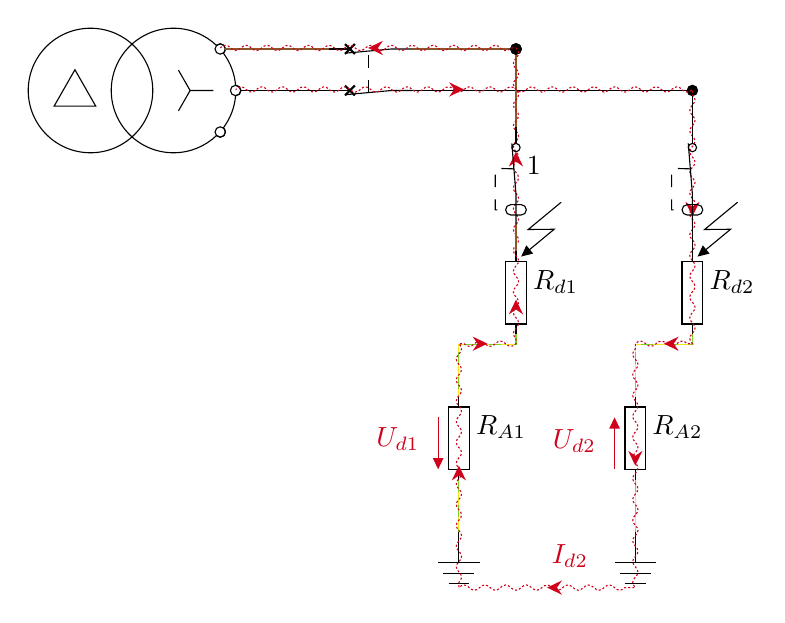
\begin{tikzpicture}[x=0.75pt,y=0.75pt,yscale=-1,xscale=1]
%uncomment if require: \path (0,314); %set diagram left start at 0, and has height of 314

%Straight Lines [id:da44771480202014247] 
\draw [color={rgb, 255:red, 0; green, 0; blue, 0 }  ,draw opacity=1 ]   (337.5,52.5) -- (337.5,35) ;
%Straight Lines [id:da5616221950341589] 
\draw    (202.5,35) -- (337.5,35) ;
%Straight Lines [id:da030139218122943512] 
\draw [color={rgb, 255:red, 139; green, 87; blue, 42 }  ,draw opacity=1 ]   (202.5,15) -- (252.5,15) ;
%Shape: Path Data [id:dp23022875443693058] 
\draw   (112.5,55) .. controls (112.5,56.38) and (111.38,57.5) .. (110,57.5) .. controls (109.29,57.5) and (108.65,57.2) .. (108.19,56.72) .. controls (102.81,61.85) and (95.52,65) .. (87.5,65) .. controls (70.93,65) and (57.5,51.57) .. (57.5,35) .. controls (57.5,18.43) and (70.93,5) .. (87.5,5) .. controls (95.52,5) and (102.81,8.15) .. (108.19,13.28) .. controls (108.65,12.8) and (109.29,12.5) .. (110,12.5) .. controls (111.38,12.5) and (112.5,13.62) .. (112.5,15) .. controls (112.5,15.82) and (112.11,16.54) .. (111.5,17) .. controls (114.8,21.39) and (116.92,26.71) .. (117.4,32.5) .. controls (117.43,32.5) and (117.47,32.5) .. (117.5,32.5) .. controls (118.88,32.5) and (120,33.62) .. (120,35) .. controls (120,36.38) and (118.88,37.5) .. (117.5,37.5) .. controls (117.47,37.5) and (117.43,37.5) .. (117.4,37.5) .. controls (116.92,43.29) and (114.8,48.61) .. (111.5,53) .. controls (112.11,53.46) and (112.5,54.18) .. (112.5,55) -- cycle ;
%Shape: Circle [id:dp1357901111827381] 
\draw   (17.5,35) .. controls (17.5,18.43) and (30.93,5) .. (47.5,5) .. controls (64.07,5) and (77.5,18.43) .. (77.5,35) .. controls (77.5,51.57) and (64.07,65) .. (47.5,65) .. controls (30.93,65) and (17.5,51.57) .. (17.5,35) -- cycle ;
%Shape: Triangle [id:dp7632621922673382] 
\draw   (40,25) -- (30,42.5) -- (50,42.5) -- cycle ;
%Shape: Star [id:dp9731649410229973] 
\draw   (106.75,35) -- (95.5,35) -- (89.88,44.81) -- (95.5,35) -- (89.88,25.19) -- (95.5,35) -- cycle ;
%Shape: Circle [id:dp31079836431690466] 
\draw   (107.5,15) .. controls (107.5,13.62) and (108.62,12.5) .. (110,12.5) .. controls (111.38,12.5) and (112.5,13.62) .. (112.5,15) .. controls (112.5,16.38) and (111.38,17.5) .. (110,17.5) .. controls (108.62,17.5) and (107.5,16.38) .. (107.5,15) -- cycle ;
%Shape: Circle [id:dp12266233820557082] 
\draw   (114.9,35) .. controls (114.9,33.62) and (116.02,32.5) .. (117.4,32.5) .. controls (118.78,32.5) and (119.9,33.62) .. (119.9,35) .. controls (119.9,36.38) and (118.78,37.5) .. (117.4,37.5) .. controls (116.02,37.5) and (114.9,36.38) .. (114.9,35) -- cycle ;
%Shape: Circle [id:dp5285901626538249] 
\draw   (107.5,55) .. controls (107.5,53.62) and (108.62,52.5) .. (110,52.5) .. controls (111.38,52.5) and (112.5,53.62) .. (112.5,55) .. controls (112.5,56.38) and (111.38,57.5) .. (110,57.5) .. controls (108.62,57.5) and (107.5,56.38) .. (107.5,55) -- cycle ;

%Straight Lines [id:da92188130951024] 
\draw [color={rgb, 255:red, 248; green, 231; blue, 28 }  ,draw opacity=1 ]   (225,222.5) -- (225,247.5) ;
%Straight Lines [id:da4292625671170487] 
\draw    (225,247.5) -- (225,262.5) ;
%Straight Lines [id:da06158937078168358] 
\draw    (215,262.5) -- (235,262.5) ;
%Straight Lines [id:da34789977188703036] 
\draw    (217.5,267.5) -- (232.5,267.5) ;
%Straight Lines [id:da1284483495628228] 
\draw    (220,272.5) -- (230,272.5) ;

%Straight Lines [id:da9082827551048067] 
\draw [color={rgb, 255:red, 126; green, 211; blue, 33 }  ,draw opacity=1 ] [dash pattern={on 4.5pt off 4.5pt}]  (225,222.5) -- (225,247.5) ;
%Straight Lines [id:da3209999402872329] 
\draw    (225,217.5) -- (225,222.5) ;
%Shape: Rectangle [id:dp2593386875607734] 
\draw   (230,187.5) -- (230,217.5) -- (220,217.5) -- (220,187.5) -- cycle ;
%Straight Lines [id:da740170600357607] 
\draw    (225,182.5) -- (225,187.5) ;

%Shape: Circle [id:dp8601483461254399] 
\draw  [fill={rgb, 255:red, 0; green, 0; blue, 0 }  ,fill opacity=1 ] (335,35) .. controls (335,33.62) and (336.12,32.5) .. (337.5,32.5) .. controls (338.88,32.5) and (340,33.62) .. (340,35) .. controls (340,36.38) and (338.88,37.5) .. (337.5,37.5) .. controls (336.12,37.5) and (335,36.38) .. (335,35) -- cycle ;
%Shape: Circle [id:dp12093020485396755] 
\draw  [fill={rgb, 255:red, 0; green, 0; blue, 0 }  ,fill opacity=1 ] (250,15) .. controls (250,13.62) and (251.12,12.5) .. (252.5,12.5) .. controls (253.88,12.5) and (255,13.62) .. (255,15) .. controls (255,16.38) and (253.88,17.5) .. (252.5,17.5) .. controls (251.12,17.5) and (250,16.38) .. (250,15) -- cycle ;
%Straight Lines [id:da2667129361258299] 
\draw [color={rgb, 255:red, 139; green, 87; blue, 42 }  ,draw opacity=1 ]   (112.5,15) -- (162.5,15) ;
%Straight Lines [id:da7247612407560878] 
\draw    (120,35) -- (162.5,35) ;
%Straight Lines [id:da9818089865990709] 
\draw    (310,217.5) -- (310,222.5) ;
%Shape: Rectangle [id:dp5739667555283554] 
\draw   (315,187.5) -- (315,217.5) -- (305,217.5) -- (305,187.5) -- cycle ;
%Straight Lines [id:da37673824938051304] 
\draw    (310,182.5) -- (310,187.5) ;

%Straight Lines [id:da9108771567706163] 
\draw [color={rgb, 255:red, 248; green, 231; blue, 28 }  ,draw opacity=1 ]   (310,222.5) -- (310,247.5) ;
%Straight Lines [id:da7506296134174059] 
\draw    (310,247.5) -- (310,262.5) ;
%Straight Lines [id:da8877376114904583] 
\draw    (300,262.5) -- (320,262.5) ;
%Straight Lines [id:da7805584248970565] 
\draw    (302.5,267.5) -- (317.5,267.5) ;
%Straight Lines [id:da4987046828919294] 
\draw    (305,272.5) -- (315,272.5) ;

%Straight Lines [id:da07069683992258613] 
\draw [color={rgb, 255:red, 126; green, 211; blue, 33 }  ,draw opacity=1 ] [dash pattern={on 4.5pt off 4.5pt}]  (310,222.5) -- (310,247.5) ;
%Shape: Boxed Line [id:dp017806634598713234] 
\draw    (274.27,88.83) -- (258.39,101.97) -- (270.89,101.86) -- (257.31,113.09) ;
\draw [shift={(255,115)}, rotate = 320.40999999999997] [fill={rgb, 255:red, 0; green, 0; blue, 0 }  ][line width=0.08]  [draw opacity=0] (5.36,-2.57) -- (0,0) -- (5.36,2.57) -- cycle    ;
%Shape: Boxed Line [id:dp8065003718686437] 
\draw    (359.27,88.83) -- (343.39,101.97) -- (355.89,101.86) -- (342.31,113.09) ;
\draw [shift={(340,115)}, rotate = 320.40999999999997] [fill={rgb, 255:red, 0; green, 0; blue, 0 }  ][line width=0.08]  [draw opacity=0] (5.36,-2.57) -- (0,0) -- (5.36,2.57) -- cycle    ;
%Straight Lines [id:da358454328833814] 
\draw    (170.5,37) -- (192.5,35) -- (202.5,35) ;
%Straight Lines [id:da868029205565597] 
\draw    (172.5,35) -- (162.5,35) ;
\draw [shift={(172.5,35)}, rotate = 225] [color={rgb, 255:red, 0; green, 0; blue, 0 }  ][line width=0.75]    (-3.35,0) -- (3.35,0)(0,3.35) -- (0,-3.35)   ;
%Straight Lines [id:da5656192330750602] 
\draw    (170.5,17) -- (192.5,15) -- (202.5,15) ;
%Straight Lines [id:da95863135682658] 
\draw  [dash pattern={on 4.5pt off 4.5pt}]  (181.5,36) -- (181.5,16) ;
%Straight Lines [id:da04894585565347964] 
\draw    (172.5,15) -- (162.5,15) ;
\draw [shift={(172.5,15)}, rotate = 225] [color={rgb, 255:red, 0; green, 0; blue, 0 }  ][line width=0.75]    (-3.35,0) -- (3.35,0)(0,3.35) -- (0,-3.35)   ;

%Straight Lines [id:da3293738134254155] 
\draw [color={rgb, 255:red, 139; green, 87; blue, 42 }  ,draw opacity=1 ]   (252.5,52.5) -- (252.5,15) ;
%Shape: Circle [id:dp8784736615935372] 
\draw  [fill={rgb, 255:red, 0; green, 0; blue, 0 }  ,fill opacity=1 ] (250,15) .. controls (250,13.62) and (251.12,12.5) .. (252.5,12.5) .. controls (253.88,12.5) and (255,13.62) .. (255,15) .. controls (255,16.38) and (253.88,17.5) .. (252.5,17.5) .. controls (251.12,17.5) and (250,16.38) .. (250,15) -- cycle ;
%Shape: Circle [id:dp11711924104585536] 
\draw  [fill={rgb, 255:red, 0; green, 0; blue, 0 }  ,fill opacity=1 ] (250,15) .. controls (250,13.62) and (251.12,12.5) .. (252.5,12.5) .. controls (253.88,12.5) and (255,13.62) .. (255,15) .. controls (255,16.38) and (253.88,17.5) .. (252.5,17.5) .. controls (251.12,17.5) and (250,16.38) .. (250,15) -- cycle ;
%Straight Lines [id:da08029921398538342] 
\draw    (252.5,147.5) -- (252.5,152.5) ;
%Shape: Rectangle [id:dp10461869500763998] 
\draw   (257.5,117.5) -- (257.5,147.5) -- (247.5,147.5) -- (247.5,117.5) -- cycle ;
%Straight Lines [id:da6711839663438437] 
\draw    (252.5,112.5) -- (252.5,117.5) ;

%Straight Lines [id:da306978016539733] 
\draw [color={rgb, 255:red, 208; green, 2; blue, 27 }  ,draw opacity=1 ]   (215,192.5) -- (215,214.5) ;
\draw [shift={(215,217.5)}, rotate = 270] [fill={rgb, 255:red, 208; green, 2; blue, 27 }  ,fill opacity=1 ][line width=0.08]  [draw opacity=0] (5.36,-2.57) -- (0,0) -- (5.36,2.57) -- cycle    ;
%Straight Lines [id:da9788903429329091] 
\draw [color={rgb, 255:red, 248; green, 231; blue, 28 }  ,draw opacity=1 ]   (252.5,152.5) -- (252.5,157.5) -- (225,157.5) -- (225,182.5) ;
%Straight Lines [id:da5746028122478745] 
\draw [color={rgb, 255:red, 126; green, 211; blue, 33 }  ,draw opacity=1 ] [dash pattern={on 4.5pt off 4.5pt}]  (252.5,152.5) -- (252.5,157.5) -- (225,157.5) -- (225,182.5) ;
%Straight Lines [id:da6637901588667133] 
\draw    (337.5,147.5) -- (337.5,152.5) ;
%Shape: Rectangle [id:dp33834418757589935] 
\draw   (342.5,117.5) -- (342.5,147.5) -- (332.5,147.5) -- (332.5,117.5) -- cycle ;
%Straight Lines [id:da4844708396236749] 
\draw    (337.5,112.5) -- (337.5,117.5) ;

%Straight Lines [id:da4767279022409927] 
\draw [color={rgb, 255:red, 208; green, 2; blue, 27 }  ,draw opacity=1 ]   (300,195.5) -- (300,217.5) ;
\draw [shift={(300,192.5)}, rotate = 90] [fill={rgb, 255:red, 208; green, 2; blue, 27 }  ,fill opacity=1 ][line width=0.08]  [draw opacity=0] (5.36,-2.57) -- (0,0) -- (5.36,2.57) -- cycle    ;
%Straight Lines [id:da015083238595793191] 
\draw [color={rgb, 255:red, 248; green, 231; blue, 28 }  ,draw opacity=1 ]   (337.5,152.5) -- (337.5,157.5) -- (310,157.5) -- (310,182.5) ;
%Straight Lines [id:da013265453939943717] 
\draw [color={rgb, 255:red, 126; green, 211; blue, 33 }  ,draw opacity=1 ] [dash pattern={on 4.5pt off 4.5pt}]  (337.5,152.5) -- (337.5,157.5) -- (310,157.5) -- (310,182.5) ;
%Straight Lines [id:da20369483289006973] 
\draw [color={rgb, 255:red, 208; green, 2; blue, 27 }  ,draw opacity=1 ] [dash pattern={on 0.75pt off 0.75pt}]  (110,14.5) .. controls (111.67,12.83) and (113.33,12.83) .. (115,14.5) .. controls (116.67,16.17) and (118.33,16.17) .. (120,14.5) .. controls (121.67,12.83) and (123.33,12.83) .. (125,14.5) .. controls (126.67,16.17) and (128.33,16.17) .. (130,14.5) .. controls (131.67,12.83) and (133.33,12.83) .. (135,14.5) .. controls (136.67,16.17) and (138.33,16.17) .. (140,14.5) .. controls (141.67,12.83) and (143.33,12.83) .. (145,14.5) .. controls (146.67,16.17) and (148.33,16.17) .. (150,14.5) .. controls (151.67,12.83) and (153.33,12.83) .. (155,14.5) .. controls (156.67,16.17) and (158.33,16.17) .. (160,14.5) .. controls (161.67,12.83) and (163.33,12.83) .. (165,14.5) .. controls (166.67,16.17) and (168.33,16.17) .. (170,14.5) .. controls (171.67,12.83) and (173.33,12.83) .. (175,14.5) .. controls (176.67,16.17) and (178.33,16.17) .. (180,14.5) .. controls (181.67,12.83) and (183.33,12.83) .. (185,14.5) .. controls (186.67,16.17) and (188.33,16.17) .. (190,14.5) .. controls (191.67,12.83) and (193.33,12.83) .. (195,14.5) .. controls (196.67,16.17) and (198.33,16.17) .. (200,14.5) .. controls (201.67,12.83) and (203.33,12.83) .. (205,14.5) .. controls (206.67,16.17) and (208.33,16.17) .. (210,14.5) .. controls (211.67,12.83) and (213.33,12.83) .. (215,14.5) .. controls (216.67,16.17) and (218.33,16.17) .. (220,14.5) .. controls (221.67,12.83) and (223.33,12.83) .. (225,14.5) .. controls (226.67,16.17) and (228.33,16.17) .. (230,14.5) .. controls (231.67,12.83) and (233.33,12.83) .. (235,14.5) .. controls (236.67,16.17) and (238.33,16.17) .. (240,14.5) .. controls (241.67,12.83) and (243.33,12.83) .. (245,14.5) .. controls (246.67,16.17) and (248.33,16.17) .. (250,14.5) -- (252.5,14.5) -- (252.5,14.5) .. controls (254.17,16.17) and (254.17,17.83) .. (252.5,19.5) .. controls (250.83,21.17) and (250.83,22.83) .. (252.5,24.5) .. controls (254.17,26.17) and (254.17,27.83) .. (252.5,29.5) .. controls (250.83,31.17) and (250.83,32.83) .. (252.5,34.5) .. controls (254.17,36.17) and (254.17,37.83) .. (252.5,39.5) .. controls (250.83,41.17) and (250.83,42.83) .. (252.5,44.5) .. controls (254.17,46.17) and (254.17,47.83) .. (252.5,49.5) .. controls (250.83,51.17) and (250.83,52.83) .. (252.5,54.5) .. controls (254.17,56.17) and (254.17,57.83) .. (252.5,59.5) .. controls (250.83,61.17) and (250.83,62.83) .. (252.5,64.5) .. controls (254.17,66.17) and (254.17,67.83) .. (252.5,69.5) .. controls (250.83,71.17) and (250.83,72.83) .. (252.5,74.5) .. controls (254.17,76.17) and (254.17,77.83) .. (252.5,79.5) .. controls (250.83,81.17) and (250.83,82.83) .. (252.5,84.5) .. controls (254.17,86.17) and (254.17,87.83) .. (252.5,89.5) .. controls (250.83,91.17) and (250.83,92.83) .. (252.5,94.5) .. controls (254.17,96.17) and (254.17,97.83) .. (252.5,99.5) .. controls (250.83,101.17) and (250.83,102.83) .. (252.5,104.5) .. controls (254.17,106.17) and (254.17,107.83) .. (252.5,109.5) .. controls (250.83,111.17) and (250.83,112.83) .. (252.5,114.5) -- (252.5,114.5) .. controls (254.17,116.17) and (254.17,117.83) .. (252.5,119.5) .. controls (250.83,121.17) and (250.83,122.83) .. (252.5,124.5) .. controls (254.17,126.17) and (254.17,127.83) .. (252.5,129.5) .. controls (250.83,131.17) and (250.83,132.83) .. (252.5,134.5) .. controls (254.17,136.17) and (254.17,137.83) .. (252.5,139.5) .. controls (250.83,141.17) and (250.83,142.83) .. (252.5,144.5) .. controls (254.17,146.17) and (254.17,147.83) .. (252.5,149.5) .. controls (250.83,151.17) and (250.83,152.83) .. (252.5,154.5) -- (252.5,157) -- (252.5,157) .. controls (250.83,158.67) and (249.17,158.67) .. (247.5,157) .. controls (245.83,155.33) and (244.17,155.33) .. (242.5,157) .. controls (240.83,158.67) and (239.17,158.67) .. (237.5,157) .. controls (235.83,155.33) and (234.17,155.33) .. (232.5,157) .. controls (230.83,158.67) and (229.17,158.67) .. (227.5,157) -- (225,157) -- (225,157) .. controls (226.67,158.67) and (226.67,160.33) .. (225,162) .. controls (223.33,163.67) and (223.33,165.33) .. (225,167) .. controls (226.67,168.67) and (226.67,170.33) .. (225,172) .. controls (223.33,173.67) and (223.33,175.33) .. (225,177) .. controls (226.67,178.67) and (226.67,180.33) .. (225,182) .. controls (223.33,183.67) and (223.33,185.33) .. (225,187) .. controls (226.67,188.67) and (226.67,190.33) .. (225,192) .. controls (223.33,193.67) and (223.33,195.33) .. (225,197) .. controls (226.67,198.67) and (226.67,200.33) .. (225,202) .. controls (223.33,203.67) and (223.33,205.33) .. (225,207) .. controls (226.67,208.67) and (226.67,210.33) .. (225,212) .. controls (223.33,213.67) and (223.33,215.33) .. (225,217) .. controls (226.67,218.67) and (226.67,220.33) .. (225,222) .. controls (223.33,223.67) and (223.33,225.33) .. (225,227) .. controls (226.67,228.67) and (226.67,230.33) .. (225,232) .. controls (223.33,233.67) and (223.33,235.33) .. (225,237) .. controls (226.67,238.67) and (226.67,240.33) .. (225,242) .. controls (223.33,243.67) and (223.33,245.33) .. (225,247) .. controls (226.67,248.67) and (226.67,250.33) .. (225,252) .. controls (223.33,253.67) and (223.33,255.33) .. (225,257) .. controls (226.67,258.67) and (226.67,260.33) .. (225,262) .. controls (223.33,263.67) and (223.33,265.33) .. (225,267) .. controls (226.67,268.67) and (226.67,270.33) .. (225,272) -- (225,274.5) -- (225,274.5) .. controls (226.67,272.83) and (228.33,272.83) .. (230,274.5) .. controls (231.67,276.17) and (233.33,276.17) .. (235,274.5) .. controls (236.67,272.83) and (238.33,272.83) .. (240,274.5) .. controls (241.67,276.17) and (243.33,276.17) .. (245,274.5) .. controls (246.67,272.83) and (248.33,272.83) .. (250,274.5) .. controls (251.67,276.17) and (253.33,276.17) .. (255,274.5) .. controls (256.67,272.83) and (258.33,272.83) .. (260,274.5) .. controls (261.67,276.17) and (263.33,276.17) .. (265,274.5) .. controls (266.67,272.83) and (268.33,272.83) .. (270,274.5) .. controls (271.67,276.17) and (273.33,276.17) .. (275,274.5) .. controls (276.67,272.83) and (278.33,272.83) .. (280,274.5) .. controls (281.67,276.17) and (283.33,276.17) .. (285,274.5) .. controls (286.67,272.83) and (288.33,272.83) .. (290,274.5) .. controls (291.67,276.17) and (293.33,276.17) .. (295,274.5) .. controls (296.67,272.83) and (298.33,272.83) .. (300,274.5) .. controls (301.67,276.17) and (303.33,276.17) .. (305,274.5) -- (310,274.5) -- (310,274.5) .. controls (308.33,272.83) and (308.33,271.17) .. (310,269.5) .. controls (311.67,267.83) and (311.67,266.17) .. (310,264.5) .. controls (308.33,262.83) and (308.33,261.17) .. (310,259.5) .. controls (311.67,257.83) and (311.67,256.17) .. (310,254.5) .. controls (308.33,252.83) and (308.33,251.17) .. (310,249.5) .. controls (311.67,247.83) and (311.67,246.17) .. (310,244.5) .. controls (308.33,242.83) and (308.33,241.17) .. (310,239.5) .. controls (311.67,237.83) and (311.67,236.17) .. (310,234.5) .. controls (308.33,232.83) and (308.33,231.17) .. (310,229.5) .. controls (311.67,227.83) and (311.67,226.17) .. (310,224.5) .. controls (308.33,222.83) and (308.33,221.17) .. (310,219.5) .. controls (311.67,217.83) and (311.67,216.17) .. (310,214.5) .. controls (308.33,212.83) and (308.33,211.17) .. (310,209.5) .. controls (311.67,207.83) and (311.67,206.17) .. (310,204.5) .. controls (308.33,202.83) and (308.33,201.17) .. (310,199.5) .. controls (311.67,197.83) and (311.67,196.17) .. (310,194.5) .. controls (308.33,192.83) and (308.33,191.17) .. (310,189.5) .. controls (311.67,187.83) and (311.67,186.17) .. (310,184.5) .. controls (308.33,182.83) and (308.33,181.17) .. (310,179.5) .. controls (311.67,177.83) and (311.67,176.17) .. (310,174.5) .. controls (308.33,172.83) and (308.33,171.17) .. (310,169.5) .. controls (311.67,167.83) and (311.67,166.17) .. (310,164.5) .. controls (308.33,162.83) and (308.33,161.17) .. (310,159.5) -- (310,157) -- (310,157) .. controls (311.67,155.33) and (313.33,155.33) .. (315,157) .. controls (316.67,158.67) and (318.33,158.67) .. (320,157) .. controls (321.67,155.33) and (323.33,155.33) .. (325,157) .. controls (326.67,158.67) and (328.33,158.67) .. (330,157) .. controls (331.67,155.33) and (333.33,155.33) .. (335,157) -- (337.5,157) -- (337.5,157) .. controls (335.83,155.33) and (335.83,153.67) .. (337.5,152) .. controls (339.17,150.33) and (339.17,148.67) .. (337.5,147) .. controls (335.83,145.33) and (335.83,143.67) .. (337.5,142) .. controls (339.17,140.33) and (339.17,138.67) .. (337.5,137) .. controls (335.83,135.33) and (335.83,133.67) .. (337.5,132) .. controls (339.17,130.33) and (339.17,128.67) .. (337.5,127) .. controls (335.83,125.33) and (335.83,123.67) .. (337.5,122) .. controls (339.17,120.33) and (339.17,118.67) .. (337.5,117) .. controls (335.83,115.33) and (335.83,113.67) .. (337.5,112) .. controls (339.17,110.33) and (339.17,108.67) .. (337.5,107) .. controls (335.83,105.33) and (335.83,103.67) .. (337.5,102) .. controls (339.17,100.33) and (339.17,98.67) .. (337.5,97) .. controls (335.83,95.33) and (335.83,93.67) .. (337.5,92) .. controls (339.17,90.33) and (339.17,88.67) .. (337.5,87) .. controls (335.83,85.33) and (335.83,83.67) .. (337.5,82) .. controls (339.17,80.33) and (339.17,78.67) .. (337.5,77) .. controls (335.83,75.33) and (335.83,73.67) .. (337.5,72) .. controls (339.17,70.33) and (339.17,68.67) .. (337.5,67) .. controls (335.83,65.33) and (335.83,63.67) .. (337.5,62) .. controls (339.17,60.33) and (339.17,58.67) .. (337.5,57) .. controls (335.83,55.33) and (335.83,53.67) .. (337.5,52) .. controls (339.17,50.33) and (339.17,48.67) .. (337.5,47) .. controls (335.83,45.33) and (335.83,43.67) .. (337.5,42) .. controls (339.17,40.33) and (339.17,38.67) .. (337.5,37) -- (337.5,34.5) -- (337.5,34.5) .. controls (335.83,36.17) and (334.17,36.17) .. (332.5,34.5) .. controls (330.83,32.83) and (329.17,32.83) .. (327.5,34.5) .. controls (325.83,36.17) and (324.17,36.17) .. (322.5,34.5) .. controls (320.83,32.83) and (319.17,32.83) .. (317.5,34.5) .. controls (315.83,36.17) and (314.17,36.17) .. (312.5,34.5) .. controls (310.83,32.83) and (309.17,32.83) .. (307.5,34.5) .. controls (305.83,36.17) and (304.17,36.17) .. (302.5,34.5) .. controls (300.83,32.83) and (299.17,32.83) .. (297.5,34.5) .. controls (295.83,36.17) and (294.17,36.17) .. (292.5,34.5) .. controls (290.83,32.83) and (289.17,32.83) .. (287.5,34.5) .. controls (285.83,36.17) and (284.17,36.17) .. (282.5,34.5) .. controls (280.83,32.83) and (279.17,32.83) .. (277.5,34.5) .. controls (275.83,36.17) and (274.17,36.17) .. (272.5,34.5) .. controls (270.83,32.83) and (269.17,32.83) .. (267.5,34.5) .. controls (265.83,36.17) and (264.17,36.17) .. (262.5,34.5) .. controls (260.83,32.83) and (259.17,32.83) .. (257.5,34.5) .. controls (255.83,36.17) and (254.17,36.17) .. (252.5,34.5) .. controls (250.83,32.83) and (249.17,32.83) .. (247.5,34.5) .. controls (245.83,36.17) and (244.17,36.17) .. (242.5,34.5) .. controls (240.83,32.83) and (239.17,32.83) .. (237.5,34.5) .. controls (235.83,36.17) and (234.17,36.17) .. (232.5,34.5) .. controls (230.83,32.83) and (229.17,32.83) .. (227.5,34.5) .. controls (225.83,36.17) and (224.17,36.17) .. (222.5,34.5) .. controls (220.83,32.83) and (219.17,32.83) .. (217.5,34.5) .. controls (215.83,36.17) and (214.17,36.17) .. (212.5,34.5) .. controls (210.83,32.83) and (209.17,32.83) .. (207.5,34.5) .. controls (205.83,36.17) and (204.17,36.17) .. (202.5,34.5) .. controls (200.83,32.83) and (199.17,32.83) .. (197.5,34.5) .. controls (195.83,36.17) and (194.17,36.17) .. (192.5,34.5) .. controls (190.83,32.83) and (189.17,32.83) .. (187.5,34.5) .. controls (185.83,36.17) and (184.17,36.17) .. (182.5,34.5) .. controls (180.83,32.83) and (179.17,32.83) .. (177.5,34.5) .. controls (175.83,36.17) and (174.17,36.17) .. (172.5,34.5) .. controls (170.83,32.83) and (169.17,32.83) .. (167.5,34.5) .. controls (165.83,36.17) and (164.17,36.17) .. (162.5,34.5) .. controls (160.83,32.83) and (159.17,32.83) .. (157.5,34.5) .. controls (155.83,36.17) and (154.17,36.17) .. (152.5,34.5) .. controls (150.83,32.83) and (149.17,32.83) .. (147.5,34.5) .. controls (145.83,36.17) and (144.17,36.17) .. (142.5,34.5) .. controls (140.83,32.83) and (139.17,32.83) .. (137.5,34.5) .. controls (135.83,36.17) and (134.17,36.17) .. (132.5,34.5) .. controls (130.83,32.83) and (129.17,32.83) .. (127.5,34.5) .. controls (125.83,36.17) and (124.17,36.17) .. (122.5,34.5) .. controls (120.83,32.83) and (119.17,32.83) .. (117.5,34.5) -- (117.4,34.5) -- (117.4,34.5) ;
\draw [shift={(181.25,14.5)}, rotate = 0] [fill={rgb, 255:red, 208; green, 2; blue, 27 }  ,fill opacity=1 ][line width=0.08]  [draw opacity=0] (7.14,-3.43) -- (0,0) -- (7.14,3.43) -- (4.74,0) -- cycle    ;
\draw [shift={(252.5,64.5)}, rotate = 90] [fill={rgb, 255:red, 208; green, 2; blue, 27 }  ,fill opacity=1 ][line width=0.08]  [draw opacity=0] (7.14,-3.43) -- (0,0) -- (7.14,3.43) -- (4.74,0) -- cycle    ;
\draw [shift={(252.5,135.75)}, rotate = 90] [fill={rgb, 255:red, 208; green, 2; blue, 27 }  ,fill opacity=1 ][line width=0.08]  [draw opacity=0] (7.14,-3.43) -- (0,0) -- (7.14,3.43) -- (4.74,0) -- cycle    ;
\draw [shift={(238.75,157)}, rotate = 180] [fill={rgb, 255:red, 208; green, 2; blue, 27 }  ,fill opacity=1 ][line width=0.08]  [draw opacity=0] (7.14,-3.43) -- (0,0) -- (7.14,3.43) -- (4.74,0) -- cycle    ;
\draw [shift={(225,215.75)}, rotate = 90] [fill={rgb, 255:red, 208; green, 2; blue, 27 }  ,fill opacity=1 ][line width=0.08]  [draw opacity=0] (7.14,-3.43) -- (0,0) -- (7.14,3.43) -- (4.74,0) -- cycle    ;
\draw [shift={(267.5,274.5)}, rotate = 0] [fill={rgb, 255:red, 208; green, 2; blue, 27 }  ,fill opacity=1 ][line width=0.08]  [draw opacity=0] (7.14,-3.43) -- (0,0) -- (7.14,3.43) -- (4.74,0) -- cycle    ;
\draw [shift={(310,215.75)}, rotate = 270] [fill={rgb, 255:red, 208; green, 2; blue, 27 }  ,fill opacity=1 ][line width=0.08]  [draw opacity=0] (7.14,-3.43) -- (0,0) -- (7.14,3.43) -- (4.74,0) -- cycle    ;
\draw [shift={(323.75,157)}, rotate = 0] [fill={rgb, 255:red, 208; green, 2; blue, 27 }  ,fill opacity=1 ][line width=0.08]  [draw opacity=0] (7.14,-3.43) -- (0,0) -- (7.14,3.43) -- (4.74,0) -- cycle    ;
\draw [shift={(337.5,95.75)}, rotate = 270] [fill={rgb, 255:red, 208; green, 2; blue, 27 }  ,fill opacity=1 ][line width=0.08]  [draw opacity=0] (7.14,-3.43) -- (0,0) -- (7.14,3.43) -- (4.74,0) -- cycle    ;
\draw [shift={(227.45,34.5)}, rotate = 180] [fill={rgb, 255:red, 208; green, 2; blue, 27 }  ,fill opacity=1 ][line width=0.08]  [draw opacity=0] (7.14,-3.43) -- (0,0) -- (7.14,3.43) -- (4.74,0) -- cycle    ;
%Shape: Circle [id:dp6688360070263407] 
\draw   (254.5,62.5) .. controls (254.5,61.4) and (253.6,60.5) .. (252.5,60.5) .. controls (251.4,60.5) and (250.5,61.4) .. (250.5,62.5) .. controls (250.5,63.6) and (251.4,64.5) .. (252.5,64.5) .. controls (253.6,64.5) and (254.5,63.6) .. (254.5,62.5) -- cycle ;
%Straight Lines [id:da023498503244457125] 
\draw    (252.5,60.5) -- (252.5,52.5) ;
%Rounded Rect [id:dp30279070557566734] 
\draw   (247.5,92.5) .. controls (247.5,91.12) and (248.62,90) .. (250,90) -- (255,90) .. controls (256.38,90) and (257.5,91.12) .. (257.5,92.5) -- (257.5,92.5) .. controls (257.5,93.88) and (256.38,95) .. (255,95) -- (250,95) .. controls (248.62,95) and (247.5,93.88) .. (247.5,92.5) -- cycle ;
%Straight Lines [id:da16468651371944532] 
\draw  [dash pattern={on 4.5pt off 4.5pt}]  (251.5,72.75) -- (242.5,72.5) -- (242.5,92.5) -- (247.5,92.5) ;
%Straight Lines [id:da8036936912023739] 
\draw    (250.5,60.5) -- (252.5,85) -- (252.5,100) ;

%Shape: Circle [id:dp7937625551850244] 
\draw   (339.5,62.5) .. controls (339.5,61.4) and (338.6,60.5) .. (337.5,60.5) .. controls (336.4,60.5) and (335.5,61.4) .. (335.5,62.5) .. controls (335.5,63.6) and (336.4,64.5) .. (337.5,64.5) .. controls (338.6,64.5) and (339.5,63.6) .. (339.5,62.5) -- cycle ;
%Straight Lines [id:da5242903170497772] 
\draw    (337.5,60.5) -- (337.5,52.5) ;
%Rounded Rect [id:dp6818768532487535] 
\draw   (332.5,92.5) .. controls (332.5,91.12) and (333.62,90) .. (335,90) -- (340,90) .. controls (341.38,90) and (342.5,91.12) .. (342.5,92.5) -- (342.5,92.5) .. controls (342.5,93.88) and (341.38,95) .. (340,95) -- (335,95) .. controls (333.62,95) and (332.5,93.88) .. (332.5,92.5) -- cycle ;
%Straight Lines [id:da0851882978686429] 
\draw  [dash pattern={on 4.5pt off 4.5pt}]  (336.5,72.75) -- (327.5,72.5) -- (327.5,92.5) -- (332.5,92.5) ;
%Straight Lines [id:da2719116658142192] 
\draw    (335.5,60.5) -- (337.5,85) -- (337.5,100) ;

%Straight Lines [id:da23106759511180686] 
\draw [color={rgb, 255:red, 139; green, 87; blue, 42 }  ,draw opacity=1 ]   (252.5,112.5) -- (252.5,100) ;
%Straight Lines [id:da04628877500711526] 
\draw [color={rgb, 255:red, 0; green, 0; blue, 0 }  ,draw opacity=1 ]   (337.5,112.5) -- (337.5,100) ;


% Text Node
\draw (232,190.5) node [anchor=north west][inner sep=0.75pt]   [align=left] {$R_{A1}$};
% Text Node
\draw (317,190.5) node [anchor=north west][inner sep=0.75pt]   [align=left] {$R_{A2}$};
% Text Node
\draw (268.5,252.5) node [anchor=north west][inner sep=0.75pt]  [color={rgb, 255:red, 208; green, 2; blue, 27 }  ,opacity=1 ] [align=left] {$I_{d2}$};
% Text Node
\draw (184,196) node [anchor=north west][inner sep=0.75pt]  [color={rgb, 255:red, 208; green, 2; blue, 27 }  ,opacity=1 ] [align=left] {$U_{d1}$};
% Text Node
\draw (259.5,120.5) node [anchor=north west][inner sep=0.75pt]   [align=left] {$R_{d1}$};
% Text Node
\draw (269,197) node [anchor=north west][inner sep=0.75pt]  [color={rgb, 255:red, 208; green, 2; blue, 27 }  ,opacity=1 ] [align=left] {$U_{d2}$};
% Text Node
\draw (344.5,120.5) node [anchor=north west][inner sep=0.75pt]   [align=left] {$R_{d2}$};
% Text Node
\draw (256.5,65.5) node [anchor=north west][inner sep=0.75pt]   [align=left] {\Circled{1}};

\end{tikzpicture}


\end{figure}

%\end{document}


L'intensité de courant $I_{d2}$ vaut alors :
\begin{formule}{Courant du deuxième défaut $I_{d2}$ en schéma Isolé-Individuel}{}
\begin{align*}
		I_{d2} &= \frac{U}{R_{d1}+R_{A1}+R_{A2}+R_{A2}} \\
\end{align*}

\begin{textvariables}
U								& tension nominale composée				& volt			& \volt					& 	Différence de potentiel entre deux conducteurs actifs (à préciser s'il s'agit du conducteur neutre)	\\
R_{d1}						& résistance											& ohm			& \ohm					& 	Résistance de défaut 	d'isolement de l'appareil 1\\
R_{A1}						& résistance											& ohm			& \ohm					& 	Résistance de la prise de terre de l'appareil 1 	\\
R_{A2}						& résistance											& ohm			& \ohm					& 	Résistance de la prise de terre de l'appareil 2 	\\
R_{d2}						& résistance											& ohm			& \ohm					& 	Résistance de défaut 	d'isolement de l'appareil 1\\
\end{textvariables}
\end{formule}

Le courant de défaut $I_{d1}$ fera alors apparaître une \emph{tension de défaut} $U_{d1}$ entre la masse métallique de l'appareil 1 et la terre. Cette tension, limitée par l'impédance de fuite, sera très largement inférieure à  $U_L$ et ne sera donc pas dangereuse. La situation sera similaire avec un schéma Impédant-Individuel $Z_N$, ou l'impédance de limitation limitera également le courant de défaut :

\begin{formule}{Tension de défaut $U_{d1}$ en schéma Isolé-Individuel}{}
\begin{align*}
		U_{d1} &= R_{A1} \times I_{d2} \\
					&<	U_L
\end{align*}

\begin{textvariables}
R_{A1}						& résistance											& ohm			& \ohm					& 	Résistance de la prise de terre de l'appareil 1 	\\
I_{d2}						& intensité												& ampère		& \ampere				& 	Courant de défaut de l'appareil 2 \\
U_{L}						& tension							& volt			& \volt										& 	Tension de sécurité du local avec :
\begin{description}[nosep, leftmargin=*]
\item[Local sec :] $U_{L}=\SI{50}{\volt}$
\item[Local humide :] $U_{L}=\SI{25}{\volt}$
\end{description} \\
\end{textvariables}
\end{formule}

Le cas est similaire à ceux rencontrés en schéma TT, on procèdera de la même manière en protégeant chaque groupe de masses par un DDR au calibre adapté \Circled{1}. Il est donc nécessaire de limiter $U_{d1}$ à la valeur suivante (voir \superref{form:resistance_prise_terre}) :

\begin{formule*}{Calibre du DDR $I_{\Delta n}$}{}
\begin{align*}
		I_{\Delta n} &< \frac{U_{L}}{R_{A1}}
\end{align*}

\begin{textvariables}
R_{A1}						& résistance											& ohm			& \ohm					& 	Résistance de la prise de terre de l'appareil 1 	\\
U_{L}						& tension							& volt			& \volt					& 	Tension de sécurité du local avec :
\begin{description}[nosep, leftmargin=*]
\item[Local sec :] $U_{L}=\SI{50}{\volt}$
\item[Local humide :] $U_{L}=\SI{25}{\volt}$
\end{description} \\
R_{A1}						& résistance											& ohm			& \ohm					& 	Résistance de la prise de terre de l'appareil 1 	\\
\end{textvariables}
\end{formule*}

L'usage de DDR implique de tenir du courant du premier défaut d'isolement $I_{d1}$ afin que la protection ne coupe pas le circuit dès le premier défaut :

\begin{table}[h]
\caption{Correspondance entre la capacité de fuite et le courant de premier défaut d'isolement}
\begin{tabular}{cc}
\toprule
\thead{Capacité de fuite (\si{\micro\farad})} 	&	\thead{Courant de premier défaut (\si{\ampere})} \\
\midrule
1		&	0,07 \\
5		& 0,36 \\
30		& 2,17 \\
\bottomrule
\end{tabular}
\end{table}
\begin{exemple}{Tension de défaut $U_{d1}$ en schéma Isolé-Individuel au deuxième défaut}{}
Si on considère que le transformateur est un transformateur $\SI{20}{\kilo\volt}/\SI{400}{\volt}$, que $R_{A1}=R_{A2}=\SI{40}{\ohm}$ et que $R_{d1} =R_{d1}= \SI{2}{\ohm}$, on peut déduire que le courant de défaut $I_{d2}$ vaut :
\begin{align*}
		I_{d2} &= \frac{U}{R_{d1}+R_{A1}+R_{A2}+R_{A2}} \\
					&=\frac{400}{2+40+40+2} \\
				&= \SI{4,76}{\ampere} \\
\end{align*}
Si une personne touche à la masse du récepteur 1, elle sera soumise à une tension de défaut $U_{d1}$ :
\begin{align*}
		U_{d1} &= R_{A1} \times I_{d2} \\
				&=40 \times 4,76 \\
				&= \SI{190,4}{\volt}
\end{align*}
La tension de défaut $U_{d1}$ est dangereuse quelle que soit la tension limite choisie :
\begin{itemize}
\item coupure la plus rapide possible\,;
\item protection des personnes.
\end{itemize}
~\\
\begin{minipage}[t]{0.5\linewidth}
Dans le cas d'un local sec :
\begin{align*}
	I_{\Delta n} 	&< \frac{U_{L}}{R_{A1}} \\
						&< \frac{50}{40} \\
						&< \SI{1,25}{\ampere}
\end{align*}
\end{minipage}
\hfill
\begin{minipage}[t]{0.5\linewidth}
Dans le cas d'un local humide :
\begin{align*}
	I_{\Delta n} 	&< \frac{U_{L}}{R_{A1}} \\
						&< \frac{25}{40} \\
						&< \SI{0,625}{\ampere}
\end{align*}
\end{minipage}
~\\
D'après le tableau situé en \superref{tab:temps_coupure_DDR}, le DDR protégeant la carcasse de l'appareil 1 doit présenter un temps de coupure de moins de \SI{200}{\milli\second} avec une tension de défaut $U_d$ de \SI{190,4}{\volt}.
\end{exemple}

\subsection{Neutre isolé et masses interconnectées et mise à la terre}

Les situations saines et au premier défaut d'isolement d'une installation en schéma IT avec les masses conductrices interconnectées et reliés en un seul point seront similaires au schéma IT avec les masses mise à la terre individuellement. Au deuxième défaut d'isolement, la situation sera différente, la prise en charge du défaut va s'apparenter à celle qu'on rencontre en schéma TN avec l'apparition d'un court-circuit.

 \begin{figure}[H]
\caption{Installation Isolé-Interconnectée}
\begin{subfigure}[t]{0.49\linewidth}
%--------------------------------------
%ELECTROTECHNIQUE - SCHEMA DE LIAISON A LA TERRE
%--------------------------------------

%utiliser les environnement \begin{comment} \end{comment} pour mettre en commentaire le préambule une fois la programmation appelée dans le document maître (!ne pas oublier de mettre en commentaire \end{document}!)

\begin{comment}

\documentclass[a4paper, 11pt, twoside, fleqn]{memoir}

\usepackage{AOCDTF}

\marqueurchapitre
\decoupagechapitre{1} %juste pour éviter les erreurs lors de la compilation des sous-programmations (passera en commentaire)

%lien d'édition des figures Tikz sur le site mathcha.io (rajouter le lien d'une modification effectuée sur la figure tikz avec le nom du modificateur car il n'y a qu'un lien par compte)

%lien mathcha Bruno Douchy : https://www.mathcha.io/editor/DXXG1FgjiNJCe0yo2ZTqzEeM8hlg57ygtvk5Mpy

%--------------------------------------
%corps du document
%--------------------------------------

\begin{document} %corps du document
	\openleft %début de chapitre à gauche

\end{comment}






% Pattern Info
 
\tikzset{
pattern size/.store in=\mcSize, 
pattern size = 5pt,
pattern thickness/.store in=\mcThickness, 
pattern thickness = 0.3pt,
pattern radius/.store in=\mcRadius, 
pattern radius = 1pt}
\makeatletter
\pgfutil@ifundefined{pgf@pattern@name@_kig45mqly}{
\pgfdeclarepatternformonly[\mcThickness,\mcSize]{_kig45mqly}
{\pgfqpoint{0pt}{0pt}}
{\pgfpoint{\mcSize+\mcThickness}{\mcSize+\mcThickness}}
{\pgfpoint{\mcSize}{\mcSize}}
{
\pgfsetcolor{\tikz@pattern@color}
\pgfsetlinewidth{\mcThickness}
\pgfpathmoveto{\pgfqpoint{0pt}{0pt}}
\pgfpathlineto{\pgfpoint{\mcSize+\mcThickness}{\mcSize+\mcThickness}}
\pgfusepath{stroke}
}}
\makeatother
\tikzset{every picture/.style={line width=0.5pt}} %set default line width to 0.75pt        

\begin{tikzpicture}[x=0.75pt,y=0.75pt,yscale=-0.6,xscale=0.6]
%uncomment if require: \path (0,293); %set diagram left start at 0, and has height of 293

%Straight Lines [id:da7855603359005625] 
\draw [color={rgb, 255:red, 74; green, 144; blue, 226 }  ,draw opacity=1 ]   (202.5,75.5) -- (462.5,75) ;
%Straight Lines [id:da3845932965061506] 
\draw [color={rgb, 255:red, 74; green, 144; blue, 226 }  ,draw opacity=1 ]   (90,75) -- (162.5,75) ;
%Straight Lines [id:da5834167633542386] 
\draw [color={rgb, 255:red, 248; green, 231; blue, 28 }  ,draw opacity=1 ]   (87.5,75) -- (27.5,75) -- (27.5,182.5) ;
%Straight Lines [id:da9429513177603445] 
\draw [color={rgb, 255:red, 248; green, 231; blue, 28 }  ,draw opacity=1 ]   (95.5,35) -- (87.5,75) -- (87.5,107.5) ;
%Straight Lines [id:da7600472701317061] 
\draw [color={rgb, 255:red, 126; green, 211; blue, 33 }  ,draw opacity=1 ] [dash pattern={on 2.25pt off 2.25pt}]  (95.5,35) -- (87.5,75) -- (87.5,107.5) ;
%Straight Lines [id:da6079599273540643] 
\draw [color={rgb, 255:red, 248; green, 231; blue, 28 }  ,draw opacity=1 ]   (240,135) -- (225,135) -- (225,182.5) ;
%Straight Lines [id:da8706050361736538] 
\draw    (202.5,35) -- (463.75,35) ;
%Straight Lines [id:da5697476802363065] 
\draw [color={rgb, 255:red, 139; green, 87; blue, 42 }  ,draw opacity=1 ]   (202.5,15) -- (462.5,15) ;
%Straight Lines [id:da9735954426571896] 
\draw [color={rgb, 255:red, 155; green, 155; blue, 155 }  ,draw opacity=1 ]   (202.5,55) -- (462.5,55) ;
%Shape: Path Data [id:dp36735613758138397] 
\draw   (112.5,55) .. controls (112.5,56.38) and (111.38,57.5) .. (110,57.5) .. controls (109.29,57.5) and (108.65,57.2) .. (108.19,56.72) .. controls (102.81,61.85) and (95.52,65) .. (87.5,65) .. controls (70.93,65) and (57.5,51.57) .. (57.5,35) .. controls (57.5,18.43) and (70.93,5) .. (87.5,5) .. controls (95.52,5) and (102.81,8.15) .. (108.19,13.28) .. controls (108.65,12.8) and (109.29,12.5) .. (110,12.5) .. controls (111.38,12.5) and (112.5,13.62) .. (112.5,15) .. controls (112.5,15.82) and (112.11,16.54) .. (111.5,17) .. controls (114.8,21.39) and (116.92,26.71) .. (117.4,32.5) .. controls (117.43,32.5) and (117.47,32.5) .. (117.5,32.5) .. controls (118.88,32.5) and (120,33.62) .. (120,35) .. controls (120,36.38) and (118.88,37.5) .. (117.5,37.5) .. controls (117.47,37.5) and (117.43,37.5) .. (117.4,37.5) .. controls (116.92,43.29) and (114.8,48.61) .. (111.5,53) .. controls (112.11,53.46) and (112.5,54.18) .. (112.5,55) -- cycle ;
%Shape: Circle [id:dp23421524241037028] 
\draw   (17.5,35) .. controls (17.5,18.43) and (30.93,5) .. (47.5,5) .. controls (64.07,5) and (77.5,18.43) .. (77.5,35) .. controls (77.5,51.57) and (64.07,65) .. (47.5,65) .. controls (30.93,65) and (17.5,51.57) .. (17.5,35) -- cycle ;
%Shape: Triangle [id:dp48236106138172463] 
\draw   (40,25) -- (30,42.5) -- (50,42.5) -- cycle ;
%Shape: Star [id:dp8682414008103251] 
\draw   (106.75,35) -- (95.5,35) -- (89.88,44.81) -- (95.5,35) -- (89.88,25.19) -- (95.5,35) -- cycle ;
%Shape: Circle [id:dp74403652528276] 
\draw   (107.5,15) .. controls (107.5,13.62) and (108.62,12.5) .. (110,12.5) .. controls (111.38,12.5) and (112.5,13.62) .. (112.5,15) .. controls (112.5,16.38) and (111.38,17.5) .. (110,17.5) .. controls (108.62,17.5) and (107.5,16.38) .. (107.5,15) -- cycle ;
%Shape: Circle [id:dp12230623178485356] 
\draw   (114.9,35) .. controls (114.9,33.62) and (116.02,32.5) .. (117.4,32.5) .. controls (118.78,32.5) and (119.9,33.62) .. (119.9,35) .. controls (119.9,36.38) and (118.78,37.5) .. (117.4,37.5) .. controls (116.02,37.5) and (114.9,36.38) .. (114.9,35) -- cycle ;
%Shape: Circle [id:dp8868519788786934] 
\draw   (107.5,55) .. controls (107.5,53.62) and (108.62,52.5) .. (110,52.5) .. controls (111.38,52.5) and (112.5,53.62) .. (112.5,55) .. controls (112.5,56.38) and (111.38,57.5) .. (110,57.5) .. controls (108.62,57.5) and (107.5,56.38) .. (107.5,55) -- cycle ;

%Straight Lines [id:da4565704928737364] 
\draw [color={rgb, 255:red, 74; green, 144; blue, 226 }  ,draw opacity=1 ]   (292.5,112.5) -- (292.5,77.5) ;
%Straight Lines [id:da08957212555201388] 
\draw [color={rgb, 255:red, 139; green, 87; blue, 42 }  ,draw opacity=1 ]   (252.5,112.5) -- (252.5,17.5) ;
%Straight Lines [id:da7418535885736515] 
\draw [color={rgb, 255:red, 139; green, 87; blue, 42 }  ,draw opacity=1 ]   (252.5,130) -- (252.5,117.5) ;
%Straight Lines [id:da8720965180296373] 
\draw [color={rgb, 255:red, 74; green, 144; blue, 226 }  ,draw opacity=1 ]   (292.5,130.5) -- (292.5,117.5) ;
%Straight Lines [id:da938936503356733] 
\draw    (17.5,232.5) -- (460,232.5) ;
%Shape: Rectangle [id:dp7311273665746781] 
\draw  [draw opacity=0][pattern=_kig45mqly,pattern size=6pt,pattern thickness=0.75pt,pattern radius=0pt, pattern color={rgb, 255:red, 0; green, 0; blue, 0}][line width=0.75]  (17.5,232.5) -- (460,232.5) -- (460,247.5) -- (17.5,247.5) -- cycle ;
%Straight Lines [id:da8141513336558377] 
\draw [color={rgb, 255:red, 126; green, 211; blue, 33 }  ,draw opacity=1 ] [dash pattern={on 2.25pt off 2.25pt}]  (240,135) -- (225,135) -- (225,182.5) ;
%Straight Lines [id:da29843762221307424] 
\draw [color={rgb, 255:red, 248; green, 231; blue, 28 }  ,draw opacity=1 ]   (225,222.5) -- (225,247.5) ;
%Straight Lines [id:da11084730612327653] 
\draw    (225,247.5) -- (225,262.5) ;
%Straight Lines [id:da28813972378566177] 
\draw    (215,262.5) -- (235,262.5) ;
%Straight Lines [id:da12034369105457465] 
\draw    (217.5,267.5) -- (232.5,267.5) ;
%Straight Lines [id:da6195695090232725] 
\draw    (220,272.5) -- (230,272.5) ;

%Straight Lines [id:da7010427793052417] 
\draw [color={rgb, 255:red, 126; green, 211; blue, 33 }  ,draw opacity=1 ] [dash pattern={on 2.25pt off 2.25pt}]  (225,222.5) -- (225,247.5) ;
%Straight Lines [id:da6639632595865842] 
\draw    (287.5,130) -- (292.5,130) ;
%Shape: Rectangle [id:dp48750397418832736] 
\draw   (257.5,125) -- (287.5,125) -- (287.5,135) -- (257.5,135) -- cycle ;
%Straight Lines [id:da3091869002192609] 
\draw    (252.5,130) -- (257.5,130) ;

%Straight Lines [id:da46843421066318236] 
\draw    (225,217.5) -- (225,222.5) ;
%Shape: Rectangle [id:dp8288861680700458] 
\draw   (230,187.5) -- (230,217.5) -- (220,217.5) -- (220,187.5) -- cycle ;
%Straight Lines [id:da39538233114745247] 
\draw    (225,182.5) -- (225,187.5) ;

%Straight Lines [id:da03908999537683522] 
\draw [color={rgb, 255:red, 74; green, 144; blue, 226 }  ,draw opacity=1 ]   (377.5,112.5) -- (377.5,77.5) ;
%Straight Lines [id:da014322617412467653] 
\draw [color={rgb, 255:red, 0; green, 0; blue, 0 }  ,draw opacity=1 ]   (337.5,112.5) -- (337.5,35) ;
%Straight Lines [id:da7075832342481658] 
\draw [color={rgb, 255:red, 139; green, 87; blue, 42 }  ,draw opacity=1 ]   (337.5,130) -- (337.5,117.5) ;
%Straight Lines [id:da37678293812005714] 
\draw [color={rgb, 255:red, 74; green, 144; blue, 226 }  ,draw opacity=1 ]   (377.5,130.5) -- (377.5,117.5) ;
%Straight Lines [id:da9817945211819089] 
\draw    (372.5,130) -- (377.5,130) ;
%Shape: Rectangle [id:dp3965217784422401] 
\draw   (342.5,125) -- (372.5,125) -- (372.5,135) -- (342.5,135) -- cycle ;
%Straight Lines [id:da03329133725543032] 
\draw    (337.5,130) -- (342.5,130) ;

%Straight Lines [id:da8796176191529531] 
\draw [color={rgb, 255:red, 74; green, 144; blue, 226 }  ,draw opacity=1 ]   (462.5,112.5) -- (462.5,77.5) ;
%Straight Lines [id:da6222130388950533] 
\draw [color={rgb, 255:red, 155; green, 155; blue, 155 }  ,draw opacity=1 ]   (422.5,112.5) -- (422.5,55) ;
%Straight Lines [id:da1963014933165811] 
\draw [color={rgb, 255:red, 139; green, 87; blue, 42 }  ,draw opacity=1 ]   (422.5,130) -- (422.5,117.5) ;
%Straight Lines [id:da25889379629104303] 
\draw [color={rgb, 255:red, 74; green, 144; blue, 226 }  ,draw opacity=1 ]   (462.5,130.5) -- (462.5,117.5) ;
%Straight Lines [id:da3869416860630762] 
\draw    (457.5,130) -- (462.5,130) ;
%Shape: Rectangle [id:dp6819736010368719] 
\draw   (427.5,125) -- (457.5,125) -- (457.5,135) -- (427.5,135) -- cycle ;
%Straight Lines [id:da34290626385752987] 
\draw    (422.5,130) -- (427.5,130) ;

%Shape: Circle [id:dp7660888532599164] 
\draw  [fill={rgb, 255:red, 0; green, 0; blue, 0 }  ,fill opacity=1 ] (375,75) .. controls (375,73.62) and (376.12,72.5) .. (377.5,72.5) .. controls (378.88,72.5) and (380,73.62) .. (380,75) .. controls (380,76.38) and (378.88,77.5) .. (377.5,77.5) .. controls (376.12,77.5) and (375,76.38) .. (375,75) -- cycle ;
%Shape: Circle [id:dp6916920109792153] 
\draw  [fill={rgb, 255:red, 0; green, 0; blue, 0 }  ,fill opacity=1 ] (460,75) .. controls (460,73.62) and (461.12,72.5) .. (462.5,72.5) .. controls (463.88,72.5) and (465,73.62) .. (465,75) .. controls (465,76.38) and (463.88,77.5) .. (462.5,77.5) .. controls (461.12,77.5) and (460,76.38) .. (460,75) -- cycle ;
%Shape: Circle [id:dp27655045875256845] 
\draw  [fill={rgb, 255:red, 0; green, 0; blue, 0 }  ,fill opacity=1 ] (335,35) .. controls (335,33.62) and (336.12,32.5) .. (337.5,32.5) .. controls (338.88,32.5) and (340,33.62) .. (340,35) .. controls (340,36.38) and (338.88,37.5) .. (337.5,37.5) .. controls (336.12,37.5) and (335,36.38) .. (335,35) -- cycle ;
%Shape: Circle [id:dp8031492541807427] 
\draw  [fill={rgb, 255:red, 0; green, 0; blue, 0 }  ,fill opacity=1 ] (420,55) .. controls (420,53.62) and (421.12,52.5) .. (422.5,52.5) .. controls (423.88,52.5) and (425,53.62) .. (425,55) .. controls (425,56.38) and (423.88,57.5) .. (422.5,57.5) .. controls (421.12,57.5) and (420,56.38) .. (420,55) -- cycle ;
%Shape: Circle [id:dp9192263751877222] 
\draw  [fill={rgb, 255:red, 0; green, 0; blue, 0 }  ,fill opacity=1 ] (290,75) .. controls (290,73.62) and (291.12,72.5) .. (292.5,72.5) .. controls (293.88,72.5) and (295,73.62) .. (295,75) .. controls (295,76.38) and (293.88,77.5) .. (292.5,77.5) .. controls (291.12,77.5) and (290,76.38) .. (290,75) -- cycle ;
%Shape: Circle [id:dp3725249444527118] 
\draw  [fill={rgb, 255:red, 0; green, 0; blue, 0 }  ,fill opacity=1 ] (250,15) .. controls (250,13.62) and (251.12,12.5) .. (252.5,12.5) .. controls (253.88,12.5) and (255,13.62) .. (255,15) .. controls (255,16.38) and (253.88,17.5) .. (252.5,17.5) .. controls (251.12,17.5) and (250,16.38) .. (250,15) -- cycle ;
%Shape: Rectangle [id:dp06629411116627981] 
\draw  [dash pattern={on 2.25pt off 2.25pt on 1pt off 2.25pt}] (242.5,115) -- (302.5,115) -- (302.5,145) -- (242.5,145) -- cycle ;
%Shape: Circle [id:dp3317282661895262] 
\draw  [fill={rgb, 255:red, 255; green, 255; blue, 255 }  ,fill opacity=1 ] (240,135) .. controls (240,133.62) and (241.12,132.5) .. (242.5,132.5) .. controls (243.88,132.5) and (245,133.62) .. (245,135) .. controls (245,136.38) and (243.88,137.5) .. (242.5,137.5) .. controls (241.12,137.5) and (240,136.38) .. (240,135) -- cycle ;
%Shape: Circle [id:dp705146955440835] 
\draw  [fill={rgb, 255:red, 255; green, 255; blue, 255 }  ,fill opacity=1 ] (250,115) .. controls (250,113.62) and (251.12,112.5) .. (252.5,112.5) .. controls (253.88,112.5) and (255,113.62) .. (255,115) .. controls (255,116.38) and (253.88,117.5) .. (252.5,117.5) .. controls (251.12,117.5) and (250,116.38) .. (250,115) -- cycle ;
%Shape: Circle [id:dp8927328941538174] 
\draw  [fill={rgb, 255:red, 255; green, 255; blue, 255 }  ,fill opacity=1 ] (290,115) .. controls (290,113.62) and (291.12,112.5) .. (292.5,112.5) .. controls (293.88,112.5) and (295,113.62) .. (295,115) .. controls (295,116.38) and (293.88,117.5) .. (292.5,117.5) .. controls (291.12,117.5) and (290,116.38) .. (290,115) -- cycle ;
%Shape: Rectangle [id:dp5496339182307807] 
\draw  [dash pattern={on 2.25pt off 2.25pt on 1pt off 2.25pt}] (327.5,115) -- (387.5,115) -- (387.5,145) -- (327.5,145) -- cycle ;
%Shape: Circle [id:dp08833497953402314] 
\draw  [fill={rgb, 255:red, 255; green, 255; blue, 255 }  ,fill opacity=1 ] (335,115) .. controls (335,113.62) and (336.12,112.5) .. (337.5,112.5) .. controls (338.88,112.5) and (340,113.62) .. (340,115) .. controls (340,116.38) and (338.88,117.5) .. (337.5,117.5) .. controls (336.12,117.5) and (335,116.38) .. (335,115) -- cycle ;
%Shape: Circle [id:dp022577282390605857] 
\draw  [fill={rgb, 255:red, 255; green, 255; blue, 255 }  ,fill opacity=1 ] (375,115) .. controls (375,113.62) and (376.12,112.5) .. (377.5,112.5) .. controls (378.88,112.5) and (380,113.62) .. (380,115) .. controls (380,116.38) and (378.88,117.5) .. (377.5,117.5) .. controls (376.12,117.5) and (375,116.38) .. (375,115) -- cycle ;
%Shape: Rectangle [id:dp30094494963346674] 
\draw  [dash pattern={on 2.25pt off 2.25pt on 1pt off 2.25pt}] (412.5,115) -- (472.5,115) -- (472.5,145) -- (412.5,145) -- cycle ;
%Shape: Circle [id:dp28947508340592676] 
\draw  [fill={rgb, 255:red, 255; green, 255; blue, 255 }  ,fill opacity=1 ] (420,115) .. controls (420,113.62) and (421.12,112.5) .. (422.5,112.5) .. controls (423.88,112.5) and (425,113.62) .. (425,115) .. controls (425,116.38) and (423.88,117.5) .. (422.5,117.5) .. controls (421.12,117.5) and (420,116.38) .. (420,115) -- cycle ;
%Shape: Circle [id:dp2039724957780732] 
\draw  [fill={rgb, 255:red, 255; green, 255; blue, 255 }  ,fill opacity=1 ] (460,115) .. controls (460,113.62) and (461.12,112.5) .. (462.5,112.5) .. controls (463.88,112.5) and (465,113.62) .. (465,115) .. controls (465,116.38) and (463.88,117.5) .. (462.5,117.5) .. controls (461.12,117.5) and (460,116.38) .. (460,115) -- cycle ;
%Straight Lines [id:da9086113972049343] 
\draw [color={rgb, 255:red, 139; green, 87; blue, 42 }  ,draw opacity=1 ]   (112.5,15) -- (162.5,15) ;
%Straight Lines [id:da39378818016703376] 
\draw [color={rgb, 255:red, 155; green, 155; blue, 155 }  ,draw opacity=1 ]   (112.5,55) -- (162.5,55) ;
%Straight Lines [id:da7098443885614435] 
\draw    (120,35) -- (162.5,35) ;
%Straight Lines [id:da7807923609638333] 
\draw    (87.5,217.5) -- (87.5,222.5) ;
%Shape: Rectangle [id:dp7756651140200441] 
\draw   (92.5,187.5) -- (92.5,217.5) -- (82.5,217.5) -- (82.5,187.5) -- cycle ;
%Straight Lines [id:da04032572174714] 
\draw    (87.5,182.5) -- (87.5,187.5) ;

%Straight Lines [id:da7401415732232357] 
\draw [color={rgb, 255:red, 248; green, 231; blue, 28 }  ,draw opacity=1 ]   (87.5,222.5) -- (87.5,247.5) ;
%Straight Lines [id:da8867829423247331] 
\draw    (87.5,247.5) -- (87.5,262.5) ;
%Straight Lines [id:da6182832251033938] 
\draw    (77.5,262.5) -- (97.5,262.5) ;
%Straight Lines [id:da9945605231682282] 
\draw    (80,267.5) -- (95,267.5) ;
%Straight Lines [id:da7672039428774292] 
\draw    (82.5,272.5) -- (92.5,272.5) ;

%Straight Lines [id:da6311647435025226] 
\draw [color={rgb, 255:red, 126; green, 211; blue, 33 }  ,draw opacity=1 ] [dash pattern={on 2.25pt off 2.25pt}]  (87.5,222.5) -- (87.5,247.5) ;
%Straight Lines [id:da9935280273884104] 
\draw [color={rgb, 255:red, 126; green, 211; blue, 33 }  ,draw opacity=1 ] [dash pattern={on 2.25pt off 2.25pt}]  (87.5,75) -- (27.5,75) -- (27.5,182.5) ;
%Straight Lines [id:da14093319956254402] 
\draw    (27.5,217.5) -- (27.5,222.5) ;
%Shape: Rectangle [id:dp8874460509477418] 
\draw   (32.5,187.5) -- (32.5,217.5) -- (22.5,217.5) -- (22.5,187.5) -- cycle ;
%Straight Lines [id:da8069357458595097] 
\draw    (27.5,182.5) -- (27.5,187.5) ;

%Straight Lines [id:da1556831771412326] 
\draw [color={rgb, 255:red, 248; green, 231; blue, 28 }  ,draw opacity=1 ]   (27.5,222.5) -- (27.5,247.5) ;
%Straight Lines [id:da18177923377500727] 
\draw [color={rgb, 255:red, 126; green, 211; blue, 33 }  ,draw opacity=1 ] [dash pattern={on 2.25pt off 2.25pt}]  (27.5,222.5) -- (27.5,247.5) ;
%Straight Lines [id:da6998009649261362] 
\draw    (27.5,247.5) -- (27.5,262.5) ;
%Straight Lines [id:da5527024824171923] 
\draw    (17.5,262.5) -- (37.5,262.5) ;
%Straight Lines [id:da879174168174364] 
\draw    (20,267.5) -- (35,267.5) ;
%Straight Lines [id:da871400503059965] 
\draw    (22.5,272.5) -- (32.5,272.5) ;

%Straight Lines [id:da10216267044530791] 
\draw    (87.5,107.5) -- (87.5,132) ;
\draw [shift={(87.5,135)}, rotate = 270] [fill={rgb, 255:red, 0; green, 0; blue, 0 }  ][line width=0.08]  [draw opacity=0] (5.36,-2.57) -- (0,0) -- (5.36,2.57) -- cycle    ;
%Straight Lines [id:da4334196362201017] 
\draw    (87.5,167.5) -- (87.5,143) ;
\draw [shift={(87.5,140)}, rotate = 450] [fill={rgb, 255:red, 0; green, 0; blue, 0 }  ][line width=0.08]  [draw opacity=0] (5.36,-2.57) -- (0,0) -- (5.36,2.57) -- cycle    ;

%Straight Lines [id:da48697601510764355] 
\draw [color={rgb, 255:red, 248; green, 231; blue, 28 }  ,draw opacity=1 ]   (87.5,167.5) -- (87.5,182.5) ;
%Straight Lines [id:da7671847283137146] 
\draw [color={rgb, 255:red, 126; green, 211; blue, 33 }  ,draw opacity=1 ] [dash pattern={on 2.25pt off 2.25pt}]  (87.5,167.5) -- (87.5,182.5) ;
%Straight Lines [id:da1974083843246306] 
\draw [color={rgb, 255:red, 248; green, 231; blue, 28 }  ,draw opacity=1 ]   (325,135) -- (310,135) -- (310,155) -- (225,155) ;
%Straight Lines [id:da5466139977766219] 
\draw [color={rgb, 255:red, 126; green, 211; blue, 33 }  ,draw opacity=1 ] [dash pattern={on 2.25pt off 2.25pt}]  (325,135) -- (310,135) -- (310,155) -- (225,155) ;
%Straight Lines [id:da9329542182445705] 
\draw [color={rgb, 255:red, 248; green, 231; blue, 28 }  ,draw opacity=1 ]   (410,135) -- (395,135) -- (395,170) -- (225,170) ;
%Straight Lines [id:da1632976089388658] 
\draw [color={rgb, 255:red, 126; green, 211; blue, 33 }  ,draw opacity=1 ] [dash pattern={on 2.25pt off 2.25pt}]  (410,135) -- (395,135) -- (395,170) -- (225,170) ;
%Shape: Circle [id:dp07701655400781071] 
\draw  [fill={rgb, 255:red, 255; green, 255; blue, 255 }  ,fill opacity=1 ] (325,135) .. controls (325,133.62) and (326.12,132.5) .. (327.5,132.5) .. controls (328.88,132.5) and (330,133.62) .. (330,135) .. controls (330,136.38) and (328.88,137.5) .. (327.5,137.5) .. controls (326.12,137.5) and (325,136.38) .. (325,135) -- cycle ;
%Shape: Circle [id:dp40696952093539485] 
\draw  [fill={rgb, 255:red, 255; green, 255; blue, 255 }  ,fill opacity=1 ] (410,135) .. controls (410,133.62) and (411.12,132.5) .. (412.5,132.5) .. controls (413.88,132.5) and (415,133.62) .. (415,135) .. controls (415,136.38) and (413.88,137.5) .. (412.5,137.5) .. controls (411.12,137.5) and (410,136.38) .. (410,135) -- cycle ;
%Shape: Circle [id:dp25319941734318174] 
\draw  [fill={rgb, 255:red, 0; green, 0; blue, 0 }  ,fill opacity=1 ] (222.5,155) .. controls (222.5,153.62) and (223.62,152.5) .. (225,152.5) .. controls (226.38,152.5) and (227.5,153.62) .. (227.5,155) .. controls (227.5,156.38) and (226.38,157.5) .. (225,157.5) .. controls (223.62,157.5) and (222.5,156.38) .. (222.5,155) -- cycle ;
%Shape: Circle [id:dp2607282769032745] 
\draw  [fill={rgb, 255:red, 0; green, 0; blue, 0 }  ,fill opacity=1 ] (222.5,170) .. controls (222.5,168.62) and (223.62,167.5) .. (225,167.5) .. controls (226.38,167.5) and (227.5,168.62) .. (227.5,170) .. controls (227.5,171.38) and (226.38,172.5) .. (225,172.5) .. controls (223.62,172.5) and (222.5,171.38) .. (222.5,170) -- cycle ;
%Shape: Circle [id:dp3376103119871633] 
\draw  [fill={rgb, 255:red, 0; green, 0; blue, 0 }  ,fill opacity=1 ] (85,75) .. controls (85,73.62) and (86.12,72.5) .. (87.5,72.5) .. controls (88.88,72.5) and (90,73.62) .. (90,75) .. controls (90,76.38) and (88.88,77.5) .. (87.5,77.5) .. controls (86.12,77.5) and (85,76.38) .. (85,75) -- cycle ;
%Straight Lines [id:da22044660580035758] 
\draw [color={rgb, 255:red, 208; green, 2; blue, 27 }  ,draw opacity=1 ] [dash pattern={on 0.75pt off 0.75pt}]  (110,15) .. controls (111.67,13.33) and (113.33,13.33) .. (115,15) .. controls (116.67,16.67) and (118.33,16.67) .. (120,15) .. controls (121.67,13.33) and (123.33,13.33) .. (125,15) .. controls (126.67,16.67) and (128.33,16.67) .. (130,15) .. controls (131.67,13.33) and (133.33,13.33) .. (135,15) .. controls (136.67,16.67) and (138.33,16.67) .. (140,15) .. controls (141.67,13.33) and (143.33,13.33) .. (145,15) .. controls (146.67,16.67) and (148.33,16.67) .. (150,15) .. controls (151.67,13.33) and (153.33,13.33) .. (155,15) .. controls (156.67,16.67) and (158.33,16.67) .. (160,15) .. controls (161.67,13.33) and (163.33,13.33) .. (165,15) .. controls (166.67,16.67) and (168.33,16.67) .. (170,15) .. controls (171.67,13.33) and (173.33,13.33) .. (175,15) .. controls (176.67,16.67) and (178.33,16.67) .. (180,15) .. controls (181.67,13.33) and (183.33,13.33) .. (185,15) .. controls (186.67,16.67) and (188.33,16.67) .. (190,15) .. controls (191.67,13.33) and (193.33,13.33) .. (195,15) .. controls (196.67,16.67) and (198.33,16.67) .. (200,15) .. controls (201.67,13.33) and (203.33,13.33) .. (205,15) .. controls (206.67,16.67) and (208.33,16.67) .. (210,15) .. controls (211.67,13.33) and (213.33,13.33) .. (215,15) .. controls (216.67,16.67) and (218.33,16.67) .. (220,15) .. controls (221.67,13.33) and (223.33,13.33) .. (225,15) .. controls (226.67,16.67) and (228.33,16.67) .. (230,15) .. controls (231.67,13.33) and (233.33,13.33) .. (235,15) .. controls (236.67,16.67) and (238.33,16.67) .. (240,15) .. controls (241.67,13.33) and (243.33,13.33) .. (245,15) .. controls (246.67,16.67) and (248.33,16.67) .. (250,15) -- (252.5,15) -- (252.5,15) .. controls (254.17,16.67) and (254.17,18.33) .. (252.5,20) .. controls (250.83,21.67) and (250.83,23.33) .. (252.5,25) .. controls (254.17,26.67) and (254.17,28.33) .. (252.5,30) .. controls (250.83,31.67) and (250.83,33.33) .. (252.5,35) .. controls (254.17,36.67) and (254.17,38.33) .. (252.5,40) .. controls (250.83,41.67) and (250.83,43.33) .. (252.5,45) .. controls (254.17,46.67) and (254.17,48.33) .. (252.5,50) .. controls (250.83,51.67) and (250.83,53.33) .. (252.5,55) .. controls (254.17,56.67) and (254.17,58.33) .. (252.5,60) .. controls (250.83,61.67) and (250.83,63.33) .. (252.5,65) .. controls (254.17,66.67) and (254.17,68.33) .. (252.5,70) .. controls (250.83,71.67) and (250.83,73.33) .. (252.5,75) .. controls (254.17,76.67) and (254.17,78.33) .. (252.5,80) .. controls (250.83,81.67) and (250.83,83.33) .. (252.5,85) .. controls (254.17,86.67) and (254.17,88.33) .. (252.5,90) .. controls (250.83,91.67) and (250.83,93.33) .. (252.5,95) .. controls (254.17,96.67) and (254.17,98.33) .. (252.5,100) .. controls (250.83,101.67) and (250.83,103.33) .. (252.5,105) .. controls (254.17,106.67) and (254.17,108.33) .. (252.5,110) .. controls (250.83,111.67) and (250.83,113.33) .. (252.5,115) -- (252.5,115) .. controls (250.83,116.67) and (249.17,116.67) .. (247.5,115) .. controls (245.83,113.33) and (244.17,113.33) .. (242.5,115) -- (242.5,115) .. controls (244.17,116.67) and (244.17,118.33) .. (242.5,120) .. controls (240.83,121.67) and (240.83,123.33) .. (242.5,125) .. controls (244.17,126.67) and (244.17,128.33) .. (242.5,130) .. controls (240.83,131.67) and (240.83,133.33) .. (242.5,135) -- (242.5,135) .. controls (240.83,136.67) and (239.17,136.67) .. (237.5,135) .. controls (235.83,133.33) and (234.17,133.33) .. (232.5,135) .. controls (230.83,136.67) and (229.17,136.67) .. (227.5,135) -- (225,135) -- (225,135) .. controls (226.67,136.67) and (226.67,138.33) .. (225,140) .. controls (223.33,141.67) and (223.33,143.33) .. (225,145) .. controls (226.67,146.67) and (226.67,148.33) .. (225,150) .. controls (223.33,151.67) and (223.33,153.33) .. (225,155) .. controls (226.67,156.67) and (226.67,158.33) .. (225,160) .. controls (223.33,161.67) and (223.33,163.33) .. (225,165) .. controls (226.67,166.67) and (226.67,168.33) .. (225,170) .. controls (223.33,171.67) and (223.33,173.33) .. (225,175) .. controls (226.67,176.67) and (226.67,178.33) .. (225,180) .. controls (223.33,181.67) and (223.33,183.33) .. (225,185) .. controls (226.67,186.67) and (226.67,188.33) .. (225,190) .. controls (223.33,191.67) and (223.33,193.33) .. (225,195) .. controls (226.67,196.67) and (226.67,198.33) .. (225,200) .. controls (223.33,201.67) and (223.33,203.33) .. (225,205) .. controls (226.67,206.67) and (226.67,208.33) .. (225,210) .. controls (223.33,211.67) and (223.33,213.33) .. (225,215) .. controls (226.67,216.67) and (226.67,218.33) .. (225,220) .. controls (223.33,221.67) and (223.33,223.33) .. (225,225) .. controls (226.67,226.67) and (226.67,228.33) .. (225,230) .. controls (223.33,231.67) and (223.33,233.33) .. (225,235) .. controls (226.67,236.67) and (226.67,238.33) .. (225,240) .. controls (223.33,241.67) and (223.33,243.33) .. (225,245) .. controls (226.67,246.67) and (226.67,248.33) .. (225,250) .. controls (223.33,251.67) and (223.33,253.33) .. (225,255) .. controls (226.67,256.67) and (226.67,258.33) .. (225,260) .. controls (223.33,261.67) and (223.33,263.33) .. (225,265) .. controls (226.67,266.67) and (226.67,268.33) .. (225,270) .. controls (223.33,271.67) and (223.33,273.33) .. (225,275) -- (225,275) .. controls (223.33,276.67) and (221.67,276.67) .. (220,275) .. controls (218.33,273.33) and (216.67,273.33) .. (215,275) .. controls (213.33,276.67) and (211.67,276.67) .. (210,275) .. controls (208.33,273.33) and (206.67,273.33) .. (205,275) .. controls (203.33,276.67) and (201.67,276.67) .. (200,275) .. controls (198.33,273.33) and (196.67,273.33) .. (195,275) .. controls (193.33,276.67) and (191.67,276.67) .. (190,275) .. controls (188.33,273.33) and (186.67,273.33) .. (185,275) .. controls (183.33,276.67) and (181.67,276.67) .. (180,275) .. controls (178.33,273.33) and (176.67,273.33) .. (175,275) .. controls (173.33,276.67) and (171.67,276.67) .. (170,275) .. controls (168.33,273.33) and (166.67,273.33) .. (165,275) .. controls (163.33,276.67) and (161.67,276.67) .. (160,275) .. controls (158.33,273.33) and (156.67,273.33) .. (155,275) .. controls (153.33,276.67) and (151.67,276.67) .. (150,275) .. controls (148.33,273.33) and (146.67,273.33) .. (145,275) .. controls (143.33,276.67) and (141.67,276.67) .. (140,275) .. controls (138.33,273.33) and (136.67,273.33) .. (135,275) .. controls (133.33,276.67) and (131.67,276.67) .. (130,275) .. controls (128.33,273.33) and (126.67,273.33) .. (125,275) .. controls (123.33,276.67) and (121.67,276.67) .. (120,275) .. controls (118.33,273.33) and (116.67,273.33) .. (115,275) .. controls (113.33,276.67) and (111.67,276.67) .. (110,275) .. controls (108.33,273.33) and (106.67,273.33) .. (105,275) .. controls (103.33,276.67) and (101.67,276.67) .. (100,275) .. controls (98.33,273.33) and (96.67,273.33) .. (95,275) .. controls (93.33,276.67) and (91.67,276.67) .. (90,275) .. controls (88.33,273.33) and (86.67,273.33) .. (85,275) .. controls (83.33,276.67) and (81.67,276.67) .. (80,275) .. controls (78.33,273.33) and (76.67,273.33) .. (75,275) .. controls (73.33,276.67) and (71.67,276.67) .. (70,275) .. controls (68.33,273.33) and (66.67,273.33) .. (65,275) .. controls (63.33,276.67) and (61.67,276.67) .. (60,275) .. controls (58.33,273.33) and (56.67,273.33) .. (55,275) .. controls (53.33,276.67) and (51.67,276.67) .. (50,275) .. controls (48.33,273.33) and (46.67,273.33) .. (45,275) .. controls (43.33,276.67) and (41.67,276.67) .. (40,275) .. controls (38.33,273.33) and (36.67,273.33) .. (35,275) .. controls (33.33,276.67) and (31.67,276.67) .. (30,275) -- (27.5,275) -- (27.5,275) .. controls (25.83,273.33) and (25.83,271.67) .. (27.5,270) .. controls (29.17,268.33) and (29.17,266.67) .. (27.5,265) .. controls (25.83,263.33) and (25.83,261.67) .. (27.5,260) .. controls (29.17,258.33) and (29.17,256.67) .. (27.5,255) .. controls (25.83,253.33) and (25.83,251.67) .. (27.5,250) .. controls (29.17,248.33) and (29.17,246.67) .. (27.5,245) .. controls (25.83,243.33) and (25.83,241.67) .. (27.5,240) .. controls (29.17,238.33) and (29.17,236.67) .. (27.5,235) .. controls (25.83,233.33) and (25.83,231.67) .. (27.5,230) .. controls (29.17,228.33) and (29.17,226.67) .. (27.5,225) .. controls (25.83,223.33) and (25.83,221.67) .. (27.5,220) .. controls (29.17,218.33) and (29.17,216.67) .. (27.5,215) .. controls (25.83,213.33) and (25.83,211.67) .. (27.5,210) .. controls (29.17,208.33) and (29.17,206.67) .. (27.5,205) .. controls (25.83,203.33) and (25.83,201.67) .. (27.5,200) .. controls (29.17,198.33) and (29.17,196.67) .. (27.5,195) .. controls (25.83,193.33) and (25.83,191.67) .. (27.5,190) .. controls (29.17,188.33) and (29.17,186.67) .. (27.5,185) .. controls (25.83,183.33) and (25.83,181.67) .. (27.5,180) .. controls (29.17,178.33) and (29.17,176.67) .. (27.5,175) .. controls (25.83,173.33) and (25.83,171.67) .. (27.5,170) .. controls (29.17,168.33) and (29.17,166.67) .. (27.5,165) .. controls (25.83,163.33) and (25.83,161.67) .. (27.5,160) .. controls (29.17,158.33) and (29.17,156.67) .. (27.5,155) .. controls (25.83,153.33) and (25.83,151.67) .. (27.5,150) .. controls (29.17,148.33) and (29.17,146.67) .. (27.5,145) .. controls (25.83,143.33) and (25.83,141.67) .. (27.5,140) .. controls (29.17,138.33) and (29.17,136.67) .. (27.5,135) .. controls (25.83,133.33) and (25.83,131.67) .. (27.5,130) .. controls (29.17,128.33) and (29.17,126.67) .. (27.5,125) .. controls (25.83,123.33) and (25.83,121.67) .. (27.5,120) .. controls (29.17,118.33) and (29.17,116.67) .. (27.5,115) .. controls (25.83,113.33) and (25.83,111.67) .. (27.5,110) .. controls (29.17,108.33) and (29.17,106.67) .. (27.5,105) .. controls (25.83,103.33) and (25.83,101.67) .. (27.5,100) .. controls (29.17,98.33) and (29.17,96.67) .. (27.5,95) .. controls (25.83,93.33) and (25.83,91.67) .. (27.5,90) .. controls (29.17,88.33) and (29.17,86.67) .. (27.5,85) .. controls (25.83,83.33) and (25.83,81.67) .. (27.5,80) .. controls (29.17,78.33) and (29.17,76.67) .. (27.5,75) -- (27.5,75) .. controls (29.17,73.33) and (30.83,73.33) .. (32.5,75) .. controls (34.17,76.67) and (35.83,76.67) .. (37.5,75) .. controls (39.17,73.33) and (40.83,73.33) .. (42.5,75) .. controls (44.17,76.67) and (45.83,76.67) .. (47.5,75) .. controls (49.17,73.33) and (50.83,73.33) .. (52.5,75) .. controls (54.17,76.67) and (55.83,76.67) .. (57.5,75) .. controls (59.17,73.33) and (60.83,73.33) .. (62.5,75) .. controls (64.17,76.67) and (65.83,76.67) .. (67.5,75) .. controls (69.17,73.33) and (70.83,73.33) .. (72.5,75) .. controls (74.17,76.67) and (75.83,76.67) .. (77.5,75) .. controls (79.17,73.33) and (80.83,73.33) .. (82.5,75) .. controls (84.17,76.67) and (85.83,76.67) .. (87.5,75) -- (87.5,75) .. controls (86.19,73.04) and (86.52,71.41) .. (88.48,70.1) .. controls (90.44,68.79) and (90.77,67.15) .. (89.46,65.19) .. controls (88.15,63.23) and (88.48,61.6) .. (90.44,60.29) .. controls (92.4,58.98) and (92.73,57.35) .. (91.42,55.39) .. controls (90.11,53.43) and (90.44,51.8) .. (92.4,50.49) .. controls (94.36,49.18) and (94.69,47.54) .. (93.38,45.58) .. controls (92.07,43.62) and (92.4,41.99) .. (94.36,40.68) .. controls (96.32,39.37) and (96.65,37.74) .. (95.34,35.78) -- (95.5,35) -- (95.5,35) ;
\draw [shift={(181.25,15)}, rotate = 180] [fill={rgb, 255:red, 208; green, 2; blue, 27 }  ,fill opacity=1 ][line width=0.08]  [draw opacity=0] (5.36,-2.57) -- (0,0) -- (5.36,2.57) -- cycle    ;
\draw [shift={(252.5,65)}, rotate = 270] [fill={rgb, 255:red, 208; green, 2; blue, 27 }  ,fill opacity=1 ][line width=0.08]  [draw opacity=0] (5.36,-2.57) -- (0,0) -- (5.36,2.57) -- cycle    ;
\draw [shift={(247.5,115)}, rotate = 360] [fill={rgb, 255:red, 208; green, 2; blue, 27 }  ,fill opacity=1 ][line width=0.08]  [draw opacity=0] (5.36,-2.57) -- (0,0) -- (5.36,2.57) -- cycle    ;
\draw [shift={(242.5,125)}, rotate = 270] [fill={rgb, 255:red, 208; green, 2; blue, 27 }  ,fill opacity=1 ][line width=0.08]  [draw opacity=0] (5.36,-2.57) -- (0,0) -- (5.36,2.57) -- cycle    ;
\draw [shift={(233.75,135)}, rotate = 360] [fill={rgb, 255:red, 208; green, 2; blue, 27 }  ,fill opacity=1 ][line width=0.08]  [draw opacity=0] (5.36,-2.57) -- (0,0) -- (5.36,2.57) -- cycle    ;
\draw [shift={(225,205)}, rotate = 270] [fill={rgb, 255:red, 208; green, 2; blue, 27 }  ,fill opacity=1 ][line width=0.08]  [draw opacity=0] (5.36,-2.57) -- (0,0) -- (5.36,2.57) -- cycle    ;
\draw [shift={(126.25,275)}, rotate = 360] [fill={rgb, 255:red, 208; green, 2; blue, 27 }  ,fill opacity=1 ][line width=0.08]  [draw opacity=0] (5.36,-2.57) -- (0,0) -- (5.36,2.57) -- cycle    ;
\draw [shift={(27.5,175)}, rotate = 450] [fill={rgb, 255:red, 208; green, 2; blue, 27 }  ,fill opacity=1 ][line width=0.08]  [draw opacity=0] (5.36,-2.57) -- (0,0) -- (5.36,2.57) -- cycle    ;
\draw [shift={(57.5,75)}, rotate = 180] [fill={rgb, 255:red, 208; green, 2; blue, 27 }  ,fill opacity=1 ][line width=0.08]  [draw opacity=0] (5.36,-2.57) -- (0,0) -- (5.36,2.57) -- cycle    ;
\draw [shift={(91.5,55)}, rotate = 461.31] [fill={rgb, 255:red, 208; green, 2; blue, 27 }  ,fill opacity=1 ][line width=0.08]  [draw opacity=0] (5.36,-2.57) -- (0,0) -- (5.36,2.57) -- cycle    ;
%Straight Lines [id:da555189741163598] 
\draw    (170.5,77.5) -- (192.5,75.5) -- (202.5,75.5) ;
%Straight Lines [id:da5511404727485181] 
\draw    (172.5,75) -- (162.5,75) ;
\draw [shift={(172.5,75)}, rotate = 225] [color={rgb, 255:red, 0; green, 0; blue, 0 }  ][line width=0.75]    (-3.35,0) -- (3.35,0)(0,3.35) -- (0,-3.35)   ;
%Straight Lines [id:da8826295723719044] 
\draw    (170.5,57) -- (192.5,55) -- (202.5,55) ;
%Straight Lines [id:da7071802738172622] 
\draw  [dash pattern={on 2.25pt off 2.25pt}]  (181.5,76.5) -- (181.5,16) ;
%Straight Lines [id:da28669457007849575] 
\draw    (170.5,37) -- (192.5,35) -- (202.5,35) ;
%Straight Lines [id:da7277928540627319] 
\draw    (172.5,55) -- (162.5,55) ;
\draw [shift={(172.5,55)}, rotate = 225] [color={rgb, 255:red, 0; green, 0; blue, 0 }  ][line width=0.75]    (-3.35,0) -- (3.35,0)(0,3.35) -- (0,-3.35)   ;
%Straight Lines [id:da5845851558162967] 
\draw    (172.5,35) -- (162.5,35) ;
\draw [shift={(172.5,35)}, rotate = 225] [color={rgb, 255:red, 0; green, 0; blue, 0 }  ][line width=0.75]    (-3.35,0) -- (3.35,0)(0,3.35) -- (0,-3.35)   ;
%Straight Lines [id:da9317779613389213] 
\draw    (170.5,17) -- (192.5,15) -- (202.5,15) ;
%Straight Lines [id:da16075358030401588] 
\draw    (172.5,15) -- (162.5,15) ;
\draw [shift={(172.5,15)}, rotate = 225] [color={rgb, 255:red, 0; green, 0; blue, 0 }  ][line width=0.75]    (-3.35,0) -- (3.35,0)(0,3.35) -- (0,-3.35)   ;


% Text Node
\draw (293.5,94.5) node [anchor=north west][inner sep=0.75pt]   [align=left] {1};
% Text Node
\draw (378.5,94.5) node [anchor=north west][inner sep=0.75pt]   [align=left] {2};
% Text Node
\draw (463.5,94.5) node [anchor=north west][inner sep=0.75pt]   [align=left] {3};
% Text Node
\draw (464,7) node [anchor=north west][inner sep=0.75pt]   [align=left] {L1};
% Text Node
\draw (464,27) node [anchor=north west][inner sep=0.75pt]   [align=left] {L2};
% Text Node
\draw (465,47) node [anchor=north west][inner sep=0.75pt]   [align=left] {L3};
% Text Node
\draw (466.5,67) node [anchor=north west][inner sep=0.75pt]   [align=left] {N};
% Text Node
\draw (94.5,190.5) node [anchor=north west][inner sep=0.75pt]   [align=left] {$R_B$};
% Text Node
\draw (232,190.5) node [anchor=north west][inner sep=0.75pt]   [align=left] {$R_A$};
% Text Node
\draw (34.5,190.5) node [anchor=north west][inner sep=0.75pt]   [align=left] {$Z_{res}$};
% Text Node
\draw (136,250) node [anchor=north west][inner sep=0.75pt]  [color={rgb, 255:red, 208; green, 2; blue, 27 }  ,opacity=1 ] [align=left] {$I_{d1}$};


\end{tikzpicture}

%\end{document}

\subcaption{avec un premier défaut d'isolement}
\end{subfigure}
\begin{subfigure}[t]{0.49\linewidth}
%--------------------------------------
%ELECTROTECHNIQUE - SCHEMA DE LIAISON A LA TERRE
%--------------------------------------

%utiliser les environnement \begin{comment} \end{comment} pour mettre en commentaire le préambule une fois la programmation appelée dans le document maître (!ne pas oublier de mettre en commentaire \end{document}!)

\begin{comment}

\documentclass[a4paper, 11pt, twoside, fleqn]{memoir}

\usepackage{AOCDTF}

\marqueurchapitre
\decoupagechapitre{1} %juste pour éviter les erreurs lors de la compilation des sous-programmations (passera en commentaire)

%lien d'édition des figures Tikz sur le site mathcha.io (rajouter le lien d'une modification effectuée sur la figure tikz avec le nom du modificateur car il n'y a qu'un lien par compte)

%lien mathcha Bruno Douchy : https://www.mathcha.io/editor/d99MohP8twWsGvG0q7h9Vnz2eTLLO69jc6nZvpP

%--------------------------------------
%corps du document
%--------------------------------------

\begin{document} %corps du document
	\openleft %début de chapitre à gauche

\end{comment}






% Pattern Info
 
\tikzset{
pattern size/.store in=\mcSize, 
pattern size = 5pt,
pattern thickness/.store in=\mcThickness, 
pattern thickness = 0.3pt,
pattern radius/.store in=\mcRadius, 
pattern radius = 1pt}
\makeatletter
\pgfutil@ifundefined{pgf@pattern@name@_3d3x60i8q}{
\pgfdeclarepatternformonly[\mcThickness,\mcSize]{_3d3x60i8q}
{\pgfqpoint{0pt}{0pt}}
{\pgfpoint{\mcSize+\mcThickness}{\mcSize+\mcThickness}}
{\pgfpoint{\mcSize}{\mcSize}}
{
\pgfsetcolor{\tikz@pattern@color}
\pgfsetlinewidth{\mcThickness}
\pgfpathmoveto{\pgfqpoint{0pt}{0pt}}
\pgfpathlineto{\pgfpoint{\mcSize+\mcThickness}{\mcSize+\mcThickness}}
\pgfusepath{stroke}
}}
\makeatother
\tikzset{every picture/.style={line width=0.5pt}} %set default line width to 0.75pt        

\begin{tikzpicture}[x=0.75pt,y=0.75pt,yscale=-0.6,xscale=0.6]
%uncomment if require: \path (0,293); %set diagram left start at 0, and has height of 293

%Straight Lines [id:da4316112300950584] 
\draw [color={rgb, 255:red, 74; green, 144; blue, 226 }  ,draw opacity=1 ]   (202.5,75.5) -- (462.5,75) ;
%Straight Lines [id:da592395340901707] 
\draw [color={rgb, 255:red, 74; green, 144; blue, 226 }  ,draw opacity=1 ]   (90,75) -- (162.5,75) ;
%Straight Lines [id:da7613925009339874] 
\draw [color={rgb, 255:red, 248; green, 231; blue, 28 }  ,draw opacity=1 ]   (87.5,75) -- (27.5,75) -- (27.5,182.5) ;
%Straight Lines [id:da20815919893717771] 
\draw [color={rgb, 255:red, 248; green, 231; blue, 28 }  ,draw opacity=1 ]   (95.5,35) -- (87.5,75) -- (87.5,107.5) ;
%Straight Lines [id:da2803448246584893] 
\draw [color={rgb, 255:red, 126; green, 211; blue, 33 }  ,draw opacity=1 ] [dash pattern={on 2.25pt off 2.25pt}]  (95.5,35) -- (87.5,75) -- (87.5,107.5) ;
%Straight Lines [id:da6655486156631886] 
\draw [color={rgb, 255:red, 248; green, 231; blue, 28 }  ,draw opacity=1 ]   (240,135) -- (225,135) -- (225,182.5) ;
%Straight Lines [id:da6484833403668159] 
\draw    (202.5,35) -- (462.5,35) ;
%Straight Lines [id:da33957414836189403] 
\draw [color={rgb, 255:red, 139; green, 87; blue, 42 }  ,draw opacity=1 ]   (202.5,15) -- (462.5,15) ;
%Straight Lines [id:da16085307772389335] 
\draw [color={rgb, 255:red, 155; green, 155; blue, 155 }  ,draw opacity=1 ]   (202.5,55) -- (462.5,55) ;
%Shape: Path Data [id:dp10249500032929337] 
\draw   (112.5,55) .. controls (112.5,56.38) and (111.38,57.5) .. (110,57.5) .. controls (109.29,57.5) and (108.65,57.2) .. (108.19,56.72) .. controls (102.81,61.85) and (95.52,65) .. (87.5,65) .. controls (70.93,65) and (57.5,51.57) .. (57.5,35) .. controls (57.5,18.43) and (70.93,5) .. (87.5,5) .. controls (95.52,5) and (102.81,8.15) .. (108.19,13.28) .. controls (108.65,12.8) and (109.29,12.5) .. (110,12.5) .. controls (111.38,12.5) and (112.5,13.62) .. (112.5,15) .. controls (112.5,15.82) and (112.11,16.54) .. (111.5,17) .. controls (114.8,21.39) and (116.92,26.71) .. (117.4,32.5) .. controls (117.43,32.5) and (117.47,32.5) .. (117.5,32.5) .. controls (118.88,32.5) and (120,33.62) .. (120,35) .. controls (120,36.38) and (118.88,37.5) .. (117.5,37.5) .. controls (117.47,37.5) and (117.43,37.5) .. (117.4,37.5) .. controls (116.92,43.29) and (114.8,48.61) .. (111.5,53) .. controls (112.11,53.46) and (112.5,54.18) .. (112.5,55) -- cycle ;
%Shape: Circle [id:dp3581782398495783] 
\draw   (17.5,35) .. controls (17.5,18.43) and (30.93,5) .. (47.5,5) .. controls (64.07,5) and (77.5,18.43) .. (77.5,35) .. controls (77.5,51.57) and (64.07,65) .. (47.5,65) .. controls (30.93,65) and (17.5,51.57) .. (17.5,35) -- cycle ;
%Shape: Triangle [id:dp3866997568728687] 
\draw   (40,25) -- (30,42.5) -- (50,42.5) -- cycle ;
%Shape: Star [id:dp01594631881962638] 
\draw   (106.75,35) -- (95.5,35) -- (89.88,44.81) -- (95.5,35) -- (89.88,25.19) -- (95.5,35) -- cycle ;
%Shape: Circle [id:dp5232205694306733] 
\draw   (107.5,15) .. controls (107.5,13.62) and (108.62,12.5) .. (110,12.5) .. controls (111.38,12.5) and (112.5,13.62) .. (112.5,15) .. controls (112.5,16.38) and (111.38,17.5) .. (110,17.5) .. controls (108.62,17.5) and (107.5,16.38) .. (107.5,15) -- cycle ;
%Shape: Circle [id:dp9342995473747882] 
\draw   (114.9,35) .. controls (114.9,33.62) and (116.02,32.5) .. (117.4,32.5) .. controls (118.78,32.5) and (119.9,33.62) .. (119.9,35) .. controls (119.9,36.38) and (118.78,37.5) .. (117.4,37.5) .. controls (116.02,37.5) and (114.9,36.38) .. (114.9,35) -- cycle ;
%Shape: Circle [id:dp6020396186633284] 
\draw   (107.5,55) .. controls (107.5,53.62) and (108.62,52.5) .. (110,52.5) .. controls (111.38,52.5) and (112.5,53.62) .. (112.5,55) .. controls (112.5,56.38) and (111.38,57.5) .. (110,57.5) .. controls (108.62,57.5) and (107.5,56.38) .. (107.5,55) -- cycle ;

%Straight Lines [id:da7356919321884693] 
\draw [color={rgb, 255:red, 74; green, 144; blue, 226 }  ,draw opacity=1 ]   (292.5,112.5) -- (292.5,77.5) ;
%Straight Lines [id:da7707322948577742] 
\draw [color={rgb, 255:red, 139; green, 87; blue, 42 }  ,draw opacity=1 ]   (252.5,112.5) -- (252.5,17.5) ;
%Straight Lines [id:da3393094282652437] 
\draw [color={rgb, 255:red, 139; green, 87; blue, 42 }  ,draw opacity=1 ]   (252.5,130) -- (252.5,117.5) ;
%Straight Lines [id:da32471814491871454] 
\draw [color={rgb, 255:red, 74; green, 144; blue, 226 }  ,draw opacity=1 ]   (292.5,130.5) -- (292.5,117.5) ;
%Straight Lines [id:da2804881303921053] 
\draw    (17.5,232.5) -- (460,232.5) ;
%Shape: Rectangle [id:dp9697762095732098] 
\draw  [draw opacity=0][pattern=_3d3x60i8q,pattern size=6pt,pattern thickness=0.75pt,pattern radius=0pt, pattern color={rgb, 255:red, 0; green, 0; blue, 0}][line width=0.75]  (17.5,232.5) -- (460,232.5) -- (460,247.5) -- (17.5,247.5) -- cycle ;
%Straight Lines [id:da4471247596078385] 
\draw [color={rgb, 255:red, 126; green, 211; blue, 33 }  ,draw opacity=1 ] [dash pattern={on 2.25pt off 2.25pt}]  (240,135) -- (225,135) -- (225,182.5) ;
%Straight Lines [id:da8216134048282633] 
\draw [color={rgb, 255:red, 248; green, 231; blue, 28 }  ,draw opacity=1 ]   (225,222.5) -- (225,247.5) ;
%Straight Lines [id:da0021397444679995825] 
\draw    (225,247.5) -- (225,262.5) ;
%Straight Lines [id:da7553632333793844] 
\draw    (215,262.5) -- (235,262.5) ;
%Straight Lines [id:da3271693405574221] 
\draw    (217.5,267.5) -- (232.5,267.5) ;
%Straight Lines [id:da03574333606289193] 
\draw    (220,272.5) -- (230,272.5) ;

%Straight Lines [id:da9287696118141909] 
\draw [color={rgb, 255:red, 126; green, 211; blue, 33 }  ,draw opacity=1 ] [dash pattern={on 2.25pt off 2.25pt}]  (225,222.5) -- (225,247.5) ;
%Straight Lines [id:da4934539373464967] 
\draw    (287.5,130) -- (292.5,130) ;
%Shape: Rectangle [id:dp9292588656763955] 
\draw   (257.5,125) -- (287.5,125) -- (287.5,135) -- (257.5,135) -- cycle ;
%Straight Lines [id:da7473211177947267] 
\draw    (252.5,130) -- (257.5,130) ;

%Straight Lines [id:da486338882685015] 
\draw    (225,217.5) -- (225,222.5) ;
%Shape: Rectangle [id:dp6082154928452261] 
\draw   (230,187.5) -- (230,217.5) -- (220,217.5) -- (220,187.5) -- cycle ;
%Straight Lines [id:da02741001735829296] 
\draw    (225,182.5) -- (225,187.5) ;

%Straight Lines [id:da8337137721631095] 
\draw [color={rgb, 255:red, 74; green, 144; blue, 226 }  ,draw opacity=1 ]   (377.5,112.5) -- (377.5,77.5) ;
%Straight Lines [id:da1665166934917245] 
\draw [color={rgb, 255:red, 0; green, 0; blue, 0 }  ,draw opacity=1 ]   (337.5,112.5) -- (337.5,35) ;
%Straight Lines [id:da49866332950963677] 
\draw [color={rgb, 255:red, 139; green, 87; blue, 42 }  ,draw opacity=1 ]   (337.5,130) -- (337.5,117.5) ;
%Straight Lines [id:da06212849397856712] 
\draw [color={rgb, 255:red, 74; green, 144; blue, 226 }  ,draw opacity=1 ]   (377.5,130.5) -- (377.5,117.5) ;
%Straight Lines [id:da10583602514925727] 
\draw    (372.5,130) -- (377.5,130) ;
%Shape: Rectangle [id:dp9826719102179569] 
\draw   (342.5,125) -- (372.5,125) -- (372.5,135) -- (342.5,135) -- cycle ;
%Straight Lines [id:da9469006809288678] 
\draw    (337.5,130) -- (342.5,130) ;

%Straight Lines [id:da24022521518811535] 
\draw [color={rgb, 255:red, 74; green, 144; blue, 226 }  ,draw opacity=1 ]   (462.5,112.5) -- (462.5,77.5) ;
%Straight Lines [id:da422569463919366] 
\draw [color={rgb, 255:red, 155; green, 155; blue, 155 }  ,draw opacity=1 ]   (422.5,112.5) -- (422.5,55) ;
%Straight Lines [id:da4089426711784393] 
\draw [color={rgb, 255:red, 139; green, 87; blue, 42 }  ,draw opacity=1 ]   (422.5,130) -- (422.5,117.5) ;
%Straight Lines [id:da3209682580746803] 
\draw [color={rgb, 255:red, 74; green, 144; blue, 226 }  ,draw opacity=1 ]   (462.5,130.5) -- (462.5,117.5) ;
%Straight Lines [id:da8297703646860478] 
\draw    (457.5,130) -- (462.5,130) ;
%Shape: Rectangle [id:dp06561013483408318] 
\draw   (427.5,125) -- (457.5,125) -- (457.5,135) -- (427.5,135) -- cycle ;
%Straight Lines [id:da5296249512546637] 
\draw    (422.5,130) -- (427.5,130) ;

%Shape: Circle [id:dp14705499744377126] 
\draw  [fill={rgb, 255:red, 0; green, 0; blue, 0 }  ,fill opacity=1 ] (375,75) .. controls (375,73.62) and (376.12,72.5) .. (377.5,72.5) .. controls (378.88,72.5) and (380,73.62) .. (380,75) .. controls (380,76.38) and (378.88,77.5) .. (377.5,77.5) .. controls (376.12,77.5) and (375,76.38) .. (375,75) -- cycle ;
%Shape: Circle [id:dp487736850492963] 
\draw  [fill={rgb, 255:red, 0; green, 0; blue, 0 }  ,fill opacity=1 ] (460,75) .. controls (460,73.62) and (461.12,72.5) .. (462.5,72.5) .. controls (463.88,72.5) and (465,73.62) .. (465,75) .. controls (465,76.38) and (463.88,77.5) .. (462.5,77.5) .. controls (461.12,77.5) and (460,76.38) .. (460,75) -- cycle ;
%Shape: Circle [id:dp09964051897099524] 
\draw  [fill={rgb, 255:red, 0; green, 0; blue, 0 }  ,fill opacity=1 ] (335,35) .. controls (335,33.62) and (336.12,32.5) .. (337.5,32.5) .. controls (338.88,32.5) and (340,33.62) .. (340,35) .. controls (340,36.38) and (338.88,37.5) .. (337.5,37.5) .. controls (336.12,37.5) and (335,36.38) .. (335,35) -- cycle ;
%Shape: Circle [id:dp3177503541910154] 
\draw  [fill={rgb, 255:red, 0; green, 0; blue, 0 }  ,fill opacity=1 ] (420,55) .. controls (420,53.62) and (421.12,52.5) .. (422.5,52.5) .. controls (423.88,52.5) and (425,53.62) .. (425,55) .. controls (425,56.38) and (423.88,57.5) .. (422.5,57.5) .. controls (421.12,57.5) and (420,56.38) .. (420,55) -- cycle ;
%Shape: Circle [id:dp49609371082954723] 
\draw  [fill={rgb, 255:red, 0; green, 0; blue, 0 }  ,fill opacity=1 ] (290,75) .. controls (290,73.62) and (291.12,72.5) .. (292.5,72.5) .. controls (293.88,72.5) and (295,73.62) .. (295,75) .. controls (295,76.38) and (293.88,77.5) .. (292.5,77.5) .. controls (291.12,77.5) and (290,76.38) .. (290,75) -- cycle ;
%Shape: Circle [id:dp3317781328805872] 
\draw  [fill={rgb, 255:red, 0; green, 0; blue, 0 }  ,fill opacity=1 ] (250,15) .. controls (250,13.62) and (251.12,12.5) .. (252.5,12.5) .. controls (253.88,12.5) and (255,13.62) .. (255,15) .. controls (255,16.38) and (253.88,17.5) .. (252.5,17.5) .. controls (251.12,17.5) and (250,16.38) .. (250,15) -- cycle ;
%Shape: Rectangle [id:dp8458026238078075] 
\draw  [dash pattern={on 2.25pt off 2.25pt on 1pt off 2.25pt}] (242.5,115) -- (302.5,115) -- (302.5,145) -- (242.5,145) -- cycle ;
%Shape: Circle [id:dp4839887842470103] 
\draw  [fill={rgb, 255:red, 255; green, 255; blue, 255 }  ,fill opacity=1 ] (240,135) .. controls (240,133.62) and (241.12,132.5) .. (242.5,132.5) .. controls (243.88,132.5) and (245,133.62) .. (245,135) .. controls (245,136.38) and (243.88,137.5) .. (242.5,137.5) .. controls (241.12,137.5) and (240,136.38) .. (240,135) -- cycle ;
%Shape: Circle [id:dp23200535427044433] 
\draw  [fill={rgb, 255:red, 255; green, 255; blue, 255 }  ,fill opacity=1 ] (250,115) .. controls (250,113.62) and (251.12,112.5) .. (252.5,112.5) .. controls (253.88,112.5) and (255,113.62) .. (255,115) .. controls (255,116.38) and (253.88,117.5) .. (252.5,117.5) .. controls (251.12,117.5) and (250,116.38) .. (250,115) -- cycle ;
%Shape: Circle [id:dp43816804006827426] 
\draw  [fill={rgb, 255:red, 255; green, 255; blue, 255 }  ,fill opacity=1 ] (290,115) .. controls (290,113.62) and (291.12,112.5) .. (292.5,112.5) .. controls (293.88,112.5) and (295,113.62) .. (295,115) .. controls (295,116.38) and (293.88,117.5) .. (292.5,117.5) .. controls (291.12,117.5) and (290,116.38) .. (290,115) -- cycle ;
%Shape: Rectangle [id:dp17294192480398818] 
\draw  [dash pattern={on 2.25pt off 2.25pt on 1pt off 2.25pt}] (327.5,115) -- (387.5,115) -- (387.5,145) -- (327.5,145) -- cycle ;
%Shape: Circle [id:dp5641937149360905] 
\draw  [fill={rgb, 255:red, 255; green, 255; blue, 255 }  ,fill opacity=1 ] (335,115) .. controls (335,113.62) and (336.12,112.5) .. (337.5,112.5) .. controls (338.88,112.5) and (340,113.62) .. (340,115) .. controls (340,116.38) and (338.88,117.5) .. (337.5,117.5) .. controls (336.12,117.5) and (335,116.38) .. (335,115) -- cycle ;
%Shape: Circle [id:dp7032786941320301] 
\draw  [fill={rgb, 255:red, 255; green, 255; blue, 255 }  ,fill opacity=1 ] (375,115) .. controls (375,113.62) and (376.12,112.5) .. (377.5,112.5) .. controls (378.88,112.5) and (380,113.62) .. (380,115) .. controls (380,116.38) and (378.88,117.5) .. (377.5,117.5) .. controls (376.12,117.5) and (375,116.38) .. (375,115) -- cycle ;
%Shape: Rectangle [id:dp5708004680643411] 
\draw  [dash pattern={on 2.25pt off 2.25pt on 1pt off 2.25pt}] (412.5,115) -- (472.5,115) -- (472.5,145) -- (412.5,145) -- cycle ;
%Shape: Circle [id:dp6908523735716476] 
\draw  [fill={rgb, 255:red, 255; green, 255; blue, 255 }  ,fill opacity=1 ] (420,115) .. controls (420,113.62) and (421.12,112.5) .. (422.5,112.5) .. controls (423.88,112.5) and (425,113.62) .. (425,115) .. controls (425,116.38) and (423.88,117.5) .. (422.5,117.5) .. controls (421.12,117.5) and (420,116.38) .. (420,115) -- cycle ;
%Shape: Circle [id:dp7956677228195491] 
\draw  [fill={rgb, 255:red, 255; green, 255; blue, 255 }  ,fill opacity=1 ] (460,115) .. controls (460,113.62) and (461.12,112.5) .. (462.5,112.5) .. controls (463.88,112.5) and (465,113.62) .. (465,115) .. controls (465,116.38) and (463.88,117.5) .. (462.5,117.5) .. controls (461.12,117.5) and (460,116.38) .. (460,115) -- cycle ;
%Straight Lines [id:da8597697949860761] 
\draw [color={rgb, 255:red, 139; green, 87; blue, 42 }  ,draw opacity=1 ]   (112.5,15) -- (162.5,15) ;
%Straight Lines [id:da23077448284325242] 
\draw [color={rgb, 255:red, 155; green, 155; blue, 155 }  ,draw opacity=1 ]   (112.5,55) -- (162.5,55) ;
%Straight Lines [id:da14455238991946961] 
\draw    (120,35) -- (162.5,35) ;
%Straight Lines [id:da47305420272514154] 
\draw    (87.5,217.5) -- (87.5,222.5) ;
%Shape: Rectangle [id:dp40600391165753114] 
\draw   (92.5,187.5) -- (92.5,217.5) -- (82.5,217.5) -- (82.5,187.5) -- cycle ;
%Straight Lines [id:da7674520793059064] 
\draw    (87.5,182.5) -- (87.5,187.5) ;

%Straight Lines [id:da13592089644066174] 
\draw [color={rgb, 255:red, 248; green, 231; blue, 28 }  ,draw opacity=1 ]   (87.5,222.5) -- (87.5,247.5) ;
%Straight Lines [id:da6995969912761094] 
\draw    (87.5,247.5) -- (87.5,262.5) ;
%Straight Lines [id:da8974480356939065] 
\draw    (77.5,262.5) -- (97.5,262.5) ;
%Straight Lines [id:da14743994933249238] 
\draw    (80,267.5) -- (95,267.5) ;
%Straight Lines [id:da7671801759067333] 
\draw    (82.5,272.5) -- (92.5,272.5) ;

%Straight Lines [id:da8007274329269651] 
\draw [color={rgb, 255:red, 126; green, 211; blue, 33 }  ,draw opacity=1 ] [dash pattern={on 2.25pt off 2.25pt}]  (87.5,222.5) -- (87.5,247.5) ;
%Straight Lines [id:da2715308600728248] 
\draw [color={rgb, 255:red, 126; green, 211; blue, 33 }  ,draw opacity=1 ] [dash pattern={on 2.25pt off 2.25pt}]  (87.5,75) -- (27.5,75) -- (27.5,182.5) ;
%Straight Lines [id:da03783213481594272] 
\draw    (27.5,217.5) -- (27.5,222.5) ;
%Shape: Rectangle [id:dp15674809213871121] 
\draw   (32.5,187.5) -- (32.5,217.5) -- (22.5,217.5) -- (22.5,187.5) -- cycle ;
%Straight Lines [id:da6989887953310521] 
\draw    (27.5,182.5) -- (27.5,187.5) ;

%Straight Lines [id:da059986961359160706] 
\draw [color={rgb, 255:red, 248; green, 231; blue, 28 }  ,draw opacity=1 ]   (27.5,222.5) -- (27.5,247.5) ;
%Straight Lines [id:da22515617446341774] 
\draw [color={rgb, 255:red, 126; green, 211; blue, 33 }  ,draw opacity=1 ] [dash pattern={on 2.25pt off 2.25pt}]  (27.5,222.5) -- (27.5,247.5) ;
%Straight Lines [id:da21110515454430878] 
\draw    (27.5,247.5) -- (27.5,262.5) ;
%Straight Lines [id:da11657345325909974] 
\draw    (17.5,262.5) -- (37.5,262.5) ;
%Straight Lines [id:da9145508474375904] 
\draw    (20,267.5) -- (35,267.5) ;
%Straight Lines [id:da8054890152252306] 
\draw    (22.5,272.5) -- (32.5,272.5) ;

%Straight Lines [id:da5490636326446755] 
\draw    (87.5,107.5) -- (87.5,132) ;
\draw [shift={(87.5,135)}, rotate = 270] [fill={rgb, 255:red, 0; green, 0; blue, 0 }  ][line width=0.08]  [draw opacity=0] (5.36,-2.57) -- (0,0) -- (5.36,2.57) -- cycle    ;
%Straight Lines [id:da4444090416666303] 
\draw    (87.5,167.5) -- (87.5,143) ;
\draw [shift={(87.5,140)}, rotate = 450] [fill={rgb, 255:red, 0; green, 0; blue, 0 }  ][line width=0.08]  [draw opacity=0] (5.36,-2.57) -- (0,0) -- (5.36,2.57) -- cycle    ;

%Straight Lines [id:da06619526227943395] 
\draw [color={rgb, 255:red, 248; green, 231; blue, 28 }  ,draw opacity=1 ]   (87.5,167.5) -- (87.5,182.5) ;
%Straight Lines [id:da859063909440973] 
\draw [color={rgb, 255:red, 126; green, 211; blue, 33 }  ,draw opacity=1 ] [dash pattern={on 2.25pt off 2.25pt}]  (87.5,167.5) -- (87.5,182.5) ;
%Straight Lines [id:da6868999359969943] 
\draw [color={rgb, 255:red, 248; green, 231; blue, 28 }  ,draw opacity=1 ]   (325,135) -- (310,135) -- (310,155) -- (225,155) ;
%Straight Lines [id:da08912831008926103] 
\draw [color={rgb, 255:red, 126; green, 211; blue, 33 }  ,draw opacity=1 ] [dash pattern={on 2.25pt off 2.25pt}]  (325,135) -- (310,135) -- (310,155) -- (225,155) ;
%Straight Lines [id:da20309001929273462] 
\draw [color={rgb, 255:red, 248; green, 231; blue, 28 }  ,draw opacity=1 ]   (410,135) -- (395,135) -- (395,170) -- (225,170) ;
%Straight Lines [id:da12947308490413767] 
\draw [color={rgb, 255:red, 126; green, 211; blue, 33 }  ,draw opacity=1 ] [dash pattern={on 2.25pt off 2.25pt}]  (410,135) -- (395,135) -- (395,170) -- (225,170) ;
%Shape: Circle [id:dp107708635079247] 
\draw  [fill={rgb, 255:red, 255; green, 255; blue, 255 }  ,fill opacity=1 ] (325,135) .. controls (325,133.62) and (326.12,132.5) .. (327.5,132.5) .. controls (328.88,132.5) and (330,133.62) .. (330,135) .. controls (330,136.38) and (328.88,137.5) .. (327.5,137.5) .. controls (326.12,137.5) and (325,136.38) .. (325,135) -- cycle ;
%Shape: Circle [id:dp9264867715422772] 
\draw  [fill={rgb, 255:red, 255; green, 255; blue, 255 }  ,fill opacity=1 ] (410,135) .. controls (410,133.62) and (411.12,132.5) .. (412.5,132.5) .. controls (413.88,132.5) and (415,133.62) .. (415,135) .. controls (415,136.38) and (413.88,137.5) .. (412.5,137.5) .. controls (411.12,137.5) and (410,136.38) .. (410,135) -- cycle ;
%Shape: Circle [id:dp33593452729133766] 
\draw  [fill={rgb, 255:red, 0; green, 0; blue, 0 }  ,fill opacity=1 ] (222.5,155) .. controls (222.5,153.62) and (223.62,152.5) .. (225,152.5) .. controls (226.38,152.5) and (227.5,153.62) .. (227.5,155) .. controls (227.5,156.38) and (226.38,157.5) .. (225,157.5) .. controls (223.62,157.5) and (222.5,156.38) .. (222.5,155) -- cycle ;
%Shape: Circle [id:dp8716032106665262] 
\draw  [fill={rgb, 255:red, 0; green, 0; blue, 0 }  ,fill opacity=1 ] (222.5,170) .. controls (222.5,168.62) and (223.62,167.5) .. (225,167.5) .. controls (226.38,167.5) and (227.5,168.62) .. (227.5,170) .. controls (227.5,171.38) and (226.38,172.5) .. (225,172.5) .. controls (223.62,172.5) and (222.5,171.38) .. (222.5,170) -- cycle ;
%Shape: Circle [id:dp9424504064441332] 
\draw  [fill={rgb, 255:red, 0; green, 0; blue, 0 }  ,fill opacity=1 ] (85,75) .. controls (85,73.62) and (86.12,72.5) .. (87.5,72.5) .. controls (88.88,72.5) and (90,73.62) .. (90,75) .. controls (90,76.38) and (88.88,77.5) .. (87.5,77.5) .. controls (86.12,77.5) and (85,76.38) .. (85,75) -- cycle ;
%Straight Lines [id:da8674920543667415] 
\draw [color={rgb, 255:red, 208; green, 2; blue, 27 }  ,draw opacity=1 ] [dash pattern={on 0.75pt off 0.75pt}]  (110,15) .. controls (111.67,13.33) and (113.33,13.33) .. (115,15) .. controls (116.67,16.67) and (118.33,16.67) .. (120,15) .. controls (121.67,13.33) and (123.33,13.33) .. (125,15) .. controls (126.67,16.67) and (128.33,16.67) .. (130,15) .. controls (131.67,13.33) and (133.33,13.33) .. (135,15) .. controls (136.67,16.67) and (138.33,16.67) .. (140,15) .. controls (141.67,13.33) and (143.33,13.33) .. (145,15) .. controls (146.67,16.67) and (148.33,16.67) .. (150,15) .. controls (151.67,13.33) and (153.33,13.33) .. (155,15) .. controls (156.67,16.67) and (158.33,16.67) .. (160,15) .. controls (161.67,13.33) and (163.33,13.33) .. (165,15) .. controls (166.67,16.67) and (168.33,16.67) .. (170,15) .. controls (171.67,13.33) and (173.33,13.33) .. (175,15) .. controls (176.67,16.67) and (178.33,16.67) .. (180,15) .. controls (181.67,13.33) and (183.33,13.33) .. (185,15) .. controls (186.67,16.67) and (188.33,16.67) .. (190,15) .. controls (191.67,13.33) and (193.33,13.33) .. (195,15) .. controls (196.67,16.67) and (198.33,16.67) .. (200,15) .. controls (201.67,13.33) and (203.33,13.33) .. (205,15) .. controls (206.67,16.67) and (208.33,16.67) .. (210,15) .. controls (211.67,13.33) and (213.33,13.33) .. (215,15) .. controls (216.67,16.67) and (218.33,16.67) .. (220,15) .. controls (221.67,13.33) and (223.33,13.33) .. (225,15) .. controls (226.67,16.67) and (228.33,16.67) .. (230,15) .. controls (231.67,13.33) and (233.33,13.33) .. (235,15) .. controls (236.67,16.67) and (238.33,16.67) .. (240,15) .. controls (241.67,13.33) and (243.33,13.33) .. (245,15) .. controls (246.67,16.67) and (248.33,16.67) .. (250,15) -- (252.5,15) -- (252.5,15) .. controls (254.17,16.67) and (254.17,18.33) .. (252.5,20) .. controls (250.83,21.67) and (250.83,23.33) .. (252.5,25) .. controls (254.17,26.67) and (254.17,28.33) .. (252.5,30) .. controls (250.83,31.67) and (250.83,33.33) .. (252.5,35) .. controls (254.17,36.67) and (254.17,38.33) .. (252.5,40) .. controls (250.83,41.67) and (250.83,43.33) .. (252.5,45) .. controls (254.17,46.67) and (254.17,48.33) .. (252.5,50) .. controls (250.83,51.67) and (250.83,53.33) .. (252.5,55) .. controls (254.17,56.67) and (254.17,58.33) .. (252.5,60) .. controls (250.83,61.67) and (250.83,63.33) .. (252.5,65) .. controls (254.17,66.67) and (254.17,68.33) .. (252.5,70) .. controls (250.83,71.67) and (250.83,73.33) .. (252.5,75) .. controls (254.17,76.67) and (254.17,78.33) .. (252.5,80) .. controls (250.83,81.67) and (250.83,83.33) .. (252.5,85) .. controls (254.17,86.67) and (254.17,88.33) .. (252.5,90) .. controls (250.83,91.67) and (250.83,93.33) .. (252.5,95) .. controls (254.17,96.67) and (254.17,98.33) .. (252.5,100) .. controls (250.83,101.67) and (250.83,103.33) .. (252.5,105) .. controls (254.17,106.67) and (254.17,108.33) .. (252.5,110) .. controls (250.83,111.67) and (250.83,113.33) .. (252.5,115) -- (252.5,115) .. controls (250.83,116.67) and (249.17,116.67) .. (247.5,115) .. controls (245.83,113.33) and (244.17,113.33) .. (242.5,115) -- (242.5,115) .. controls (244.17,116.67) and (244.17,118.33) .. (242.5,120) .. controls (240.83,121.67) and (240.83,123.33) .. (242.5,125) .. controls (244.17,126.67) and (244.17,128.33) .. (242.5,130) .. controls (240.83,131.67) and (240.83,133.33) .. (242.5,135) -- (242.5,135) .. controls (240.83,136.67) and (239.17,136.67) .. (237.5,135) .. controls (235.83,133.33) and (234.17,133.33) .. (232.5,135) .. controls (230.83,136.67) and (229.17,136.67) .. (227.5,135) -- (225,135) -- (225,135) .. controls (226.67,136.67) and (226.67,138.33) .. (225,140) .. controls (223.33,141.67) and (223.33,143.33) .. (225,145) .. controls (226.67,146.67) and (226.67,148.33) .. (225,150) .. controls (223.33,151.67) and (223.33,153.33) .. (225,155) -- (225,155) .. controls (226.67,153.33) and (228.33,153.33) .. (230,155) .. controls (231.67,156.67) and (233.33,156.67) .. (235,155) .. controls (236.67,153.33) and (238.33,153.33) .. (240,155) .. controls (241.67,156.67) and (243.33,156.67) .. (245,155) .. controls (246.67,153.33) and (248.33,153.33) .. (250,155) .. controls (251.67,156.67) and (253.33,156.67) .. (255,155) .. controls (256.67,153.33) and (258.33,153.33) .. (260,155) .. controls (261.67,156.67) and (263.33,156.67) .. (265,155) .. controls (266.67,153.33) and (268.33,153.33) .. (270,155) .. controls (271.67,156.67) and (273.33,156.67) .. (275,155) .. controls (276.67,153.33) and (278.33,153.33) .. (280,155) .. controls (281.67,156.67) and (283.33,156.67) .. (285,155) .. controls (286.67,153.33) and (288.33,153.33) .. (290,155) .. controls (291.67,156.67) and (293.33,156.67) .. (295,155) .. controls (296.67,153.33) and (298.33,153.33) .. (300,155) .. controls (301.67,156.67) and (303.33,156.67) .. (305,155) -- (310,155) -- (310,155) .. controls (308.33,153.33) and (308.33,151.67) .. (310,150) .. controls (311.67,148.33) and (311.67,146.67) .. (310,145) .. controls (308.33,143.33) and (308.33,141.67) .. (310,140) .. controls (311.67,138.33) and (311.67,136.67) .. (310,135) -- (310,135) .. controls (311.67,133.33) and (313.33,133.33) .. (315,135) .. controls (316.67,136.67) and (318.33,136.67) .. (320,135) .. controls (321.67,133.33) and (323.33,133.33) .. (325,135) -- (327.5,135) -- (327.5,135) .. controls (325.83,133.33) and (325.83,131.67) .. (327.5,130) .. controls (329.17,128.33) and (329.17,126.67) .. (327.5,125) .. controls (325.83,123.33) and (325.83,121.67) .. (327.5,120) .. controls (329.17,118.33) and (329.17,116.67) .. (327.5,115) -- (327.5,115) .. controls (329.17,113.33) and (330.83,113.33) .. (332.5,115) -- (337.5,115) -- (337.5,115) .. controls (335.83,113.33) and (335.83,111.67) .. (337.5,110) .. controls (339.17,108.33) and (339.17,106.67) .. (337.5,105) .. controls (335.83,103.33) and (335.83,101.67) .. (337.5,100) .. controls (339.17,98.33) and (339.17,96.67) .. (337.5,95) .. controls (335.83,93.33) and (335.83,91.67) .. (337.5,90) .. controls (339.17,88.33) and (339.17,86.67) .. (337.5,85) .. controls (335.83,83.33) and (335.83,81.67) .. (337.5,80) .. controls (339.17,78.33) and (339.17,76.67) .. (337.5,75) .. controls (335.83,73.33) and (335.83,71.67) .. (337.5,70) .. controls (339.17,68.33) and (339.17,66.67) .. (337.5,65) .. controls (335.83,63.33) and (335.83,61.67) .. (337.5,60) .. controls (339.17,58.33) and (339.17,56.67) .. (337.5,55) .. controls (335.83,53.33) and (335.83,51.67) .. (337.5,50) .. controls (339.17,48.33) and (339.17,46.67) .. (337.5,45) .. controls (335.83,43.33) and (335.83,41.67) .. (337.5,40) .. controls (339.17,38.33) and (339.17,36.67) .. (337.5,35) -- (337.5,35) .. controls (335.83,36.67) and (334.17,36.67) .. (332.5,35) .. controls (330.83,33.33) and (329.17,33.33) .. (327.5,35) .. controls (325.83,36.67) and (324.17,36.67) .. (322.5,35) .. controls (320.83,33.33) and (319.17,33.33) .. (317.5,35) .. controls (315.83,36.67) and (314.17,36.67) .. (312.5,35) .. controls (310.83,33.33) and (309.17,33.33) .. (307.5,35) .. controls (305.83,36.67) and (304.17,36.67) .. (302.5,35) .. controls (300.83,33.33) and (299.17,33.33) .. (297.5,35) .. controls (295.83,36.67) and (294.17,36.67) .. (292.5,35) .. controls (290.83,33.33) and (289.17,33.33) .. (287.5,35) .. controls (285.83,36.67) and (284.17,36.67) .. (282.5,35) .. controls (280.83,33.33) and (279.17,33.33) .. (277.5,35) .. controls (275.83,36.67) and (274.17,36.67) .. (272.5,35) .. controls (270.83,33.33) and (269.17,33.33) .. (267.5,35) .. controls (265.83,36.67) and (264.17,36.67) .. (262.5,35) .. controls (260.83,33.33) and (259.17,33.33) .. (257.5,35) .. controls (255.83,36.67) and (254.17,36.67) .. (252.5,35) .. controls (250.83,33.33) and (249.17,33.33) .. (247.5,35) .. controls (245.83,36.67) and (244.17,36.67) .. (242.5,35) .. controls (240.83,33.33) and (239.17,33.33) .. (237.5,35) .. controls (235.83,36.67) and (234.17,36.67) .. (232.5,35) .. controls (230.83,33.33) and (229.17,33.33) .. (227.5,35) .. controls (225.83,36.67) and (224.17,36.67) .. (222.5,35) .. controls (220.83,33.33) and (219.17,33.33) .. (217.5,35) .. controls (215.83,36.67) and (214.17,36.67) .. (212.5,35) .. controls (210.83,33.33) and (209.17,33.33) .. (207.5,35) .. controls (205.83,36.67) and (204.17,36.67) .. (202.5,35) .. controls (200.83,33.33) and (199.17,33.33) .. (197.5,35) .. controls (195.83,36.67) and (194.17,36.67) .. (192.5,35) .. controls (190.83,33.33) and (189.17,33.33) .. (187.5,35) .. controls (185.83,36.67) and (184.17,36.67) .. (182.5,35) .. controls (180.83,33.33) and (179.17,33.33) .. (177.5,35) .. controls (175.83,36.67) and (174.17,36.67) .. (172.5,35) .. controls (170.83,33.33) and (169.17,33.33) .. (167.5,35) .. controls (165.83,36.67) and (164.17,36.67) .. (162.5,35) .. controls (160.83,33.33) and (159.17,33.33) .. (157.5,35) .. controls (155.83,36.67) and (154.17,36.67) .. (152.5,35) .. controls (150.83,33.33) and (149.17,33.33) .. (147.5,35) .. controls (145.83,36.67) and (144.17,36.67) .. (142.5,35) .. controls (140.83,33.33) and (139.17,33.33) .. (137.5,35) .. controls (135.83,36.67) and (134.17,36.67) .. (132.5,35) .. controls (130.83,33.33) and (129.17,33.33) .. (127.5,35) .. controls (125.83,36.67) and (124.17,36.67) .. (122.5,35) .. controls (120.83,33.33) and (119.17,33.33) .. (117.5,35) -- (117.4,35) -- (117.4,35) ;
\draw [shift={(181.25,15)}, rotate = 0] [fill={rgb, 255:red, 208; green, 2; blue, 27 }  ,fill opacity=1 ][line width=0.08]  [draw opacity=0] (5.36,-2.57) -- (0,0) -- (5.36,2.57) -- cycle    ;
\draw [shift={(252.5,65)}, rotate = 90] [fill={rgb, 255:red, 208; green, 2; blue, 27 }  ,fill opacity=1 ][line width=0.08]  [draw opacity=0] (5.36,-2.57) -- (0,0) -- (5.36,2.57) -- cycle    ;
\draw [shift={(247.5,115)}, rotate = 180] [fill={rgb, 255:red, 208; green, 2; blue, 27 }  ,fill opacity=1 ][line width=0.08]  [draw opacity=0] (5.36,-2.57) -- (0,0) -- (5.36,2.57) -- cycle    ;
\draw [shift={(242.5,125)}, rotate = 90] [fill={rgb, 255:red, 208; green, 2; blue, 27 }  ,fill opacity=1 ][line width=0.08]  [draw opacity=0] (5.36,-2.57) -- (0,0) -- (5.36,2.57) -- cycle    ;
\draw [shift={(233.75,135)}, rotate = 180] [fill={rgb, 255:red, 208; green, 2; blue, 27 }  ,fill opacity=1 ][line width=0.08]  [draw opacity=0] (5.36,-2.57) -- (0,0) -- (5.36,2.57) -- cycle    ;
\draw [shift={(225,145)}, rotate = 90] [fill={rgb, 255:red, 208; green, 2; blue, 27 }  ,fill opacity=1 ][line width=0.08]  [draw opacity=0] (5.36,-2.57) -- (0,0) -- (5.36,2.57) -- cycle    ;
\draw [shift={(267.5,155)}, rotate = 0] [fill={rgb, 255:red, 208; green, 2; blue, 27 }  ,fill opacity=1 ][line width=0.08]  [draw opacity=0] (5.36,-2.57) -- (0,0) -- (5.36,2.57) -- cycle    ;
\draw [shift={(310,145)}, rotate = 270] [fill={rgb, 255:red, 208; green, 2; blue, 27 }  ,fill opacity=1 ][line width=0.08]  [draw opacity=0] (5.36,-2.57) -- (0,0) -- (5.36,2.57) -- cycle    ;
\draw [shift={(318.75,135)}, rotate = 0] [fill={rgb, 255:red, 208; green, 2; blue, 27 }  ,fill opacity=1 ][line width=0.08]  [draw opacity=0] (5.36,-2.57) -- (0,0) -- (5.36,2.57) -- cycle    ;
\draw [shift={(327.5,125)}, rotate = 270] [fill={rgb, 255:red, 208; green, 2; blue, 27 }  ,fill opacity=1 ][line width=0.08]  [draw opacity=0] (5.36,-2.57) -- (0,0) -- (5.36,2.57) -- cycle    ;
\draw [shift={(332.5,115)}, rotate = 0] [fill={rgb, 255:red, 208; green, 2; blue, 27 }  ,fill opacity=1 ][line width=0.08]  [draw opacity=0] (5.36,-2.57) -- (0,0) -- (5.36,2.57) -- cycle    ;
\draw [shift={(337.5,75)}, rotate = 270] [fill={rgb, 255:red, 208; green, 2; blue, 27 }  ,fill opacity=1 ][line width=0.08]  [draw opacity=0] (5.36,-2.57) -- (0,0) -- (5.36,2.57) -- cycle    ;
\draw [shift={(227.45,35)}, rotate = 180] [fill={rgb, 255:red, 208; green, 2; blue, 27 }  ,fill opacity=1 ][line width=0.08]  [draw opacity=0] (5.36,-2.57) -- (0,0) -- (5.36,2.57) -- cycle    ;
%Straight Lines [id:da038141599234700174] 
\draw    (170.5,77.5) -- (192.5,75.5) -- (202.5,75.5) ;
%Straight Lines [id:da4696155228344585] 
\draw    (172.5,75) -- (162.5,75) ;
\draw [shift={(172.5,75)}, rotate = 225] [color={rgb, 255:red, 0; green, 0; blue, 0 }  ][line width=0.75]    (-3.35,0) -- (3.35,0)(0,3.35) -- (0,-3.35)   ;
%Straight Lines [id:da4747696075546808] 
\draw    (170.5,57) -- (192.5,55) -- (202.5,55) ;
%Straight Lines [id:da4730785408569388] 
\draw  [dash pattern={on 2.25pt off 2.25pt}]  (181.5,76.5) -- (181.5,16) ;
%Straight Lines [id:da13071751667734066] 
\draw    (170.5,37) -- (192.5,35) -- (202.5,35) ;
%Straight Lines [id:da08584434062118795] 
\draw    (172.5,55) -- (162.5,55) ;
\draw [shift={(172.5,55)}, rotate = 225] [color={rgb, 255:red, 0; green, 0; blue, 0 }  ][line width=0.75]    (-3.35,0) -- (3.35,0)(0,3.35) -- (0,-3.35)   ;
%Straight Lines [id:da9488862388272745] 
\draw    (172.5,35) -- (162.5,35) ;
\draw [shift={(172.5,35)}, rotate = 225] [color={rgb, 255:red, 0; green, 0; blue, 0 }  ][line width=0.75]    (-3.35,0) -- (3.35,0)(0,3.35) -- (0,-3.35)   ;
%Straight Lines [id:da3626811477640016] 
\draw    (170.5,17) -- (192.5,15) -- (202.5,15) ;
%Straight Lines [id:da6048916426409474] 
\draw    (172.5,15) -- (162.5,15) ;
\draw [shift={(172.5,15)}, rotate = 225] [color={rgb, 255:red, 0; green, 0; blue, 0 }  ][line width=0.75]    (-3.35,0) -- (3.35,0)(0,3.35) -- (0,-3.35)   ;


% Text Node
\draw (293.5,94.5) node [anchor=north west][inner sep=0.75pt]   [align=left] {1};
% Text Node
\draw (378.5,94.5) node [anchor=north west][inner sep=0.75pt]   [align=left] {2};
% Text Node
\draw (463.5,94.5) node [anchor=north west][inner sep=0.75pt]   [align=left] {3};
% Text Node
\draw (464,7) node [anchor=north west][inner sep=0.75pt]   [align=left] {L1};
% Text Node
\draw (464,27) node [anchor=north west][inner sep=0.75pt]   [align=left] {L2};
% Text Node
\draw (465,47) node [anchor=north west][inner sep=0.75pt]   [align=left] {L3};
% Text Node
\draw (466.5,67) node [anchor=north west][inner sep=0.75pt]   [align=left] {N};
% Text Node
\draw (94.5,190.5) node [anchor=north west][inner sep=0.75pt]   [align=left] {$R_B$};
% Text Node
\draw (232,190.5) node [anchor=north west][inner sep=0.75pt]   [align=left] {$R_A$};
% Text Node
\draw (34.5,190.5) node [anchor=north west][inner sep=0.75pt]   [align=left] {$Z_{res}$};
% Text Node
\draw (255.5,77.5) node [anchor=north west][inner sep=0.75pt]  [color={rgb, 255:red, 208; green, 2; blue, 27 }  ,opacity=1 ] [align=left] {$I_{d2}$};


\end{tikzpicture}

%\end{document}

\subcaption{avec un deuxième défaut d'isolement}
\end{subfigure}
\end{figure}

Contrairement au SLT IT avec les masses isolées, il ne faut pas tenir compte des \emph{résistances de défaut} $R_{d1}$ et $R_{d2}$ qui prend en compte la nature du défaut d'isolement (franc ou non-franc) et la résistance de la carcasse métallique car il s'agit d'un court-circuit et elle sera donc très faible.\\

%--------------------------------------
%ELECTROTECHNIQUE - SCHEMA DE LIAISON A LA TERRE
%--------------------------------------

%utiliser les environnement \begin{comment} \end{comment} pour mettre en commentaire le préambule une fois la programmation appelée dans le document maître (!ne pas oublier de mettre en commentaire \end{document}!)

\begin{comment}

\documentclass[a4paper, 11pt, twoside, fleqn]{memoir}

\usepackage{AOCDTF}

\marqueurchapitre
\decoupagechapitre{1} %juste pour éviter les erreurs lors de la compilation des sous-programmations (passera en commentaire)

%lien d'édition des figures Tikz sur le site mathcha.io (rajouter le lien d'une modification effectuée sur la figure tikz avec le nom du modificateur car il n'y a qu'un lien par compte)

%lien mathcha Bruno Douchy : https://www.mathcha.io/editor/NXXM3IYwiOphgYY5LKSVg8MmZUL4lDW7U82QN4X

%--------------------------------------
%corps du document
%--------------------------------------

\begin{document} %corps du document
	\openleft %début de chapitre à gauche

\end{comment}


\begin{figure}[H]
\caption{Boucle de courant de défaut $I_{d2}$ du deuxième défaut d'isolement sur L2}
\tikzset{every picture/.style={line width=0.75pt}} %set default line width to 0.75pt        

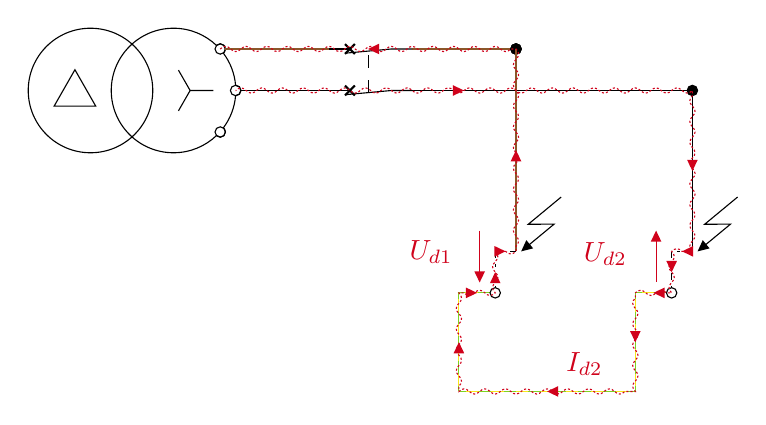
\begin{tikzpicture}[x=0.75pt,y=0.75pt,yscale=-1,xscale=1]
%uncomment if require: \path (0,219); %set diagram left start at 0, and has height of 219

%Straight Lines [id:da4511637283243949] 
\draw  [dash pattern={on 2.25pt off 2.25pt on 1pt off 2.25pt}]  (252.5,112.5) -- (242.5,112.5) -- (242.5,130) ;
%Straight Lines [id:da9527130819146642] 
\draw  [dash pattern={on 2.25pt off 2.25pt on 1pt off 2.25pt}]  (337.5,112.5) -- (327.5,112.5) -- (327.5,130) ;
%Straight Lines [id:da24126717784692808] 
\draw [color={rgb, 255:red, 0; green, 0; blue, 0 }  ,draw opacity=1 ]   (337.5,112.5) -- (337.5,35) ;
%Straight Lines [id:da3468467801372336] 
\draw    (202.5,35) -- (337.5,35) ;
%Straight Lines [id:da5563024891724297] 
\draw [color={rgb, 255:red, 139; green, 87; blue, 42 }  ,draw opacity=1 ]   (202.5,15) -- (252.5,15) ;
%Shape: Path Data [id:dp43837740322366014] 
\draw   (112.5,55) .. controls (112.5,56.38) and (111.38,57.5) .. (110,57.5) .. controls (109.29,57.5) and (108.65,57.2) .. (108.19,56.72) .. controls (102.81,61.85) and (95.52,65) .. (87.5,65) .. controls (70.93,65) and (57.5,51.57) .. (57.5,35) .. controls (57.5,18.43) and (70.93,5) .. (87.5,5) .. controls (95.52,5) and (102.81,8.15) .. (108.19,13.28) .. controls (108.65,12.8) and (109.29,12.5) .. (110,12.5) .. controls (111.38,12.5) and (112.5,13.62) .. (112.5,15) .. controls (112.5,15.82) and (112.11,16.54) .. (111.5,17) .. controls (114.8,21.39) and (116.92,26.71) .. (117.4,32.5) .. controls (117.43,32.5) and (117.47,32.5) .. (117.5,32.5) .. controls (118.88,32.5) and (120,33.62) .. (120,35) .. controls (120,36.38) and (118.88,37.5) .. (117.5,37.5) .. controls (117.47,37.5) and (117.43,37.5) .. (117.4,37.5) .. controls (116.92,43.29) and (114.8,48.61) .. (111.5,53) .. controls (112.11,53.46) and (112.5,54.18) .. (112.5,55) -- cycle ;
%Shape: Circle [id:dp03603482838008654] 
\draw   (17.5,35) .. controls (17.5,18.43) and (30.93,5) .. (47.5,5) .. controls (64.07,5) and (77.5,18.43) .. (77.5,35) .. controls (77.5,51.57) and (64.07,65) .. (47.5,65) .. controls (30.93,65) and (17.5,51.57) .. (17.5,35) -- cycle ;
%Shape: Triangle [id:dp7860018021593028] 
\draw   (40,25) -- (30,42.5) -- (50,42.5) -- cycle ;
%Shape: Star [id:dp36273195667205105] 
\draw   (106.75,35) -- (95.5,35) -- (89.88,44.81) -- (95.5,35) -- (89.88,25.19) -- (95.5,35) -- cycle ;
%Shape: Circle [id:dp581329576165861] 
\draw   (107.5,15) .. controls (107.5,13.62) and (108.62,12.5) .. (110,12.5) .. controls (111.38,12.5) and (112.5,13.62) .. (112.5,15) .. controls (112.5,16.38) and (111.38,17.5) .. (110,17.5) .. controls (108.62,17.5) and (107.5,16.38) .. (107.5,15) -- cycle ;
%Shape: Circle [id:dp008181652335233047] 
\draw   (114.9,35) .. controls (114.9,33.62) and (116.02,32.5) .. (117.4,32.5) .. controls (118.78,32.5) and (119.9,33.62) .. (119.9,35) .. controls (119.9,36.38) and (118.78,37.5) .. (117.4,37.5) .. controls (116.02,37.5) and (114.9,36.38) .. (114.9,35) -- cycle ;
%Shape: Circle [id:dp5428967410526352] 
\draw   (107.5,55) .. controls (107.5,53.62) and (108.62,52.5) .. (110,52.5) .. controls (111.38,52.5) and (112.5,53.62) .. (112.5,55) .. controls (112.5,56.38) and (111.38,57.5) .. (110,57.5) .. controls (108.62,57.5) and (107.5,56.38) .. (107.5,55) -- cycle ;

%Shape: Circle [id:dp3004196596154465] 
\draw  [fill={rgb, 255:red, 0; green, 0; blue, 0 }  ,fill opacity=1 ] (335,35) .. controls (335,33.62) and (336.12,32.5) .. (337.5,32.5) .. controls (338.88,32.5) and (340,33.62) .. (340,35) .. controls (340,36.38) and (338.88,37.5) .. (337.5,37.5) .. controls (336.12,37.5) and (335,36.38) .. (335,35) -- cycle ;
%Shape: Circle [id:dp38478162693673257] 
\draw  [fill={rgb, 255:red, 0; green, 0; blue, 0 }  ,fill opacity=1 ] (250,15) .. controls (250,13.62) and (251.12,12.5) .. (252.5,12.5) .. controls (253.88,12.5) and (255,13.62) .. (255,15) .. controls (255,16.38) and (253.88,17.5) .. (252.5,17.5) .. controls (251.12,17.5) and (250,16.38) .. (250,15) -- cycle ;
%Straight Lines [id:da35747201510733806] 
\draw [color={rgb, 255:red, 139; green, 87; blue, 42 }  ,draw opacity=1 ]   (112.5,15) -- (162.5,15) ;
%Straight Lines [id:da03938247690059582] 
\draw    (120,35) -- (162.5,35) ;
%Shape: Boxed Line [id:dp47312336425022783] 
\draw    (274.27,86.33) -- (258.39,99.47) -- (270.89,99.36) -- (257.31,110.59) ;
\draw [shift={(255,112.5)}, rotate = 320.40999999999997] [fill={rgb, 255:red, 0; green, 0; blue, 0 }  ][line width=0.08]  [draw opacity=0] (5.36,-2.57) -- (0,0) -- (5.36,2.57) -- cycle    ;
%Shape: Boxed Line [id:dp8604246706425941] 
\draw    (359.27,86.33) -- (343.39,99.47) -- (355.89,99.36) -- (342.31,110.59) ;
\draw [shift={(340,112.5)}, rotate = 320.40999999999997] [fill={rgb, 255:red, 0; green, 0; blue, 0 }  ][line width=0.08]  [draw opacity=0] (5.36,-2.57) -- (0,0) -- (5.36,2.57) -- cycle    ;
%Straight Lines [id:da6306782474143875] 
\draw    (170.5,37) -- (192.5,35) -- (202.5,35) ;
%Straight Lines [id:da4629224352649184] 
\draw    (172.5,35) -- (162.5,35) ;
\draw [shift={(172.5,35)}, rotate = 225] [color={rgb, 255:red, 0; green, 0; blue, 0 }  ][line width=0.75]    (-3.35,0) -- (3.35,0)(0,3.35) -- (0,-3.35)   ;
%Straight Lines [id:da5132783320552895] 
\draw    (170.5,17) -- (192.5,15) -- (202.5,15) ;
%Straight Lines [id:da123841191189479] 
\draw  [dash pattern={on 4.5pt off 4.5pt}]  (181.5,36) -- (181.5,16) ;
%Straight Lines [id:da38134434479229706] 
\draw    (172.5,15) -- (162.5,15) ;
\draw [shift={(172.5,15)}, rotate = 225] [color={rgb, 255:red, 0; green, 0; blue, 0 }  ][line width=0.75]    (-3.35,0) -- (3.35,0)(0,3.35) -- (0,-3.35)   ;

%Straight Lines [id:da029862379270012007] 
\draw [color={rgb, 255:red, 139; green, 87; blue, 42 }  ,draw opacity=1 ]   (252.5,112.5) -- (252.5,15) ;
%Shape: Circle [id:dp10157043967465573] 
\draw  [fill={rgb, 255:red, 0; green, 0; blue, 0 }  ,fill opacity=1 ] (250,15) .. controls (250,13.62) and (251.12,12.5) .. (252.5,12.5) .. controls (253.88,12.5) and (255,13.62) .. (255,15) .. controls (255,16.38) and (253.88,17.5) .. (252.5,17.5) .. controls (251.12,17.5) and (250,16.38) .. (250,15) -- cycle ;
%Shape: Circle [id:dp8079725241460669] 
\draw  [fill={rgb, 255:red, 0; green, 0; blue, 0 }  ,fill opacity=1 ] (250,15) .. controls (250,13.62) and (251.12,12.5) .. (252.5,12.5) .. controls (253.88,12.5) and (255,13.62) .. (255,15) .. controls (255,16.38) and (253.88,17.5) .. (252.5,17.5) .. controls (251.12,17.5) and (250,16.38) .. (250,15) -- cycle ;
%Straight Lines [id:da32787816985288987] 
\draw [color={rgb, 255:red, 208; green, 2; blue, 27 }  ,draw opacity=1 ]   (235,102.5) -- (235,124.5) ;
\draw [shift={(235,127.5)}, rotate = 270] [fill={rgb, 255:red, 208; green, 2; blue, 27 }  ,fill opacity=1 ][line width=0.08]  [draw opacity=0] (5.36,-2.57) -- (0,0) -- (5.36,2.57) -- cycle    ;
%Straight Lines [id:da9290035127505091] 
\draw [color={rgb, 255:red, 208; green, 2; blue, 27 }  ,draw opacity=1 ]   (320,105.5) -- (320,127.5) ;
\draw [shift={(320,102.5)}, rotate = 90] [fill={rgb, 255:red, 208; green, 2; blue, 27 }  ,fill opacity=1 ][line width=0.08]  [draw opacity=0] (5.36,-2.57) -- (0,0) -- (5.36,2.57) -- cycle    ;
%Straight Lines [id:da4236883272393758] 
\draw [color={rgb, 255:red, 248; green, 231; blue, 28 }  ,draw opacity=1 ]   (325,132.5) -- (310,132.5) -- (310,180) -- (225,180) ;
%Straight Lines [id:da1955939853197214] 
\draw [color={rgb, 255:red, 126; green, 211; blue, 33 }  ,draw opacity=1 ] [dash pattern={on 4.5pt off 4.5pt}]  (325,132.5) -- (310,132.5) -- (310,180) -- (225,180) ;
%Straight Lines [id:da8052192234703028] 
\draw [color={rgb, 255:red, 248; green, 231; blue, 28 }  ,draw opacity=1 ]   (240,132.5) -- (225,132.5) -- (225,180) ;
%Straight Lines [id:da6976347779102222] 
\draw [color={rgb, 255:red, 139; green, 87; blue, 42 }  ,draw opacity=1 ]   (252.5,110) -- (252.5,15) ;
%Straight Lines [id:da2970008681971681] 
\draw [color={rgb, 255:red, 126; green, 211; blue, 33 }  ,draw opacity=1 ] [dash pattern={on 4.5pt off 4.5pt}]  (240,132.5) -- (225,132.5) -- (225,180) ;
%Straight Lines [id:da7142618830255841] 
\draw [color={rgb, 255:red, 0; green, 0; blue, 0 }  ,draw opacity=1 ]   (337.5,110) -- (337.5,32.5) ;
%Shape: Circle [id:dp970057374964288] 
\draw  [fill={rgb, 255:red, 255; green, 255; blue, 255 }  ,fill opacity=1 ] (240,132.5) .. controls (240,131.12) and (241.12,130) .. (242.5,130) .. controls (243.88,130) and (245,131.12) .. (245,132.5) .. controls (245,133.88) and (243.88,135) .. (242.5,135) .. controls (241.12,135) and (240,133.88) .. (240,132.5) -- cycle ;
%Shape: Circle [id:dp5285112483449262] 
\draw  [fill={rgb, 255:red, 255; green, 255; blue, 255 }  ,fill opacity=1 ] (325,132.5) .. controls (325,131.12) and (326.12,130) .. (327.5,130) .. controls (328.88,130) and (330,131.12) .. (330,132.5) .. controls (330,133.88) and (328.88,135) .. (327.5,135) .. controls (326.12,135) and (325,133.88) .. (325,132.5) -- cycle ;
%Straight Lines [id:da2635484251048684] 
\draw [color={rgb, 255:red, 208; green, 2; blue, 27 }  ,draw opacity=1 ] [dash pattern={on 0.75pt off 0.75pt}]  (110,15) .. controls (111.67,13.33) and (113.33,13.33) .. (115,15) .. controls (116.67,16.67) and (118.33,16.67) .. (120,15) .. controls (121.67,13.33) and (123.33,13.33) .. (125,15) .. controls (126.67,16.67) and (128.33,16.67) .. (130,15) .. controls (131.67,13.33) and (133.33,13.33) .. (135,15) .. controls (136.67,16.67) and (138.33,16.67) .. (140,15) .. controls (141.67,13.33) and (143.33,13.33) .. (145,15) .. controls (146.67,16.67) and (148.33,16.67) .. (150,15) .. controls (151.67,13.33) and (153.33,13.33) .. (155,15) .. controls (156.67,16.67) and (158.33,16.67) .. (160,15) .. controls (161.67,13.33) and (163.33,13.33) .. (165,15) .. controls (166.67,16.67) and (168.33,16.67) .. (170,15) .. controls (171.67,13.33) and (173.33,13.33) .. (175,15) .. controls (176.67,16.67) and (178.33,16.67) .. (180,15) .. controls (181.67,13.33) and (183.33,13.33) .. (185,15) .. controls (186.67,16.67) and (188.33,16.67) .. (190,15) .. controls (191.67,13.33) and (193.33,13.33) .. (195,15) .. controls (196.67,16.67) and (198.33,16.67) .. (200,15) .. controls (201.67,13.33) and (203.33,13.33) .. (205,15) .. controls (206.67,16.67) and (208.33,16.67) .. (210,15) .. controls (211.67,13.33) and (213.33,13.33) .. (215,15) .. controls (216.67,16.67) and (218.33,16.67) .. (220,15) .. controls (221.67,13.33) and (223.33,13.33) .. (225,15) .. controls (226.67,16.67) and (228.33,16.67) .. (230,15) .. controls (231.67,13.33) and (233.33,13.33) .. (235,15) .. controls (236.67,16.67) and (238.33,16.67) .. (240,15) .. controls (241.67,13.33) and (243.33,13.33) .. (245,15) .. controls (246.67,16.67) and (248.33,16.67) .. (250,15) -- (252.5,15) -- (252.5,15) .. controls (254.17,16.67) and (254.17,18.33) .. (252.5,20) .. controls (250.83,21.67) and (250.83,23.33) .. (252.5,25) .. controls (254.17,26.67) and (254.17,28.33) .. (252.5,30) .. controls (250.83,31.67) and (250.83,33.33) .. (252.5,35) .. controls (254.17,36.67) and (254.17,38.33) .. (252.5,40) .. controls (250.83,41.67) and (250.83,43.33) .. (252.5,45) .. controls (254.17,46.67) and (254.17,48.33) .. (252.5,50) .. controls (250.83,51.67) and (250.83,53.33) .. (252.5,55) .. controls (254.17,56.67) and (254.17,58.33) .. (252.5,60) .. controls (250.83,61.67) and (250.83,63.33) .. (252.5,65) .. controls (254.17,66.67) and (254.17,68.33) .. (252.5,70) .. controls (250.83,71.67) and (250.83,73.33) .. (252.5,75) .. controls (254.17,76.67) and (254.17,78.33) .. (252.5,80) .. controls (250.83,81.67) and (250.83,83.33) .. (252.5,85) .. controls (254.17,86.67) and (254.17,88.33) .. (252.5,90) .. controls (250.83,91.67) and (250.83,93.33) .. (252.5,95) .. controls (254.17,96.67) and (254.17,98.33) .. (252.5,100) .. controls (250.83,101.67) and (250.83,103.33) .. (252.5,105) .. controls (254.17,106.67) and (254.17,108.33) .. (252.5,110) -- (252.5,112.5) -- (252.5,112.5) .. controls (250.83,114.17) and (249.17,114.17) .. (247.5,112.5) -- (242.5,112.5) -- (242.5,112.5) .. controls (244.17,114.17) and (244.17,115.83) .. (242.5,117.5) .. controls (240.83,119.17) and (240.83,120.83) .. (242.5,122.5) .. controls (244.17,124.17) and (244.17,125.83) .. (242.5,127.5) .. controls (240.83,129.17) and (240.83,130.83) .. (242.5,132.5) -- (242.5,132.5) .. controls (240.83,134.17) and (239.17,134.17) .. (237.5,132.5) .. controls (235.83,130.83) and (234.17,130.83) .. (232.5,132.5) .. controls (230.83,134.17) and (229.17,134.17) .. (227.5,132.5) -- (225,132.5) -- (225,132.5) .. controls (226.67,134.17) and (226.67,135.83) .. (225,137.5) .. controls (223.33,139.17) and (223.33,140.83) .. (225,142.5) .. controls (226.67,144.17) and (226.67,145.83) .. (225,147.5) .. controls (223.33,149.17) and (223.33,150.83) .. (225,152.5) .. controls (226.67,154.17) and (226.67,155.83) .. (225,157.5) .. controls (223.33,159.17) and (223.33,160.83) .. (225,162.5) .. controls (226.67,164.17) and (226.67,165.83) .. (225,167.5) .. controls (223.33,169.17) and (223.33,170.83) .. (225,172.5) .. controls (226.67,174.17) and (226.67,175.83) .. (225,177.5) -- (225,180) -- (225,180) .. controls (226.67,178.33) and (228.33,178.33) .. (230,180) .. controls (231.67,181.67) and (233.33,181.67) .. (235,180) .. controls (236.67,178.33) and (238.33,178.33) .. (240,180) .. controls (241.67,181.67) and (243.33,181.67) .. (245,180) .. controls (246.67,178.33) and (248.33,178.33) .. (250,180) .. controls (251.67,181.67) and (253.33,181.67) .. (255,180) .. controls (256.67,178.33) and (258.33,178.33) .. (260,180) .. controls (261.67,181.67) and (263.33,181.67) .. (265,180) .. controls (266.67,178.33) and (268.33,178.33) .. (270,180) .. controls (271.67,181.67) and (273.33,181.67) .. (275,180) .. controls (276.67,178.33) and (278.33,178.33) .. (280,180) .. controls (281.67,181.67) and (283.33,181.67) .. (285,180) .. controls (286.67,178.33) and (288.33,178.33) .. (290,180) .. controls (291.67,181.67) and (293.33,181.67) .. (295,180) .. controls (296.67,178.33) and (298.33,178.33) .. (300,180) .. controls (301.67,181.67) and (303.33,181.67) .. (305,180) -- (310,180) -- (310,180) .. controls (308.33,178.33) and (308.33,176.67) .. (310,175) .. controls (311.67,173.33) and (311.67,171.67) .. (310,170) .. controls (308.33,168.33) and (308.33,166.67) .. (310,165) .. controls (311.67,163.33) and (311.67,161.67) .. (310,160) .. controls (308.33,158.33) and (308.33,156.67) .. (310,155) .. controls (311.67,153.33) and (311.67,151.67) .. (310,150) .. controls (308.33,148.33) and (308.33,146.67) .. (310,145) .. controls (311.67,143.33) and (311.67,141.67) .. (310,140) .. controls (308.33,138.33) and (308.33,136.67) .. (310,135) -- (310,132.5) -- (310,132.5) .. controls (311.67,130.83) and (313.33,130.83) .. (315,132.5) .. controls (316.67,134.17) and (318.33,134.17) .. (320,132.5) .. controls (321.67,130.83) and (323.33,130.83) .. (325,132.5) -- (327.5,132.5) -- (327.5,132.5) .. controls (325.83,130.83) and (325.83,129.17) .. (327.5,127.5) .. controls (329.17,125.83) and (329.17,124.17) .. (327.5,122.5) .. controls (325.83,120.83) and (325.83,119.17) .. (327.5,117.5) .. controls (329.17,115.83) and (329.17,114.17) .. (327.5,112.5) -- (327.5,112.5) .. controls (329.17,110.83) and (330.83,110.83) .. (332.5,112.5) -- (337.5,112.5) -- (337.5,112.5) .. controls (335.83,110.83) and (335.83,109.17) .. (337.5,107.5) .. controls (339.17,105.83) and (339.17,104.17) .. (337.5,102.5) .. controls (335.83,100.83) and (335.83,99.17) .. (337.5,97.5) .. controls (339.17,95.83) and (339.17,94.17) .. (337.5,92.5) .. controls (335.83,90.83) and (335.83,89.17) .. (337.5,87.5) .. controls (339.17,85.83) and (339.17,84.17) .. (337.5,82.5) .. controls (335.83,80.83) and (335.83,79.17) .. (337.5,77.5) .. controls (339.17,75.83) and (339.17,74.17) .. (337.5,72.5) .. controls (335.83,70.83) and (335.83,69.17) .. (337.5,67.5) .. controls (339.17,65.83) and (339.17,64.17) .. (337.5,62.5) .. controls (335.83,60.83) and (335.83,59.17) .. (337.5,57.5) .. controls (339.17,55.83) and (339.17,54.17) .. (337.5,52.5) .. controls (335.83,50.83) and (335.83,49.17) .. (337.5,47.5) .. controls (339.17,45.83) and (339.17,44.17) .. (337.5,42.5) .. controls (335.83,40.83) and (335.83,39.17) .. (337.5,37.5) -- (337.5,35) -- (337.5,35) .. controls (335.83,36.67) and (334.17,36.67) .. (332.5,35) .. controls (330.83,33.33) and (329.17,33.33) .. (327.5,35) .. controls (325.83,36.67) and (324.17,36.67) .. (322.5,35) .. controls (320.83,33.33) and (319.17,33.33) .. (317.5,35) .. controls (315.83,36.67) and (314.17,36.67) .. (312.5,35) .. controls (310.83,33.33) and (309.17,33.33) .. (307.5,35) .. controls (305.83,36.67) and (304.17,36.67) .. (302.5,35) .. controls (300.83,33.33) and (299.17,33.33) .. (297.5,35) .. controls (295.83,36.67) and (294.17,36.67) .. (292.5,35) .. controls (290.83,33.33) and (289.17,33.33) .. (287.5,35) .. controls (285.83,36.67) and (284.17,36.67) .. (282.5,35) .. controls (280.83,33.33) and (279.17,33.33) .. (277.5,35) .. controls (275.83,36.67) and (274.17,36.67) .. (272.5,35) .. controls (270.83,33.33) and (269.17,33.33) .. (267.5,35) .. controls (265.83,36.67) and (264.17,36.67) .. (262.5,35) .. controls (260.83,33.33) and (259.17,33.33) .. (257.5,35) .. controls (255.83,36.67) and (254.17,36.67) .. (252.5,35) .. controls (250.83,33.33) and (249.17,33.33) .. (247.5,35) .. controls (245.83,36.67) and (244.17,36.67) .. (242.5,35) .. controls (240.83,33.33) and (239.17,33.33) .. (237.5,35) .. controls (235.83,36.67) and (234.17,36.67) .. (232.5,35) .. controls (230.83,33.33) and (229.17,33.33) .. (227.5,35) .. controls (225.83,36.67) and (224.17,36.67) .. (222.5,35) .. controls (220.83,33.33) and (219.17,33.33) .. (217.5,35) .. controls (215.83,36.67) and (214.17,36.67) .. (212.5,35) .. controls (210.83,33.33) and (209.17,33.33) .. (207.5,35) .. controls (205.83,36.67) and (204.17,36.67) .. (202.5,35) .. controls (200.83,33.33) and (199.17,33.33) .. (197.5,35) .. controls (195.83,36.67) and (194.17,36.67) .. (192.5,35) .. controls (190.83,33.33) and (189.17,33.33) .. (187.5,35) .. controls (185.83,36.67) and (184.17,36.67) .. (182.5,35) .. controls (180.83,33.33) and (179.17,33.33) .. (177.5,35) .. controls (175.83,36.67) and (174.17,36.67) .. (172.5,35) .. controls (170.83,33.33) and (169.17,33.33) .. (167.5,35) .. controls (165.83,36.67) and (164.17,36.67) .. (162.5,35) .. controls (160.83,33.33) and (159.17,33.33) .. (157.5,35) .. controls (155.83,36.67) and (154.17,36.67) .. (152.5,35) .. controls (150.83,33.33) and (149.17,33.33) .. (147.5,35) .. controls (145.83,36.67) and (144.17,36.67) .. (142.5,35) .. controls (140.83,33.33) and (139.17,33.33) .. (137.5,35) .. controls (135.83,36.67) and (134.17,36.67) .. (132.5,35) .. controls (130.83,33.33) and (129.17,33.33) .. (127.5,35) .. controls (125.83,36.67) and (124.17,36.67) .. (122.5,35) .. controls (120.83,33.33) and (119.17,33.33) .. (117.5,35) -- (117.4,35) -- (117.4,35) ;
\draw [shift={(181.25,15)}, rotate = 0] [fill={rgb, 255:red, 208; green, 2; blue, 27 }  ,fill opacity=1 ][line width=0.08]  [draw opacity=0] (5.36,-2.57) -- (0,0) -- (5.36,2.57) -- cycle    ;
\draw [shift={(252.5,63.75)}, rotate = 90] [fill={rgb, 255:red, 208; green, 2; blue, 27 }  ,fill opacity=1 ][line width=0.08]  [draw opacity=0] (5.36,-2.57) -- (0,0) -- (5.36,2.57) -- cycle    ;
\draw [shift={(247.5,112.5)}, rotate = 180] [fill={rgb, 255:red, 208; green, 2; blue, 27 }  ,fill opacity=1 ][line width=0.08]  [draw opacity=0] (5.36,-2.57) -- (0,0) -- (5.36,2.57) -- cycle    ;
\draw [shift={(242.5,122.5)}, rotate = 90] [fill={rgb, 255:red, 208; green, 2; blue, 27 }  ,fill opacity=1 ][line width=0.08]  [draw opacity=0] (5.36,-2.57) -- (0,0) -- (5.36,2.57) -- cycle    ;
\draw [shift={(233.75,132.5)}, rotate = 180] [fill={rgb, 255:red, 208; green, 2; blue, 27 }  ,fill opacity=1 ][line width=0.08]  [draw opacity=0] (5.36,-2.57) -- (0,0) -- (5.36,2.57) -- cycle    ;
\draw [shift={(225,156.25)}, rotate = 90] [fill={rgb, 255:red, 208; green, 2; blue, 27 }  ,fill opacity=1 ][line width=0.08]  [draw opacity=0] (5.36,-2.57) -- (0,0) -- (5.36,2.57) -- cycle    ;
\draw [shift={(267.5,180)}, rotate = 0] [fill={rgb, 255:red, 208; green, 2; blue, 27 }  ,fill opacity=1 ][line width=0.08]  [draw opacity=0] (5.36,-2.57) -- (0,0) -- (5.36,2.57) -- cycle    ;
\draw [shift={(310,156.25)}, rotate = 270] [fill={rgb, 255:red, 208; green, 2; blue, 27 }  ,fill opacity=1 ][line width=0.08]  [draw opacity=0] (5.36,-2.57) -- (0,0) -- (5.36,2.57) -- cycle    ;
\draw [shift={(318.75,132.5)}, rotate = 0] [fill={rgb, 255:red, 208; green, 2; blue, 27 }  ,fill opacity=1 ][line width=0.08]  [draw opacity=0] (5.36,-2.57) -- (0,0) -- (5.36,2.57) -- cycle    ;
\draw [shift={(327.5,122.5)}, rotate = 270] [fill={rgb, 255:red, 208; green, 2; blue, 27 }  ,fill opacity=1 ][line width=0.08]  [draw opacity=0] (5.36,-2.57) -- (0,0) -- (5.36,2.57) -- cycle    ;
\draw [shift={(332.5,112.5)}, rotate = 0] [fill={rgb, 255:red, 208; green, 2; blue, 27 }  ,fill opacity=1 ][line width=0.08]  [draw opacity=0] (5.36,-2.57) -- (0,0) -- (5.36,2.57) -- cycle    ;
\draw [shift={(337.5,73.75)}, rotate = 270] [fill={rgb, 255:red, 208; green, 2; blue, 27 }  ,fill opacity=1 ][line width=0.08]  [draw opacity=0] (5.36,-2.57) -- (0,0) -- (5.36,2.57) -- cycle    ;
\draw [shift={(227.45,35)}, rotate = 180] [fill={rgb, 255:red, 208; green, 2; blue, 27 }  ,fill opacity=1 ][line width=0.08]  [draw opacity=0] (5.36,-2.57) -- (0,0) -- (5.36,2.57) -- cycle    ;


% Text Node
\draw (275.5,160) node [anchor=north west][inner sep=0.75pt]  [color={rgb, 255:red, 208; green, 2; blue, 27 }  ,opacity=1 ] [align=left] {$I_{d2}$};
% Text Node
\draw (200,106) node [anchor=north west][inner sep=0.75pt]  [color={rgb, 255:red, 208; green, 2; blue, 27 }  ,opacity=1 ] [align=left] {$U_{d1}$};
% Text Node
\draw (284,107) node [anchor=north west][inner sep=0.75pt]  [color={rgb, 255:red, 208; green, 2; blue, 27 }  ,opacity=1 ] [align=left] {$U_{d2}$};


\end{tikzpicture}


\end{figure}

%\end{document}


L'intensité de courant $I_{d2}$ vaut alors :
\begin{formule}{Courant du deuxième défaut $I_{d2}$ en schéma Isolé-Interconnecté}{}
\begin{align*}
		I_{d2} &= \frac{0,5 \times U}{R_{ph1}+R_{ph2}} \\
\end{align*}

\begin{textvariables}
U								& tension nominale composée				& volt			& \volt					& 	Différence de potentiel entre deux conducteurs actifs (à préciser s'il s'agit du conducteur neutre)	\\
R_{ph1}					& résistance											& ohm			& \ohm					& 	Résistance de du conducteur actif alimentant l'appareil 1\\
R_{ph2}					& résistance											& ohm			& \ohm					& 	Résistance de du conducteur actif alimentant l'appareil 2\\
\end{textvariables}
\end{formule}

Le courant de défaut $I_{d1}$ fera alors apparaître une \emph{tension de défaut} $U_{d}$ entre la masse métallique de l'appareil 1 et la masse métallique de l'appareil 2. \\
On néglige également la résistance du conducteur PE devant celle des phases. Dans ce contexte-là, la tension de défaut $U_d$ vaut alors :

\begin{formule}{Tension de défaut $U_{d}$ en schéma Isolé-Individuel}{}
\begin{align*}
		U_{d} &= \frac{0,5 \times U}{2} \\
\end{align*}

\begin{textvariables}
U								& tension nominale composée				& volt			& \volt					& 	Différence de potentiel entre deux conducteurs actifs (à préciser s'il s'agit du conducteur neutre)	\\
I_{d2}						& intensité												& ampère		& \ampere				& 	Courant de défaut de l'appareil 2 \\
U_{L}						& tension							& volt			& \volt										& 	Tension de sécurité du local avec :
\begin{description}[nosep, leftmargin=*]
\item[Local sec :] $U_{L}=\SI{50}{\volt}$
\item[Local humide :] $U_{L}=\SI{25}{\volt}$
\end{description} \\
\end{textvariables}
\end{formule}

Cette tension de défaut est dangereuse et il faut obligatoirement couper l'alimentation en protégeant les circuits par des disjoncteurs magnéto-thermiques, qui doivent respecter les temps de coupure suivants :

%--------------------------------------
%ELECTROTECHNIQUE - SCHEMA DE LIAISON A LA TERRE
%--------------------------------------

%utiliser les environnement \begin{comment} \end{comment} pour mettre en commentaire le préambule une fois la programmation appelée dans le document maître (!ne pas oublier de mettre en commentaire \end{document}!)

\begin{comment}

\documentclass[a4paper, 11pt, twoside, fleqn]{memoir}

\usepackage{AOCDTF}

\marqueurchapitre
\decoupagechapitre{1} %juste pour éviter les erreurs lors de la compilation des sous-programmations (passera en commentaire)

%lien d'édition des figures Tikz sur le site mathcha.io (rajouter le lien d'une modification effectuée sur la figure tikz avec le nom du modificateur car il n'y a qu'un lien par compte)

%lien éditeur Bruno Douchy : https://www.mathcha.io/editor/zjygnFElSdyhJ72e3zT5ZgqwBT4DKnovswpXn1q

%--------------------------------------
%corps du document
%--------------------------------------

\begin{document} %corps du document
	\openleft %début de chapitre à gauche

\end{comment}

\begin{table}[H]
\caption{Temps de coupure maximal des disjoncteurs en schéma IT\label{tab:schema_it_temps_coupure}}
\begin{threeparttable} %note dans tableau
\begin{tabularx}{\textwidth}{C C C}
\toprule
\multirow[c]{2}{*}{\thead{Réseaux usuels}} & \multicolumn{2}{c}{\thead{Temps de coupure maximal (\si{\milli\second})}}\\
\cmidrule(lr){2-3} 
	& $U_{L}=\SI{50}{\volt}$ 	& 			$U_{L}=\SI{25}{\volt}$  \\
\midrule
\multicolumn{3}{l}{Neutre non distribué} \\
\middashrule
\SI{127}{\volt}/\SI{230}{\volt}		& 800		& 400 \\
\SI{230}{\volt}/\SI{400}{\volt}		& 400		& 200 \\
\SI{400}{\volt}/\SI{690}{\volt}		& 200		& 60 \\
\SI{690}{\volt}/\SI{1000}{\volt}	& 100		& 20 \\
\addlinespace
\multicolumn{3}{l}{Neutre distribué\tnote{1}} \\
\middashrule
\SI{127}{\volt}/\SI{230}{\volt}		& 5000		& 1000 \\
\SI{230}{\volt}/\SI{400}{\volt}		& 800		& 500 \\
\SI{400}{\volt}/\SI{690}{\volt}		& 400		& 200 \\
\SI{690}{\volt}/\SI{1000}{\volt}	& 200		& 80 \\
\bottomrule 
\end{tabularx}
\begin{tablenotes}
    \item[1] les installations monophasées sont considérées comme des installations à neutre distribué.
\end{tablenotes}
\end{threeparttable} %note dans tableau
\end{table}

%\end{document}



La longueur maximale des conducteurs en schéma IT avec les masses interconnectées se calcule avec les mêmes méthodes que pour les installations en schéma TN (voir \superref{sec:schema_tn_methode_conventionnelle}).

\section{Contrôle permanent de l'installation en schéma IT}

Quand l'installation électrique est en schéma IT, il est nécessaire d'avoir une équipe de maintenance à disposition pour intervenir rapidement en cas de premier défaut. Pour les détecter au plus vite, il faut installer un Contrôleur Permanent d'Isolement (CPI). Il s'agit d'un appareil placé en dérivation qui va calculer en permanence deux paramètres de l'installation :
\begin{description}
\item[\Circled{1} niveau d'isolement général $Z_{res}$ :] injection d'une tension (continue ou alternative de basse fréquence) entre le neutre et la terre, générant un \emph{courant de fuite} $I_f$ dont l'intensité sera proportionnellement inverse au niveau d'isolement général de l'installation électrique. Au-dessous d'un certain seuil d'isolement réglable (généralement entre \numrange{0,7}{100}\si{\kilo\ohm}), le CPI déclenche une alarme. 
\item[\Circled{2} apparition d'un défaut franc sur un circuit :] installation de tores de détection sur les circuits à surveiller, calculant la différence entre le courant entre et sortant (mécanisme similaire à ceux des DDR). Cela permet de localiser précisément les circuits en défaut.
\end{description} 

 \begin{figure}[H]
\caption{Installation Isolé-Individuelle avec CPI}
\begin{subfigure}[t]{0.49\linewidth}
%--------------------------------------
%ELECTROTECHNIQUE - SCHEMA DE LIAISON A LA TERRE
%--------------------------------------

%utiliser les environnement \begin{comment} \end{comment} pour mettre en commentaire le préambule une fois la programmation appelée dans le document maître (!ne pas oublier de mettre en commentaire \end{document}!)

\begin{comment}

\documentclass[a4paper, 11pt, twoside, fleqn]{memoir}

\usepackage{AOCDTF}

\marqueurchapitre
\decoupagechapitre{1} %juste pour éviter les erreurs lors de la compilation des sous-programmations (passera en commentaire)

%lien d'édition des figures Tikz sur le site mathcha.io (rajouter le lien d'une modification effectuée sur la figure tikz avec le nom du modificateur car il n'y a qu'un lien par compte)

%lien mathcha Bruno Douchy : https://www.mathcha.io/editor/jQKLoCODsYQuv6lo9wh5LQq3pSzO0mydSnpzwBy

%--------------------------------------
%corps du document
%--------------------------------------

\begin{document} %corps du document
	\openleft %début de chapitre à gauche

\end{comment}



% Pattern Info
 
\tikzset{
pattern size/.store in=\mcSize, 
pattern size = 5pt,
pattern thickness/.store in=\mcThickness, 
pattern thickness = 0.3pt,
pattern radius/.store in=\mcRadius, 
pattern radius = 1pt}
\makeatletter
\pgfutil@ifundefined{pgf@pattern@name@_2ybrnrdqo}{
\pgfdeclarepatternformonly[\mcThickness,\mcSize]{_2ybrnrdqo}
{\pgfqpoint{0pt}{0pt}}
{\pgfpoint{\mcSize+\mcThickness}{\mcSize+\mcThickness}}
{\pgfpoint{\mcSize}{\mcSize}}
{
\pgfsetcolor{\tikz@pattern@color}
\pgfsetlinewidth{\mcThickness}
\pgfpathmoveto{\pgfqpoint{0pt}{0pt}}
\pgfpathlineto{\pgfpoint{\mcSize+\mcThickness}{\mcSize+\mcThickness}}
\pgfusepath{stroke}
}}
\makeatother
\tikzset{every picture/.style={line width=0.5pt}} %set default line width to 0.75pt        

\begin{tikzpicture}[x=0.75pt,y=0.75pt,yscale=-0.6,xscale=0.6]
%uncomment if require: \path (0,320); %set diagram left start at 0, and has height of 320

%Straight Lines [id:da4922757986185987] 
\draw [color={rgb, 255:red, 74; green, 144; blue, 226 }  ,draw opacity=1 ]   (152.5,75) -- (162.5,75) ;
%Straight Lines [id:da4038713220143262] 
\draw [color={rgb, 255:red, 74; green, 144; blue, 226 }  ,draw opacity=1 ]   (462.5,175) -- (462.5,155) ;
%Straight Lines [id:da9166454765790462] 
\draw [color={rgb, 255:red, 74; green, 144; blue, 226 }  ,draw opacity=1 ]   (462.5,107.5) -- (462.5,77.5) ;
%Straight Lines [id:da9023577986083069] 
\draw [color={rgb, 255:red, 74; green, 144; blue, 226 }  ,draw opacity=1 ]   (377.5,175) -- (377.5,155) ;
%Straight Lines [id:da5928803977736146] 
\draw [color={rgb, 255:red, 74; green, 144; blue, 226 }  ,draw opacity=1 ]   (377.5,107.5) -- (377.5,77.5) ;
%Straight Lines [id:da30570583399348505] 
\draw [color={rgb, 255:red, 74; green, 144; blue, 226 }  ,draw opacity=1 ]   (292.5,175) -- (292.5,155) ;
%Straight Lines [id:da8819404575351564] 
\draw [color={rgb, 255:red, 139; green, 87; blue, 42 }  ,draw opacity=1 ]   (252.5,175) -- (252.5,155) ;
%Straight Lines [id:da28367841763640167] 
\draw [color={rgb, 255:red, 155; green, 155; blue, 155 }  ,draw opacity=1 ]   (422.5,175) -- (422.5,155) ;
%Straight Lines [id:da6880263813112385] 
\draw [color={rgb, 255:red, 0; green, 0; blue, 0 }  ,draw opacity=1 ]   (337.5,175) -- (337.5,152.5) ;
%Straight Lines [id:da8972215794381513] 
\draw [color={rgb, 255:red, 248; green, 231; blue, 28 }  ,draw opacity=1 ]   (87.5,75) -- (27.5,75) -- (27.5,182.5) ;
%Straight Lines [id:da07998178544200962] 
\draw [color={rgb, 255:red, 248; green, 231; blue, 28 }  ,draw opacity=1 ]   (95.5,35) -- (87.5,75) -- (87.5,107.5) ;
%Straight Lines [id:da7929766229120194] 
\draw [color={rgb, 255:red, 126; green, 211; blue, 33 }  ,draw opacity=1 ] [dash pattern={on 2.25pt off 2.25pt}]  (95.5,35) -- (87.5,75) -- (87.5,107.5) ;
%Straight Lines [id:da4949912109010227] 
\draw [color={rgb, 255:red, 74; green, 144; blue, 226 }  ,draw opacity=1 ]   (202.5,75) -- (460,75) ;
%Straight Lines [id:da7560950775201385] 
\draw [color={rgb, 255:red, 248; green, 231; blue, 28 }  ,draw opacity=1 ]   (240,180) -- (225,180) -- (225,182.5) ;
%Straight Lines [id:da49944531942669546] 
\draw    (202.5,35) -- (462.5,35) ;
%Straight Lines [id:da47196191445949953] 
\draw [color={rgb, 255:red, 139; green, 87; blue, 42 }  ,draw opacity=1 ]   (202.5,15) -- (462.5,15) ;
%Straight Lines [id:da034038054075003044] 
\draw [color={rgb, 255:red, 155; green, 155; blue, 155 }  ,draw opacity=1 ]   (202.5,55) -- (462.5,55) ;
%Shape: Path Data [id:dp09879682351014718] 
\draw   (112.5,55) .. controls (112.5,56.38) and (111.38,57.5) .. (110,57.5) .. controls (109.29,57.5) and (108.65,57.2) .. (108.19,56.72) .. controls (102.81,61.85) and (95.52,65) .. (87.5,65) .. controls (70.93,65) and (57.5,51.57) .. (57.5,35) .. controls (57.5,18.43) and (70.93,5) .. (87.5,5) .. controls (95.52,5) and (102.81,8.15) .. (108.19,13.28) .. controls (108.65,12.8) and (109.29,12.5) .. (110,12.5) .. controls (111.38,12.5) and (112.5,13.62) .. (112.5,15) .. controls (112.5,15.82) and (112.11,16.54) .. (111.5,17) .. controls (114.8,21.39) and (116.92,26.71) .. (117.4,32.5) .. controls (117.43,32.5) and (117.47,32.5) .. (117.5,32.5) .. controls (118.88,32.5) and (120,33.62) .. (120,35) .. controls (120,36.38) and (118.88,37.5) .. (117.5,37.5) .. controls (117.47,37.5) and (117.43,37.5) .. (117.4,37.5) .. controls (116.92,43.29) and (114.8,48.61) .. (111.5,53) .. controls (112.11,53.46) and (112.5,54.18) .. (112.5,55) -- cycle ;
%Shape: Circle [id:dp09395491014356527] 
\draw   (17.5,35) .. controls (17.5,18.43) and (30.93,5) .. (47.5,5) .. controls (64.07,5) and (77.5,18.43) .. (77.5,35) .. controls (77.5,51.57) and (64.07,65) .. (47.5,65) .. controls (30.93,65) and (17.5,51.57) .. (17.5,35) -- cycle ;
%Shape: Triangle [id:dp01558250765431457] 
\draw   (40,25) -- (30,42.5) -- (50,42.5) -- cycle ;
%Shape: Star [id:dp0013707252732991781] 
\draw   (106.75,35) -- (95.5,35) -- (89.88,44.81) -- (95.5,35) -- (89.88,25.19) -- (95.5,35) -- cycle ;
%Shape: Circle [id:dp39893592802184263] 
\draw   (107.5,15) .. controls (107.5,13.62) and (108.62,12.5) .. (110,12.5) .. controls (111.38,12.5) and (112.5,13.62) .. (112.5,15) .. controls (112.5,16.38) and (111.38,17.5) .. (110,17.5) .. controls (108.62,17.5) and (107.5,16.38) .. (107.5,15) -- cycle ;
%Shape: Circle [id:dp9893284041115082] 
\draw   (114.9,35) .. controls (114.9,33.62) and (116.02,32.5) .. (117.4,32.5) .. controls (118.78,32.5) and (119.9,33.62) .. (119.9,35) .. controls (119.9,36.38) and (118.78,37.5) .. (117.4,37.5) .. controls (116.02,37.5) and (114.9,36.38) .. (114.9,35) -- cycle ;
%Shape: Circle [id:dp3917292266620266] 
\draw   (107.5,55) .. controls (107.5,53.62) and (108.62,52.5) .. (110,52.5) .. controls (111.38,52.5) and (112.5,53.62) .. (112.5,55) .. controls (112.5,56.38) and (111.38,57.5) .. (110,57.5) .. controls (108.62,57.5) and (107.5,56.38) .. (107.5,55) -- cycle ;

%Straight Lines [id:da8322026187642189] 
\draw [color={rgb, 255:red, 139; green, 87; blue, 42 }  ,draw opacity=1 ]   (252.5,107.5) -- (252.5,15) ;
%Straight Lines [id:da8041249564118628] 
\draw [color={rgb, 255:red, 74; green, 144; blue, 226 }  ,draw opacity=1 ]   (292.5,107.5) -- (292.5,77.5) ;
%Straight Lines [id:da6342365727576158] 
\draw    (17.5,232.5) -- (460,232.5) ;
%Shape: Rectangle [id:dp8835182839666373] 
\draw  [draw opacity=0][pattern=_2ybrnrdqo,pattern size=6pt,pattern thickness=0.75pt,pattern radius=0pt, pattern color={rgb, 255:red, 0; green, 0; blue, 0}][line width=0.75]  (17.5,232.5) -- (460,232.5) -- (460,247.5) -- (17.5,247.5) -- cycle ;
%Straight Lines [id:da658767187431958] 
\draw [color={rgb, 255:red, 126; green, 211; blue, 33 }  ,draw opacity=1 ] [dash pattern={on 2.25pt off 2.25pt}]  (240,180) -- (225,180) -- (225,182.5) ;
%Straight Lines [id:da06637251377195108] 
\draw [color={rgb, 255:red, 248; green, 231; blue, 28 }  ,draw opacity=1 ]   (225,222.5) -- (225,247.5) ;
%Straight Lines [id:da47233881321451787] 
\draw    (225,247.5) -- (225,262.5) ;
%Straight Lines [id:da5035312706678949] 
\draw    (215,262.5) -- (235,262.5) ;
%Straight Lines [id:da18116556144696694] 
\draw    (217.5,267.5) -- (232.5,267.5) ;
%Straight Lines [id:da26663321343914415] 
\draw    (220,272.5) -- (230,272.5) ;

%Straight Lines [id:da7788639142047531] 
\draw [color={rgb, 255:red, 126; green, 211; blue, 33 }  ,draw opacity=1 ] [dash pattern={on 2.25pt off 2.25pt}]  (225,222.5) -- (225,247.5) ;
%Straight Lines [id:da8201802660928923] 
\draw    (287.5,175) -- (292.5,175) ;
%Shape: Rectangle [id:dp3438336194943209] 
\draw   (257.5,170) -- (287.5,170) -- (287.5,180) -- (257.5,180) -- cycle ;
%Straight Lines [id:da27605197781986657] 
\draw    (252.5,175) -- (257.5,175) ;

%Straight Lines [id:da9011697570747588] 
\draw    (225,217.5) -- (225,222.5) ;
%Shape: Rectangle [id:dp36989703847460553] 
\draw   (230,187.5) -- (230,217.5) -- (220,217.5) -- (220,187.5) -- cycle ;
%Straight Lines [id:da6366900985555619] 
\draw    (225,182.5) -- (225,187.5) ;

%Straight Lines [id:da3812281827541767] 
\draw [color={rgb, 255:red, 0; green, 0; blue, 0 }  ,draw opacity=1 ]   (337.5,107.5) -- (337.5,37.5) ;
%Straight Lines [id:da02888103671964104] 
\draw    (372.5,175) -- (377.5,175) ;
%Shape: Rectangle [id:dp39971735208919124] 
\draw   (342.5,170) -- (372.5,170) -- (372.5,180) -- (342.5,180) -- cycle ;
%Straight Lines [id:da15610963345624862] 
\draw    (337.5,175) -- (342.5,175) ;

%Straight Lines [id:da7566594469565104] 
\draw [color={rgb, 255:red, 155; green, 155; blue, 155 }  ,draw opacity=1 ]   (422.5,107.5) -- (422.5,57.5) ;
%Straight Lines [id:da9791907804470615] 
\draw [color={rgb, 255:red, 74; green, 144; blue, 226 }  ,draw opacity=1 ]   (462.5,175.5) -- (462.5,162.5) ;
%Straight Lines [id:da15543680976570695] 
\draw    (457.5,175) -- (462.5,175) ;
%Shape: Rectangle [id:dp27259637225024935] 
\draw   (427.5,170) -- (457.5,170) -- (457.5,180) -- (427.5,180) -- cycle ;
%Straight Lines [id:da6590266150100259] 
\draw    (422.5,175) -- (427.5,175) ;

%Shape: Circle [id:dp3040137945437842] 
\draw  [fill={rgb, 255:red, 0; green, 0; blue, 0 }  ,fill opacity=1 ] (375,75) .. controls (375,73.62) and (376.12,72.5) .. (377.5,72.5) .. controls (378.88,72.5) and (380,73.62) .. (380,75) .. controls (380,76.38) and (378.88,77.5) .. (377.5,77.5) .. controls (376.12,77.5) and (375,76.38) .. (375,75) -- cycle ;
%Shape: Circle [id:dp5886475323071111] 
\draw  [fill={rgb, 255:red, 0; green, 0; blue, 0 }  ,fill opacity=1 ] (460,75) .. controls (460,73.62) and (461.12,72.5) .. (462.5,72.5) .. controls (463.88,72.5) and (465,73.62) .. (465,75) .. controls (465,76.38) and (463.88,77.5) .. (462.5,77.5) .. controls (461.12,77.5) and (460,76.38) .. (460,75) -- cycle ;
%Shape: Circle [id:dp7341854734672731] 
\draw  [fill={rgb, 255:red, 0; green, 0; blue, 0 }  ,fill opacity=1 ] (335,35) .. controls (335,33.62) and (336.12,32.5) .. (337.5,32.5) .. controls (338.88,32.5) and (340,33.62) .. (340,35) .. controls (340,36.38) and (338.88,37.5) .. (337.5,37.5) .. controls (336.12,37.5) and (335,36.38) .. (335,35) -- cycle ;
%Shape: Circle [id:dp6336551833672776] 
\draw  [fill={rgb, 255:red, 0; green, 0; blue, 0 }  ,fill opacity=1 ] (420,55) .. controls (420,53.62) and (421.12,52.5) .. (422.5,52.5) .. controls (423.88,52.5) and (425,53.62) .. (425,55) .. controls (425,56.38) and (423.88,57.5) .. (422.5,57.5) .. controls (421.12,57.5) and (420,56.38) .. (420,55) -- cycle ;
%Shape: Circle [id:dp5716316243984012] 
\draw  [fill={rgb, 255:red, 0; green, 0; blue, 0 }  ,fill opacity=1 ] (290,75) .. controls (290,73.62) and (291.12,72.5) .. (292.5,72.5) .. controls (293.88,72.5) and (295,73.62) .. (295,75) .. controls (295,76.38) and (293.88,77.5) .. (292.5,77.5) .. controls (291.12,77.5) and (290,76.38) .. (290,75) -- cycle ;
%Shape: Circle [id:dp9134099794169516] 
\draw  [fill={rgb, 255:red, 0; green, 0; blue, 0 }  ,fill opacity=1 ] (250,15) .. controls (250,13.62) and (251.12,12.5) .. (252.5,12.5) .. controls (253.88,12.5) and (255,13.62) .. (255,15) .. controls (255,16.38) and (253.88,17.5) .. (252.5,17.5) .. controls (251.12,17.5) and (250,16.38) .. (250,15) -- cycle ;
%Shape: Rectangle [id:dp9736059741519228] 
\draw  [dash pattern={on 2.25pt off 2.25pt on 1pt off 2.25pt}] (242.5,160) -- (302.5,160) -- (302.5,190) -- (242.5,190) -- cycle ;
%Shape: Circle [id:dp314574850816974] 
\draw  [fill={rgb, 255:red, 255; green, 255; blue, 255 }  ,fill opacity=1 ] (240,180) .. controls (240,178.62) and (241.12,177.5) .. (242.5,177.5) .. controls (243.88,177.5) and (245,178.62) .. (245,180) .. controls (245,181.38) and (243.88,182.5) .. (242.5,182.5) .. controls (241.12,182.5) and (240,181.38) .. (240,180) -- cycle ;
%Shape: Circle [id:dp27575875918191606] 
\draw  [fill={rgb, 255:red, 255; green, 255; blue, 255 }  ,fill opacity=1 ] (250,160) .. controls (250,158.62) and (251.12,157.5) .. (252.5,157.5) .. controls (253.88,157.5) and (255,158.62) .. (255,160) .. controls (255,161.38) and (253.88,162.5) .. (252.5,162.5) .. controls (251.12,162.5) and (250,161.38) .. (250,160) -- cycle ;
%Shape: Circle [id:dp7954116399024105] 
\draw  [fill={rgb, 255:red, 255; green, 255; blue, 255 }  ,fill opacity=1 ] (290,160) .. controls (290,158.62) and (291.12,157.5) .. (292.5,157.5) .. controls (293.88,157.5) and (295,158.62) .. (295,160) .. controls (295,161.38) and (293.88,162.5) .. (292.5,162.5) .. controls (291.12,162.5) and (290,161.38) .. (290,160) -- cycle ;
%Shape: Rectangle [id:dp6541068284877478] 
\draw  [dash pattern={on 2.25pt off 2.25pt on 1pt off 2.25pt}] (327.5,160) -- (387.5,160) -- (387.5,190) -- (327.5,190) -- cycle ;
%Shape: Circle [id:dp018941541358536207] 
\draw  [fill={rgb, 255:red, 255; green, 255; blue, 255 }  ,fill opacity=1 ] (335,160) .. controls (335,158.62) and (336.12,157.5) .. (337.5,157.5) .. controls (338.88,157.5) and (340,158.62) .. (340,160) .. controls (340,161.38) and (338.88,162.5) .. (337.5,162.5) .. controls (336.12,162.5) and (335,161.38) .. (335,160) -- cycle ;
%Shape: Circle [id:dp6016021599386189] 
\draw  [fill={rgb, 255:red, 255; green, 255; blue, 255 }  ,fill opacity=1 ] (375,160) .. controls (375,158.62) and (376.12,157.5) .. (377.5,157.5) .. controls (378.88,157.5) and (380,158.62) .. (380,160) .. controls (380,161.38) and (378.88,162.5) .. (377.5,162.5) .. controls (376.12,162.5) and (375,161.38) .. (375,160) -- cycle ;
%Shape: Rectangle [id:dp28129735245298193] 
\draw  [dash pattern={on 2.25pt off 2.25pt on 1pt off 2.25pt}] (412.5,160) -- (472.5,160) -- (472.5,190) -- (412.5,190) -- cycle ;
%Shape: Circle [id:dp5457672494223385] 
\draw  [fill={rgb, 255:red, 255; green, 255; blue, 255 }  ,fill opacity=1 ] (420,160) .. controls (420,158.62) and (421.12,157.5) .. (422.5,157.5) .. controls (423.88,157.5) and (425,158.62) .. (425,160) .. controls (425,161.38) and (423.88,162.5) .. (422.5,162.5) .. controls (421.12,162.5) and (420,161.38) .. (420,160) -- cycle ;
%Shape: Circle [id:dp004736262340387043] 
\draw  [fill={rgb, 255:red, 255; green, 255; blue, 255 }  ,fill opacity=1 ] (460,160) .. controls (460,158.62) and (461.12,157.5) .. (462.5,157.5) .. controls (463.88,157.5) and (465,158.62) .. (465,160) .. controls (465,161.38) and (463.88,162.5) .. (462.5,162.5) .. controls (461.12,162.5) and (460,161.38) .. (460,160) -- cycle ;
%Straight Lines [id:da9415522099428929] 
\draw [color={rgb, 255:red, 139; green, 87; blue, 42 }  ,draw opacity=1 ]   (112.5,15) -- (162.5,15) ;
%Straight Lines [id:da42696925509974504] 
\draw [color={rgb, 255:red, 155; green, 155; blue, 155 }  ,draw opacity=1 ]   (112.5,55) -- (162.5,55) ;
%Straight Lines [id:da7637220357739247] 
\draw    (120,35) -- (162.5,35) ;
%Straight Lines [id:da38386833214397864] 
\draw    (87.5,217.5) -- (87.5,222.5) ;
%Shape: Rectangle [id:dp9683000231543459] 
\draw   (92.5,187.5) -- (92.5,217.5) -- (82.5,217.5) -- (82.5,187.5) -- cycle ;
%Straight Lines [id:da2704722512834088] 
\draw    (87.5,182.5) -- (87.5,187.5) ;

%Straight Lines [id:da2880234441278331] 
\draw [color={rgb, 255:red, 248; green, 231; blue, 28 }  ,draw opacity=1 ]   (87.5,222.5) -- (87.5,247.5) ;
%Straight Lines [id:da04608400213538033] 
\draw    (87.5,247.5) -- (87.5,262.5) ;
%Straight Lines [id:da41466559437331085] 
\draw    (77.5,262.5) -- (97.5,262.5) ;
%Straight Lines [id:da2626722205271087] 
\draw    (80,267.5) -- (95,267.5) ;
%Straight Lines [id:da21222747344424597] 
\draw    (82.5,272.5) -- (92.5,272.5) ;

%Straight Lines [id:da670095599036029] 
\draw [color={rgb, 255:red, 126; green, 211; blue, 33 }  ,draw opacity=1 ] [dash pattern={on 2.25pt off 2.25pt}]  (87.5,222.5) -- (87.5,247.5) ;
%Straight Lines [id:da02913653895526247] 
\draw [color={rgb, 255:red, 248; green, 231; blue, 28 }  ,draw opacity=1 ]   (325,180) -- (310,180) -- (310,182.5) ;
%Straight Lines [id:da4447650582892084] 
\draw [color={rgb, 255:red, 126; green, 211; blue, 33 }  ,draw opacity=1 ] [dash pattern={on 2.25pt off 2.25pt}]  (325,180) -- (310,180) -- (310,182.5) ;
%Straight Lines [id:da8975873804835947] 
\draw    (310,217.5) -- (310,222.5) ;
%Shape: Rectangle [id:dp046027364736950016] 
\draw   (315,187.5) -- (315,217.5) -- (305,217.5) -- (305,187.5) -- cycle ;
%Straight Lines [id:da8127198695850476] 
\draw    (310,182.5) -- (310,187.5) ;

%Shape: Circle [id:dp28495331318983497] 
\draw  [fill={rgb, 255:red, 255; green, 255; blue, 255 }  ,fill opacity=1 ] (325,180) .. controls (325,178.62) and (326.12,177.5) .. (327.5,177.5) .. controls (328.88,177.5) and (330,178.62) .. (330,180) .. controls (330,181.38) and (328.88,182.5) .. (327.5,182.5) .. controls (326.12,182.5) and (325,181.38) .. (325,180) -- cycle ;
%Straight Lines [id:da6784220288728289] 
\draw [color={rgb, 255:red, 248; green, 231; blue, 28 }  ,draw opacity=1 ]   (410,180) -- (395,180) -- (395,182.5) ;
%Straight Lines [id:da2905622575346154] 
\draw [color={rgb, 255:red, 126; green, 211; blue, 33 }  ,draw opacity=1 ] [dash pattern={on 2.25pt off 2.25pt}]  (410,180) -- (395,180) -- (395,182.5) ;
%Straight Lines [id:da5300169805654166] 
\draw    (395,217.5) -- (395,222.5) ;
%Shape: Rectangle [id:dp46954719074452567] 
\draw   (400,187.5) -- (400,217.5) -- (390,217.5) -- (390,187.5) -- cycle ;
%Straight Lines [id:da5294770126629791] 
\draw    (395,182.5) -- (395,187.5) ;

%Straight Lines [id:da6136211781243461] 
\draw [color={rgb, 255:red, 248; green, 231; blue, 28 }  ,draw opacity=1 ]   (310,222.5) -- (310,247.5) ;
%Straight Lines [id:da434872767407545] 
\draw    (310,247.5) -- (310,262.5) ;
%Straight Lines [id:da41166925954518063] 
\draw    (300,262.5) -- (320,262.5) ;
%Straight Lines [id:da756150701279873] 
\draw    (302.5,267.5) -- (317.5,267.5) ;
%Straight Lines [id:da43101095245627397] 
\draw    (305,272.5) -- (315,272.5) ;

%Straight Lines [id:da3718565783863639] 
\draw [color={rgb, 255:red, 126; green, 211; blue, 33 }  ,draw opacity=1 ] [dash pattern={on 2.25pt off 2.25pt}]  (310,222.5) -- (310,247.5) ;
%Straight Lines [id:da016815392155546505] 
\draw [color={rgb, 255:red, 248; green, 231; blue, 28 }  ,draw opacity=1 ]   (395,222.5) -- (395,247.5) ;
%Straight Lines [id:da8735181178492252] 
\draw    (395,247.5) -- (395,262.5) ;
%Straight Lines [id:da2459053119977932] 
\draw    (385,262.5) -- (405,262.5) ;
%Straight Lines [id:da04363419697670501] 
\draw    (387.5,267.5) -- (402.5,267.5) ;
%Straight Lines [id:da08890056887215114] 
\draw    (390,272.5) -- (400,272.5) ;

%Straight Lines [id:da9385371137486506] 
\draw [color={rgb, 255:red, 126; green, 211; blue, 33 }  ,draw opacity=1 ] [dash pattern={on 2.25pt off 2.25pt}]  (395,222.5) -- (395,247.5) ;
%Shape: Circle [id:dp4443919963813725] 
\draw  [fill={rgb, 255:red, 255; green, 255; blue, 255 }  ,fill opacity=1 ] (410,180) .. controls (410,178.62) and (411.12,177.5) .. (412.5,177.5) .. controls (413.88,177.5) and (415,178.62) .. (415,180) .. controls (415,181.38) and (413.88,182.5) .. (412.5,182.5) .. controls (411.12,182.5) and (410,181.38) .. (410,180) -- cycle ;
%Straight Lines [id:da12365146032326157] 
\draw [color={rgb, 255:red, 126; green, 211; blue, 33 }  ,draw opacity=1 ] [dash pattern={on 2.25pt off 2.25pt}]  (87.5,75) -- (27.5,75) -- (27.5,182.5) ;
%Straight Lines [id:da5074366501469295] 
\draw    (27.5,217.5) -- (27.5,222.5) ;
%Shape: Rectangle [id:dp3959830437796208] 
\draw   (32.5,187.5) -- (32.5,217.5) -- (22.5,217.5) -- (22.5,187.5) -- cycle ;
%Straight Lines [id:da351944066588591] 
\draw    (27.5,182.5) -- (27.5,187.5) ;

%Straight Lines [id:da4882348960061499] 
\draw [color={rgb, 255:red, 248; green, 231; blue, 28 }  ,draw opacity=1 ]   (27.5,222.5) -- (27.5,247.5) ;
%Straight Lines [id:da3290703017288258] 
\draw [color={rgb, 255:red, 126; green, 211; blue, 33 }  ,draw opacity=1 ] [dash pattern={on 2.25pt off 2.25pt}]  (27.5,222.5) -- (27.5,247.5) ;
%Straight Lines [id:da12861224423084006] 
\draw    (27.5,247.5) -- (27.5,262.5) ;
%Straight Lines [id:da6386518706593862] 
\draw    (17.5,262.5) -- (37.5,262.5) ;
%Straight Lines [id:da18415307770918254] 
\draw    (20,267.5) -- (35,267.5) ;
%Straight Lines [id:da35760082633081036] 
\draw    (22.5,272.5) -- (32.5,272.5) ;

%Straight Lines [id:da5529647452215599] 
\draw    (87.5,107.5) -- (87.5,132) ;
\draw [shift={(87.5,135)}, rotate = 270] [fill={rgb, 255:red, 0; green, 0; blue, 0 }  ][line width=0.08]  [draw opacity=0] (5.36,-2.57) -- (0,0) -- (5.36,2.57) -- cycle    ;
%Straight Lines [id:da15999437574266406] 
\draw    (87.5,167.5) -- (87.5,143) ;
\draw [shift={(87.5,140)}, rotate = 450] [fill={rgb, 255:red, 0; green, 0; blue, 0 }  ][line width=0.08]  [draw opacity=0] (5.36,-2.57) -- (0,0) -- (5.36,2.57) -- cycle    ;

%Straight Lines [id:da0047474836324150615] 
\draw [color={rgb, 255:red, 248; green, 231; blue, 28 }  ,draw opacity=1 ]   (87.5,167.5) -- (87.5,182.5) ;
%Straight Lines [id:da6984740545694063] 
\draw [color={rgb, 255:red, 126; green, 211; blue, 33 }  ,draw opacity=1 ] [dash pattern={on 2.25pt off 2.25pt}]  (87.5,167.5) -- (87.5,182.5) ;
%Shape: Boxed Line [id:dp5442036861143354] 
\draw    (223.23,141.57) -- (236.87,157.03) -- (236.36,144.54) -- (248.02,157.75) ;
\draw [shift={(250,160)}, rotate = 228.57999999999998] [fill={rgb, 255:red, 0; green, 0; blue, 0 }  ][line width=0.08]  [draw opacity=0] (5.36,-2.57) -- (0,0) -- (5.36,2.57) -- cycle    ;
%Shape: Rectangle [id:dp57000646665999] 
\draw   (132.5,115) -- (172.5,115) -- (172.5,152.5) -- (132.5,152.5) -- cycle ;
%Rounded Rect [id:dp7937172451233852] 
\draw   (247.5,100) .. controls (247.5,98.62) and (248.62,97.5) .. (250,97.5) -- (255,97.5) .. controls (256.38,97.5) and (257.5,98.62) .. (257.5,100) -- (257.5,100) .. controls (257.5,101.38) and (256.38,102.5) .. (255,102.5) -- (250,102.5) .. controls (248.62,102.5) and (247.5,101.38) .. (247.5,100) -- cycle ;
%Shape: Rectangle [id:dp38148412155608924] 
\draw  [color={rgb, 255:red, 126; green, 211; blue, 33 }  ,draw opacity=1 ][fill={rgb, 255:red, 126; green, 211; blue, 33 }  ,fill opacity=1 ] (135,117.5) -- (170,117.5) -- (170,125) -- (135,125) -- cycle ;
%Straight Lines [id:da3519706099497021] 
\draw [fill={rgb, 255:red, 208; green, 2; blue, 27 }  ,fill opacity=1 ]   (140,132.5) -- (140,135) ;
%Shape: Rectangle [id:dp3931014929730602] 
\draw  [fill={rgb, 255:red, 208; green, 2; blue, 27 }  ,fill opacity=1 ] (137.5,135) -- (142.5,135) -- (142.5,140) -- (137.5,140) -- cycle ;
%Straight Lines [id:da07969597604816303] 
\draw [fill={rgb, 255:red, 208; green, 2; blue, 27 }  ,fill opacity=1 ]   (140,140) -- (140,142.5) ;
%Straight Lines [id:da03674228794197254] 
\draw [fill={rgb, 255:red, 208; green, 2; blue, 27 }  ,fill opacity=1 ]   (142.5,136.88) -- (150.63,135.63) -- (152.5,140) -- (142.5,138.13) ;

%Flowchart: Summing Junction [id:dp6437345371266855] 
\draw  [fill={rgb, 255:red, 208; green, 2; blue, 27 }  ,fill opacity=1 ] (157.5,137.5) .. controls (157.5,134.74) and (159.74,132.5) .. (162.5,132.5) .. controls (165.26,132.5) and (167.5,134.74) .. (167.5,137.5) .. controls (167.5,140.26) and (165.26,142.5) .. (162.5,142.5) .. controls (159.74,142.5) and (157.5,140.26) .. (157.5,137.5) -- cycle ; \draw   (158.96,133.96) -- (166.04,141.04) ; \draw   (166.04,133.96) -- (158.96,141.04) ;
%Straight Lines [id:da8379222468323848] 
\draw [color={rgb, 255:red, 248; green, 231; blue, 28 }  ,draw opacity=1 ]   (87.5,75) -- (152.5,75) -- (152.5,115) ;
%Straight Lines [id:da06962849927088488] 
\draw [color={rgb, 255:red, 126; green, 211; blue, 33 }  ,draw opacity=1 ] [dash pattern={on 2.25pt off 2.25pt}]  (87.5,75) -- (152.5,75) -- (152.5,115) ;
%Shape: Circle [id:dp7746869804227753] 
\draw  [fill={rgb, 255:red, 0; green, 0; blue, 0 }  ,fill opacity=1 ] (150,75) .. controls (150,73.62) and (151.12,72.5) .. (152.5,72.5) .. controls (153.88,72.5) and (155,73.62) .. (155,75) .. controls (155,76.38) and (153.88,77.5) .. (152.5,77.5) .. controls (151.12,77.5) and (150,76.38) .. (150,75) -- cycle ;
%Straight Lines [id:da7307419383601875] 
\draw [color={rgb, 255:red, 248; green, 231; blue, 28 }  ,draw opacity=1 ]   (152.5,152.5) -- (152.5,175) -- (87.5,175) ;
%Straight Lines [id:da9314977745019787] 
\draw [color={rgb, 255:red, 126; green, 211; blue, 33 }  ,draw opacity=1 ] [dash pattern={on 2.25pt off 2.25pt}]  (152.5,152.5) -- (152.5,175) -- (87.5,175) ;
%Shape: Circle [id:dp6577261175337913] 
\draw  [fill={rgb, 255:red, 0; green, 0; blue, 0 }  ,fill opacity=1 ] (85,175) .. controls (85,173.62) and (86.12,172.5) .. (87.5,172.5) .. controls (88.88,172.5) and (90,173.62) .. (90,175) .. controls (90,176.38) and (88.88,177.5) .. (87.5,177.5) .. controls (86.12,177.5) and (85,176.38) .. (85,175) -- cycle ;
%Straight Lines [id:da11627667531204] 
\draw  [dash pattern={on 2.25pt off 2.25pt}]  (247.5,100) -- (167.5,100) -- (167.5,115) ;
%Straight Lines [id:da13810075232344865] 
\draw  [dash pattern={on 2.25pt off 2.25pt}]  (332.5,100) -- (325,100) -- (325,90) -- (162.5,90) -- (162.5,115) ;
%Rounded Rect [id:dp3635096993593775] 
\draw   (287.5,100) .. controls (287.5,98.62) and (288.62,97.5) .. (290,97.5) -- (295,97.5) .. controls (296.38,97.5) and (297.5,98.62) .. (297.5,100) -- (297.5,100) .. controls (297.5,101.38) and (296.38,102.5) .. (295,102.5) -- (290,102.5) .. controls (288.62,102.5) and (287.5,101.38) .. (287.5,100) -- cycle ;
%Straight Lines [id:da13802611225583783] 
\draw  [dash pattern={on 2.25pt off 2.25pt}]  (287.5,100) -- (257.5,100) ;
%Rounded Rect [id:dp674869386685928] 
\draw   (332.5,100) .. controls (332.5,98.62) and (333.62,97.5) .. (335,97.5) -- (340,97.5) .. controls (341.38,97.5) and (342.5,98.62) .. (342.5,100) -- (342.5,100) .. controls (342.5,101.38) and (341.38,102.5) .. (340,102.5) -- (335,102.5) .. controls (333.62,102.5) and (332.5,101.38) .. (332.5,100) -- cycle ;
%Rounded Rect [id:dp28290295820707423] 
\draw   (372.5,100) .. controls (372.5,98.62) and (373.62,97.5) .. (375,97.5) -- (380,97.5) .. controls (381.38,97.5) and (382.5,98.62) .. (382.5,100) -- (382.5,100) .. controls (382.5,101.38) and (381.38,102.5) .. (380,102.5) -- (375,102.5) .. controls (373.62,102.5) and (372.5,101.38) .. (372.5,100) -- cycle ;
%Straight Lines [id:da5600827662607881] 
\draw  [dash pattern={on 2.25pt off 2.25pt}]  (372.5,100) -- (342.5,100) ;
%Straight Lines [id:da7269742575174265] 
\draw  [dash pattern={on 2.25pt off 2.25pt}]  (417.5,100) -- (410,100) -- (410,80) -- (157.5,80) -- (157.5,115) ;
%Rounded Rect [id:dp23646708004337424] 
\draw   (417.5,100) .. controls (417.5,98.62) and (418.62,97.5) .. (420,97.5) -- (425,97.5) .. controls (426.38,97.5) and (427.5,98.62) .. (427.5,100) -- (427.5,100) .. controls (427.5,101.38) and (426.38,102.5) .. (425,102.5) -- (420,102.5) .. controls (418.62,102.5) and (417.5,101.38) .. (417.5,100) -- cycle ;
%Rounded Rect [id:dp16404084500552596] 
\draw   (457.5,100) .. controls (457.5,98.62) and (458.62,97.5) .. (460,97.5) -- (465,97.5) .. controls (466.38,97.5) and (467.5,98.62) .. (467.5,100) -- (467.5,100) .. controls (467.5,101.38) and (466.38,102.5) .. (465,102.5) -- (460,102.5) .. controls (458.62,102.5) and (457.5,101.38) .. (457.5,100) -- cycle ;
%Straight Lines [id:da2527402011405969] 
\draw  [dash pattern={on 2.25pt off 2.25pt}]  (457.5,100) -- (427.5,100) ;
%Shape: Circle [id:dp8311522624551053] 
\draw   (254.5,117.5) .. controls (254.5,116.4) and (253.6,115.5) .. (252.5,115.5) .. controls (251.4,115.5) and (250.5,116.4) .. (250.5,117.5) .. controls (250.5,118.6) and (251.4,119.5) .. (252.5,119.5) .. controls (253.6,119.5) and (254.5,118.6) .. (254.5,117.5) -- cycle ;
%Straight Lines [id:da25949566553390735] 
\draw    (252.5,115.5) -- (252.5,107.5) ;
%Rounded Rect [id:dp909504590308125] 
\draw   (247.5,147.5) .. controls (247.5,146.12) and (248.62,145) .. (250,145) -- (295,145) .. controls (296.38,145) and (297.5,146.12) .. (297.5,147.5) -- (297.5,147.5) .. controls (297.5,148.88) and (296.38,150) .. (295,150) -- (250,150) .. controls (248.62,150) and (247.5,148.88) .. (247.5,147.5) -- cycle ;
%Straight Lines [id:da7722716795690716] 
\draw  [dash pattern={on 2.25pt off 2.25pt}]  (291.5,127.75) -- (242.5,127.5) -- (242.5,147.5) -- (247.5,147.5) ;
%Straight Lines [id:da41262538630337087] 
\draw    (250.5,115.5) -- (252.5,140) -- (252.5,155) ;
%Shape: Circle [id:dp911988451242081] 
\draw   (294.5,117.5) .. controls (294.5,116.4) and (293.6,115.5) .. (292.5,115.5) .. controls (291.4,115.5) and (290.5,116.4) .. (290.5,117.5) .. controls (290.5,118.6) and (291.4,119.5) .. (292.5,119.5) .. controls (293.6,119.5) and (294.5,118.6) .. (294.5,117.5) -- cycle ;
%Straight Lines [id:da6424882852312338] 
\draw    (292.5,115.5) -- (292.5,107.5) ;
%Straight Lines [id:da35082795208516604] 
\draw    (290.5,115.5) -- (292.5,140) -- (292.5,155) ;
%Shape: Circle [id:dp9885070005318201] 
\draw   (379.5,117.5) .. controls (379.5,116.4) and (378.6,115.5) .. (377.5,115.5) .. controls (376.4,115.5) and (375.5,116.4) .. (375.5,117.5) .. controls (375.5,118.6) and (376.4,119.5) .. (377.5,119.5) .. controls (378.6,119.5) and (379.5,118.6) .. (379.5,117.5) -- cycle ;
%Straight Lines [id:da05070113418975508] 
\draw    (377.5,115.5) -- (377.5,107.5) ;
%Straight Lines [id:da019923785902868585] 
\draw    (375.5,115.5) -- (377.5,140) -- (377.5,155) ;
%Shape: Circle [id:dp9861173879472641] 
\draw   (339.5,117.5) .. controls (339.5,116.4) and (338.6,115.5) .. (337.5,115.5) .. controls (336.4,115.5) and (335.5,116.4) .. (335.5,117.5) .. controls (335.5,118.6) and (336.4,119.5) .. (337.5,119.5) .. controls (338.6,119.5) and (339.5,118.6) .. (339.5,117.5) -- cycle ;
%Straight Lines [id:da8912037799482379] 
\draw    (337.5,115.5) -- (337.5,107.5) ;
%Rounded Rect [id:dp6016581928669614] 
\draw   (332.5,147.5) .. controls (332.5,146.12) and (333.62,145) .. (335,145) -- (380,145) .. controls (381.38,145) and (382.5,146.12) .. (382.5,147.5) -- (382.5,147.5) .. controls (382.5,148.88) and (381.38,150) .. (380,150) -- (335,150) .. controls (333.62,150) and (332.5,148.88) .. (332.5,147.5) -- cycle ;
%Straight Lines [id:da806602232270195] 
\draw  [dash pattern={on 2.25pt off 2.25pt}]  (376.5,127.75) -- (327.5,127.5) -- (327.5,147.5) -- (332.5,147.5) ;
%Straight Lines [id:da46435021627733286] 
\draw    (335.5,115.5) -- (337.5,140) -- (337.5,155) ;
%Shape: Circle [id:dp72361237639768] 
\draw   (464.5,117.5) .. controls (464.5,116.4) and (463.6,115.5) .. (462.5,115.5) .. controls (461.4,115.5) and (460.5,116.4) .. (460.5,117.5) .. controls (460.5,118.6) and (461.4,119.5) .. (462.5,119.5) .. controls (463.6,119.5) and (464.5,118.6) .. (464.5,117.5) -- cycle ;
%Straight Lines [id:da6833181421699946] 
\draw    (462.5,115.5) -- (462.5,107.5) ;
%Straight Lines [id:da25531551981844636] 
\draw    (460.5,115.5) -- (462.5,140) -- (462.5,155) ;
%Shape: Circle [id:dp5507999109776064] 
\draw   (424.5,117.5) .. controls (424.5,116.4) and (423.6,115.5) .. (422.5,115.5) .. controls (421.4,115.5) and (420.5,116.4) .. (420.5,117.5) .. controls (420.5,118.6) and (421.4,119.5) .. (422.5,119.5) .. controls (423.6,119.5) and (424.5,118.6) .. (424.5,117.5) -- cycle ;
%Straight Lines [id:da48084110625474974] 
\draw    (422.5,115.5) -- (422.5,107.5) ;
%Rounded Rect [id:dp23538125675938204] 
\draw   (417.5,147.5) .. controls (417.5,146.12) and (418.62,145) .. (420,145) -- (465,145) .. controls (466.38,145) and (467.5,146.12) .. (467.5,147.5) -- (467.5,147.5) .. controls (467.5,148.88) and (466.38,150) .. (465,150) -- (420,150) .. controls (418.62,150) and (417.5,148.88) .. (417.5,147.5) -- cycle ;
%Straight Lines [id:da3221277979646876] 
\draw  [dash pattern={on 2.25pt off 2.25pt}]  (461.5,127.75) -- (412.5,127.5) -- (412.5,147.5) -- (417.5,147.5) ;
%Straight Lines [id:da9041750941469164] 
\draw    (420.5,115.5) -- (422.5,140) -- (422.5,155) ;
%Straight Lines [id:da8299086147745569] 
\draw    (170.5,77) -- (192.5,75) -- (202.5,75) ;
%Straight Lines [id:da6010876165763283] 
\draw    (172.5,75) -- (162.5,75) ;
\draw [shift={(172.5,75)}, rotate = 225] [color={rgb, 255:red, 0; green, 0; blue, 0 }  ][line width=0.75]    (-3.35,0) -- (3.35,0)(0,3.35) -- (0,-3.35)   ;
%Straight Lines [id:da03886349813116885] 
\draw    (170.5,57) -- (192.5,55) -- (202.5,55) ;
%Straight Lines [id:da5508952025657334] 
\draw  [dash pattern={on 2.25pt off 2.25pt}]  (181.5,76.5) -- (181.5,16) ;
%Straight Lines [id:da3640556683543127] 
\draw    (170.5,37) -- (192.5,35) -- (202.5,35) ;
%Straight Lines [id:da158227909735967] 
\draw    (172.5,55) -- (162.5,55) ;
\draw [shift={(172.5,55)}, rotate = 225] [color={rgb, 255:red, 0; green, 0; blue, 0 }  ][line width=0.75]    (-3.35,0) -- (3.35,0)(0,3.35) -- (0,-3.35)   ;
%Straight Lines [id:da05694036099355648] 
\draw    (172.5,35) -- (162.5,35) ;
\draw [shift={(172.5,35)}, rotate = 225] [color={rgb, 255:red, 0; green, 0; blue, 0 }  ][line width=0.75]    (-3.35,0) -- (3.35,0)(0,3.35) -- (0,-3.35)   ;
%Straight Lines [id:da001090587208523841] 
\draw    (170.5,17) -- (192.5,15) -- (202.5,15) ;
%Straight Lines [id:da831120809364299] 
\draw    (172.5,15) -- (162.5,15) ;
\draw [shift={(172.5,15)}, rotate = 225] [color={rgb, 255:red, 0; green, 0; blue, 0 }  ][line width=0.75]    (-3.35,0) -- (3.35,0)(0,3.35) -- (0,-3.35)   ;
%Shape: Circle [id:dp3443359573779795] 
\draw  [fill={rgb, 255:red, 0; green, 0; blue, 0 }  ,fill opacity=1 ] (85,75) .. controls (85,73.62) and (86.12,72.5) .. (87.5,72.5) .. controls (88.88,72.5) and (90,73.62) .. (90,75) .. controls (90,76.38) and (88.88,77.5) .. (87.5,77.5) .. controls (86.12,77.5) and (85,76.38) .. (85,75) -- cycle ;
%Straight Lines [id:da34520471569117517] 
\draw [color={rgb, 255:red, 208; green, 2; blue, 27 }  ,draw opacity=1 ] [dash pattern={on 0.75pt off 0.75pt}]  (110,15) .. controls (111.67,13.33) and (113.33,13.33) .. (115,15) .. controls (116.67,16.67) and (118.33,16.67) .. (120,15) .. controls (121.67,13.33) and (123.33,13.33) .. (125,15) .. controls (126.67,16.67) and (128.33,16.67) .. (130,15) .. controls (131.67,13.33) and (133.33,13.33) .. (135,15) .. controls (136.67,16.67) and (138.33,16.67) .. (140,15) .. controls (141.67,13.33) and (143.33,13.33) .. (145,15) .. controls (146.67,16.67) and (148.33,16.67) .. (150,15) .. controls (151.67,13.33) and (153.33,13.33) .. (155,15) .. controls (156.67,16.67) and (158.33,16.67) .. (160,15) .. controls (161.67,13.33) and (163.33,13.33) .. (165,15) .. controls (166.67,16.67) and (168.33,16.67) .. (170,15) .. controls (171.67,13.33) and (173.33,13.33) .. (175,15) .. controls (176.67,16.67) and (178.33,16.67) .. (180,15) .. controls (181.67,13.33) and (183.33,13.33) .. (185,15) .. controls (186.67,16.67) and (188.33,16.67) .. (190,15) .. controls (191.67,13.33) and (193.33,13.33) .. (195,15) .. controls (196.67,16.67) and (198.33,16.67) .. (200,15) .. controls (201.67,13.33) and (203.33,13.33) .. (205,15) .. controls (206.67,16.67) and (208.33,16.67) .. (210,15) .. controls (211.67,13.33) and (213.33,13.33) .. (215,15) .. controls (216.67,16.67) and (218.33,16.67) .. (220,15) .. controls (221.67,13.33) and (223.33,13.33) .. (225,15) .. controls (226.67,16.67) and (228.33,16.67) .. (230,15) .. controls (231.67,13.33) and (233.33,13.33) .. (235,15) .. controls (236.67,16.67) and (238.33,16.67) .. (240,15) .. controls (241.67,13.33) and (243.33,13.33) .. (245,15) .. controls (246.67,16.67) and (248.33,16.67) .. (250,15) -- (252.5,15) -- (252.5,15) .. controls (254.17,16.67) and (254.17,18.33) .. (252.5,20) .. controls (250.83,21.67) and (250.83,23.33) .. (252.5,25) .. controls (254.17,26.67) and (254.17,28.33) .. (252.5,30) .. controls (250.83,31.67) and (250.83,33.33) .. (252.5,35) .. controls (254.17,36.67) and (254.17,38.33) .. (252.5,40) .. controls (250.83,41.67) and (250.83,43.33) .. (252.5,45) .. controls (254.17,46.67) and (254.17,48.33) .. (252.5,50) .. controls (250.83,51.67) and (250.83,53.33) .. (252.5,55) .. controls (254.17,56.67) and (254.17,58.33) .. (252.5,60) .. controls (250.83,61.67) and (250.83,63.33) .. (252.5,65) .. controls (254.17,66.67) and (254.17,68.33) .. (252.5,70) .. controls (250.83,71.67) and (250.83,73.33) .. (252.5,75) .. controls (254.17,76.67) and (254.17,78.33) .. (252.5,80) .. controls (250.83,81.67) and (250.83,83.33) .. (252.5,85) .. controls (254.17,86.67) and (254.17,88.33) .. (252.5,90) .. controls (250.83,91.67) and (250.83,93.33) .. (252.5,95) .. controls (254.17,96.67) and (254.17,98.33) .. (252.5,100) .. controls (250.83,101.67) and (250.83,103.33) .. (252.5,105) .. controls (254.17,106.67) and (254.17,108.33) .. (252.5,110) .. controls (250.83,111.67) and (250.83,113.33) .. (252.5,115) .. controls (254.17,116.67) and (254.17,118.33) .. (252.5,120) .. controls (250.83,121.67) and (250.83,123.33) .. (252.5,125) .. controls (254.17,126.67) and (254.17,128.33) .. (252.5,130) .. controls (250.83,131.67) and (250.83,133.33) .. (252.5,135) .. controls (254.17,136.67) and (254.17,138.33) .. (252.5,140) .. controls (250.83,141.67) and (250.83,143.33) .. (252.5,145) .. controls (254.17,146.67) and (254.17,148.33) .. (252.5,150) .. controls (250.83,151.67) and (250.83,153.33) .. (252.5,155) .. controls (254.17,156.67) and (254.17,158.33) .. (252.5,160) -- (252.5,160) .. controls (250.83,161.67) and (249.17,161.67) .. (247.5,160) -- (242.5,160) -- (242.5,160) .. controls (244.17,161.67) and (244.17,163.33) .. (242.5,165) .. controls (240.83,166.67) and (240.83,168.33) .. (242.5,170) .. controls (244.17,171.67) and (244.17,173.33) .. (242.5,175) .. controls (240.83,176.67) and (240.83,178.33) .. (242.5,180) -- (242.5,180) .. controls (240.83,181.67) and (239.17,181.67) .. (237.5,180) .. controls (235.83,178.33) and (234.17,178.33) .. (232.5,180) .. controls (230.83,181.67) and (229.17,181.67) .. (227.5,180) -- (225,180) -- (225,180) .. controls (226.67,181.67) and (226.67,183.33) .. (225,185) .. controls (223.33,186.67) and (223.33,188.33) .. (225,190) .. controls (226.67,191.67) and (226.67,193.33) .. (225,195) .. controls (223.33,196.67) and (223.33,198.33) .. (225,200) .. controls (226.67,201.67) and (226.67,203.33) .. (225,205) .. controls (223.33,206.67) and (223.33,208.33) .. (225,210) .. controls (226.67,211.67) and (226.67,213.33) .. (225,215) .. controls (223.33,216.67) and (223.33,218.33) .. (225,220) .. controls (226.67,221.67) and (226.67,223.33) .. (225,225) .. controls (223.33,226.67) and (223.33,228.33) .. (225,230) .. controls (226.67,231.67) and (226.67,233.33) .. (225,235) .. controls (223.33,236.67) and (223.33,238.33) .. (225,240) .. controls (226.67,241.67) and (226.67,243.33) .. (225,245) .. controls (223.33,246.67) and (223.33,248.33) .. (225,250) .. controls (226.67,251.67) and (226.67,253.33) .. (225,255) .. controls (223.33,256.67) and (223.33,258.33) .. (225,260) .. controls (226.67,261.67) and (226.67,263.33) .. (225,265) .. controls (223.33,266.67) and (223.33,268.33) .. (225,270) .. controls (226.67,271.67) and (226.67,273.33) .. (225,275) -- (225,275) .. controls (223.33,276.67) and (221.67,276.67) .. (220,275) .. controls (218.33,273.33) and (216.67,273.33) .. (215,275) .. controls (213.33,276.67) and (211.67,276.67) .. (210,275) .. controls (208.33,273.33) and (206.67,273.33) .. (205,275) .. controls (203.33,276.67) and (201.67,276.67) .. (200,275) .. controls (198.33,273.33) and (196.67,273.33) .. (195,275) .. controls (193.33,276.67) and (191.67,276.67) .. (190,275) .. controls (188.33,273.33) and (186.67,273.33) .. (185,275) .. controls (183.33,276.67) and (181.67,276.67) .. (180,275) .. controls (178.33,273.33) and (176.67,273.33) .. (175,275) .. controls (173.33,276.67) and (171.67,276.67) .. (170,275) .. controls (168.33,273.33) and (166.67,273.33) .. (165,275) .. controls (163.33,276.67) and (161.67,276.67) .. (160,275) .. controls (158.33,273.33) and (156.67,273.33) .. (155,275) .. controls (153.33,276.67) and (151.67,276.67) .. (150,275) .. controls (148.33,273.33) and (146.67,273.33) .. (145,275) .. controls (143.33,276.67) and (141.67,276.67) .. (140,275) .. controls (138.33,273.33) and (136.67,273.33) .. (135,275) .. controls (133.33,276.67) and (131.67,276.67) .. (130,275) .. controls (128.33,273.33) and (126.67,273.33) .. (125,275) .. controls (123.33,276.67) and (121.67,276.67) .. (120,275) .. controls (118.33,273.33) and (116.67,273.33) .. (115,275) .. controls (113.33,276.67) and (111.67,276.67) .. (110,275) .. controls (108.33,273.33) and (106.67,273.33) .. (105,275) .. controls (103.33,276.67) and (101.67,276.67) .. (100,275) .. controls (98.33,273.33) and (96.67,273.33) .. (95,275) .. controls (93.33,276.67) and (91.67,276.67) .. (90,275) .. controls (88.33,273.33) and (86.67,273.33) .. (85,275) .. controls (83.33,276.67) and (81.67,276.67) .. (80,275) .. controls (78.33,273.33) and (76.67,273.33) .. (75,275) .. controls (73.33,276.67) and (71.67,276.67) .. (70,275) .. controls (68.33,273.33) and (66.67,273.33) .. (65,275) .. controls (63.33,276.67) and (61.67,276.67) .. (60,275) .. controls (58.33,273.33) and (56.67,273.33) .. (55,275) .. controls (53.33,276.67) and (51.67,276.67) .. (50,275) .. controls (48.33,273.33) and (46.67,273.33) .. (45,275) .. controls (43.33,276.67) and (41.67,276.67) .. (40,275) .. controls (38.33,273.33) and (36.67,273.33) .. (35,275) .. controls (33.33,276.67) and (31.67,276.67) .. (30,275) -- (27.5,275) -- (27.5,275) .. controls (25.83,273.33) and (25.83,271.67) .. (27.5,270) .. controls (29.17,268.33) and (29.17,266.67) .. (27.5,265) .. controls (25.83,263.33) and (25.83,261.67) .. (27.5,260) .. controls (29.17,258.33) and (29.17,256.67) .. (27.5,255) .. controls (25.83,253.33) and (25.83,251.67) .. (27.5,250) .. controls (29.17,248.33) and (29.17,246.67) .. (27.5,245) .. controls (25.83,243.33) and (25.83,241.67) .. (27.5,240) .. controls (29.17,238.33) and (29.17,236.67) .. (27.5,235) .. controls (25.83,233.33) and (25.83,231.67) .. (27.5,230) .. controls (29.17,228.33) and (29.17,226.67) .. (27.5,225) .. controls (25.83,223.33) and (25.83,221.67) .. (27.5,220) .. controls (29.17,218.33) and (29.17,216.67) .. (27.5,215) .. controls (25.83,213.33) and (25.83,211.67) .. (27.5,210) .. controls (29.17,208.33) and (29.17,206.67) .. (27.5,205) .. controls (25.83,203.33) and (25.83,201.67) .. (27.5,200) .. controls (29.17,198.33) and (29.17,196.67) .. (27.5,195) .. controls (25.83,193.33) and (25.83,191.67) .. (27.5,190) .. controls (29.17,188.33) and (29.17,186.67) .. (27.5,185) .. controls (25.83,183.33) and (25.83,181.67) .. (27.5,180) .. controls (29.17,178.33) and (29.17,176.67) .. (27.5,175) .. controls (25.83,173.33) and (25.83,171.67) .. (27.5,170) .. controls (29.17,168.33) and (29.17,166.67) .. (27.5,165) .. controls (25.83,163.33) and (25.83,161.67) .. (27.5,160) .. controls (29.17,158.33) and (29.17,156.67) .. (27.5,155) .. controls (25.83,153.33) and (25.83,151.67) .. (27.5,150) .. controls (29.17,148.33) and (29.17,146.67) .. (27.5,145) .. controls (25.83,143.33) and (25.83,141.67) .. (27.5,140) .. controls (29.17,138.33) and (29.17,136.67) .. (27.5,135) .. controls (25.83,133.33) and (25.83,131.67) .. (27.5,130) .. controls (29.17,128.33) and (29.17,126.67) .. (27.5,125) .. controls (25.83,123.33) and (25.83,121.67) .. (27.5,120) .. controls (29.17,118.33) and (29.17,116.67) .. (27.5,115) .. controls (25.83,113.33) and (25.83,111.67) .. (27.5,110) .. controls (29.17,108.33) and (29.17,106.67) .. (27.5,105) .. controls (25.83,103.33) and (25.83,101.67) .. (27.5,100) .. controls (29.17,98.33) and (29.17,96.67) .. (27.5,95) .. controls (25.83,93.33) and (25.83,91.67) .. (27.5,90) .. controls (29.17,88.33) and (29.17,86.67) .. (27.5,85) .. controls (25.83,83.33) and (25.83,81.67) .. (27.5,80) .. controls (29.17,78.33) and (29.17,76.67) .. (27.5,75) -- (27.5,75) .. controls (29.17,73.33) and (30.83,73.33) .. (32.5,75) .. controls (34.17,76.67) and (35.83,76.67) .. (37.5,75) .. controls (39.17,73.33) and (40.83,73.33) .. (42.5,75) .. controls (44.17,76.67) and (45.83,76.67) .. (47.5,75) .. controls (49.17,73.33) and (50.83,73.33) .. (52.5,75) .. controls (54.17,76.67) and (55.83,76.67) .. (57.5,75) .. controls (59.17,73.33) and (60.83,73.33) .. (62.5,75) .. controls (64.17,76.67) and (65.83,76.67) .. (67.5,75) .. controls (69.17,73.33) and (70.83,73.33) .. (72.5,75) .. controls (74.17,76.67) and (75.83,76.67) .. (77.5,75) .. controls (79.17,73.33) and (80.83,73.33) .. (82.5,75) .. controls (84.17,76.67) and (85.83,76.67) .. (87.5,75) -- (87.5,75) .. controls (86.19,73.04) and (86.52,71.41) .. (88.48,70.1) .. controls (90.44,68.79) and (90.77,67.15) .. (89.46,65.19) .. controls (88.15,63.23) and (88.48,61.6) .. (90.44,60.29) .. controls (92.4,58.98) and (92.73,57.35) .. (91.42,55.39) .. controls (90.11,53.43) and (90.44,51.8) .. (92.4,50.49) .. controls (94.36,49.18) and (94.69,47.54) .. (93.38,45.58) .. controls (92.07,43.62) and (92.4,41.99) .. (94.36,40.68) .. controls (96.32,39.37) and (96.65,37.74) .. (95.34,35.78) -- (95.5,35) -- (95.5,35) ;
\draw [shift={(181.25,15)}, rotate = 180] [fill={rgb, 255:red, 208; green, 2; blue, 27 }  ,fill opacity=1 ][line width=0.08]  [draw opacity=0] (5.36,-2.57) -- (0,0) -- (5.36,2.57) -- cycle    ;
\draw [shift={(252.5,87.5)}, rotate = 270] [fill={rgb, 255:red, 208; green, 2; blue, 27 }  ,fill opacity=1 ][line width=0.08]  [draw opacity=0] (5.36,-2.57) -- (0,0) -- (5.36,2.57) -- cycle    ;
\draw [shift={(247.5,160)}, rotate = 360] [fill={rgb, 255:red, 208; green, 2; blue, 27 }  ,fill opacity=1 ][line width=0.08]  [draw opacity=0] (5.36,-2.57) -- (0,0) -- (5.36,2.57) -- cycle    ;
\draw [shift={(242.5,170)}, rotate = 270] [fill={rgb, 255:red, 208; green, 2; blue, 27 }  ,fill opacity=1 ][line width=0.08]  [draw opacity=0] (5.36,-2.57) -- (0,0) -- (5.36,2.57) -- cycle    ;
\draw [shift={(233.75,180)}, rotate = 360] [fill={rgb, 255:red, 208; green, 2; blue, 27 }  ,fill opacity=1 ][line width=0.08]  [draw opacity=0] (5.36,-2.57) -- (0,0) -- (5.36,2.57) -- cycle    ;
\draw [shift={(225,227.5)}, rotate = 270] [fill={rgb, 255:red, 208; green, 2; blue, 27 }  ,fill opacity=1 ][line width=0.08]  [draw opacity=0] (5.36,-2.57) -- (0,0) -- (5.36,2.57) -- cycle    ;
\draw [shift={(126.25,275)}, rotate = 360] [fill={rgb, 255:red, 208; green, 2; blue, 27 }  ,fill opacity=1 ][line width=0.08]  [draw opacity=0] (5.36,-2.57) -- (0,0) -- (5.36,2.57) -- cycle    ;
\draw [shift={(27.5,175)}, rotate = 450] [fill={rgb, 255:red, 208; green, 2; blue, 27 }  ,fill opacity=1 ][line width=0.08]  [draw opacity=0] (5.36,-2.57) -- (0,0) -- (5.36,2.57) -- cycle    ;
\draw [shift={(57.5,75)}, rotate = 180] [fill={rgb, 255:red, 208; green, 2; blue, 27 }  ,fill opacity=1 ][line width=0.08]  [draw opacity=0] (5.36,-2.57) -- (0,0) -- (5.36,2.57) -- cycle    ;
\draw [shift={(91.5,55)}, rotate = 461.31] [fill={rgb, 255:red, 208; green, 2; blue, 27 }  ,fill opacity=1 ][line width=0.08]  [draw opacity=0] (5.36,-2.57) -- (0,0) -- (5.36,2.57) -- cycle    ;

% Text Node
\draw (289.5,170) node [anchor=north west][inner sep=0.75pt]   [align=left] {1};
% Text Node
\draw (374.5,170) node [anchor=north west][inner sep=0.75pt]   [align=left] {2};
% Text Node
\draw (459.5,170) node [anchor=north west][inner sep=0.75pt]   [align=left] {3};
% Text Node
\draw (464,7) node [anchor=north west][inner sep=0.75pt]   [align=left] {L1};
% Text Node
\draw (464,27) node [anchor=north west][inner sep=0.75pt]   [align=left] {L2};
% Text Node
\draw (465,47) node [anchor=north west][inner sep=0.75pt]   [align=left] {L3};
% Text Node
\draw (466.5,67) node [anchor=north west][inner sep=0.75pt]   [align=left] {N};
% Text Node
\draw (94.5,190.5) node [anchor=north west][inner sep=0.75pt]   [align=left] {$R_{B}$};
% Text Node
\draw (232,190.5) node [anchor=north west][inner sep=0.75pt]   [align=left] {$R_{A1}$};
% Text Node
\draw (317,190.5) node [anchor=north west][inner sep=0.75pt]   [align=left] {$R_{A2}$};
% Text Node
\draw (402,190.5) node [anchor=north west][inner sep=0.75pt]   [align=left] {$R_{A3}$};
% Text Node
\draw (34.5,190.5) node [anchor=north west][inner sep=0.75pt]   [align=left] {$Z_{res}$};
% Text Node
\draw (134,248) node [anchor=north west][inner sep=0.75pt]  [color={rgb, 255:red, 208; green, 2; blue, 27 }  ,opacity=1 ] [align=left] {$I_{d1}$};
% Text Node
\draw (154.5,155) node [anchor=north west][inner sep=0.75pt]   [align=left] {\Circled{1}};
% Text Node
\draw (254.5,100) node [anchor=north west][inner sep=0.75pt]   [align=left] {\Circled{2}};



\end{tikzpicture}

%\end{document}

\subcaption{avec un premier défaut d'isolement}
\end{subfigure}
\begin{subfigure}[t]{0.49\linewidth}
%--------------------------------------
%ELECTROTECHNIQUE - SCHEMA DE LIAISON A LA TERRE
%--------------------------------------

%utiliser les environnement \begin{comment} \end{comment} pour mettre en commentaire le préambule une fois la programmation appelée dans le document maître (!ne pas oublier de mettre en commentaire \end{document}!)

\begin{comment}

\documentclass[a4paper, 11pt, twoside, fleqn]{memoir}

\usepackage{AOCDTF}

\marqueurchapitre
\decoupagechapitre{1} %juste pour éviter les erreurs lors de la compilation des sous-programmations (passera en commentaire)

%lien d'édition des figures Tikz sur le site mathcha.io (rajouter le lien d'une modification effectuée sur la figure tikz avec le nom du modificateur car il n'y a qu'un lien par compte)

%lien mathcha Bruno Douchy : https://www.mathcha.io/editor/jQKLoCODsYQuv6lo9wh5LQq3pSzO0mydSnpzwBy

%--------------------------------------
%corps du document
%--------------------------------------

\begin{document} %corps du document
	\openleft %début de chapitre à gauche

\end{comment}
% Pattern Info
 
\tikzset{
pattern size/.store in=\mcSize, 
pattern size = 5pt,
pattern thickness/.store in=\mcThickness, 
pattern thickness = 0.3pt,
pattern radius/.store in=\mcRadius, 
pattern radius = 1pt}
\makeatletter
\pgfutil@ifundefined{pgf@pattern@name@_4tlztsfhm}{
\pgfdeclarepatternformonly[\mcThickness,\mcSize]{_4tlztsfhm}
{\pgfqpoint{0pt}{0pt}}
{\pgfpoint{\mcSize+\mcThickness}{\mcSize+\mcThickness}}
{\pgfpoint{\mcSize}{\mcSize}}
{
\pgfsetcolor{\tikz@pattern@color}
\pgfsetlinewidth{\mcThickness}
\pgfpathmoveto{\pgfqpoint{0pt}{0pt}}
\pgfpathlineto{\pgfpoint{\mcSize+\mcThickness}{\mcSize+\mcThickness}}
\pgfusepath{stroke}
}}
\makeatother
\tikzset{every picture/.style={line width=0.5pt}} %set default line width to 0.75pt        

\begin{tikzpicture}[x=0.75pt,y=0.75pt,yscale=-0.6,xscale=0.6]
%uncomment if require: \path (0,320); %set diagram left start at 0, and has height of 320

%Shape: Rectangle [id:dp8251901621561699] 
\draw  [dash pattern={on 2.25pt off 2.25pt on 1pt off 2.25pt}] (242.5,160) -- (302.5,160) -- (302.5,190) -- (242.5,190) -- cycle ;
%Shape: Rectangle [id:dp894137267571717] 
\draw  [dash pattern={on 2.25pt off 2.25pt on 1pt off 2.25pt}] (327.5,160) -- (387.5,160) -- (387.5,190) -- (327.5,190) -- cycle ;
%Shape: Rectangle [id:dp23603235861897898] 
\draw  [dash pattern={on 2.25pt off 2.25pt on 1pt off 2.25pt}] (412.5,160) -- (472.5,160) -- (472.5,190) -- (412.5,190) -- cycle ;
%Straight Lines [id:da03193173560282536] 
\draw [color={rgb, 255:red, 74; green, 144; blue, 226 }  ,draw opacity=1 ]   (462.5,175) -- (462.5,155) ;
%Straight Lines [id:da6335768962749446] 
\draw [color={rgb, 255:red, 74; green, 144; blue, 226 }  ,draw opacity=1 ]   (462.5,107.5) -- (462.5,77.5) ;
%Straight Lines [id:da21366707903334758] 
\draw [color={rgb, 255:red, 74; green, 144; blue, 226 }  ,draw opacity=1 ]   (377.5,175) -- (377.5,155) ;
%Straight Lines [id:da7779632600130629] 
\draw [color={rgb, 255:red, 74; green, 144; blue, 226 }  ,draw opacity=1 ]   (377.5,107.5) -- (377.5,77.5) ;
%Straight Lines [id:da18833667844994617] 
\draw [color={rgb, 255:red, 74; green, 144; blue, 226 }  ,draw opacity=1 ]   (292.5,175) -- (292.5,155) ;
%Straight Lines [id:da7432442081443024] 
\draw [color={rgb, 255:red, 139; green, 87; blue, 42 }  ,draw opacity=1 ]   (252.5,175) -- (252.5,155) ;
%Straight Lines [id:da7674722029971767] 
\draw [color={rgb, 255:red, 155; green, 155; blue, 155 }  ,draw opacity=1 ]   (422.5,175) -- (422.5,155) ;
%Straight Lines [id:da3322451547893195] 
\draw [color={rgb, 255:red, 0; green, 0; blue, 0 }  ,draw opacity=1 ]   (337.5,175) -- (337.5,152.5) ;
%Straight Lines [id:da2331035655511674] 
\draw [color={rgb, 255:red, 248; green, 231; blue, 28 }  ,draw opacity=1 ]   (87.5,75) -- (27.5,75) -- (27.5,182.5) ;
%Straight Lines [id:da21243556951132214] 
\draw [color={rgb, 255:red, 248; green, 231; blue, 28 }  ,draw opacity=1 ]   (95.5,35) -- (87.5,75) -- (87.5,107.5) ;
%Straight Lines [id:da5619316141972476] 
\draw [color={rgb, 255:red, 126; green, 211; blue, 33 }  ,draw opacity=1 ] [dash pattern={on 2.25pt off 2.25pt}]  (95.5,35) -- (87.5,75) -- (87.5,107.5) ;
%Straight Lines [id:da19572570574537929] 
\draw [color={rgb, 255:red, 74; green, 144; blue, 226 }  ,draw opacity=1 ]   (202.5,75) -- (460,75) ;
%Straight Lines [id:da5799252414401574] 
\draw [color={rgb, 255:red, 248; green, 231; blue, 28 }  ,draw opacity=1 ]   (240,180) -- (225,180) -- (225,182.5) ;
%Straight Lines [id:da623741510812488] 
\draw    (202.5,35) -- (462.5,35) ;
%Straight Lines [id:da5711634899284198] 
\draw [color={rgb, 255:red, 139; green, 87; blue, 42 }  ,draw opacity=1 ]   (202.5,15) -- (462.5,15) ;
%Straight Lines [id:da4559641372254509] 
\draw [color={rgb, 255:red, 155; green, 155; blue, 155 }  ,draw opacity=1 ]   (202.5,55) -- (462.5,55) ;
%Shape: Path Data [id:dp40056901508260756] 
\draw   (112.5,55) .. controls (112.5,56.38) and (111.38,57.5) .. (110,57.5) .. controls (109.29,57.5) and (108.65,57.2) .. (108.19,56.72) .. controls (102.81,61.85) and (95.52,65) .. (87.5,65) .. controls (70.93,65) and (57.5,51.57) .. (57.5,35) .. controls (57.5,18.43) and (70.93,5) .. (87.5,5) .. controls (95.52,5) and (102.81,8.15) .. (108.19,13.28) .. controls (108.65,12.8) and (109.29,12.5) .. (110,12.5) .. controls (111.38,12.5) and (112.5,13.62) .. (112.5,15) .. controls (112.5,15.82) and (112.11,16.54) .. (111.5,17) .. controls (114.8,21.39) and (116.92,26.71) .. (117.4,32.5) .. controls (117.43,32.5) and (117.47,32.5) .. (117.5,32.5) .. controls (118.88,32.5) and (120,33.62) .. (120,35) .. controls (120,36.38) and (118.88,37.5) .. (117.5,37.5) .. controls (117.47,37.5) and (117.43,37.5) .. (117.4,37.5) .. controls (116.92,43.29) and (114.8,48.61) .. (111.5,53) .. controls (112.11,53.46) and (112.5,54.18) .. (112.5,55) -- cycle ;
%Shape: Circle [id:dp8453929767347708] 
\draw   (17.5,35) .. controls (17.5,18.43) and (30.93,5) .. (47.5,5) .. controls (64.07,5) and (77.5,18.43) .. (77.5,35) .. controls (77.5,51.57) and (64.07,65) .. (47.5,65) .. controls (30.93,65) and (17.5,51.57) .. (17.5,35) -- cycle ;
%Shape: Triangle [id:dp30380988777448226] 
\draw   (40,25) -- (30,42.5) -- (50,42.5) -- cycle ;
%Shape: Star [id:dp13046782095821052] 
\draw   (106.75,35) -- (95.5,35) -- (89.88,44.81) -- (95.5,35) -- (89.88,25.19) -- (95.5,35) -- cycle ;
%Shape: Circle [id:dp7725876647416268] 
\draw   (107.5,15) .. controls (107.5,13.62) and (108.62,12.5) .. (110,12.5) .. controls (111.38,12.5) and (112.5,13.62) .. (112.5,15) .. controls (112.5,16.38) and (111.38,17.5) .. (110,17.5) .. controls (108.62,17.5) and (107.5,16.38) .. (107.5,15) -- cycle ;
%Shape: Circle [id:dp17440473241906973] 
\draw   (114.9,35) .. controls (114.9,33.62) and (116.02,32.5) .. (117.4,32.5) .. controls (118.78,32.5) and (119.9,33.62) .. (119.9,35) .. controls (119.9,36.38) and (118.78,37.5) .. (117.4,37.5) .. controls (116.02,37.5) and (114.9,36.38) .. (114.9,35) -- cycle ;
%Shape: Circle [id:dp4634857269165441] 
\draw   (107.5,55) .. controls (107.5,53.62) and (108.62,52.5) .. (110,52.5) .. controls (111.38,52.5) and (112.5,53.62) .. (112.5,55) .. controls (112.5,56.38) and (111.38,57.5) .. (110,57.5) .. controls (108.62,57.5) and (107.5,56.38) .. (107.5,55) -- cycle ;

%Straight Lines [id:da8178097657545589] 
\draw [color={rgb, 255:red, 139; green, 87; blue, 42 }  ,draw opacity=1 ]   (252.5,107.5) -- (252.5,15) ;
%Straight Lines [id:da4318927524317796] 
\draw [color={rgb, 255:red, 74; green, 144; blue, 226 }  ,draw opacity=1 ]   (292.5,107.5) -- (292.5,77.5) ;
%Straight Lines [id:da33929956341260725] 
\draw    (17.5,232.5) -- (460,232.5) ;
%Shape: Rectangle [id:dp3662377577028305] 
\draw  [draw opacity=0][pattern=_4tlztsfhm,pattern size=6pt,pattern thickness=0.75pt,pattern radius=0pt, pattern color={rgb, 255:red, 0; green, 0; blue, 0}][line width=0.75]  (17.5,232.5) -- (460,232.5) -- (460,247.5) -- (17.5,247.5) -- cycle ;
%Straight Lines [id:da056506803638331715] 
\draw [color={rgb, 255:red, 126; green, 211; blue, 33 }  ,draw opacity=1 ] [dash pattern={on 2.25pt off 2.25pt}]  (240,180) -- (225,180) -- (225,182.5) ;
%Straight Lines [id:da9820558657585591] 
\draw [color={rgb, 255:red, 248; green, 231; blue, 28 }  ,draw opacity=1 ]   (225,222.5) -- (225,247.5) ;
%Straight Lines [id:da8274151308401729] 
\draw    (225,247.5) -- (225,262.5) ;
%Straight Lines [id:da2072422130710707] 
\draw    (215,262.5) -- (235,262.5) ;
%Straight Lines [id:da7479215504088059] 
\draw    (217.5,267.5) -- (232.5,267.5) ;
%Straight Lines [id:da7025828077649272] 
\draw    (220,272.5) -- (230,272.5) ;

%Straight Lines [id:da1893047775829747] 
\draw [color={rgb, 255:red, 126; green, 211; blue, 33 }  ,draw opacity=1 ] [dash pattern={on 2.25pt off 2.25pt}]  (225,222.5) -- (225,247.5) ;
%Straight Lines [id:da1427490949924194] 
\draw    (287.5,175) -- (292.5,175) ;
%Shape: Rectangle [id:dp09792732473600652] 
\draw   (257.5,170) -- (287.5,170) -- (287.5,180) -- (257.5,180) -- cycle ;
%Straight Lines [id:da637371268001019] 
\draw    (252.5,175) -- (257.5,175) ;

%Straight Lines [id:da6153260925458479] 
\draw    (225,217.5) -- (225,222.5) ;
%Shape: Rectangle [id:dp3014513298638668] 
\draw   (230,187.5) -- (230,217.5) -- (220,217.5) -- (220,187.5) -- cycle ;
%Straight Lines [id:da9291926209539982] 
\draw    (225,182.5) -- (225,187.5) ;

%Straight Lines [id:da9680849029030657] 
\draw [color={rgb, 255:red, 0; green, 0; blue, 0 }  ,draw opacity=1 ]   (337.5,107.5) -- (337.5,37.5) ;
%Straight Lines [id:da9202876870115009] 
\draw    (372.5,175) -- (377.5,175) ;
%Shape: Rectangle [id:dp3860136084536475] 
\draw   (342.5,170) -- (372.5,170) -- (372.5,180) -- (342.5,180) -- cycle ;
%Straight Lines [id:da8022561042435604] 
\draw    (337.5,175) -- (342.5,175) ;

%Straight Lines [id:da9708119282769987] 
\draw [color={rgb, 255:red, 155; green, 155; blue, 155 }  ,draw opacity=1 ]   (422.5,107.5) -- (422.5,57.5) ;
%Straight Lines [id:da09127662999556929] 
\draw [color={rgb, 255:red, 74; green, 144; blue, 226 }  ,draw opacity=1 ]   (462.5,175.5) -- (462.5,162.5) ;
%Straight Lines [id:da9065094745386854] 
\draw    (457.5,175) -- (462.5,175) ;
%Shape: Rectangle [id:dp5664463200140393] 
\draw   (427.5,170) -- (457.5,170) -- (457.5,180) -- (427.5,180) -- cycle ;
%Straight Lines [id:da8817277567184695] 
\draw    (422.5,175) -- (427.5,175) ;

%Shape: Circle [id:dp15840491206243235] 
\draw  [fill={rgb, 255:red, 0; green, 0; blue, 0 }  ,fill opacity=1 ] (375,75) .. controls (375,73.62) and (376.12,72.5) .. (377.5,72.5) .. controls (378.88,72.5) and (380,73.62) .. (380,75) .. controls (380,76.38) and (378.88,77.5) .. (377.5,77.5) .. controls (376.12,77.5) and (375,76.38) .. (375,75) -- cycle ;
%Shape: Circle [id:dp7994297165759798] 
\draw  [fill={rgb, 255:red, 0; green, 0; blue, 0 }  ,fill opacity=1 ] (460,75) .. controls (460,73.62) and (461.12,72.5) .. (462.5,72.5) .. controls (463.88,72.5) and (465,73.62) .. (465,75) .. controls (465,76.38) and (463.88,77.5) .. (462.5,77.5) .. controls (461.12,77.5) and (460,76.38) .. (460,75) -- cycle ;
%Shape: Circle [id:dp0497566969533596] 
\draw  [fill={rgb, 255:red, 0; green, 0; blue, 0 }  ,fill opacity=1 ] (335,35) .. controls (335,33.62) and (336.12,32.5) .. (337.5,32.5) .. controls (338.88,32.5) and (340,33.62) .. (340,35) .. controls (340,36.38) and (338.88,37.5) .. (337.5,37.5) .. controls (336.12,37.5) and (335,36.38) .. (335,35) -- cycle ;
%Shape: Circle [id:dp7650258691453277] 
\draw  [fill={rgb, 255:red, 0; green, 0; blue, 0 }  ,fill opacity=1 ] (420,55) .. controls (420,53.62) and (421.12,52.5) .. (422.5,52.5) .. controls (423.88,52.5) and (425,53.62) .. (425,55) .. controls (425,56.38) and (423.88,57.5) .. (422.5,57.5) .. controls (421.12,57.5) and (420,56.38) .. (420,55) -- cycle ;
%Shape: Circle [id:dp014274775358065539] 
\draw  [fill={rgb, 255:red, 0; green, 0; blue, 0 }  ,fill opacity=1 ] (290,75) .. controls (290,73.62) and (291.12,72.5) .. (292.5,72.5) .. controls (293.88,72.5) and (295,73.62) .. (295,75) .. controls (295,76.38) and (293.88,77.5) .. (292.5,77.5) .. controls (291.12,77.5) and (290,76.38) .. (290,75) -- cycle ;
%Shape: Circle [id:dp3468042822425924] 
\draw  [fill={rgb, 255:red, 0; green, 0; blue, 0 }  ,fill opacity=1 ] (250,15) .. controls (250,13.62) and (251.12,12.5) .. (252.5,12.5) .. controls (253.88,12.5) and (255,13.62) .. (255,15) .. controls (255,16.38) and (253.88,17.5) .. (252.5,17.5) .. controls (251.12,17.5) and (250,16.38) .. (250,15) -- cycle ;
%Shape: Circle [id:dp4507030444662653] 
\draw  [fill={rgb, 255:red, 255; green, 255; blue, 255 }  ,fill opacity=1 ] (240,180) .. controls (240,178.62) and (241.12,177.5) .. (242.5,177.5) .. controls (243.88,177.5) and (245,178.62) .. (245,180) .. controls (245,181.38) and (243.88,182.5) .. (242.5,182.5) .. controls (241.12,182.5) and (240,181.38) .. (240,180) -- cycle ;
%Shape: Circle [id:dp2423904995053] 
\draw  [fill={rgb, 255:red, 255; green, 255; blue, 255 }  ,fill opacity=1 ] (250,175) .. controls (250,173.62) and (251.12,172.5) .. (252.5,172.5) .. controls (253.88,172.5) and (255,173.62) .. (255,175) .. controls (255,176.38) and (253.88,177.5) .. (252.5,177.5) .. controls (251.12,177.5) and (250,176.38) .. (250,175) -- cycle ;
%Shape: Circle [id:dp7921105360819879] 
\draw  [fill={rgb, 255:red, 255; green, 255; blue, 255 }  ,fill opacity=1 ] (290,175) .. controls (290,173.62) and (291.12,172.5) .. (292.5,172.5) .. controls (293.88,172.5) and (295,173.62) .. (295,175) .. controls (295,176.38) and (293.88,177.5) .. (292.5,177.5) .. controls (291.12,177.5) and (290,176.38) .. (290,175) -- cycle ;
%Shape: Circle [id:dp32348741738707165] 
\draw  [fill={rgb, 255:red, 255; green, 255; blue, 255 }  ,fill opacity=1 ] (335,175) .. controls (335,173.62) and (336.12,172.5) .. (337.5,172.5) .. controls (338.88,172.5) and (340,173.62) .. (340,175) .. controls (340,176.38) and (338.88,177.5) .. (337.5,177.5) .. controls (336.12,177.5) and (335,176.38) .. (335,175) -- cycle ;
%Shape: Circle [id:dp4542909564341586] 
\draw  [fill={rgb, 255:red, 255; green, 255; blue, 255 }  ,fill opacity=1 ] (375,175) .. controls (375,173.62) and (376.12,172.5) .. (377.5,172.5) .. controls (378.88,172.5) and (380,173.62) .. (380,175) .. controls (380,176.38) and (378.88,177.5) .. (377.5,177.5) .. controls (376.12,177.5) and (375,176.38) .. (375,175) -- cycle ;
%Shape: Circle [id:dp5561050651179756] 
\draw  [fill={rgb, 255:red, 255; green, 255; blue, 255 }  ,fill opacity=1 ] (420,175) .. controls (420,173.62) and (421.12,172.5) .. (422.5,172.5) .. controls (423.88,172.5) and (425,173.62) .. (425,175) .. controls (425,176.38) and (423.88,177.5) .. (422.5,177.5) .. controls (421.12,177.5) and (420,176.38) .. (420,175) -- cycle ;
%Shape: Circle [id:dp3820884557633998] 
\draw  [fill={rgb, 255:red, 255; green, 255; blue, 255 }  ,fill opacity=1 ] (460,175) .. controls (460,173.62) and (461.12,172.5) .. (462.5,172.5) .. controls (463.88,172.5) and (465,173.62) .. (465,175) .. controls (465,176.38) and (463.88,177.5) .. (462.5,177.5) .. controls (461.12,177.5) and (460,176.38) .. (460,175) -- cycle ;
%Straight Lines [id:da444822602943455] 
\draw [color={rgb, 255:red, 139; green, 87; blue, 42 }  ,draw opacity=1 ]   (112.5,15) -- (162.5,15) ;
%Straight Lines [id:da06664912840800252] 
\draw [color={rgb, 255:red, 155; green, 155; blue, 155 }  ,draw opacity=1 ]   (112.5,55) -- (162.5,55) ;
%Straight Lines [id:da44905824361397295] 
\draw    (120,35) -- (162.5,35) ;
%Straight Lines [id:da2787781420561568] 
\draw    (87.5,217.5) -- (87.5,222.5) ;
%Shape: Rectangle [id:dp346391106216836] 
\draw   (92.5,187.5) -- (92.5,217.5) -- (82.5,217.5) -- (82.5,187.5) -- cycle ;
%Straight Lines [id:da7496211536495943] 
\draw    (87.5,182.5) -- (87.5,187.5) ;

%Straight Lines [id:da6939036794509884] 
\draw [color={rgb, 255:red, 248; green, 231; blue, 28 }  ,draw opacity=1 ]   (87.5,222.5) -- (87.5,247.5) ;
%Straight Lines [id:da19844317044127668] 
\draw    (87.5,247.5) -- (87.5,262.5) ;
%Straight Lines [id:da7881721438096373] 
\draw    (77.5,262.5) -- (97.5,262.5) ;
%Straight Lines [id:da30126413145383524] 
\draw    (80,267.5) -- (95,267.5) ;
%Straight Lines [id:da240697530432896] 
\draw    (82.5,272.5) -- (92.5,272.5) ;

%Straight Lines [id:da5076083505390268] 
\draw [color={rgb, 255:red, 126; green, 211; blue, 33 }  ,draw opacity=1 ] [dash pattern={on 2.25pt off 2.25pt}]  (87.5,222.5) -- (87.5,247.5) ;
%Straight Lines [id:da22060611439167876] 
\draw [color={rgb, 255:red, 248; green, 231; blue, 28 }  ,draw opacity=1 ]   (325,180) -- (310,180) -- (310,182.5) ;
%Straight Lines [id:da9246748126816896] 
\draw [color={rgb, 255:red, 126; green, 211; blue, 33 }  ,draw opacity=1 ] [dash pattern={on 2.25pt off 2.25pt}]  (325,180) -- (310,180) -- (310,182.5) ;
%Straight Lines [id:da028139343833704644] 
\draw    (310,217.5) -- (310,222.5) ;
%Shape: Rectangle [id:dp5715965560043822] 
\draw   (315,187.5) -- (315,217.5) -- (305,217.5) -- (305,187.5) -- cycle ;
%Straight Lines [id:da7452495516315273] 
\draw    (310,182.5) -- (310,187.5) ;

%Shape: Circle [id:dp6085360388645973] 
\draw  [fill={rgb, 255:red, 255; green, 255; blue, 255 }  ,fill opacity=1 ] (325,180) .. controls (325,178.62) and (326.12,177.5) .. (327.5,177.5) .. controls (328.88,177.5) and (330,178.62) .. (330,180) .. controls (330,181.38) and (328.88,182.5) .. (327.5,182.5) .. controls (326.12,182.5) and (325,181.38) .. (325,180) -- cycle ;
%Straight Lines [id:da23890741312060115] 
\draw [color={rgb, 255:red, 248; green, 231; blue, 28 }  ,draw opacity=1 ]   (410,180) -- (395,180) -- (395,182.5) ;
%Straight Lines [id:da06605122295398236] 
\draw [color={rgb, 255:red, 126; green, 211; blue, 33 }  ,draw opacity=1 ] [dash pattern={on 2.25pt off 2.25pt}]  (410,180) -- (395,180) -- (395,182.5) ;
%Straight Lines [id:da42209599000051223] 
\draw    (395,217.5) -- (395,222.5) ;
%Shape: Rectangle [id:dp13156801290647535] 
\draw   (400,187.5) -- (400,217.5) -- (390,217.5) -- (390,187.5) -- cycle ;
%Straight Lines [id:da4521209616548867] 
\draw    (395,182.5) -- (395,187.5) ;

%Straight Lines [id:da01570179216144707] 
\draw [color={rgb, 255:red, 248; green, 231; blue, 28 }  ,draw opacity=1 ]   (310,222.5) -- (310,247.5) ;
%Straight Lines [id:da007165479350953241] 
\draw    (310,247.5) -- (310,262.5) ;
%Straight Lines [id:da5615693982399398] 
\draw    (300,262.5) -- (320,262.5) ;
%Straight Lines [id:da9525939957508142] 
\draw    (302.5,267.5) -- (317.5,267.5) ;
%Straight Lines [id:da3510716013448414] 
\draw    (305,272.5) -- (315,272.5) ;

%Straight Lines [id:da4830398008344784] 
\draw [color={rgb, 255:red, 126; green, 211; blue, 33 }  ,draw opacity=1 ] [dash pattern={on 2.25pt off 2.25pt}]  (310,222.5) -- (310,247.5) ;
%Straight Lines [id:da8159728301431302] 
\draw [color={rgb, 255:red, 248; green, 231; blue, 28 }  ,draw opacity=1 ]   (395,222.5) -- (395,247.5) ;
%Straight Lines [id:da5578648276972471] 
\draw    (395,247.5) -- (395,262.5) ;
%Straight Lines [id:da7300752657137416] 
\draw    (385,262.5) -- (405,262.5) ;
%Straight Lines [id:da8656274254956968] 
\draw    (387.5,267.5) -- (402.5,267.5) ;
%Straight Lines [id:da3426220425738482] 
\draw    (390,272.5) -- (400,272.5) ;

%Straight Lines [id:da6052181030792182] 
\draw [color={rgb, 255:red, 126; green, 211; blue, 33 }  ,draw opacity=1 ] [dash pattern={on 2.25pt off 2.25pt}]  (395,222.5) -- (395,247.5) ;
%Shape: Circle [id:dp27268999633081636] 
\draw  [fill={rgb, 255:red, 255; green, 255; blue, 255 }  ,fill opacity=1 ] (410,180) .. controls (410,178.62) and (411.12,177.5) .. (412.5,177.5) .. controls (413.88,177.5) and (415,178.62) .. (415,180) .. controls (415,181.38) and (413.88,182.5) .. (412.5,182.5) .. controls (411.12,182.5) and (410,181.38) .. (410,180) -- cycle ;
%Straight Lines [id:da22237063483881558] 
\draw [color={rgb, 255:red, 126; green, 211; blue, 33 }  ,draw opacity=1 ] [dash pattern={on 2.25pt off 2.25pt}]  (87.5,75) -- (27.5,75) -- (27.5,182.5) ;
%Straight Lines [id:da13525984934153668] 
\draw    (27.5,217.5) -- (27.5,222.5) ;
%Shape: Rectangle [id:dp9578621658007916] 
\draw   (32.5,187.5) -- (32.5,217.5) -- (22.5,217.5) -- (22.5,187.5) -- cycle ;
%Straight Lines [id:da8230704822319448] 
\draw    (27.5,182.5) -- (27.5,187.5) ;

%Straight Lines [id:da5915561394361293] 
\draw [color={rgb, 255:red, 248; green, 231; blue, 28 }  ,draw opacity=1 ]   (27.5,222.5) -- (27.5,247.5) ;
%Straight Lines [id:da7401350981896134] 
\draw [color={rgb, 255:red, 126; green, 211; blue, 33 }  ,draw opacity=1 ] [dash pattern={on 2.25pt off 2.25pt}]  (27.5,222.5) -- (27.5,247.5) ;
%Straight Lines [id:da29114306942554635] 
\draw    (27.5,247.5) -- (27.5,262.5) ;
%Straight Lines [id:da663093052448425] 
\draw    (17.5,262.5) -- (37.5,262.5) ;
%Straight Lines [id:da012343757587167103] 
\draw    (20,267.5) -- (35,267.5) ;
%Straight Lines [id:da4426352345182015] 
\draw    (22.5,272.5) -- (32.5,272.5) ;

%Straight Lines [id:da6022707889627923] 
\draw    (87.5,107.5) -- (87.5,132) ;
\draw [shift={(87.5,135)}, rotate = 270] [fill={rgb, 255:red, 0; green, 0; blue, 0 }  ][line width=0.08]  [draw opacity=0] (5.36,-2.57) -- (0,0) -- (5.36,2.57) -- cycle    ;
%Straight Lines [id:da8141847470634009] 
\draw    (87.5,167.5) -- (87.5,143) ;
\draw [shift={(87.5,140)}, rotate = 450] [fill={rgb, 255:red, 0; green, 0; blue, 0 }  ][line width=0.08]  [draw opacity=0] (5.36,-2.57) -- (0,0) -- (5.36,2.57) -- cycle    ;

%Straight Lines [id:da6423699137317214] 
\draw [color={rgb, 255:red, 248; green, 231; blue, 28 }  ,draw opacity=1 ]   (87.5,167.5) -- (87.5,182.5) ;
%Straight Lines [id:da9782427744175659] 
\draw [color={rgb, 255:red, 126; green, 211; blue, 33 }  ,draw opacity=1 ] [dash pattern={on 2.25pt off 2.25pt}]  (87.5,167.5) -- (87.5,182.5) ;
%Straight Lines [id:da07553270869888484] 
\draw [color={rgb, 255:red, 208; green, 2; blue, 27 }  ,draw opacity=1 ] [dash pattern={on 0.75pt off 0.75pt}]  (110,15) .. controls (111.67,13.33) and (113.33,13.33) .. (115,15) .. controls (116.67,16.67) and (118.33,16.67) .. (120,15) .. controls (121.67,13.33) and (123.33,13.33) .. (125,15) .. controls (126.67,16.67) and (128.33,16.67) .. (130,15) .. controls (131.67,13.33) and (133.33,13.33) .. (135,15) .. controls (136.67,16.67) and (138.33,16.67) .. (140,15) .. controls (141.67,13.33) and (143.33,13.33) .. (145,15) .. controls (146.67,16.67) and (148.33,16.67) .. (150,15) .. controls (151.67,13.33) and (153.33,13.33) .. (155,15) .. controls (156.67,16.67) and (158.33,16.67) .. (160,15) .. controls (161.67,13.33) and (163.33,13.33) .. (165,15) .. controls (166.67,16.67) and (168.33,16.67) .. (170,15) .. controls (171.67,13.33) and (173.33,13.33) .. (175,15) .. controls (176.67,16.67) and (178.33,16.67) .. (180,15) .. controls (181.67,13.33) and (183.33,13.33) .. (185,15) .. controls (186.67,16.67) and (188.33,16.67) .. (190,15) .. controls (191.67,13.33) and (193.33,13.33) .. (195,15) .. controls (196.67,16.67) and (198.33,16.67) .. (200,15) .. controls (201.67,13.33) and (203.33,13.33) .. (205,15) .. controls (206.67,16.67) and (208.33,16.67) .. (210,15) .. controls (211.67,13.33) and (213.33,13.33) .. (215,15) .. controls (216.67,16.67) and (218.33,16.67) .. (220,15) .. controls (221.67,13.33) and (223.33,13.33) .. (225,15) .. controls (226.67,16.67) and (228.33,16.67) .. (230,15) .. controls (231.67,13.33) and (233.33,13.33) .. (235,15) .. controls (236.67,16.67) and (238.33,16.67) .. (240,15) .. controls (241.67,13.33) and (243.33,13.33) .. (245,15) .. controls (246.67,16.67) and (248.33,16.67) .. (250,15) -- (252.5,15) -- (252.5,15) .. controls (254.17,16.67) and (254.17,18.33) .. (252.5,20) .. controls (250.83,21.67) and (250.83,23.33) .. (252.5,25) .. controls (254.17,26.67) and (254.17,28.33) .. (252.5,30) .. controls (250.83,31.67) and (250.83,33.33) .. (252.5,35) .. controls (254.17,36.67) and (254.17,38.33) .. (252.5,40) .. controls (250.83,41.67) and (250.83,43.33) .. (252.5,45) .. controls (254.17,46.67) and (254.17,48.33) .. (252.5,50) .. controls (250.83,51.67) and (250.83,53.33) .. (252.5,55) .. controls (254.17,56.67) and (254.17,58.33) .. (252.5,60) .. controls (250.83,61.67) and (250.83,63.33) .. (252.5,65) .. controls (254.17,66.67) and (254.17,68.33) .. (252.5,70) .. controls (250.83,71.67) and (250.83,73.33) .. (252.5,75) .. controls (254.17,76.67) and (254.17,78.33) .. (252.5,80) .. controls (250.83,81.67) and (250.83,83.33) .. (252.5,85) .. controls (254.17,86.67) and (254.17,88.33) .. (252.5,90) .. controls (250.83,91.67) and (250.83,93.33) .. (252.5,95) .. controls (254.17,96.67) and (254.17,98.33) .. (252.5,100) .. controls (250.83,101.67) and (250.83,103.33) .. (252.5,105) .. controls (254.17,106.67) and (254.17,108.33) .. (252.5,110) .. controls (250.83,111.67) and (250.83,113.33) .. (252.5,115) .. controls (254.17,116.67) and (254.17,118.33) .. (252.5,120) .. controls (250.83,121.67) and (250.83,123.33) .. (252.5,125) .. controls (254.17,126.67) and (254.17,128.33) .. (252.5,130) .. controls (250.83,131.67) and (250.83,133.33) .. (252.5,135) .. controls (254.17,136.67) and (254.17,138.33) .. (252.5,140) .. controls (250.83,141.67) and (250.83,143.33) .. (252.5,145) .. controls (254.17,146.67) and (254.17,148.33) .. (252.5,150) .. controls (250.83,151.67) and (250.83,153.33) .. (252.5,155) .. controls (254.17,156.67) and (254.17,158.33) .. (252.5,160) -- (252.5,160) .. controls (250.83,161.67) and (249.17,161.67) .. (247.5,160) -- (242.5,160) -- (242.5,160) .. controls (244.17,161.67) and (244.17,163.33) .. (242.5,165) .. controls (240.83,166.67) and (240.83,168.33) .. (242.5,170) .. controls (244.17,171.67) and (244.17,173.33) .. (242.5,175) .. controls (240.83,176.67) and (240.83,178.33) .. (242.5,180) -- (242.5,180) .. controls (240.83,181.67) and (239.17,181.67) .. (237.5,180) .. controls (235.83,178.33) and (234.17,178.33) .. (232.5,180) .. controls (230.83,181.67) and (229.17,181.67) .. (227.5,180) -- (225,180) -- (225,180) .. controls (226.67,181.67) and (226.67,183.33) .. (225,185) .. controls (223.33,186.67) and (223.33,188.33) .. (225,190) .. controls (226.67,191.67) and (226.67,193.33) .. (225,195) .. controls (223.33,196.67) and (223.33,198.33) .. (225,200) .. controls (226.67,201.67) and (226.67,203.33) .. (225,205) .. controls (223.33,206.67) and (223.33,208.33) .. (225,210) .. controls (226.67,211.67) and (226.67,213.33) .. (225,215) .. controls (223.33,216.67) and (223.33,218.33) .. (225,220) .. controls (226.67,221.67) and (226.67,223.33) .. (225,225) .. controls (223.33,226.67) and (223.33,228.33) .. (225,230) .. controls (226.67,231.67) and (226.67,233.33) .. (225,235) .. controls (223.33,236.67) and (223.33,238.33) .. (225,240) .. controls (226.67,241.67) and (226.67,243.33) .. (225,245) .. controls (223.33,246.67) and (223.33,248.33) .. (225,250) .. controls (226.67,251.67) and (226.67,253.33) .. (225,255) .. controls (223.33,256.67) and (223.33,258.33) .. (225,260) .. controls (226.67,261.67) and (226.67,263.33) .. (225,265) .. controls (223.33,266.67) and (223.33,268.33) .. (225,270) .. controls (226.67,271.67) and (226.67,273.33) .. (225,275) -- (225,275) .. controls (226.67,273.33) and (228.33,273.33) .. (230,275) .. controls (231.67,276.67) and (233.33,276.67) .. (235,275) .. controls (236.67,273.33) and (238.33,273.33) .. (240,275) .. controls (241.67,276.67) and (243.33,276.67) .. (245,275) .. controls (246.67,273.33) and (248.33,273.33) .. (250,275) .. controls (251.67,276.67) and (253.33,276.67) .. (255,275) .. controls (256.67,273.33) and (258.33,273.33) .. (260,275) .. controls (261.67,276.67) and (263.33,276.67) .. (265,275) .. controls (266.67,273.33) and (268.33,273.33) .. (270,275) .. controls (271.67,276.67) and (273.33,276.67) .. (275,275) .. controls (276.67,273.33) and (278.33,273.33) .. (280,275) .. controls (281.67,276.67) and (283.33,276.67) .. (285,275) .. controls (286.67,273.33) and (288.33,273.33) .. (290,275) .. controls (291.67,276.67) and (293.33,276.67) .. (295,275) .. controls (296.67,273.33) and (298.33,273.33) .. (300,275) .. controls (301.67,276.67) and (303.33,276.67) .. (305,275) .. controls (306.67,273.33) and (308.33,273.33) .. (310,275) -- (310,275) .. controls (308.33,273.33) and (308.33,271.67) .. (310,270) .. controls (311.67,268.33) and (311.67,266.67) .. (310,265) .. controls (308.33,263.33) and (308.33,261.67) .. (310,260) .. controls (311.67,258.33) and (311.67,256.67) .. (310,255) .. controls (308.33,253.33) and (308.33,251.67) .. (310,250) .. controls (311.67,248.33) and (311.67,246.67) .. (310,245) .. controls (308.33,243.33) and (308.33,241.67) .. (310,240) .. controls (311.67,238.33) and (311.67,236.67) .. (310,235) .. controls (308.33,233.33) and (308.33,231.67) .. (310,230) .. controls (311.67,228.33) and (311.67,226.67) .. (310,225) .. controls (308.33,223.33) and (308.33,221.67) .. (310,220) .. controls (311.67,218.33) and (311.67,216.67) .. (310,215) .. controls (308.33,213.33) and (308.33,211.67) .. (310,210) .. controls (311.67,208.33) and (311.67,206.67) .. (310,205) .. controls (308.33,203.33) and (308.33,201.67) .. (310,200) .. controls (311.67,198.33) and (311.67,196.67) .. (310,195) .. controls (308.33,193.33) and (308.33,191.67) .. (310,190) .. controls (311.67,188.33) and (311.67,186.67) .. (310,185) .. controls (308.33,183.33) and (308.33,181.67) .. (310,180) -- (310,180) .. controls (311.67,178.33) and (313.33,178.33) .. (315,180) .. controls (316.67,181.67) and (318.33,181.67) .. (320,180) .. controls (321.67,178.33) and (323.33,178.33) .. (325,180) -- (327.5,180) -- (327.5,180) .. controls (325.83,178.33) and (325.83,176.67) .. (327.5,175) .. controls (329.17,173.33) and (329.17,171.67) .. (327.5,170) .. controls (325.83,168.33) and (325.83,166.67) .. (327.5,165) .. controls (329.17,163.33) and (329.17,161.67) .. (327.5,160) -- (327.5,160) .. controls (329.17,158.33) and (330.83,158.33) .. (332.5,160) -- (337.5,160) -- (337.5,160) .. controls (335.83,158.33) and (335.83,156.67) .. (337.5,155) .. controls (339.17,153.33) and (339.17,151.67) .. (337.5,150) .. controls (335.83,148.33) and (335.83,146.67) .. (337.5,145) .. controls (339.17,143.33) and (339.17,141.67) .. (337.5,140) .. controls (335.83,138.33) and (335.83,136.67) .. (337.5,135) .. controls (339.17,133.33) and (339.17,131.67) .. (337.5,130) .. controls (335.83,128.33) and (335.83,126.67) .. (337.5,125) .. controls (339.17,123.33) and (339.17,121.67) .. (337.5,120) .. controls (335.83,118.33) and (335.83,116.67) .. (337.5,115) .. controls (339.17,113.33) and (339.17,111.67) .. (337.5,110) .. controls (335.83,108.33) and (335.83,106.67) .. (337.5,105) .. controls (339.17,103.33) and (339.17,101.67) .. (337.5,100) .. controls (335.83,98.33) and (335.83,96.67) .. (337.5,95) .. controls (339.17,93.33) and (339.17,91.67) .. (337.5,90) .. controls (335.83,88.33) and (335.83,86.67) .. (337.5,85) .. controls (339.17,83.33) and (339.17,81.67) .. (337.5,80) .. controls (335.83,78.33) and (335.83,76.67) .. (337.5,75) .. controls (339.17,73.33) and (339.17,71.67) .. (337.5,70) .. controls (335.83,68.33) and (335.83,66.67) .. (337.5,65) .. controls (339.17,63.33) and (339.17,61.67) .. (337.5,60) .. controls (335.83,58.33) and (335.83,56.67) .. (337.5,55) .. controls (339.17,53.33) and (339.17,51.67) .. (337.5,50) .. controls (335.83,48.33) and (335.83,46.67) .. (337.5,45) .. controls (339.17,43.33) and (339.17,41.67) .. (337.5,40) .. controls (335.83,38.33) and (335.83,36.67) .. (337.5,35) -- (337.5,35) .. controls (335.83,36.67) and (334.17,36.67) .. (332.5,35) .. controls (330.83,33.33) and (329.17,33.33) .. (327.5,35) .. controls (325.83,36.67) and (324.17,36.67) .. (322.5,35) .. controls (320.83,33.33) and (319.17,33.33) .. (317.5,35) .. controls (315.83,36.67) and (314.17,36.67) .. (312.5,35) .. controls (310.83,33.33) and (309.17,33.33) .. (307.5,35) .. controls (305.83,36.67) and (304.17,36.67) .. (302.5,35) .. controls (300.83,33.33) and (299.17,33.33) .. (297.5,35) .. controls (295.83,36.67) and (294.17,36.67) .. (292.5,35) .. controls (290.83,33.33) and (289.17,33.33) .. (287.5,35) .. controls (285.83,36.67) and (284.17,36.67) .. (282.5,35) .. controls (280.83,33.33) and (279.17,33.33) .. (277.5,35) .. controls (275.83,36.67) and (274.17,36.67) .. (272.5,35) .. controls (270.83,33.33) and (269.17,33.33) .. (267.5,35) .. controls (265.83,36.67) and (264.17,36.67) .. (262.5,35) .. controls (260.83,33.33) and (259.17,33.33) .. (257.5,35) .. controls (255.83,36.67) and (254.17,36.67) .. (252.5,35) .. controls (250.83,33.33) and (249.17,33.33) .. (247.5,35) .. controls (245.83,36.67) and (244.17,36.67) .. (242.5,35) .. controls (240.83,33.33) and (239.17,33.33) .. (237.5,35) .. controls (235.83,36.67) and (234.17,36.67) .. (232.5,35) .. controls (230.83,33.33) and (229.17,33.33) .. (227.5,35) .. controls (225.83,36.67) and (224.17,36.67) .. (222.5,35) .. controls (220.83,33.33) and (219.17,33.33) .. (217.5,35) .. controls (215.83,36.67) and (214.17,36.67) .. (212.5,35) .. controls (210.83,33.33) and (209.17,33.33) .. (207.5,35) .. controls (205.83,36.67) and (204.17,36.67) .. (202.5,35) .. controls (200.83,33.33) and (199.17,33.33) .. (197.5,35) .. controls (195.83,36.67) and (194.17,36.67) .. (192.5,35) .. controls (190.83,33.33) and (189.17,33.33) .. (187.5,35) .. controls (185.83,36.67) and (184.17,36.67) .. (182.5,35) .. controls (180.83,33.33) and (179.17,33.33) .. (177.5,35) .. controls (175.83,36.67) and (174.17,36.67) .. (172.5,35) .. controls (170.83,33.33) and (169.17,33.33) .. (167.5,35) .. controls (165.83,36.67) and (164.17,36.67) .. (162.5,35) .. controls (160.83,33.33) and (159.17,33.33) .. (157.5,35) .. controls (155.83,36.67) and (154.17,36.67) .. (152.5,35) .. controls (150.83,33.33) and (149.17,33.33) .. (147.5,35) .. controls (145.83,36.67) and (144.17,36.67) .. (142.5,35) .. controls (140.83,33.33) and (139.17,33.33) .. (137.5,35) .. controls (135.83,36.67) and (134.17,36.67) .. (132.5,35) .. controls (130.83,33.33) and (129.17,33.33) .. (127.5,35) .. controls (125.83,36.67) and (124.17,36.67) .. (122.5,35) .. controls (120.83,33.33) and (119.17,33.33) .. (117.5,35) -- (117.4,35) -- (117.4,35) ;
\draw [shift={(181.25,15)}, rotate = 180] [fill={rgb, 255:red, 208; green, 2; blue, 27 }  ,fill opacity=1 ][line width=0.08]  [draw opacity=0] (5.36,-2.57) -- (0,0) -- (5.36,2.57) -- cycle    ;
\draw [shift={(252.5,87.5)}, rotate = 270] [fill={rgb, 255:red, 208; green, 2; blue, 27 }  ,fill opacity=1 ][line width=0.08]  [draw opacity=0] (5.36,-2.57) -- (0,0) -- (5.36,2.57) -- cycle    ;
\draw [shift={(247.5,160)}, rotate = 360] [fill={rgb, 255:red, 208; green, 2; blue, 27 }  ,fill opacity=1 ][line width=0.08]  [draw opacity=0] (5.36,-2.57) -- (0,0) -- (5.36,2.57) -- cycle    ;
\draw [shift={(242.5,170)}, rotate = 270] [fill={rgb, 255:red, 208; green, 2; blue, 27 }  ,fill opacity=1 ][line width=0.08]  [draw opacity=0] (5.36,-2.57) -- (0,0) -- (5.36,2.57) -- cycle    ;
\draw [shift={(233.75,180)}, rotate = 360] [fill={rgb, 255:red, 208; green, 2; blue, 27 }  ,fill opacity=1 ][line width=0.08]  [draw opacity=0] (5.36,-2.57) -- (0,0) -- (5.36,2.57) -- cycle    ;
\draw [shift={(225,227.5)}, rotate = 270] [fill={rgb, 255:red, 208; green, 2; blue, 27 }  ,fill opacity=1 ][line width=0.08]  [draw opacity=0] (5.36,-2.57) -- (0,0) -- (5.36,2.57) -- cycle    ;
\draw [shift={(267.5,275)}, rotate = 180] [fill={rgb, 255:red, 208; green, 2; blue, 27 }  ,fill opacity=1 ][line width=0.08]  [draw opacity=0] (5.36,-2.57) -- (0,0) -- (5.36,2.57) -- cycle    ;
\draw [shift={(310,227.5)}, rotate = 450] [fill={rgb, 255:red, 208; green, 2; blue, 27 }  ,fill opacity=1 ][line width=0.08]  [draw opacity=0] (5.36,-2.57) -- (0,0) -- (5.36,2.57) -- cycle    ;
\draw [shift={(318.75,180)}, rotate = 180] [fill={rgb, 255:red, 208; green, 2; blue, 27 }  ,fill opacity=1 ][line width=0.08]  [draw opacity=0] (5.36,-2.57) -- (0,0) -- (5.36,2.57) -- cycle    ;
\draw [shift={(327.5,170)}, rotate = 450] [fill={rgb, 255:red, 208; green, 2; blue, 27 }  ,fill opacity=1 ][line width=0.08]  [draw opacity=0] (5.36,-2.57) -- (0,0) -- (5.36,2.57) -- cycle    ;
\draw [shift={(332.5,160)}, rotate = 180] [fill={rgb, 255:red, 208; green, 2; blue, 27 }  ,fill opacity=1 ][line width=0.08]  [draw opacity=0] (5.36,-2.57) -- (0,0) -- (5.36,2.57) -- cycle    ;
\draw [shift={(337.5,97.5)}, rotate = 450] [fill={rgb, 255:red, 208; green, 2; blue, 27 }  ,fill opacity=1 ][line width=0.08]  [draw opacity=0] (5.36,-2.57) -- (0,0) -- (5.36,2.57) -- cycle    ;
\draw [shift={(227.45,35)}, rotate = 360] [fill={rgb, 255:red, 208; green, 2; blue, 27 }  ,fill opacity=1 ][line width=0.08]  [draw opacity=0] (5.36,-2.57) -- (0,0) -- (5.36,2.57) -- cycle    ;
%Shape: Boxed Line [id:dp5852864962427481] 
\draw    (223.23,141.57) -- (236.87,157.03) -- (236.36,144.54) -- (248.02,157.75) ;
\draw [shift={(250,160)}, rotate = 228.57999999999998] [fill={rgb, 255:red, 0; green, 0; blue, 0 }  ][line width=0.08]  [draw opacity=0] (5.36,-2.57) -- (0,0) -- (5.36,2.57) -- cycle    ;
%Shape: Rectangle [id:dp8131780368181424] 
\draw   (132.5,115) -- (172.5,115) -- (172.5,152.5) -- (132.5,152.5) -- cycle ;
%Rounded Rect [id:dp21046938630941625] 
\draw   (247.5,100) .. controls (247.5,98.62) and (248.62,97.5) .. (250,97.5) -- (255,97.5) .. controls (256.38,97.5) and (257.5,98.62) .. (257.5,100) -- (257.5,100) .. controls (257.5,101.38) and (256.38,102.5) .. (255,102.5) -- (250,102.5) .. controls (248.62,102.5) and (247.5,101.38) .. (247.5,100) -- cycle ;
%Shape: Rectangle [id:dp0950117969924712] 
\draw  [color={rgb, 255:red, 126; green, 211; blue, 33 }  ,draw opacity=1 ][fill={rgb, 255:red, 126; green, 211; blue, 33 }  ,fill opacity=1 ] (135,117.5) -- (170,117.5) -- (170,125) -- (135,125) -- cycle ;
%Straight Lines [id:da48191684806963864] 
\draw [fill={rgb, 255:red, 208; green, 2; blue, 27 }  ,fill opacity=1 ]   (140,132.5) -- (140,135) ;
%Shape: Rectangle [id:dp38735485756132304] 
\draw  [fill={rgb, 255:red, 208; green, 2; blue, 27 }  ,fill opacity=1 ] (137.5,135) -- (142.5,135) -- (142.5,140) -- (137.5,140) -- cycle ;
%Straight Lines [id:da25263916550840837] 
\draw [fill={rgb, 255:red, 208; green, 2; blue, 27 }  ,fill opacity=1 ]   (140,140) -- (140,142.5) ;
%Straight Lines [id:da9588254351318504] 
\draw [fill={rgb, 255:red, 208; green, 2; blue, 27 }  ,fill opacity=1 ]   (142.5,136.88) -- (150.63,135.63) -- (152.5,140) -- (142.5,138.13) ;

%Flowchart: Summing Junction [id:dp2503160522971829] 
\draw  [fill={rgb, 255:red, 208; green, 2; blue, 27 }  ,fill opacity=1 ] (157.5,137.5) .. controls (157.5,134.74) and (159.74,132.5) .. (162.5,132.5) .. controls (165.26,132.5) and (167.5,134.74) .. (167.5,137.5) .. controls (167.5,140.26) and (165.26,142.5) .. (162.5,142.5) .. controls (159.74,142.5) and (157.5,140.26) .. (157.5,137.5) -- cycle ; \draw   (158.96,133.96) -- (166.04,141.04) ; \draw   (166.04,133.96) -- (158.96,141.04) ;
%Straight Lines [id:da5067345222404119] 
\draw [color={rgb, 255:red, 248; green, 231; blue, 28 }  ,draw opacity=1 ]   (87.5,75) -- (152.5,75) -- (152.5,115) ;
%Straight Lines [id:da47921396462409593] 
\draw [color={rgb, 255:red, 126; green, 211; blue, 33 }  ,draw opacity=1 ] [dash pattern={on 2.25pt off 2.25pt}]  (87.5,75) -- (152.5,75) -- (152.5,115) ;
%Shape: Circle [id:dp2096484764601496] 
\draw  [fill={rgb, 255:red, 0; green, 0; blue, 0 }  ,fill opacity=1 ] (150,75) .. controls (150,73.62) and (151.12,72.5) .. (152.5,72.5) .. controls (153.88,72.5) and (155,73.62) .. (155,75) .. controls (155,76.38) and (153.88,77.5) .. (152.5,77.5) .. controls (151.12,77.5) and (150,76.38) .. (150,75) -- cycle ;
%Straight Lines [id:da2588785996437738] 
\draw [color={rgb, 255:red, 248; green, 231; blue, 28 }  ,draw opacity=1 ]   (152.5,152.5) -- (152.5,175) -- (87.5,175) ;
%Straight Lines [id:da16450054104728074] 
\draw [color={rgb, 255:red, 126; green, 211; blue, 33 }  ,draw opacity=1 ] [dash pattern={on 2.25pt off 2.25pt}]  (152.5,152.5) -- (152.5,175) -- (87.5,175) ;
%Shape: Circle [id:dp8209905629060896] 
\draw  [fill={rgb, 255:red, 0; green, 0; blue, 0 }  ,fill opacity=1 ] (85,175) .. controls (85,173.62) and (86.12,172.5) .. (87.5,172.5) .. controls (88.88,172.5) and (90,173.62) .. (90,175) .. controls (90,176.38) and (88.88,177.5) .. (87.5,177.5) .. controls (86.12,177.5) and (85,176.38) .. (85,175) -- cycle ;
%Straight Lines [id:da7191123891320067] 
\draw  [dash pattern={on 2.25pt off 2.25pt}]  (247.5,100) -- (167.5,100) -- (167.5,115) ;
%Straight Lines [id:da7303642358219966] 
\draw  [dash pattern={on 2.25pt off 2.25pt}]  (332.5,100) -- (325,100) -- (325,90) -- (162.5,90) -- (162.5,115) ;
%Rounded Rect [id:dp32258016645412346] 
\draw   (287.5,100) .. controls (287.5,98.62) and (288.62,97.5) .. (290,97.5) -- (295,97.5) .. controls (296.38,97.5) and (297.5,98.62) .. (297.5,100) -- (297.5,100) .. controls (297.5,101.38) and (296.38,102.5) .. (295,102.5) -- (290,102.5) .. controls (288.62,102.5) and (287.5,101.38) .. (287.5,100) -- cycle ;
%Straight Lines [id:da35620668197701055] 
\draw  [dash pattern={on 2.25pt off 2.25pt}]  (287.5,100) -- (257.5,100) ;
%Rounded Rect [id:dp3504917247910566] 
\draw   (332.5,100) .. controls (332.5,98.62) and (333.62,97.5) .. (335,97.5) -- (340,97.5) .. controls (341.38,97.5) and (342.5,98.62) .. (342.5,100) -- (342.5,100) .. controls (342.5,101.38) and (341.38,102.5) .. (340,102.5) -- (335,102.5) .. controls (333.62,102.5) and (332.5,101.38) .. (332.5,100) -- cycle ;
%Rounded Rect [id:dp14080739876199888] 
\draw   (372.5,100) .. controls (372.5,98.62) and (373.62,97.5) .. (375,97.5) -- (380,97.5) .. controls (381.38,97.5) and (382.5,98.62) .. (382.5,100) -- (382.5,100) .. controls (382.5,101.38) and (381.38,102.5) .. (380,102.5) -- (375,102.5) .. controls (373.62,102.5) and (372.5,101.38) .. (372.5,100) -- cycle ;
%Straight Lines [id:da38706926312998224] 
\draw  [dash pattern={on 2.25pt off 2.25pt}]  (372.5,100) -- (342.5,100) ;
%Straight Lines [id:da10631445026932163] 
\draw  [dash pattern={on 2.25pt off 2.25pt}]  (417.5,100) -- (410,100) -- (410,80) -- (157.5,80) -- (157.5,115) ;
%Rounded Rect [id:dp04278706330732884] 
\draw   (417.5,100) .. controls (417.5,98.62) and (418.62,97.5) .. (420,97.5) -- (425,97.5) .. controls (426.38,97.5) and (427.5,98.62) .. (427.5,100) -- (427.5,100) .. controls (427.5,101.38) and (426.38,102.5) .. (425,102.5) -- (420,102.5) .. controls (418.62,102.5) and (417.5,101.38) .. (417.5,100) -- cycle ;
%Rounded Rect [id:dp1809369745744226] 
\draw   (457.5,100) .. controls (457.5,98.62) and (458.62,97.5) .. (460,97.5) -- (465,97.5) .. controls (466.38,97.5) and (467.5,98.62) .. (467.5,100) -- (467.5,100) .. controls (467.5,101.38) and (466.38,102.5) .. (465,102.5) -- (460,102.5) .. controls (458.62,102.5) and (457.5,101.38) .. (457.5,100) -- cycle ;
%Straight Lines [id:da1677900254970598] 
\draw  [dash pattern={on 2.25pt off 2.25pt}]  (457.5,100) -- (427.5,100) ;
%Shape: Boxed Line [id:dp1656522121355024] 
\draw    (308.23,141.57) -- (321.87,157.03) -- (321.36,144.54) -- (333.02,157.75) ;
\draw [shift={(335,160)}, rotate = 228.57999999999998] [fill={rgb, 255:red, 0; green, 0; blue, 0 }  ][line width=0.08]  [draw opacity=0] (5.36,-2.57) -- (0,0) -- (5.36,2.57) -- cycle    ;
%Shape: Circle [id:dp6294370717311638] 
\draw   (464.5,117.5) .. controls (464.5,116.4) and (463.6,115.5) .. (462.5,115.5) .. controls (461.4,115.5) and (460.5,116.4) .. (460.5,117.5) .. controls (460.5,118.6) and (461.4,119.5) .. (462.5,119.5) .. controls (463.6,119.5) and (464.5,118.6) .. (464.5,117.5) -- cycle ;
%Straight Lines [id:da33947346863526595] 
\draw    (462.5,115.5) -- (462.5,107.5) ;
%Straight Lines [id:da8116359723651876] 
\draw    (460.5,115.5) -- (462.5,140) -- (462.5,155) ;
%Shape: Circle [id:dp6183350631922975] 
\draw   (424.5,117.5) .. controls (424.5,116.4) and (423.6,115.5) .. (422.5,115.5) .. controls (421.4,115.5) and (420.5,116.4) .. (420.5,117.5) .. controls (420.5,118.6) and (421.4,119.5) .. (422.5,119.5) .. controls (423.6,119.5) and (424.5,118.6) .. (424.5,117.5) -- cycle ;
%Straight Lines [id:da8015480109010904] 
\draw    (422.5,115.5) -- (422.5,107.5) ;
%Rounded Rect [id:dp6556626877440616] 
\draw   (417.5,147.5) .. controls (417.5,146.12) and (418.62,145) .. (420,145) -- (465,145) .. controls (466.38,145) and (467.5,146.12) .. (467.5,147.5) -- (467.5,147.5) .. controls (467.5,148.88) and (466.38,150) .. (465,150) -- (420,150) .. controls (418.62,150) and (417.5,148.88) .. (417.5,147.5) -- cycle ;
%Straight Lines [id:da7828183427931871] 
\draw  [dash pattern={on 2.25pt off 2.25pt}]  (461.5,127.75) -- (412.5,127.5) -- (412.5,147.5) -- (417.5,147.5) ;
%Straight Lines [id:da18507875158387788] 
\draw    (420.5,115.5) -- (422.5,140) -- (422.5,155) ;
%Straight Lines [id:da9833098728903141] 
\draw    (240,115) -- (252.5,137.5) -- (252.5,157.5) ;
%Shape: Circle [id:dp9924243604706463] 
\draw   (254.5,117.5) .. controls (254.5,116.4) and (253.6,115.5) .. (252.5,115.5) .. controls (251.4,115.5) and (250.5,116.4) .. (250.5,117.5) .. controls (250.5,118.6) and (251.4,119.5) .. (252.5,119.5) .. controls (253.6,119.5) and (254.5,118.6) .. (254.5,117.5) -- cycle ;
%Rounded Rect [id:dp18725480836797537] 
\draw   (247.5,147.5) .. controls (247.5,146.12) and (248.62,145) .. (250,145) -- (295,145) .. controls (296.38,145) and (297.5,146.12) .. (297.5,147.5) -- (297.5,147.5) .. controls (297.5,148.88) and (296.38,150) .. (295,150) -- (250,150) .. controls (248.62,150) and (247.5,148.88) .. (247.5,147.5) -- cycle ;
%Straight Lines [id:da23055040750767763] 
\draw    (252.5,115.5) -- (252.5,107.5) ;
%Straight Lines [id:da06008342171132841] 
\draw    (280,115) -- (292.5,137.5) -- (292.5,157.5) ;
%Shape: Circle [id:dp6942125573702836] 
\draw   (294.5,117.5) .. controls (294.5,116.4) and (293.6,115.5) .. (292.5,115.5) .. controls (291.4,115.5) and (290.5,116.4) .. (290.5,117.5) .. controls (290.5,118.6) and (291.4,119.5) .. (292.5,119.5) .. controls (293.6,119.5) and (294.5,118.6) .. (294.5,117.5) -- cycle ;
%Straight Lines [id:da6755775312855586] 
\draw    (292.5,115.5) -- (292.5,107.5) ;
%Straight Lines [id:da9906776855019694] 
\draw  [dash pattern={on 2.25pt off 2.25pt}]  (286.25,127.25) -- (242.5,127.5) -- (242.5,147.5) -- (247.5,147.5) ;
%Straight Lines [id:da6949987524288628] 
\draw    (325,115) -- (337.5,137.5) -- (337.5,157.5) ;
%Shape: Circle [id:dp6881777812002937] 
\draw   (339.5,117.5) .. controls (339.5,116.4) and (338.6,115.5) .. (337.5,115.5) .. controls (336.4,115.5) and (335.5,116.4) .. (335.5,117.5) .. controls (335.5,118.6) and (336.4,119.5) .. (337.5,119.5) .. controls (338.6,119.5) and (339.5,118.6) .. (339.5,117.5) -- cycle ;
%Rounded Rect [id:dp9454745957959128] 
\draw   (332.5,147.5) .. controls (332.5,146.12) and (333.62,145) .. (335,145) -- (380,145) .. controls (381.38,145) and (382.5,146.12) .. (382.5,147.5) -- (382.5,147.5) .. controls (382.5,148.88) and (381.38,150) .. (380,150) -- (335,150) .. controls (333.62,150) and (332.5,148.88) .. (332.5,147.5) -- cycle ;
%Straight Lines [id:da7156607115629983] 
\draw    (337.5,115.5) -- (337.5,107.5) ;
%Straight Lines [id:da04981269529257959] 
\draw    (365,115) -- (377.5,137.5) -- (377.5,157.5) ;
%Shape: Circle [id:dp5665432415176673] 
\draw   (379.5,117.5) .. controls (379.5,116.4) and (378.6,115.5) .. (377.5,115.5) .. controls (376.4,115.5) and (375.5,116.4) .. (375.5,117.5) .. controls (375.5,118.6) and (376.4,119.5) .. (377.5,119.5) .. controls (378.6,119.5) and (379.5,118.6) .. (379.5,117.5) -- cycle ;
%Straight Lines [id:da3817317803881808] 
\draw    (377.5,115.5) -- (377.5,107.5) ;
%Straight Lines [id:da9634963194939239] 
\draw  [dash pattern={on 2.25pt off 2.25pt}]  (371.25,127.25) -- (327.5,127.5) -- (327.5,147.5) -- (332.5,147.5) ;
%Straight Lines [id:da16178581242221834] 
\draw    (170.5,77) -- (192.5,75) -- (202.5,75) ;
%Straight Lines [id:da5108373397154888] 
\draw    (172.5,75) -- (162.5,75) ;
\draw [shift={(172.5,75)}, rotate = 225] [color={rgb, 255:red, 0; green, 0; blue, 0 }  ][line width=0.75]    (-3.35,0) -- (3.35,0)(0,3.35) -- (0,-3.35)   ;
%Straight Lines [id:da11791122450028801] 
\draw    (170.5,57) -- (192.5,55) -- (202.5,55) ;
%Straight Lines [id:da789222218706326] 
\draw  [dash pattern={on 2.25pt off 2.25pt}]  (181.5,76.5) -- (181.5,16) ;
%Straight Lines [id:da6115609813039713] 
\draw    (170.5,37) -- (192.5,35) -- (202.5,35) ;
%Straight Lines [id:da034963693064502976] 
\draw    (172.5,55) -- (162.5,55) ;
\draw [shift={(172.5,55)}, rotate = 225] [color={rgb, 255:red, 0; green, 0; blue, 0 }  ][line width=0.75]    (-3.35,0) -- (3.35,0)(0,3.35) -- (0,-3.35)   ;
%Straight Lines [id:da10728920649794216] 
\draw    (172.5,35) -- (162.5,35) ;
\draw [shift={(172.5,35)}, rotate = 225] [color={rgb, 255:red, 0; green, 0; blue, 0 }  ][line width=0.75]    (-3.35,0) -- (3.35,0)(0,3.35) -- (0,-3.35)   ;
%Straight Lines [id:da35483249735763855] 
\draw    (170.5,17) -- (192.5,15) -- (202.5,15) ;
%Straight Lines [id:da1771701134741095] 
\draw    (172.5,15) -- (162.5,15) ;
\draw [shift={(172.5,15)}, rotate = 225] [color={rgb, 255:red, 0; green, 0; blue, 0 }  ][line width=0.75]    (-3.35,0) -- (3.35,0)(0,3.35) -- (0,-3.35)   ;
%Straight Lines [id:da6503285065281021] 
\draw [color={rgb, 255:red, 74; green, 144; blue, 226 }  ,draw opacity=1 ]   (155,75) -- (162.5,75) ;
%Shape: Circle [id:dp5553950295258876] 
\draw  [fill={rgb, 255:red, 0; green, 0; blue, 0 }  ,fill opacity=1 ] (85,75) .. controls (85,73.62) and (86.12,72.5) .. (87.5,72.5) .. controls (88.88,72.5) and (90,73.62) .. (90,75) .. controls (90,76.38) and (88.88,77.5) .. (87.5,77.5) .. controls (86.12,77.5) and (85,76.38) .. (85,75) -- cycle ;

% Text Node
\draw (289.5,190) node [anchor=north west][inner sep=0.75pt]   [align=left] {1};
% Text Node
\draw (374.5,190) node [anchor=north west][inner sep=0.75pt]   [align=left] {2};
% Text Node
\draw (459.5,190) node [anchor=north west][inner sep=0.75pt]   [align=left] {3};
% Text Node
\draw (464,7) node [anchor=north west][inner sep=0.75pt]   [align=left] {L1};
% Text Node
\draw (464,27) node [anchor=north west][inner sep=0.75pt]   [align=left] {L2};
% Text Node
\draw (465,47) node [anchor=north west][inner sep=0.75pt]   [align=left] {L3};
% Text Node
\draw (466.5,67) node [anchor=north west][inner sep=0.75pt]   [align=left] {N};
% Text Node
\draw (94.5,190.5) node [anchor=north west][inner sep=0.75pt]   [align=left] {$R_{B}$};
% Text Node
\draw (232,190.5) node [anchor=north west][inner sep=0.75pt]   [align=left] {$R_{A1}$};
% Text Node
\draw (317,190.5) node [anchor=north west][inner sep=0.75pt]   [align=left] {$R_{A2}$};
% Text Node
\draw (402,190.5) node [anchor=north west][inner sep=0.75pt]   [align=left] {$R_{A3}$};
% Text Node
\draw (34.5,190.5) node [anchor=north west][inner sep=0.75pt]   [align=left] {$Z_{res}$};
% Text Node
\draw (263,248) node [anchor=north west][inner sep=0.75pt]  [color={rgb, 255:red, 208; green, 2; blue, 27 }  ,opacity=1 ] [align=left] {$I_{d2}$};


\end{tikzpicture}


%\end{document}

\subcaption{avec un deuxième défaut d'isolement}
\end{subfigure}
\end{figure}

\section{Inconvénients du schéma IT}

Le schéma IT présente l'inconvénient majeur de nécessiter une installation dont le niveau d'isolement doit être toujours au-dessus du seuil défini par le CPI. Dans la pratique, les réseaux IT présenteront relativement rapidement des défauts d'isolement et la présence d'une équipe de maintenance et d'un matériel de détection seront coûteuses. De plus, certains équipements peuvent polluer le réseau électrique et perturber ainsi le bon fonctionnement des CPI, il conviendra d'alimenter ceux-ci par un transformateur d'isolement et cela peut ajouter un coût non négligeable à l'ensemble de l'installation.\\
Les installations neuves dont la continuité de service doit être assurée (équipement médical, événementiel, zone militaire\ldots) présentent actuellement une répartition fragmentée du réseau et une multiplication des sources principales et de secours pour que le défaut puisse être isolé.

%\end{document}


